% Generated by Sphinx.
\def\sphinxdocclass{report}
\documentclass[letterpaper,12pt,english]{sphinxmanual}
\usepackage[utf8]{inputenc}
\DeclareUnicodeCharacter{00A0}{\nobreakspace}
\usepackage{cmap}
\usepackage[T1]{fontenc}
\usepackage{babel}
\usepackage{times}
\usepackage[Bjarne]{fncychap}
\usepackage{longtable}
\usepackage{sphinx}
\usepackage{multirow}

\addto\captionsenglish{\renewcommand{\figurename}{Fig. }}
\addto\captionsenglish{\renewcommand{\tablename}{Table }}
\floatname{literal-block}{Listing }


\usepackage{mathrsfs}
\usepackage{color}
\usepackage{amsmath}
\usepackage{slashed}
\usepackage{graphicx}

\newcommand{\overlr}[1]{\overset\leftrightarrow{#1}}
\newcommand{\overl}[1]{\overset\leftarrow{#1}}
\newcommand{\overr}[1]{\overset\rightarrow{#1}}

\newcommand{\bra}[1]{\left\langle #1\right|}
\newcommand{\ket}[1]{\left| #1\right\rangle}
\newcommand{\braket}[2]{\langle #1 \mid #2 \rangle}
\newcommand{\avg}[1]{\left< #1 \right>}



\title{Neutrino Documentation}
\date{November 12, 2015}
\release{Pi}
\author{Lei Ma}
\newcommand{\sphinxlogo}{}
\renewcommand{\releasename}{Release}
\makeindex

\makeatletter
\def\PYG@reset{\let\PYG@it=\relax \let\PYG@bf=\relax%
    \let\PYG@ul=\relax \let\PYG@tc=\relax%
    \let\PYG@bc=\relax \let\PYG@ff=\relax}
\def\PYG@tok#1{\csname PYG@tok@#1\endcsname}
\def\PYG@toks#1+{\ifx\relax#1\empty\else%
    \PYG@tok{#1}\expandafter\PYG@toks\fi}
\def\PYG@do#1{\PYG@bc{\PYG@tc{\PYG@ul{%
    \PYG@it{\PYG@bf{\PYG@ff{#1}}}}}}}
\def\PYG#1#2{\PYG@reset\PYG@toks#1+\relax+\PYG@do{#2}}

\expandafter\def\csname PYG@tok@gd\endcsname{\def\PYG@tc##1{\textcolor[rgb]{0.63,0.00,0.00}{##1}}}
\expandafter\def\csname PYG@tok@gu\endcsname{\let\PYG@bf=\textbf\def\PYG@tc##1{\textcolor[rgb]{0.50,0.00,0.50}{##1}}}
\expandafter\def\csname PYG@tok@gt\endcsname{\def\PYG@tc##1{\textcolor[rgb]{0.00,0.27,0.87}{##1}}}
\expandafter\def\csname PYG@tok@gs\endcsname{\let\PYG@bf=\textbf}
\expandafter\def\csname PYG@tok@gr\endcsname{\def\PYG@tc##1{\textcolor[rgb]{1.00,0.00,0.00}{##1}}}
\expandafter\def\csname PYG@tok@cm\endcsname{\let\PYG@it=\textit\def\PYG@tc##1{\textcolor[rgb]{0.25,0.50,0.56}{##1}}}
\expandafter\def\csname PYG@tok@vg\endcsname{\def\PYG@tc##1{\textcolor[rgb]{0.73,0.38,0.84}{##1}}}
\expandafter\def\csname PYG@tok@m\endcsname{\def\PYG@tc##1{\textcolor[rgb]{0.13,0.50,0.31}{##1}}}
\expandafter\def\csname PYG@tok@mh\endcsname{\def\PYG@tc##1{\textcolor[rgb]{0.13,0.50,0.31}{##1}}}
\expandafter\def\csname PYG@tok@cs\endcsname{\def\PYG@tc##1{\textcolor[rgb]{0.25,0.50,0.56}{##1}}\def\PYG@bc##1{\setlength{\fboxsep}{0pt}\colorbox[rgb]{1.00,0.94,0.94}{\strut ##1}}}
\expandafter\def\csname PYG@tok@ge\endcsname{\let\PYG@it=\textit}
\expandafter\def\csname PYG@tok@vc\endcsname{\def\PYG@tc##1{\textcolor[rgb]{0.73,0.38,0.84}{##1}}}
\expandafter\def\csname PYG@tok@il\endcsname{\def\PYG@tc##1{\textcolor[rgb]{0.13,0.50,0.31}{##1}}}
\expandafter\def\csname PYG@tok@go\endcsname{\def\PYG@tc##1{\textcolor[rgb]{0.20,0.20,0.20}{##1}}}
\expandafter\def\csname PYG@tok@cp\endcsname{\def\PYG@tc##1{\textcolor[rgb]{0.00,0.44,0.13}{##1}}}
\expandafter\def\csname PYG@tok@gi\endcsname{\def\PYG@tc##1{\textcolor[rgb]{0.00,0.63,0.00}{##1}}}
\expandafter\def\csname PYG@tok@gh\endcsname{\let\PYG@bf=\textbf\def\PYG@tc##1{\textcolor[rgb]{0.00,0.00,0.50}{##1}}}
\expandafter\def\csname PYG@tok@ni\endcsname{\let\PYG@bf=\textbf\def\PYG@tc##1{\textcolor[rgb]{0.84,0.33,0.22}{##1}}}
\expandafter\def\csname PYG@tok@nl\endcsname{\let\PYG@bf=\textbf\def\PYG@tc##1{\textcolor[rgb]{0.00,0.13,0.44}{##1}}}
\expandafter\def\csname PYG@tok@nn\endcsname{\let\PYG@bf=\textbf\def\PYG@tc##1{\textcolor[rgb]{0.05,0.52,0.71}{##1}}}
\expandafter\def\csname PYG@tok@no\endcsname{\def\PYG@tc##1{\textcolor[rgb]{0.38,0.68,0.84}{##1}}}
\expandafter\def\csname PYG@tok@na\endcsname{\def\PYG@tc##1{\textcolor[rgb]{0.25,0.44,0.63}{##1}}}
\expandafter\def\csname PYG@tok@nb\endcsname{\def\PYG@tc##1{\textcolor[rgb]{0.00,0.44,0.13}{##1}}}
\expandafter\def\csname PYG@tok@nc\endcsname{\let\PYG@bf=\textbf\def\PYG@tc##1{\textcolor[rgb]{0.05,0.52,0.71}{##1}}}
\expandafter\def\csname PYG@tok@nd\endcsname{\let\PYG@bf=\textbf\def\PYG@tc##1{\textcolor[rgb]{0.33,0.33,0.33}{##1}}}
\expandafter\def\csname PYG@tok@ne\endcsname{\def\PYG@tc##1{\textcolor[rgb]{0.00,0.44,0.13}{##1}}}
\expandafter\def\csname PYG@tok@nf\endcsname{\def\PYG@tc##1{\textcolor[rgb]{0.02,0.16,0.49}{##1}}}
\expandafter\def\csname PYG@tok@si\endcsname{\let\PYG@it=\textit\def\PYG@tc##1{\textcolor[rgb]{0.44,0.63,0.82}{##1}}}
\expandafter\def\csname PYG@tok@s2\endcsname{\def\PYG@tc##1{\textcolor[rgb]{0.25,0.44,0.63}{##1}}}
\expandafter\def\csname PYG@tok@vi\endcsname{\def\PYG@tc##1{\textcolor[rgb]{0.73,0.38,0.84}{##1}}}
\expandafter\def\csname PYG@tok@nt\endcsname{\let\PYG@bf=\textbf\def\PYG@tc##1{\textcolor[rgb]{0.02,0.16,0.45}{##1}}}
\expandafter\def\csname PYG@tok@nv\endcsname{\def\PYG@tc##1{\textcolor[rgb]{0.73,0.38,0.84}{##1}}}
\expandafter\def\csname PYG@tok@s1\endcsname{\def\PYG@tc##1{\textcolor[rgb]{0.25,0.44,0.63}{##1}}}
\expandafter\def\csname PYG@tok@gp\endcsname{\let\PYG@bf=\textbf\def\PYG@tc##1{\textcolor[rgb]{0.78,0.36,0.04}{##1}}}
\expandafter\def\csname PYG@tok@sh\endcsname{\def\PYG@tc##1{\textcolor[rgb]{0.25,0.44,0.63}{##1}}}
\expandafter\def\csname PYG@tok@ow\endcsname{\let\PYG@bf=\textbf\def\PYG@tc##1{\textcolor[rgb]{0.00,0.44,0.13}{##1}}}
\expandafter\def\csname PYG@tok@sx\endcsname{\def\PYG@tc##1{\textcolor[rgb]{0.78,0.36,0.04}{##1}}}
\expandafter\def\csname PYG@tok@bp\endcsname{\def\PYG@tc##1{\textcolor[rgb]{0.00,0.44,0.13}{##1}}}
\expandafter\def\csname PYG@tok@c1\endcsname{\let\PYG@it=\textit\def\PYG@tc##1{\textcolor[rgb]{0.25,0.50,0.56}{##1}}}
\expandafter\def\csname PYG@tok@kc\endcsname{\let\PYG@bf=\textbf\def\PYG@tc##1{\textcolor[rgb]{0.00,0.44,0.13}{##1}}}
\expandafter\def\csname PYG@tok@c\endcsname{\let\PYG@it=\textit\def\PYG@tc##1{\textcolor[rgb]{0.25,0.50,0.56}{##1}}}
\expandafter\def\csname PYG@tok@mf\endcsname{\def\PYG@tc##1{\textcolor[rgb]{0.13,0.50,0.31}{##1}}}
\expandafter\def\csname PYG@tok@err\endcsname{\def\PYG@bc##1{\setlength{\fboxsep}{0pt}\fcolorbox[rgb]{1.00,0.00,0.00}{1,1,1}{\strut ##1}}}
\expandafter\def\csname PYG@tok@mb\endcsname{\def\PYG@tc##1{\textcolor[rgb]{0.13,0.50,0.31}{##1}}}
\expandafter\def\csname PYG@tok@ss\endcsname{\def\PYG@tc##1{\textcolor[rgb]{0.32,0.47,0.09}{##1}}}
\expandafter\def\csname PYG@tok@sr\endcsname{\def\PYG@tc##1{\textcolor[rgb]{0.14,0.33,0.53}{##1}}}
\expandafter\def\csname PYG@tok@mo\endcsname{\def\PYG@tc##1{\textcolor[rgb]{0.13,0.50,0.31}{##1}}}
\expandafter\def\csname PYG@tok@kd\endcsname{\let\PYG@bf=\textbf\def\PYG@tc##1{\textcolor[rgb]{0.00,0.44,0.13}{##1}}}
\expandafter\def\csname PYG@tok@mi\endcsname{\def\PYG@tc##1{\textcolor[rgb]{0.13,0.50,0.31}{##1}}}
\expandafter\def\csname PYG@tok@kn\endcsname{\let\PYG@bf=\textbf\def\PYG@tc##1{\textcolor[rgb]{0.00,0.44,0.13}{##1}}}
\expandafter\def\csname PYG@tok@o\endcsname{\def\PYG@tc##1{\textcolor[rgb]{0.40,0.40,0.40}{##1}}}
\expandafter\def\csname PYG@tok@kr\endcsname{\let\PYG@bf=\textbf\def\PYG@tc##1{\textcolor[rgb]{0.00,0.44,0.13}{##1}}}
\expandafter\def\csname PYG@tok@s\endcsname{\def\PYG@tc##1{\textcolor[rgb]{0.25,0.44,0.63}{##1}}}
\expandafter\def\csname PYG@tok@kp\endcsname{\def\PYG@tc##1{\textcolor[rgb]{0.00,0.44,0.13}{##1}}}
\expandafter\def\csname PYG@tok@w\endcsname{\def\PYG@tc##1{\textcolor[rgb]{0.73,0.73,0.73}{##1}}}
\expandafter\def\csname PYG@tok@kt\endcsname{\def\PYG@tc##1{\textcolor[rgb]{0.56,0.13,0.00}{##1}}}
\expandafter\def\csname PYG@tok@sc\endcsname{\def\PYG@tc##1{\textcolor[rgb]{0.25,0.44,0.63}{##1}}}
\expandafter\def\csname PYG@tok@sb\endcsname{\def\PYG@tc##1{\textcolor[rgb]{0.25,0.44,0.63}{##1}}}
\expandafter\def\csname PYG@tok@k\endcsname{\let\PYG@bf=\textbf\def\PYG@tc##1{\textcolor[rgb]{0.00,0.44,0.13}{##1}}}
\expandafter\def\csname PYG@tok@se\endcsname{\let\PYG@bf=\textbf\def\PYG@tc##1{\textcolor[rgb]{0.25,0.44,0.63}{##1}}}
\expandafter\def\csname PYG@tok@sd\endcsname{\let\PYG@it=\textit\def\PYG@tc##1{\textcolor[rgb]{0.25,0.44,0.63}{##1}}}

\def\PYGZbs{\char`\\}
\def\PYGZus{\char`\_}
\def\PYGZob{\char`\{}
\def\PYGZcb{\char`\}}
\def\PYGZca{\char`\^}
\def\PYGZam{\char`\&}
\def\PYGZlt{\char`\<}
\def\PYGZgt{\char`\>}
\def\PYGZsh{\char`\#}
\def\PYGZpc{\char`\%}
\def\PYGZdl{\char`\$}
\def\PYGZhy{\char`\-}
\def\PYGZsq{\char`\'}
\def\PYGZdq{\char`\"}
\def\PYGZti{\char`\~}
% for compatibility with earlier versions
\def\PYGZat{@}
\def\PYGZlb{[}
\def\PYGZrb{]}
\makeatother

\renewcommand\PYGZsq{\textquotesingle}

\begin{document}

\maketitle
\tableofcontents
\phantomsection\label{index::doc}


Neutrino is one of the most interesting particles in our world. The first proposal of such a new particle was given by Pauli. He managed to explain the spectrum of beta decay. In 1956, neutrinos were first detected in Cowan–Reines neutrino experiment. \footnote{
\href{https://en.wikipedia.org/wiki/Cowan\%E2\%80\%93Reines\_neutrino\_experiment}{Cowan–Reines neutrino experiment}
} Later on a lot of neutrino experiments have been carried out.

{\hfill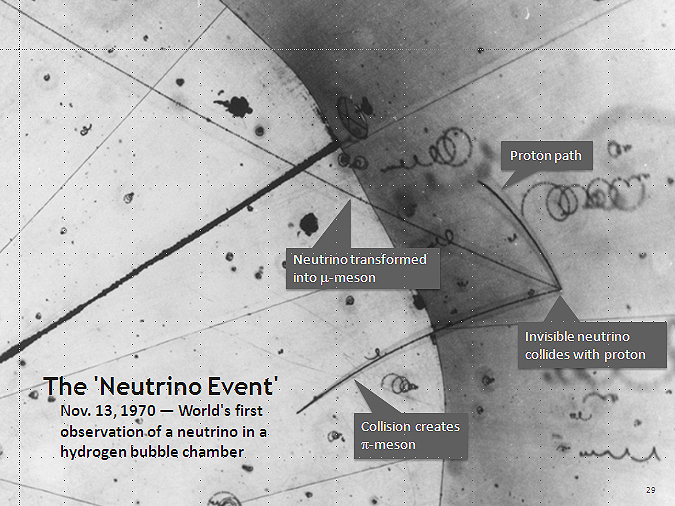
\includegraphics{FirstNeutrinoEventAnnotated.jpg}\hfill}

This project is part of \href{http://neutrino.xyz}{NeuPhysics} . Try \href{http://neutrino.xyz}{http://neutrino.xyz} .

Support us:

{[}DOI: 10.5281/zenodo.27814{]}(\href{https://zenodo.org/badge/latestdoi/7726/NeuPhysics/neutrino}{https://zenodo.org/badge/latestdoi/7726/NeuPhysics/neutrino})

Here is also an index: genindex.html .


\chapter{Preliminary}
\label{preliminary:neutrino-physics}\label{preliminary::doc}\label{preliminary:preliminary}
This chapter is about the preliminary knowledge required by this topic.


\section{Some Interesting Facts}
\label{preliminary:some-interesting-facts}
\begin{notice}{note}{Solar Neutrino Problem}

The sun produces neutrinos inside it and the neutrinos are then propagating out through the plasma. On the earth we can detect them. A problem was that the detected neutrinos were only one third of the total neutrino flux predicted which causes some people to think that the sun had shut down. The solution, however, is the neutrino oscillation.
\end{notice}

As far as we know, we have three flavours of neutrinos and their anti-particles which are  orthogonal to each other,
\begin{gather}
\begin{split}\braket{\nu_{l'}}{\nu_l} &= \delta_{l'l} \\
\braket{\bar\nu_{l'}}{\bar\nu_l} &= \delta_{l'l} \\
\braket{\bar\nu_{l'}}{\nu_l} &= 0.\end{split}\notag
\end{gather}
The interesting thing about neutrinos is that it oscillates.


\section{Reactions Related to Neutrinos}
\label{preliminary:reactions-related-to-neutrinos}\begin{enumerate}
\item {} 
Beta decays, \(n\to p + e^- +\bar \nu\) and \(p\to n + e^+ +\nu\)

\item {} 
Electron capture and positron capture, \(e^- + p\to n+\nu\) and \(e^+ + n \to p + \bar \nu\).

\item {} 
Inverse beta decays, \(\nu+ n \to p+e^-\) and \(\bar\nu + p \to n + e^+\).

\item {} 
Inverses of beta decays, \(\bar\nu + e^- + p \to n\) and \(n+e^++\nu \to n\).

\end{enumerate}


\section{What is a Neutrino Particle?}
\label{preliminary:what-is-a-neutrino-particle}
As Wigner said, a physical particle is an irreducible representation of the Poincaré group. A characteristic of Poincaré group is that mass comes in.

A neutrino particle is better recognized as its mass eigenstate.

In QFT, there are 3 different forms of neutrino mass term, left-handed Majorana, right-handed Majorana and Dirac mass terms.


\section{Chirality and Helicity}
\label{preliminary:chirality-and-helicity}
\index{Helicity}

\subsection{Helicity}
\label{preliminary:index-0}\label{preliminary:helicity}
\textbf{Helicity} is the projection of spin onto direction of momentum,
\begin{gather}
\begin{split}h = \vec J\cdot\hat p = \vec L\cdot\hat p + \vec S\cdot \hat p = \vec S\cdot \hat p,\end{split}\notag
\end{gather}
where
\begin{gather}
\begin{split}\hat p = \frac{\vec p}{\left|\vec p\right|}\end{split}\notag
\end{gather}
A state is called \textbf{right-handed} if helicity is positive, i.e., spin has the same direction as momentum.

\index{Chirality}

\subsection{Chirality}
\label{preliminary:chirality}\label{preliminary:index-1}
\textbf{Chirality} is the eigenstate of the Dirac \(\gamma_5\) matrix, which is explicitly, \footnote{
\href{http://www.quantumfieldtheory.info/ChiralityandHelicityindepth.htm}{*Chirality and Helicity In Depth* by Robert D. Klauber}
}
\begin{gather}
\begin{split}\gamma^5 &= \begin{pmatrix} \mathbf 0 & \mathbf I \\ \mathbf I & \mathbf 0 \end{pmatrix} \\
& = \begin{pmatrix} 0 & 0 & 1 & 0 \\ 0 & 0 & 0 1 \\ 1 & 0 & 0 & 0 \\ 0 & 1 & 0 & 0  \end{pmatrix}.\end{split}\notag
\end{gather}

\section{Majorana or Dirac}
\label{preliminary:majorana-or-dirac}

\subsection{Double Beta Decay}
\label{preliminary:double-beta-decay}

\section{States}
\label{preliminary:states}
\index{Wigner Function}

\subsection{Wigner Function}
\label{preliminary:wigner-function}\label{preliminary:index-2}\begin{figure}[htbp]
\centering
\capstart

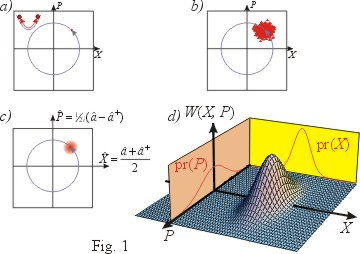
\includegraphics{classicalProbDist.jpg}
\caption{A ensemble of classical harmonic oscillators can be described using such phase-space probability distribution.}\end{figure}

Wigner function is an analogue of the classical phase-space probability distribution function though it is not really probability. \footnote{
\href{http://www.iqst.ca/quantech/wigner.php}{http://www.iqst.ca/quantech/wigner.php}
} The mean of Wigner function lies in the two quadratures, i.e., space distribution and momentum distribution.

There is a collection of Wigner functions on this site. \footnotemark[3]
\begin{description}
\item[{.. admonition:: Question}] \leavevmode\begin{quote}\begin{description}
\item[{class}] \leavevmode
note

\end{description}\end{quote}

How do one describe a system of neutrinos using Wigner function? What is the effect of statistics.

\end{description}


\section{Statistics}
\label{preliminary:statistics}
Fermi-Dirac distribution
\begin{gather}
\begin{split}f(p,\xi) = \frac{1}{1+\exp (p/T-\xi)},\end{split}\notag
\end{gather}
where \(\xi=\mu/T\) is the degeneracy parameter.

The neutrino-neutrino forward scattering is \footnote{
Pantaleone (1992), Friedland \& Lunardini (2003).
}
\begin{gather}
\begin{split}\nu_\alpha (p) + \nu_\beta (k) \to \nu_\alpha (k)+\nu_\beta (p).\end{split}\notag
\end{gather}
\begin{notice}{note}{Question}

Meaning of each term in Liouville equation.
\end{notice}


\section{Questions}
\label{preliminary:questions}
Here are some great questions about neutrinos.

\begin{notice}{note}{Question}

Is neutrino its own antiparticle? Or is neutrino Majorana or Dirac?
\end{notice}

\begin{notice}{note}{Question}

What's the mass hierarchy?
\end{notice}

\begin{notice}{note}{Question}

What are the mixing angles?
\end{notice}

\begin{notice}{note}{Question}

How many different flavours of neutrinos are there?
\end{notice}


\section{Refs \& Notes}
\label{preliminary:refs-notes}

\chapter{Common Sense}
\label{commonsense:common-sense}\label{commonsense::doc}

\section{Units}
\label{commonsense:units}
Natural units makes the calculation of neutrinos convinient. The consequences are
\begin{enumerate}
\item {} 
The energy-mass-momentum relations becomes \(E^2 = p^2 + m^2\). Thus mass \(m\), momentum \(\mathbf p\) and energy \(E\) have the same units.

\item {} 
Angular momentum in quantum mechanics is \(L_z = m\hbar\) where \(m\) is a number. \(\hbar\) is of unit angular momentum.

\item {} 
A plane wave in quantum mechanics is \(\Psi = A e^{ \frac{E t - p x}{\hbar} }\). \(\frac{E t - p x}{\hbar}\) should be unitless, which means \(px\) has unit angular momentum, which is obvious, while \(E t\) also has the unit of angular momentum. Previously we noticed momentum has the same unit with energy, we should have time  \(t\) has the same unit as length \(x\). Also we can conclude that length and time has the unit of \(1/E\).

\end{enumerate}

One should notice that charge is unit 1 in natural units since
\begin{gather}
\begin{split}F = \frac{Qq}{4\pi r^2}.\end{split}\notag
\end{gather}
The conversion between natural units and SI can be down by using the following relations.
\begin{gather}
\begin{split}1 \mathrm{GeV} &= 5.08 \times 10^{15} \mathrm {m^{-1}} \\
1 \mathrm{GeV} &= 1.8\times 10^{-27} \mathrm{kg}\end{split}\notag
\end{gather}

\section{Diagrams}
\label{commonsense:diagrams}\begin{figure}[htbp]
\centering
\capstart

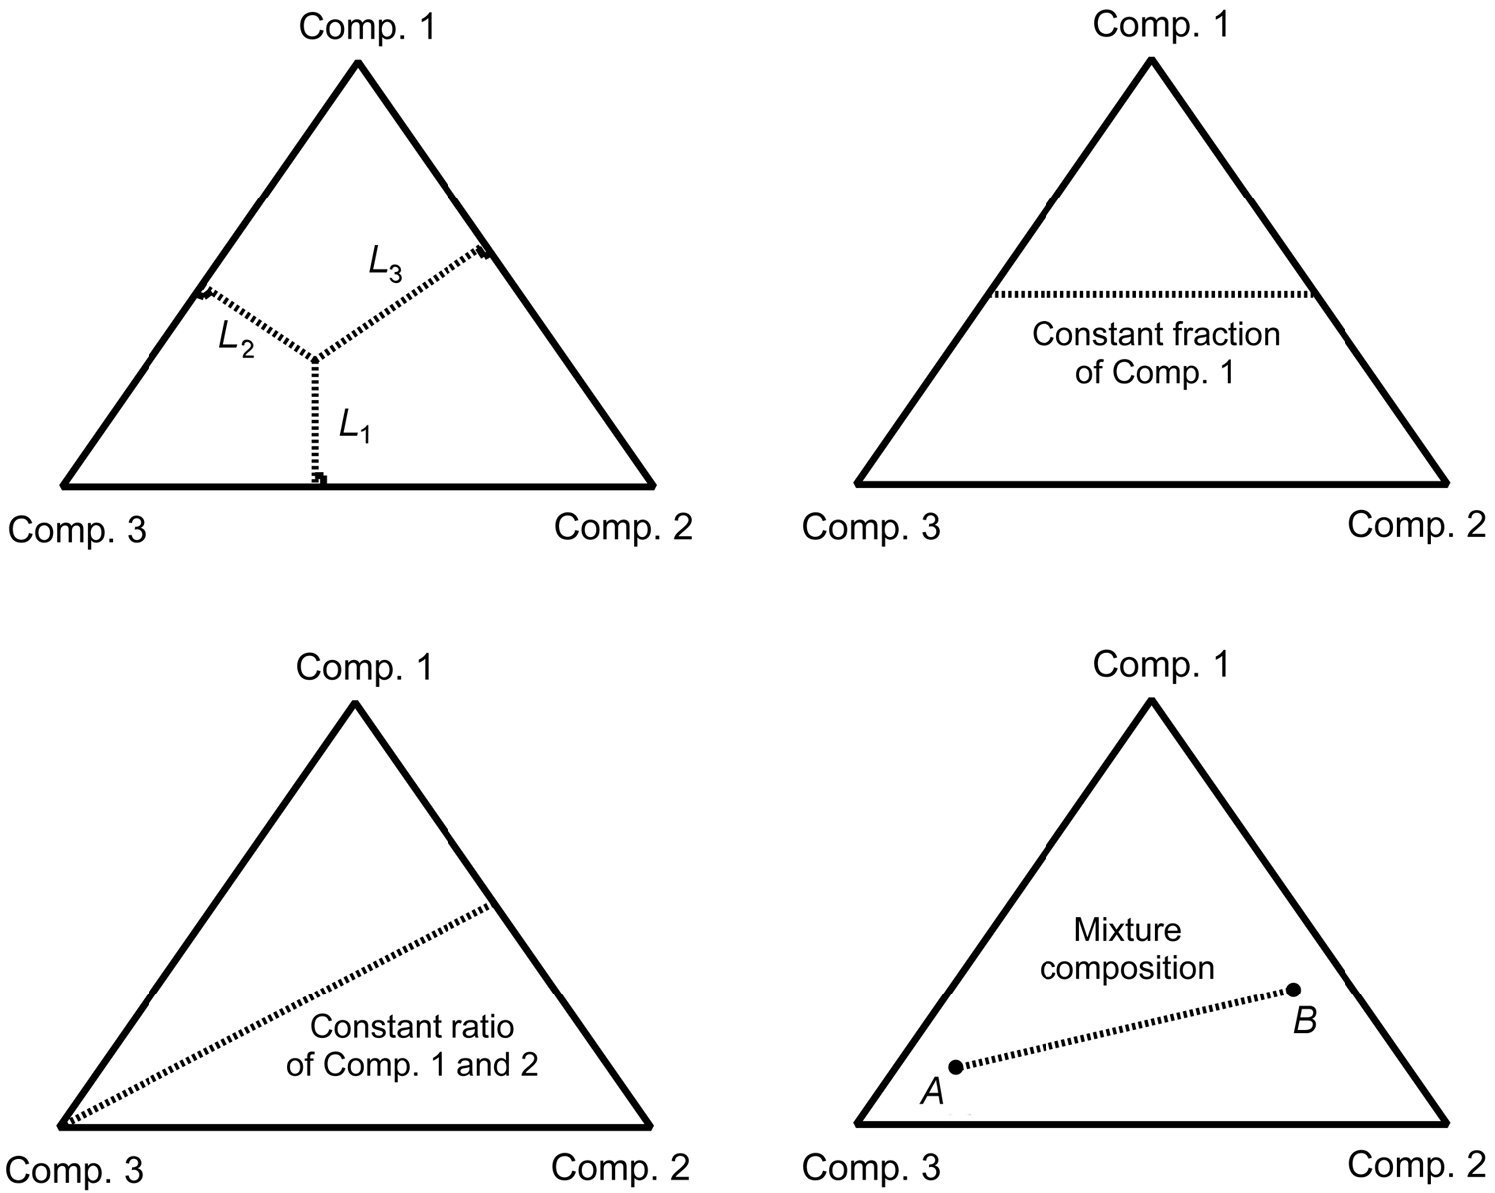
\includegraphics{understandingTernaryDiagram.png}
\caption{The meanings of points and lines in a ternary diagram. From \href{http://petrowiki.org/File\%3AVol1\_Page\_380\_Image\_0001.png}{File:Vol1 Page 380 Image 0001.png@PetroWiki}}\end{figure}

In this documentation on neutrinos, we have all the readings of a point by looking into the line that goes to the left, which means that for the bottom axis, the left is 0 while the right is 1.


\section{Refs and Notes}
\label{commonsense:refs-and-notes}\begin{enumerate}
\item {} 
\href{http://petrowiki.org/Ternary\_phase\_diagrams}{A article about ternary diagram} .

\end{enumerate}


\chapter{Mathematics Related}
\label{math::doc}\label{math:mathematics-related}

\section{The Equations}
\label{math:the-equations}
For 2 flavor oscillations, the equation for flavor neutrinos is
\begin{gather}
\begin{split}i \frac{d}{dt} \begin{pmatrix} \nu_e \\ \nu_x \end{pmatrix} = \frac{\Delta m^2}{4E} \begin{pmatrix} - \cos 2\theta & \sin 2\theta \\  \sin 2\theta  & \cos 2\theta   \end{pmatrix} \begin{pmatrix} \nu_e \\ \nu_x \end{pmatrix}\end{split}\notag
\end{gather}
and with matter
\begin{gather}
\begin{split}i \frac{d}{dt} \begin{pmatrix} \nu_e \\ \nu_x \end{pmatrix} = \frac{\Delta m^2}{4E} \begin{pmatrix} \frac{4E}{\Delta m^2} \sqrt{2} G_F n_e - \cos 2\theta   & \sin 2\theta \\  \sin 2\theta  &  \cos 2\theta   \end{pmatrix} \begin{pmatrix} \nu_e \\ \nu_x \end{pmatrix}\end{split}\notag
\end{gather}
\index{Qualitative Analysis}

\section{Qualitative Analysis}
\label{math:qualitative-analysis}\label{math:index-0}
The vacuum oscillation is determined by autonomous equations. A fixed point of an autonomous system is defined by
\begin{gather}
\begin{split}\frac{d}{dt} \begin{pmatrix} \nu_e \\ \nu_x \end{pmatrix}=0,\end{split}\notag
\end{gather}
which means the so called ``velocity'' is 0. For vacuum oscillation, we set
\begin{gather}
\begin{split}\begin{pmatrix} - \cos 2\theta & \sin 2\theta \\  \sin 2\theta  & \cos 2\theta   \end{pmatrix} \begin{pmatrix} \nu_e \\ \nu_x \end{pmatrix} =0.\end{split}\notag
\end{gather}
Thus we find the fixed points,
\begin{gather}
\begin{split}\nu_e & = 0 \\
\nu_x & = 0.\end{split}\notag
\end{gather}
If we have only the ith function with derivative 0, the line is called the ith-nullcline. Thus the fixed points are the interaction points of all the nullclines.

These fixed points are very useful. In general, for a set of autonomous equations,
\begin{gather}
\begin{split}f'(x) & = F(f,g)\\
g'(x) & = G(f,g),\end{split}\notag
\end{gather}
by definition the fixed point in phase space \(\{f_i,g_i\}\) leads to the result
\begin{gather}
\begin{split}F(f,g) & = 0\\
G(f,g) & = 0.\end{split}\notag
\end{gather}
Thus the equations can be approximated using Taylor expansion near the point \(\{f_i,g_i\}\), since at the fixed points the derivatives are small.
\begin{gather}
\begin{split}\frac{d}{dx} &= F(f,g) \\
& = F(f_i,g_i) + \frac{\partial F(f,g)}{\partial f}\vert_{f=f_i,g=g_i} (f-f_i)+ \frac{\partial F(f,g)}{\partial g}\vert_{f=f_i,g=g_i} (g-g_i)+ \mathcal O(2).\end{split}\notag
\end{gather}
The equations are simplified to linear equations whose coefficient matrix is simply the Jacobian matrix of the original system at the fixed point \(\{f_i,g_i \}\). In this example, the coefficient matrix for the linearized system is
\begin{gather}
\begin{split}\mathbf{C} = \begin{pmatrix} \frac{\partial F(f,g)}{\partial f}\vert_{f=f_i,g=g_i} &   \frac{\partial F(f,g)}{\partial g}\vert_{f=f_i,g=g_i}  \\
\frac{\partial G(f,g)}{\partial f}\vert_{f=f_i,g=g_i}  &  \frac{\partial G(f,g)}{\partial g}\vert_{f=f_i,g=g_i}  \end{pmatrix}.\end{split}\notag
\end{gather}
As a comparison, the Jacobian matrix for the orginal equations at the fixed point is also the same which quite makes sense because Jacobian itself is telling the first order approximation of the velocity.

This linearization is only valid for hyperbolic fixed points which means that the eigenvalues of Jacobian matrix at fixed point has non-zero real part. Suppose the Jacobian is \(\mathbf{J}\) with eigenvalues are \(\lambda_j\), a hyperbolic fixed point requires that \(\mathcal{Re}\lambda_j\neq 0\).

For more analysis, checkout \emph{Poincare-Lyapunov Theorem}.{[}1{]}\_

Define \(p=\mathrm{Tr}(\mathbf{J}(f_i,g_i))\) and \(q=\mathrm{det}(\mathbf{J}(f_i,g_i))\) then the systems can be categorized into 3 different categories given the case that the fixed point isa hyperbolic one.
\begin{figure}[htbp]
\centering
\capstart

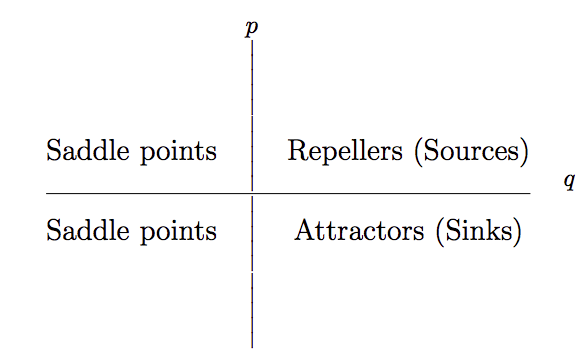
\includegraphics{fixedpoints-massoudmalek.png}
\caption{A diagram that shows the different categorizations given p and q values. Repellers and saddle points are unstable points but attractors are stable. Or in simple ways, given the eigenvalues of the Jacobian \(\lambda_1, \lambda_2\), \(Re(\lambda_1)>0, Re(\lambda_2)>0\) gives us a repeller, \(Re(\lambda_1)<0, Re(\lambda_2)<0\) gives us an attractor while \(Re(\lambda_1)<0, Re(\lambda_2)>0\) gives us the saddle point.}\end{figure}


\chapter{Masses of Neutrinos}
\label{mass::doc}\label{mass:masses-of-neutrinos}
Neutrino masses are still not determined completely. However we have some possible patterns.
\begin{figure}[htbp]
\centering
\capstart

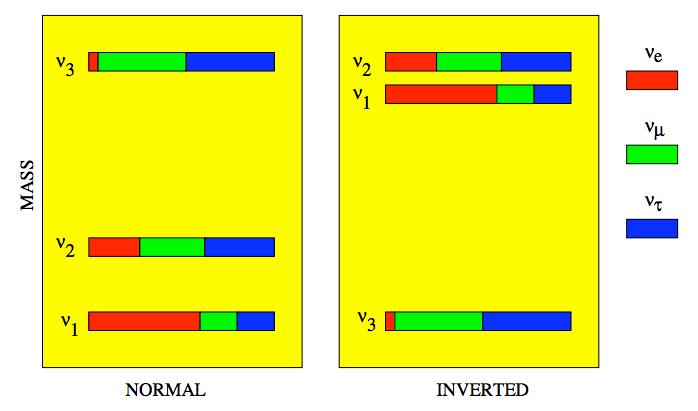
\includegraphics{massPatterns.png}
\caption{Source: \href{http://projects.fnal.gov/nuss/lectures/RabiM\_1.pdf}{http://projects.fnal.gov/nuss/lectures/RabiM\_1.pdf}}\end{figure}

One of the questions we have about the masses of neutrinos is \textbf{the generation of it}.

\begin{notice}{note}{Note:}
This figure also gives the terms: normal hierarchy (NH) and invertd hierarchy (IH).
\end{notice}

Lepton mixing matrix, can be written as the product of three matrices which stands for a rotation in 23, 13(with a CP phase), 12 respectively. This is called the PMNS mixing matrix.
\begin{gather}
\begin{split}\mathbf U &= \mathbf {U_{23}} \times \mathbf {U_{13,\delta}} \times \mathbf {U_{12}} \\
& = \begin{pmatrix} 1 & 0 & 0 \\ 0 &\cos\theta_{23} & \sin\theta_{23} \\ 0 -\sin\theta_{23} & \cos\theta_{23} \end{pmatrix}  \begin{pmatrix} \cos\theta_{13} & 0 & e^{i\delta} \sin\theta_{13} \\ 0 & 1 & 0 \\ -e^{i\delta}\sin\theta_{13} & 0 & \cos\theta_{13}  \end{pmatrix} \begin{pmatrix} \cos\theta_{12} & \sin\theta_{12} & 0 \\ -\sin\theta_{12} & \cos \theta_{12} & 0 \\ 0 & 0 & 1 \end{pmatrix}\end{split}\notag
\end{gather}
\begin{notice}{note}{Neutrino Mixing vs Quark Mixing}

In fact that quarks also has a mixing matrix that mixes the mass eigenstates to produce flavor states. But note that quarks has a mixing matrix of order
\begin{gather}
\begin{split}V_{CKM}\sim \begin{pmatrix}
1 & 0.2 & 0.005 \\
0.2 & 1 & 0.04 \\
0.005 & 0.04 & 1
\end{pmatrix},\end{split}\notag
\end{gather}
while  neutrino has a mixing matrix of order
\begin{gather}
\begin{split}U_{PMNS} \sim \begin{pmatrix}
0.8 & 0.5 & ? \\
0.4 & 0.6 & 0.7 \\
0.4 & 0.6 & 0.7
\end{pmatrix}.\end{split}\notag
\end{gather}
It is obvious that the mixing in neutrino is much larger than quark mixing.
\end{notice}


\section{Experiments}
\label{mass:experiments}
The best fit values in 2014 for the angles in \(\pm 1\sigma\) are
\begin{enumerate}
\item {} 
\(\sin^2\theta_{12}=0.307^{+ 0.018}_{-0.016}\)

\item {} 
\(\sin^2\theta_{23} = 0.386^{+0.024}_{-0.021}\)

\item {} 
\(0.0241\pm 0.0025\).

\end{enumerate}

\index{Majorana Particles}

\section{Majorana Particle}
\label{mass:index-0}\label{mass:majorana-particle}

\subsection{Dirac Equation}
\label{mass:dirac-equation}
Dirac equation can be derived by using the fact that \(E^2=p^2+m^2\) and insisting that the equation should be linear. We start from the assumption
\begin{gather}
\begin{split}i\partial_t \Psi = (\vec\alpha\cdot \vec p + \beta m)\Psi,\end{split}\notag
\end{gather}
where \(\alpha\) and \(\beta\) are NOT necessarily complex numbers. The right side is the energy which comes from the fact that energy operator is \(\hat{E} = i\hbar\frac{\partial}{\partial t} \,\!\).

As we require the energy term satisfy \(E^2=p^2+m^2\), what we have from the assumption is
\begin{gather}
\begin{split}(\vec\alpha\cdot \vec p + \beta m)(\vec\alpha\cdot \vec p + \beta m) \equiv p^2 + m^2.\end{split}\notag
\end{gather}
Expand the expression we get the requirements for \(\vec\alpha\) and \(\beta\),
\begin{gather}
\begin{split}\vec\alpha\cdot\vec \alpha &= 1, \\
\{\alpha_i,\alpha_j\} &= 0, \\
\{\alpha_i,\beta \} & = 0 ,\\
\beta^2 & = 1.\end{split}\notag
\end{gather}
where the second line is for \(i\neq j\).

\begin{notice}{note}{Hint}

Use the component form to derive the requirements.
\end{notice}

\begin{notice}{note}{Quaternion}

A quaternion is a quantity that can be written as a matrix of the form
\begin{gather}
\begin{split}q = \begin{pmatrix}\;z & w \\ -w^* & \;z^*\end{pmatrix}.\end{split}\notag
\end{gather}
As comparison, a complex number can be written as
\begin{gather}
\begin{split}C = \begin{pmatrix}\;\; a &   b  \\- b &  a
\end{pmatrix},\end{split}\notag
\end{gather}
where a and b are real. So quaternion is a generalization of complex number. An important fact is a quaternion times its hermitian conjugate gives us its modulus times an identity, i.e.,
\begin{gather}
\begin{split}q^\dagger q= q q^\dagger = \| q \|^2 I.\end{split}\notag
\end{gather}
Is it useful for Dirac equation?
\end{notice}

These are the most general requirements, any quantities that satisfy the four requirements would do the work.

In fact we have three different representations if we assume \(\vec\alpha\) and \(\beta\) are matrices. They are Dirac-Pauli representation, Weyl representation and Majorana representation.

\begin{notice}{note}{Three representations}

It could be useful to define two four vectors \(\sigma^\mu = (\sigma^0, - \sigma^i)\) and \(\bar\sigma^\mu = (\sigma^0, \sigma^i)\). But all they do is to combine \(\gamma^0\) and \(\gamma^i\) into one expression.
\begin{itemize}
\item {} 
Dirac-Pauli representation

\end{itemize}

The \(\vec\alpha\) and \(\beta\) are
\begin{gather}
\begin{split}\vec \alpha &= \begin{pmatrix} 0 & \vec \sigma \\ \vec\sigma & 0 \end{pmatrix}, \\
\beta & = \begin{pmatrix} I & 0 \\ 0 & -I \end{pmatrix}.\end{split}\notag
\end{gather}
The gamma matrices are
\begin{gather}
\begin{split}\gamma^0 & = \begin{pmatrix} I & 0 \\ 0 & -I  \end{pmatrix}, \\
\gamma^i & = \begin{pmatrix} 0 & \sigma^i \\ -\sigma^i & 0 \end{pmatrix}, \\
\gamma^5 & = \begin{pmatrix} 0 & I \\ I & 0 \end{pmatrix}.\end{split}\notag
\end{gather}
Correspondingly, the chirality operator \(P_{R(+)/L(-)} = \frac{1}{2}(1\pm \gamma^5)\) is
\begin{gather}
\begin{split}P_{L(-)} &=\frac{1}{2} \begin{pmatrix} I & 0 \\ 0 & I  \end{pmatrix},\\
P_{R(+)} & = \frac{1}{2} \begin{pmatrix} I & I  \\ I & I \end{pmatrix}.\end{split}\notag
\end{gather}\begin{itemize}
\item {} 
Weyl representation

\end{itemize}

The \(\vec\alpha\) and \(\beta\) are
\begin{gather}
\begin{split}\vec \alpha &= \begin{pmatrix} -\vec \sigma & 0 \\  0 & \vec\sigma  \end{pmatrix}, \\
\beta & = \begin{pmatrix} 0 & I \\ I & 0 \end{pmatrix}.\end{split}\notag
\end{gather}
The gamma matrices are
\begin{gather}
\begin{split}\gamma^0 & = \begin{pmatrix} 0 & I \\ I & 0  \end{pmatrix}, \\
\gamma^i & = \begin{pmatrix} 0 & \sigma^i \\ -\sigma^i & 0 \end{pmatrix}, \\
\gamma^5 & = \begin{pmatrix} -I & 0 \\ 0 & I \end{pmatrix}.\end{split}\notag
\end{gather}
Correspondingly, the chirality operator \(P_{R(+)/L(-)} = \frac{1}{2}(1\pm \gamma^5)\) is
\begin{gather}
\begin{split}P_{L(-)} &=\frac{1}{2} \begin{pmatrix} I & 0 \\ 0 & 0  \end{pmatrix},\\
P_{R(+)} & = \frac{1}{2} \begin{pmatrix} 0 & 0  \\  0 & I \end{pmatrix}.\end{split}\notag
\end{gather}
In this representation the Dirac equation is
\begin{gather}
\begin{split}(i\partial_t - \vec p \cdot \vec \sigma) \psi_R - m_D\psi_L &= 0, \\
(i\partial_t + \vec p \cdot \vec \sigma) \psi_L - m_D\psi_R &= 0.\end{split}\notag
\end{gather}
where we assumed that
\begin{gather}
\begin{split}\Psi = \begin{pmatrix}  \psi_R \\ \psi_L \end{pmatrix}.\end{split}\notag
\end{gather}
The reason we could have such a simple form of the state is that the chirality operators only take out the upper and lower component of the state. Or in a group theory view, the Poncaré group generators becomes block diagonal and they break up to the generators of \((\frac{1}{2},0)\oplus (0,\frac{1}{2})\). This group theory view also shows that the Dirac representation is reducible and reduces to left and right handed states.
\begin{itemize}
\item {} 
Majorana representation

\end{itemize}

The gamma matrices are
\begin{gather}
\begin{split}\gamma^0 & = \begin{pmatrix} 0 & \sigma^2 \\ \sigma^2 & 0  \end{pmatrix}, \\
\gamma^1 & = \begin{pmatrix} i\sigma^3 & 0 \\ 0 & i \sigma^3  \end{pmatrix}, \\
\gamma^2 & = \begin{pmatrix} 0 & - \sigma^2 \\ \sigma^2 & 0   \end{pmatrix}, \\
\gamma^3 & = \begin{pmatrix} -i\sigma^1 & 0 \\ 0 & -i\sigma^1 \end{pmatrix}, \\
\gamma^5 & = \begin{pmatrix} \sigma^2 & 0 \\ 0 & -\sigma^2 \end{pmatrix}.\end{split}\notag
\end{gather}
The chirality operator \(P_{R(+)/L(-)} = \frac{1}{2}(1\pm \gamma^5)\) won't simplify.

The generators of the Lorentz group becomes all imaginary so that the transformation matrices can be real.
\end{notice}

Dirac equation in D-P rep. is
\begin{gather}
\begin{split}(i\partial_t - \vec p \cdot \vec \sigma) \psi_R - m_D\psi_L &= 0, \\
(i\partial_t + \vec p \cdot \vec \sigma) \psi_L - m_D\psi_R &= 0.\end{split}\notag
\end{gather}
where we use that fact the a state is
\begin{gather}
\begin{split}\Psi = \begin{pmatrix}  \psi_R \\ \psi_L \end{pmatrix}.\end{split}\notag
\end{gather}
\begin{notice}{note}{Charge conjugation}

Charge conjugation can be identified by comparing the equations for a electron and a position. Just plugin the canonical momentum for the four momentum in free Dirac equation. (In Halzen \& Martin section 5.4.) We require that a charge conjugation of a state is
\begin{gather}
\begin{split}\Psi_C = C\gamma^0\Psi^* = C \bar\Psi^T,\end{split}\notag
\end{gather}
where \(C\) is a matrix and \({}^T\) is transposition.

In both D-P and Weyl rep., we have (Halzen \& Martin, excerse 5.6)
\begin{gather}
\begin{split}C = i\gamma^2.\end{split}\notag
\end{gather}
However, in Majorana basis, we have
\begin{gather}
\begin{split}C = I.\end{split}\notag
\end{gather}\end{notice}

\begin{notice}{note}{Parity}

Parity in Weyl basis is
\begin{gather}
\begin{split}\mathscr{P} = \gamma^0.\end{split}\notag
\end{gather}\end{notice}

A Majorana fermion which has the property that its charge conjugation is the same as itself, can be written as
\begin{gather}
\begin{split}\Psi_R &= \begin{pmatrix}  i \sigma^2 \psi_R^* \\ \psi_R  \end{pmatrix}, \\
\Psi_L & = \begin{pmatrix} \psi_L \\  -i\sigma^2\psi_L^* \end{pmatrix}.\end{split}\notag
\end{gather}
\begin{notice}{note}{Why in this form?}

Think about spinor transformation. This form is a spinor. In this case a mass term \(-i\frac{1}{2}( \psi_L^\dagger \sigma^2 \psi_L^* - \psi_L^T \sigma^2 \psi_L )\) becomes \(\frac{m}{2}\bar\Psi_L\Psi_L\).

This will be proved in later context.

Also notice that a charge conjugation in Majorana rep. is identity.
\end{notice}

The equations becomes
\begin{gather}
\begin{split}(i\partial_t -\vec p \cdot \vec \sigma) \psi_R - i m_R \sigma^2 \psi_R^* &= 0, \\
(i\partial_t + \vec p \cdot \vec \sigma) \psi_L - i m_L \sigma^2\psi_L^* & = 0.\end{split}\notag
\end{gather}

\subsection{Lagrangian}
\label{mass:lagrangian}
\begin{notice}{note}{Lagrangian and Equation of Motion}

The Lagrangian with Dirac mass is
\begin{gather}
\begin{split}\mathscr{L}_D = \frac{i}{2} \bar\Psi \overlr{\partial}\Psi - m \bar\Psi \Psi.\end{split}\notag
\end{gather}
Using action principle,
\begin{gather}
\begin{split}\frac{\partial \mathscr{L}}{\partial \bar\Psi} - \partial_\mu \frac{\partial \mathscr{L}}{\partial( \partial_\mu \bar\Psi)} = 0\end{split}\notag
\end{gather}
and the fact that
\begin{gather}
\begin{split}\frac{\partial \mathscr{L}}{\partial\bar\Psi} &= \frac{i}{2} \slashed{\partial} \Psi - m \Psi \\
\frac{\partial \mathscr{L}}{\partial ( \partial_\mu \bar\Psi)} & = -\frac{i}{2} \gamma^\mu \Psi\end{split}\notag
\end{gather}
I have the equation of motion,
\begin{gather}
\begin{split}\frac{i}{2} \slashed{\partial}\Psi - m\Psi + \frac{i}{2}\partial_\mu \gamma^\mu\Psi = 0,\end{split}\notag
\end{gather}
which simplifies to
\begin{gather}
\begin{split}(i\slashed{\partial} - m) \Psi = 0.\end{split}\notag
\end{gather}
Its conjugate is
\begin{gather}
\begin{split}\bar\Psi (\overset\leftarrow{\slashed{\partial}} + m) = 0.\end{split}\notag
\end{gather}
\textbf{In fact we usually drop a surface term in the Lagrangian.} The reason we can do it is because the equation of motion comes from action pricinple. The action is \(S = \int d^4x \mathscr{L}\). Drop or add a surface term to the Lagrangian won't change the equation of motion. The term we would like remove from the Lagrangian is
\begin{gather}
\begin{split}\slashed{\partial} (\bar\Psi \Psi).\end{split}\notag
\end{gather}
The Lagrangian becomes
\begin{gather}
\begin{split}\mathscr{L}_D = \bar\Psi (i\slashed{\partial} ) \Psi -  m \bar\Psi \Psi.\end{split}\notag
\end{gather}\end{notice}

Majorana fermions has more significance when we write down the Lagrangian.

But first, the Lagrangian with Dirac mass term is
\begin{gather}
\begin{split}\mathscr{L}_D = \bar\Psi (i\slashed{\partial} ) \Psi -  m \bar\Psi \Psi,\end{split}\notag
\end{gather}
where \(\bar\Psi = \Psi^\dagger\gamma^0\) and \(\slashed{\partial} = \gamma^\mu \partial_\mu\). Plugin the Weyl representtaion, we have
\begin{gather}
\begin{split}\mathscr{L}_D &= i\begin{pmatrix}\psi_R^\dagger & \psi_L^\dagger \end{pmatrix} \begin{pmatrix} 0 & \sigma^\mu \\  \bar\sigma^\mu & 0 \end{pmatrix} \partial _\mu \begin{pmatrix} \psi_L \\ \psi_R \end{pmatrix} - m\begin{pmatrix}\psi_R^\dagger & \psi_L^\dagger \end{pmatrix}  \begin{pmatrix} \psi_L \\ \psi_R \end{pmatrix} \\
& = i\psi_L^\dagger \bar\sigma^\mu \partial _\mu \psi_L + i \psi_R^\dagger \sigma^\mu \partial_\mu \psi_R - m (\psi_R^\dagger \psi_L + \psi_L^\dagger \psi_R).\end{split}\notag
\end{gather}
where \(\sigma^\mu = (I,-\sigma^i)\) and \(\bar\sigma^\mu = (I,\sigma^i)\). \textbf{Pay attention to the metric when doing contraction.}

This Lagrangian shows the effect of mass which couples the left-handed state and right-handed state.

It is possible to write down another Lagrangian,
\begin{gather}
\begin{split}\mathscr{L}_{M,L} = i\psi_L^\dagger \sigma^\mu \partial_\mu \psi_L + i \frac{1}{2}m( \psi_L^\dagger \sigma^2 \psi_L^* - \psi_L^T \sigma^2 \psi_L),\end{split}\notag
\end{gather}
which decouples the left-handed and right-handed.

\begin{notice}{note}{Global Phase Transformation}

A global phase transformation \(\psi\to e^{i\alpha} \psi\) will change this Lagrangian since we have
\begin{gather}
\begin{split}\psi_L^T\sigma^2 \psi_L \to e^{2i\alpha}\psi_L^T \sigma^2 \psi_L.\end{split}\notag
\end{gather}
Global symmetry is related to charge, in this case Majorana Lagrangian breaks charge conservation law. So Majorana fermions can only be neutral per charge conservation.
\end{notice}

The thing is, this formalism ensures that the charge conjugatioin of a state is itself.


\subsection{Majorana Fermions}
\label{mass:majorana-fermions}
A Majorana fermion is a fermion that obeys the Dirac equation but at the same time doesn't change under charge conjugation, i.e., \(C \Psi^* = \Psi\), where \(C\) is the charge conjugation

\begin{notice}{note}{Charge Conjugation Conventions}

There are at least two different conventions. One is \(\Psi^{(c)} = C \Psi^*\) while the other is \(\Psi^{(c)} = C'\gamma^0 \Psi^*\). In any case, we can prove that in D-P rep., we have
\begin{gather}
\begin{split}C = C'\gamma^0 = i\gamma^2.\end{split}\notag
\end{gather}
In Majorana rep., we have \(C = C'\gamma^0 = I\). From here we can see the importance of Majorana rep..

The way to find this conjugation operator is to use the fact that we requre an electron (with state \(\Psi(p)\)) line in Feynmann diagram is equivalent to a positron (with state \(\Psi^{(c)}(-p)\)) line with opposite momentum so that they have the same charge current. Write down the Dirac equation for both and enforce the to be the same.
\end{notice}

We can work in Weyl basis to find how to write down a genral state. Suppose we have a state that is composed of two Weyl spinors,
\begin{gather}
\begin{split}\Psi = \begin{pmatrix} \psi_1 \\ \psi_2 \end{pmatrix}.\end{split}\notag
\end{gather}
Then we know that in Weyl rep., the charge conjugation is
\begin{gather}
\begin{split}C_{W} = i\gamma^0 = \begin{pmatrix} 0 & i\sigma^2 \\  -i\sigma^2 & 0  \end{pmatrix}.\end{split}\notag
\end{gather}
Apply the representation of \(\Psi\) and \(C_{W}\) in Weyl basis, and use charge conjugation, we have
\begin{gather}
\begin{split}C_W\Psi^* &=  \begin{pmatrix} 0 & i\sigma^2 \\  -i\sigma^2 & 0  \end{pmatrix} \begin{pmatrix} \psi_1^* \\ \psi_2^* \end{pmatrix} \\
& = \begin{pmatrix} i\sigma^2\psi_2^* \\ -i\sigma^2 \psi_1^* \end{pmatrix}.\end{split}\notag
\end{gather}
The condition for Majorana fermions is \(\Psi^{(c)} = \Psi\), which leads to the conclusion that
\begin{gather}
\begin{split}\psi_2 = -i\sigma^2\psi_1^*.\end{split}\notag
\end{gather}
Thus it is possible to have a state that is only composed of one chiral spinor,
\begin{gather}
\begin{split}\Psi = \begin{pmatrix} \psi_L \\ -i\sigma^2 \psi_L^* \end{pmatrix}.\end{split}\notag
\end{gather}
Thus we have decoupled equations for left-handed state and right-handed state.


\subsection{Chirality, Helicity and Spin}
\label{mass:chirality-helicity-and-spin}
For a massless particle, chirality is conserved since the equation of motion or Lagrangian doesn't couple left-handed state with right-handed state.

However, if a particle has mass, chirality symmetry is broken.


\subsection{See-saw Mechanism}
\label{mass:see-saw-mechanism}
In general the mass term in Lagrangian can be written as \footnote{
Elliott, S. R., \& Franz, M. (2015). Colloquium: Majorana fermions in nuclear, particle, and solid-state physics. Reviews of Modern Physics, 87(March), 137–163. doi:10.1103/RevModPhys.87.137
}
\begin{gather}
\begin{split}\mathscr{L}_m = \frac{1}{2} \begin{pmatrix} (\bar\nu_L)^c \bar\nu_R \end{pmatrix}\begin{pmatrix} m_L & m_D \\ m_D & m_R  \end{pmatrix} \begin{pmatrix}  \nu_L \\ (\nu_R)^c \end{pmatrix} + h.c. .\end{split}\notag
\end{gather}
We used the creation and annihilation operators for neutrinos, \(\bar\nu_{L,R}\) and \(\nu_{L,R}\).

\begin{notice}{note}{Annihilation and Creation}

A table in Boris Kayser's paper (arXiv:hep-ph/0211134) shows explicitly the meanings of the operator \footnote{
Kayser, B. (2002). Neutrino Mass, Mixing, and Flavor Change. \href{http://arxiv.org/abs/hep-ph/0211134}{arXiv:hep-ph/0211134} .
}.

\begin{tabulary}{\linewidth}{|L|L|L|}
\hline

Field
 & 
Effect on \(\nu\)
 & 
Effect on \(\bar\nu\)
\\
\hline
\(\nu_{L,R}\)
 & 
Annihilation
 & 
Creation
\\
\hline
\(\bar\nu_{L,R}\)
 & 
Creation
 & 
Annihilation
\\
\hline
\(\nu_{L,R}^{(c)}\)
 & 
Creation
 & 
Annihilation
\\
\hline
\(\bar{\nu_{L,R}}^{(c)}\)
 & 
Annihilation
 & 
Creation
\\
\hline\end{tabulary}

\end{notice}

The idea of see-saw mechanism is to make \(\frac{m_R-m_L}{m_D}\) very large since we do not observe right-handed neutrinos. If we diagonalize the matrix to get to the mass eigenbasis, we have the two eigenvalues of mass should be \(m_R\) and \(\sim m_D^2/m_R\).

The we have the see-saw mechanism. Large mass of right-handed neutrinos compensate the mass of neutrinos we have observe.

The reason that \(\frac{m_R-m_L}{m_D}\) can be large is that \(m_D\) is of the same masses of other leptons because Dirac masses of leptons comes from the same Higgs field.

\begin{notice}{note}{Diagonalizing Mass Matrix}

A mass matrix can be decomposed,
\begin{gather}
\begin{split}\mathscr{M}_\nu = \begin{pmatrix} m_L & m_D \\ m_D & m_R \end{pmatrix} = \begin{pmatrix} 0 & m_D \\ m_D & m_R-m_L \end{pmatrix} + m_L I\end{split}\notag
\end{gather}
I can find the eigenvalues of the masses, they are
\begin{gather}
\begin{split}m_1 & = m_D^2/m_R \\
m_2 & = m_R.\end{split}\notag
\end{gather}
Then we can find the transformation matrix. At this point we can identify that the see-saw mechanism works.

To save time, we can just follow Boris \footnotemark[2] , diagonalizing the first matrix with \((m_R-m_L)/m_D \gg 1\) is done using a unitary matrix
\begin{gather}
\begin{split}Z = \begin{pmatrix} 1 & -\rho \\ \rho & 1  \end{pmatrix} \begin{pmatrix} i & 0 \\ 0 & 1 \end{pmatrix},\end{split}\notag
\end{gather}
where \(\rho=m_D/(m_R-m_L)\) is very small.

The result of the diagonalized mass matrix becomes
\begin{gather}
\begin{split}\mathscr{M}_{\mu,Diag} &= Z^T \mathscr{M}_\nu Z \\
& \approx \begin{pmatrix}  -\frac{m_D^2}{m_R-m_L} & 0 \\  0 & 2\frac{m_D^2}{m_R-m_L}+ m_R-m_L  \end{pmatrix} + m_L I.\end{split}\notag
\end{gather}
\textbf{A problem here.}
\end{notice}


\subsection{Consequences}
\label{mass:consequences}
The see-saw mass term in \eqref{mass-seesaw-mass-lagrangian} combined with the meaning of the creation and annihilation operators, we know that Majorana mass can annihilate a neutrino or antineutrino then create a antineutrino or neutrino.
\begin{figure}[htbp]
\centering
\capstart

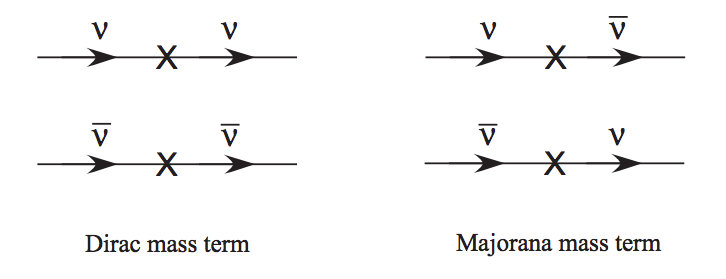
\includegraphics{dirac-mass-vs-majorana-mass-lines.png}
\caption{Figure 1 in \href{http://arxiv.org/abs/hep-ph/0211134}{arXiv:hep-ph/0211134} by Boris Kayser. These diagrams illustrate what Dirac mass and Majorana mass do to the neutrinos.}\end{figure}


\section{Refs \& Notes}
\label{mass:refs-notes}\begin{enumerate}
\item {} 
References for Majorana fermions: \href{http://isites.harvard.edu/fs/docs/icb.topic792163.files/10-spinors.pdf}{Lecture notes by Matthew Schwartz @ Harvard: Lecture 10 Spinors and the Dirac Equation} , \href{http://www.damtp.cam.ac.uk/user/tong/qft/four.pdf}{Lectures notes by Tong @ DAMPTP} .

\end{enumerate}


\chapter{Experiments}
\label{experiments:experiments}\label{experiments::doc}
Chapter 7 (section 7.6) and chapter 12 of Giunti's book \footnote{
Giunti, C., \& Kim, C. W. (2007). Fundamentals of Neutrino Physics and Astrophysics. Oxford University Press. doi:10.1093/acprof:oso/9780198508717.001.0001
} are the good materials to read.

\index{Averaged Transition Probability}

\section{Perdiction of Theory}
\label{experiments:index-0}\label{experiments:perdiction-of-theory}
In experiments we do not directly measure the exact survival probabilty, instead we measure events that are generated by neutrinos. The connection between the theoretical exact survival probability is to average over the parameters that we do not precisely resolve.

In the example of 2 flavor oscillation, the transition probability from \(\nu_\alpha\) to \(\nu_\beta\) is given by
\begin{gather}
\begin{split}P_{\alpha\to\beta}(L,E) = \frac{1}{2}\sin^2 2\theta_v\left( 1 - \cos\left( \frac{\Delta m^2}{2}\frac{L}{E} \right) \right).\end{split}\notag
\end{gather}
It is not possible to obtain this result since we do not have enough resolution for \(L\) and \(E\). The observed result is the probability averaged over the distribution of \(L\) and \(E\). \footnotemark[1]

Nonetheless, in this simple two flavor example, the probability only depends on \(\frac{L}{E}\). So we average over \(\frac{L}{E}\). \footnotemark[1]
\begin{gather}
\begin{split}\langle P_{\alpha\to\beta}(L/E) \rangle = \int P_{\alpha\to\beta}(L/E) \phi(L/E) d(L/E),\end{split}\notag
\end{gather}
where \(\phi(L/E)\) is the distribution.

The practical distribution of \(\frac{L}{E}\) is Gaussian, \footnotemark[1]
\begin{gather}
\begin{split}\phi(\frac{L}{E}) = \frac{1}{\sqrt{2\pi \sigma_{L/E}^2}} \exp\left( -\frac{(L/E - \langle L/E\rangle)^2}{2\sigma_{L/E}^2} \right),\end{split}\notag
\end{gather}
which determines the average of the cosine term is \footnotemark[1]
\begin{gather}
\begin{split}\langle \cos \left(\frac{\Delta m^2}{2} \frac{L}{E} \right)\rangle = \cos\left( \frac{\Delta m^2}{2} \langle \frac{L}{E} \rangle \right)\exp\left( -\frac{1}{2}\left( \frac{\Delta m^2}{2} \sigma_{L/E} \right)^2 \right).\end{split}\notag
\end{gather}
\begin{notice}{note}{Variance of L/E}

The virance can be splitted into two parts,
\begin{gather}
\begin{split}\left( \frac{\sigma_{L/E}}{\langle L/E\rangle} \right)^2 = \left( \frac{\sigma_L}{\langle L\rangle} \right)^2 + \left( \frac{\sigma_E}{\langle E\rangle} \right)^2,\end{split}\notag
\end{gather}
which comes from the fact that a Gaussion is written as
\begin{gather}
\begin{split}\propto \exp\left( \frac{1}{2} \left( \frac{b}{\sigma_b} - \frac{\langle b\rangle}{\sigma_b} \right)^2 \right).\end{split}\notag
\end{gather}\end{notice}


\subsection{What Does A Detector Do}
\label{experiments:what-does-a-detector-do}
In experiments we can either detect the appearance of \(\nu_\alpha\) or find the disappearance of \(\nu_\alpha\) given a source of \(\nu_\beta\).

If a detector can not observe any oscillations, that means it can only put a upper limit on the averaged probability. \textbf{Otherwise the detector will find exactly the averaged probability!}

That being said, the averaged probability obtains an upper limit through experiments,
\begin{gather}
\begin{split}\langle P_{\alpha\to\beta}(L,E) \rangle \leq P_{\alpha\to\beta}^{max},\end{split}\notag
\end{gather}
which in 2 flavor case is
\begin{gather}
\begin{split}\sin^2 2\theta_v \left( 1- \langle \cos\left( \frac{\Delta m^2}{2} \frac{L}{E} \right) \rangle \right)   \leq P_{\alpha\to\beta}^{max}\end{split}\notag
\end{gather}
Using Gaussian distribution of \(\phi(L/E)\), we have \footnotemark[1]
\begin{gather}
\begin{split}P_{\alpha\to\beta} = \frac{1}{2} \sin^2 2\theta_v \left( 1 - \cos \left( \frac{\Delta m^2}{2} \langle \frac{L}{E}\rangle \right) \exp\left( -\frac{1}{2} \left( \frac{\Delta m^2}{2} \sigma_{L/E} \right)^2 \right) \right) \leq P_{\alpha\to\beta}^{max}.\end{split}\notag
\end{gather}
The relation between \(\sin^2 2\theta_v\) and \(L/E\) can be found,
\begin{gather}
\begin{split}\sin^2 2\theta_v \leq \frac{2 P_{\alpha\to\beta}^{max} }{1 - \cos \left( \frac{\Delta m^2}{2} \langle \frac{L}{E}\rangle \right) \exp\left( -\frac{1}{2} \left( \frac{\Delta m^2}{2} \sigma_{L/E} \right)^2 \right) },\end{split}\notag
\end{gather}
in a simple equation,
\begin{gather}
\begin{split}\sin^2 2\theta_v \leq f(\Delta m^2 \langle \frac{L}{E} \rangle ).\end{split}\notag
\end{gather}
This relation allows us to do a joint analysis of \(\sin^2 2\theta_v\) and \(\Delta m^2\).

\begin{notice}{note}{General Form of Constraint}

Rewrite
\begin{gather}
\begin{split}\sin^2 2\theta_v \left( 1- \langle \cos\left( \frac{\Delta m^2}{2} \frac{L}{E} \right) \rangle \right)   \leq 2 P_{\alpha\to\beta}^{max},\end{split}\notag
\end{gather}
we have
\begin{gather}
\begin{split}\sin^2 2\theta_v    \leq  \frac{ 2 P_{\alpha\to\beta}^{max} }{ \left( 1- \langle \cos\left( \frac{\Delta m^2}{2} \frac{L}{E} \right) \rangle \right) }\end{split}\notag
\end{gather}\end{notice}

\index{Exclusion Curve}\begin{figure}[htbp]
\centering
\capstart

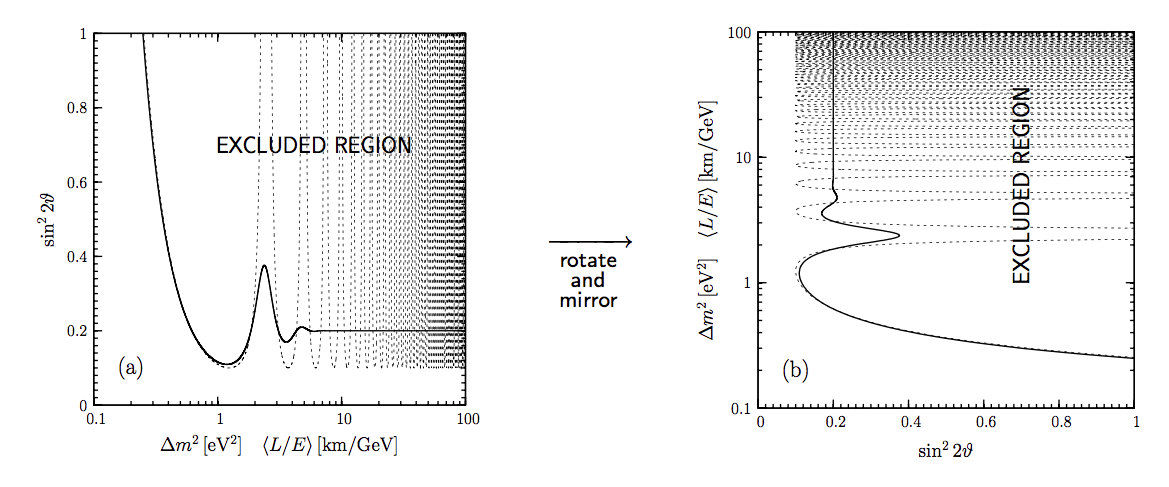
\includegraphics{sinSquare2thetaVSDeltamSquare.png}
\caption{A figure grabbed from Giunti's book \emph{Fundamentals of Neutrino Physics and Astrophysics} section 7.6. As we mentioned, we have a relation between \(\sin^2 2\theta_v\) and \(\Delta m^2\), which is given as the black solid lines in the figures. The regions that have larger values of \(\sin ^2 2\theta_v\) are excluded. Thus the solid lines are called exclusion curve.}\label{experiments:index-1}\end{figure}


\subsection{The Stringent Constraint of Mixing Angle}
\label{experiments:the-stringent-constraint-of-mixing-angle}
The most stringent constraint for \(\sin^2 2\theta_v\) happens when the demoninator of the right side is largest, which means
\begin{gather}
\begin{split}\langle \cos \left( \frac{\Delta m^2}{2} \frac{L}{E}  \right) \rangle = -1.\end{split}\notag
\end{gather}
\begin{notice}{note}{Averge of cosine}

In experiments, we have the fact that the change in \(\frac{L}{E}\) is small compared to the average value \(\langle\frac{L}{E}\rangle\).

So when we average over the cosine
\begin{gather}
\begin{split}\langle \cos \left( \frac{\Delta m^2}{2} \frac{L}{E}  \right) \rangle,\end{split}\notag
\end{gather}
we actually can assume that we are averaging over the argument. The reason is that we can do Taylor expansion and drop all terms except the zeroth order since the change in argument is small.

In the language of math,
\begin{gather}
\begin{split}\left\langle  \left( \frac{L}{E} - \left\langle \frac{L}{E} \right\rangle  \right)^2 \right\rangle \ll \left( \left\langle \frac{L}{E} \right\rangle  \right)^2.\end{split}\notag
\end{gather}
The left hand side can be expanded to
\begin{gather}
\begin{split}\langle \left(\frac{L}{E} \right)^2 \rangle - \langle \frac{L}{E}\rangle^2,\end{split}\notag
\end{gather}
which is pluged into the inequality. We have finally
\begin{gather}
\begin{split}\langle \left(\frac{L}{E} \right)^2 \rangle \ll 2\langle \frac{L}{E}\rangle^2.\end{split}\notag
\end{gather}\end{notice}

The condition leads to
\begin{gather}
\begin{split}\cos\left( \frac{\Delta m^2}{2} \langle \frac{L}{E} \rangle \right) = -1.\end{split}\notag
\end{gather}
Solving this equation we know the condition for the most stringent constraint on \(\sin^2 2\theta_v\) happens when
\begin{gather}
\begin{split}\frac{\Delta m^2}{2} \langle \frac{L}{E} \rangle \sim \pi,\end{split}\notag
\end{gather}
which is
\begin{gather}
\begin{split}\Delta m^2 \langle \frac{L}{E} \rangle \sim 2\pi.\end{split}\notag
\end{gather}
\begin{notice}{note}{Units of \(\Delta m^2  L/E\)}

First of all, calculate the following expression,
\begin{gather}
\begin{split}&1 eV^2 \frac{1km}{1GeV} \\
=& 1eV^2 \frac{10^{18}fm}{10^8 eV} \\
=& 1eV^2 \frac{10^{18}}{10^8 eV} \frac{1}{197 MeV} \\
=& \frac{1}{1.97}.\end{split}\notag
\end{gather}
Thus we have
\begin{gather}
\begin{split}\Delta m^2   \frac{L}{E} = \frac{1}{1.97} \left( \frac{\Delta m^2}{1eV^2} \right) \left(  \frac{L/1km}{E/1GeV} \right).\end{split}\notag
\end{gather}\end{notice}

Rewrite it using the Bethe trandition,
\begin{gather}
\begin{split}\left( \frac{\Delta m^2}{1eV^2} \right) \left(  \frac{L/1km}{E/1GeV} \right) \sim \frac{2\pi}{1.97} = 1.24.\end{split}\notag
\end{gather}

\subsection{Small \(\Delta m^2 \langle L/E \rangle\) Limit}
\label{experiments:small-limit}
In small \(\Delta m^2 \langle L/E \rangle\) limit, we have the Taylor expansion of cosine term
\begin{gather}
\begin{split}\langle \cos \left( \frac{\Delta m^2}{2} \frac{L}{E} \right)\rangle \approx \langle 1- \frac{1}{2}\left( \frac{\Delta m^2}{2} \frac{L}{E} \right)^2 \rangle  \approx 1 - \frac{1}{2} \left(\frac{\Delta m^2}{2} \right)^2 \langle \left( \frac{L}{E} \right)^2 \rangle.\end{split}\notag
\end{gather}
Using the Gaussian distribution result, we reach a constraint
\begin{gather}
\begin{split}\sin^2 2\theta_v \leq \frac{2 P_{\alpha\to\beta}^{max} }{\frac{1}{2} \left( \frac{\Delta m^2}{2}  \right)^2 \langle \left(\frac{L}{E}\right)^2 \rangle}.\end{split}\notag
\end{gather}
As we have discussed before,
\begin{gather}
\begin{split}\langle \left(\frac{L}{E} \right)^2 \rangle \ll 2\langle \frac{L}{E}\rangle^2,\end{split}\notag
\end{gather}
which leads to
\begin{gather}
\begin{split}\sin^2 2\theta_v \leq \frac{2 P_{\alpha\to\beta}^{max} }{ \left( \frac{\Delta m^2}{2}  \right)^2  \left(\langle\frac{L}{E} \rangle\right)^2 },\end{split}\notag
\end{gather}
\begin{notice}{note}{Giunti's Results}

Giuti's idea is that
\begin{gather}
\begin{split}\langle \left(\frac{L}{E} \right)^2 \rangle - \langle \frac{L}{E}\rangle^2 \ll 2\langle \frac{L}{E}\rangle^2\end{split}\notag
\end{gather}
basically means
\begin{gather}
\begin{split}\langle \left(\frac{L}{E} \right)^2 \rangle - \langle \frac{L}{E}\rangle^2 \sim 0,\end{split}\notag
\end{gather}
which leads to the result that
\begin{gather}
\begin{split}\langle \left(\frac{L}{E} \right)^2 \rangle \sim \langle \frac{L}{E}\rangle^2.\end{split}\notag
\end{gather}
Then he has
\begin{gather}
\begin{split}\sin^2 2\theta_v \leq \frac{2 P_{\alpha\to\beta}^{max} }{ \frac{1}{2} \left( \frac{\Delta m^2}{2} \right)^2  \left(\langle\frac{L}{E} \rangle\right)^2 }.\end{split}\notag
\end{gather}\end{notice}


\subsection{Large \(\Delta m^2 \langle L/E \rangle\) Limit}
\label{experiments:large-limit}
In this limit, we have a flat line in the \(\sin^2 2\theta_v\) vs \(\Delta m^2 \langle\frac{L}{E}\rangle\) plot.

The reason is that the limit of \(\sin^2 2\theta_v\) becomes
\begin{gather}
\begin{split}\sin^2 2\theta_v \leq 2  P_{\alpha\to\beta}^{max}.\end{split}\notag
\end{gather}
\begin{notice}{note}{Reason for Flat Line}

The exponential part dominates and the denominator becomes 1 at large \(\Delta m^2 \langle L/E \rangle\) value.
\end{notice}


\section{Sensitivity}
\label{experiments:sensitivity}
\begin{notice}{note}{Sensitivity}

\((\sin^2 2\theta_v)_s\) and \((\Delta m^2)_s\) are better at small values because they means the ``smallest'' constraint we can obtain.
\begin{figure}[htbp]
\centering
\capstart

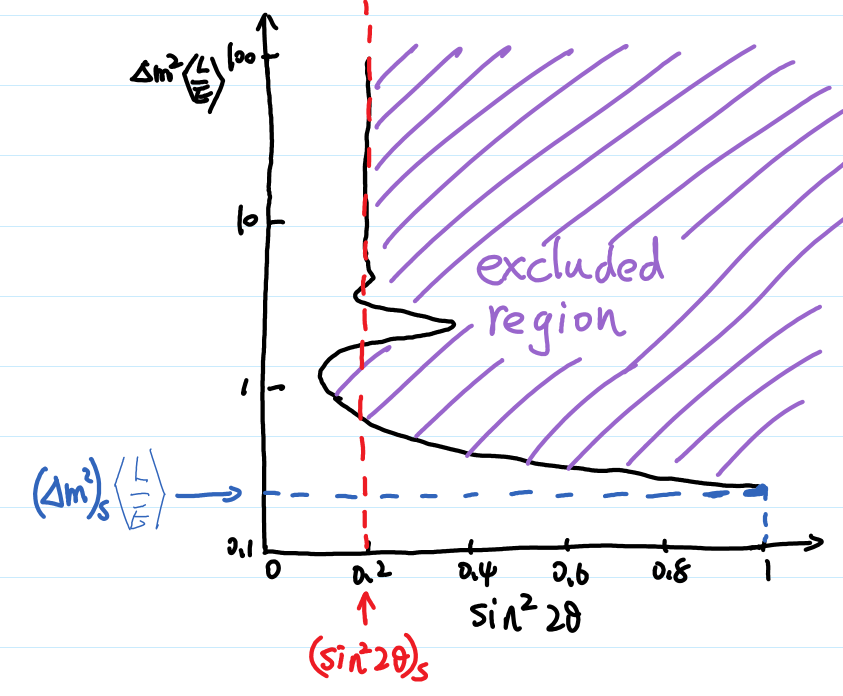
\includegraphics{exclusionCurveSensitivity.png}
\caption{Sensitivities}\end{figure}
\end{notice}

For disappearance experiments:
\begin{itemize}
\item {} 
L \(\searrow\) : \((\sin^2 2\theta_v)_s\) \(\searrow\), \((\Delta m^2)_s\) \(\nearrow\); (going up means sensitivity becomes worse; going down means sensitivity becomes better.)

\item {} 
E \(\searrow\) : \((\sin^2 2\theta_v)_s\) \(\searrow\), \((\Delta m^2)_s\) \(\searrow\).

\end{itemize}

We have very little control over the production energy of neutrinos though. To have a better sensitivity of mass difference (i.e., make the sensitivity values smaller), we need to have a bigger distance, which makes the sensitivity of mixing angles worse. But we can at the same time increase the flux of \(\nu_\alpha\) and the mass of the detector to compensate this loss of sensitivity.


\section{Review of Experiments}
\label{experiments:review-of-experiments}
Through the analysis we know that the most important factors of experiments are
\begin{itemize}
\item {} 
Basiline \(L\);

\item {} 
Source neutrino flux;

\item {} 
Neutrino energy \(E\).

\end{itemize}


\subsection{Reactor Experiments}
\label{experiments:reactor-experiments}
What we would like to see in the experiments is the disappearance of the reactor neutrinos. In nuclear fusion we have a lot of \(\bar\nu_e\) which will oscillate to other flavors. If the detector is sensitive enough we would find out that the detected neutrinos are smaller than the expected neutrinos without oscillation.

The energy of the neutrinos is about 1.8MeV.

The first question is how many neutrinos can be detected. If neutrino energy is too high, cross section at detector will be large but neutrino flux per unit energy will be small. The best detection rate is at some certain energy.
\begin{figure}[htbp]
\centering
\capstart

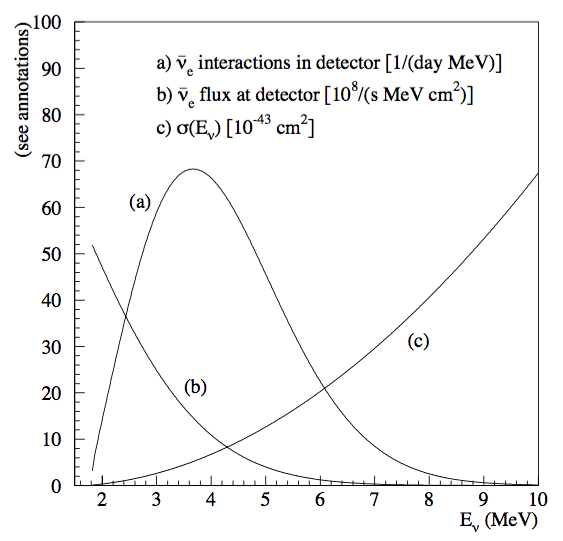
\includegraphics{reactorDetection.png}
\caption{The best energy of detection. Figure 12.2 in Giunti's book.}\end{figure}

\begin{notice}{note}{The Source Flux}

We can calculate the production of neutrinos by monitoring the power of the nuclear reactor.
\end{notice}
\begin{figure}[htbp]
\centering
\capstart

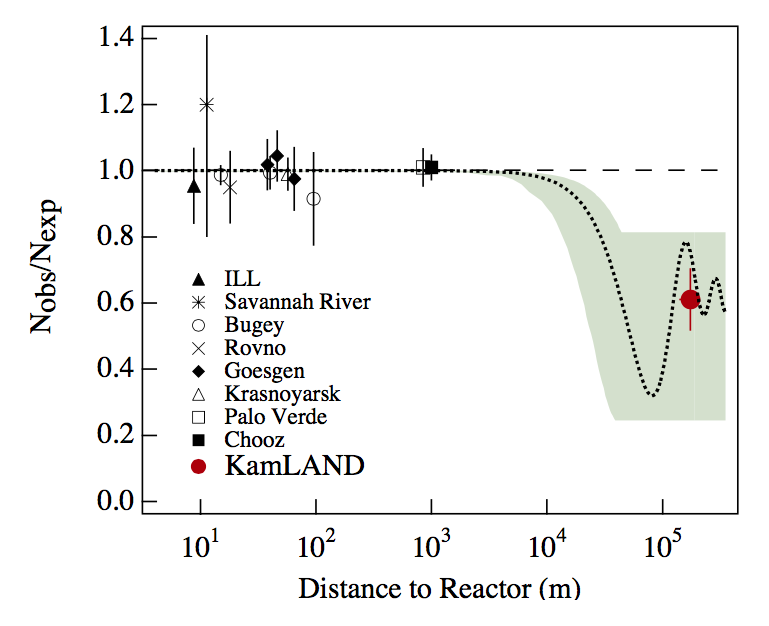
\includegraphics{reactorExpBaseline.png}
\caption{The ratio of observed neutrino flux to expected neutrino flux compared in different experiments. The dotted line is the ratio when expected flux calculated from best fit results of \(\Delta m^2\) and \(\sin^2 2\theta_v\) extracted from solar neutrino experiments. These experiments more or less lie on the best fit result. Figure 12.3 of Giunti's book.}\end{figure}
\begin{itemize}
\item {} 
\(L\sim 10 - 100 m\) : short baseline experiment (SBL);

\item {} 
CHOOZ and Palo Verde has baseline \(L\sim 1km\) : long baseline experiment (LBL);

\item {} 
KamLAND has baseline \(L\sim 200km\) : Very long baseline experiment (VLBL).

\end{itemize}

To find the best result of mass squared difference \(\Delta m^2\), we need a long baseline like KamLAND.

\begin{notice}{note}{Background}

One of the background of neutrinos is the cosmic ray. The cosmic neutrino background is much smaller than the reactor neutrino flux.
\begin{figure}[htbp]
\centering
\capstart

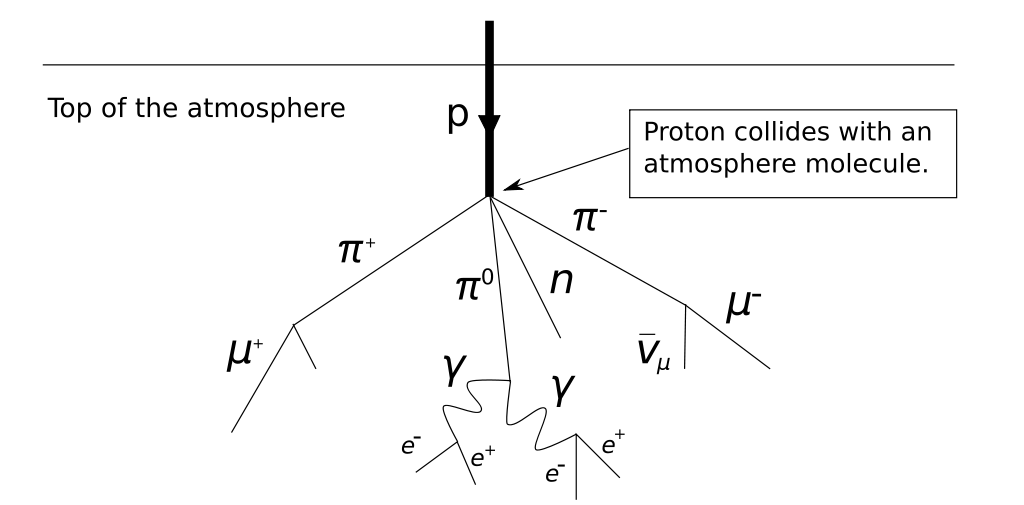
\includegraphics{atmosphericNeutrinos.png}
\caption{Production of neutrinos through cosmic rays. We need to shield the hardons. From \href{https://commons.wikimedia.org/wiki/File:Atmospheric\_Collision.svg}{wikipedia}.}\end{figure}

The background actually can be measured when the nuclear plants are turned off to supply fuel.
\end{notice}


\subsubsection{Review of Reactor Experiments}
\label{experiments:review-of-reactor-experiments}
Experiments can detect antielectron neutrinos through inverse neutron decay (inverse beta decay),
\begin{gather}
\begin{split}\bar\nu_e + p \to n + e^+ .\end{split}\notag
\end{gather}\begin{itemize}
\item {} 
Late 1970s to the 1990s, SBL experiments with detector mass of order \(10^2\mathrm{kg}\) got null results, i.e., they didn't find the disappearance of the reactor neutrinos which is \(\bar\nu_e\). The reason is that they have short baseline. The result is \(\Delta m^2\sim 10^{-2}\mathrm{eV^2}\).

\item {} 
LBL experiments gave us better exclusion curves.
* \textbf{CHOOZ} : 5 tons of detector mass; 1115km and 998m from the two sources.
* \textbf{Palo Verde} : 12 tons of detector mass; 890m, 890m and 750m from the three sources.

\item {} 
\textbf{KamLAND}: mostly detects neutrinos from 53 reactors in Japan. 80\% neutrinos from reactors at distance between 140km and 215km.  3000 tons of detector mass. Best fit results using KamLAND and solar neutrino is \(\Delta m^2 = 7.9^{+0.6}_{0.5}\times 10^{-5}\mathrm{eV^2}\) and \(\tan^2\theta_v = 0.40^{+0.10}_{-0.07}\), which corresponds to \(\sin^2 2\theta_v \sim 0.82\).

\end{itemize}
\begin{figure}[htbp]
\centering
\capstart

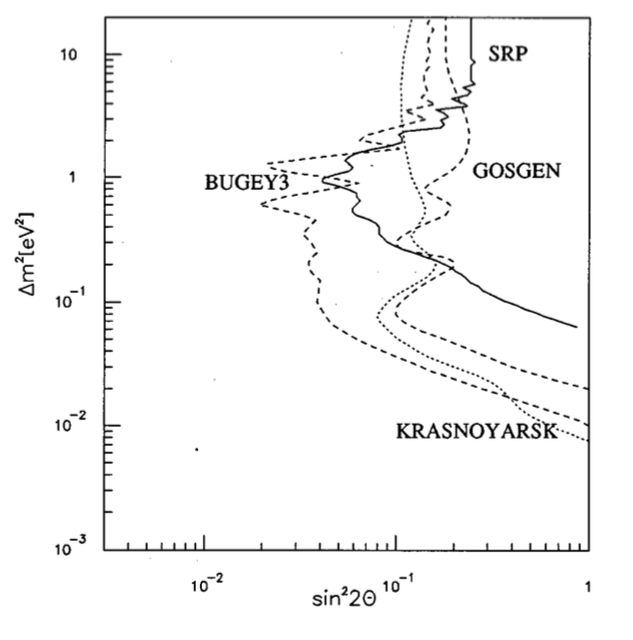
\includegraphics{sblResults.png}
\caption{SBL results from Giunti's book (figure 12.5). These experiments showed exclusion curves that extend to \(\Delta m^2\sim 10^{-2}\mathrm{eV^2}\).}\end{figure}
\begin{figure}[htbp]
\centering
\capstart

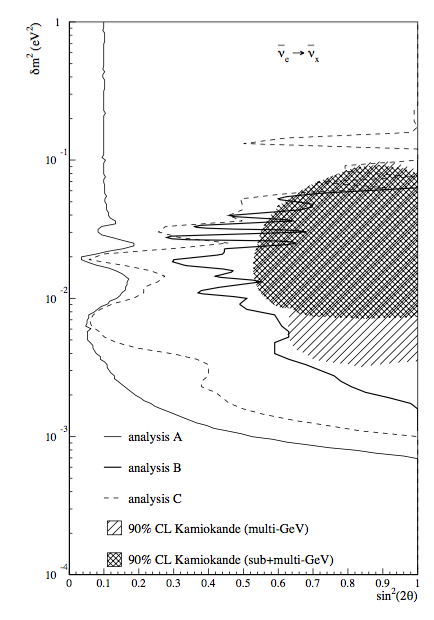
\includegraphics{choozResult.png}
\caption{CHOOZ result from Giunt's book (figure 12.6).}\end{figure}
\begin{figure}[htbp]
\centering
\capstart

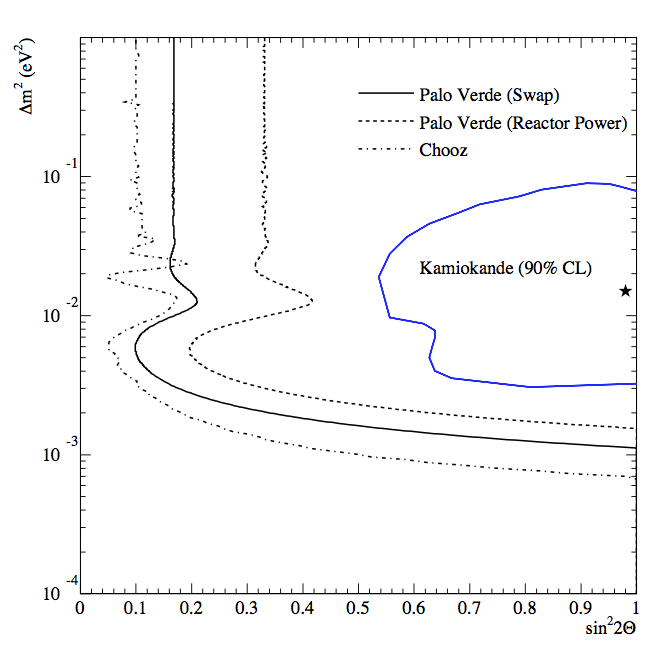
\includegraphics{paloVerdeResult.png}
\caption{Palo Verde result from Giunt's book (figure 12.7).}\end{figure}
\begin{figure}[htbp]
\centering
\capstart

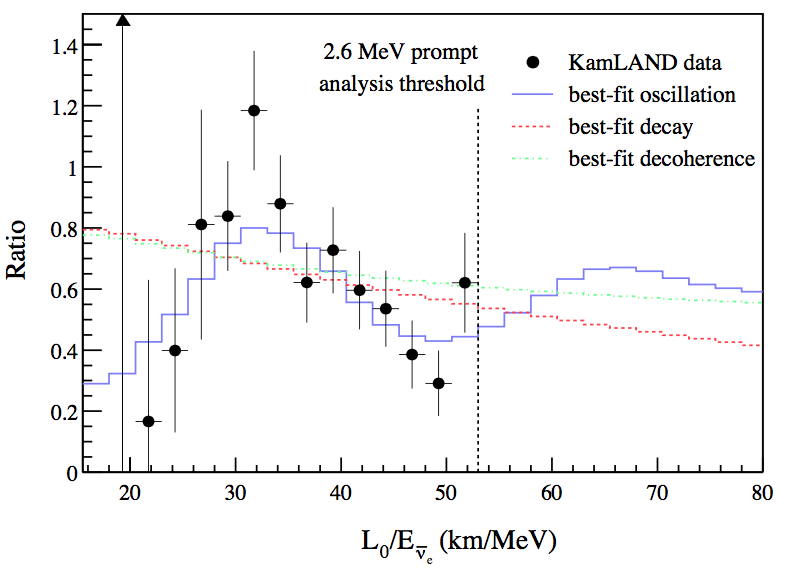
\includegraphics{kamLANDOsc.png}
\caption{KamLAND detected the oscillation. To calculate the expected flux, the experiment used \(L_0 = 180 \mathrm {km}\). The best fit is \(\Delta m^2 7.9^{+0.6}_{-0.5} times 10^{-5}\mathrm{eV^2}\).  From Giunti figure 12.9.}\end{figure}
\begin{figure}[htbp]
\centering
\capstart

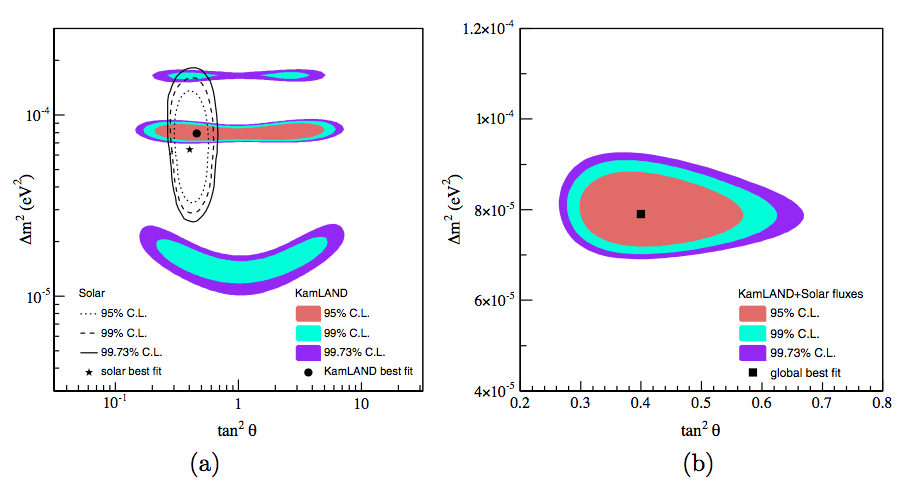
\includegraphics{kamLANDResults.png}
\caption{KamLAND result from  Giunt's book (figure 12.10). The left figure is the result of KamLAND while the result is the joint analysis of KamLAND and solar neutrino using 2 neutrino oscillation.}\end{figure}


\subsection{Accelerator Experiments}
\label{experiments:accelerator-experiments}\begin{itemize}
\item {} 
WB : wide band = wide energy spectrum;

\item {} 
NB : narrow band = narrow energy spectrum;

\item {} 
OA : off-axis to obtain almost monochromatic beam.

\end{itemize}


\section{Low Energy Neutrino Detection}
\label{experiments:low-energy-neutrino-detection}\begin{enumerate}
\item {} 
{[}KATRIN{]}(\href{https://www.katrin.kit.edu/}{https://www.katrin.kit.edu/})

\item {} 
Project 8

\item {} 
PROLEMY

\end{enumerate}


\section{Refs \& Notes}
\label{experiments:refs-notes}

\chapter{How Do Neutrinos Propagate}
\label{propagation::doc}\label{propagation:how-do-neutrinos-propagate}
\begin{notice}{note}{Question}

How to interpret neutrino propagation and scattering using wave packet formalism?
\end{notice}

In the book of \emph{Principles of Quantum Mechanics}, Shankar shows how to deal with scattering using just wave packet.

What I can do is to check the following questions.
\begin{enumerate}
\item {} 
How do wave packet formalism help us understanding the scattering of neutrinos.

\item {} 
How do relativistic case change the results?

\item {} 
What if the packet is a combination of Gaussian packets?

\end{enumerate}

\index{Wave Packet Treatment}

\section{Wave Packet Treatment}
\label{propagation:wave-packet-treatment}\label{propagation:index-0}
From uncertainty principle we know it's not good enough to treat neutrinos as mono-momentum particles because our measurement measures the momentum with an accuracy and the position of the neutrinos are not completely determined. We have both momentum width and position width which looks a lot like a wave packet.

The caveats are
\begin{enumerate}
\item {} 
What are the energies, momenta, velocities of neutrinos and the average of them?

\item {} 
How to find the amplitude of wave packet? What's the geometry of the wave packet?

\item {} 
The time evolution should reduce to the single particle formalism in some limits.

\end{enumerate}

In principle we need all the information about the generation of neutrinos. However, we can use some unknown paramters to derive the formalism of the wave packets then investigate the unknown paramters.

A wave packet is constructed with a distribution of amplitude at each momentum and position and time.

\begin{notice}{note}{Note:}
A wave packet in wave dynamics is bunch of plane waves that makes a localized packet. For example one of the general form of wave packets is
\begin{gather}
\begin{split}u(x,t) = \frac{1}{\sqrt{2\pi}} \int^{\,\infty}_{-\infty} A(k) ~ e^{i(kx-\omega(k)t)} \,dk .\end{split}\notag
\end{gather}
Basically, one needs a lot of frequencies/wavenumbers/momenta to construct some localized waves.
\end{notice}

As an application of this general wave packet, we can write down the wave packet of neutrinos using an assumed initial distribution over all possible momenta. \textbf{The problem is that we have no idea what the amplitude should be.}


\subsection{Some Questions}
\label{propagation:some-questions}
Some questions should be answered in this formalism.
\begin{enumerate}
\item {} 
What are \(\nu_f\) and \(\nu_m\) in this formalism?

\end{enumerate}

\begin{notice}{note}{Question}

What is \(\nu_f\), i.e., the flavour state, in the formalism of wave packet?
\end{notice}

\begin{notice}{note}{Answer}

In the view of math, the flavour state is a superposition of all mass states,
\begin{gather}
\begin{split}\psi(x,t) = \int_{lower}^{upper} dp_\nu' \sum_m U_{fm} a(p_\pi^m(p_\nu')) \nu_m e^{ip_\nu'x} e^{-i E_m(p_\nu')t}\end{split}\notag
\end{gather}
In other words, as long as we can measure the wave packet in a sense that the position difference is large enough, the wave packet still.
\end{notice}

\begin{notice}{note}{Question}

What does decoherence mean then?
\end{notice}

\begin{notice}{note}{Answer}

An first idea can be that the wave packets of different mass eigen states are travelling at different speed thus they get very far apart after some travelling time.

However we should be careful with the wave packet formalism. This treatment is infact an effective treatment in my understanding, to reconcile the fact that the neutrinos are actually not at a definite position and momentum state due to quantum uncertainty principle.

So any discussion about the decoherence of the wave packets should make clear of the measurements including the production procedure.
\end{notice}

.


\chapter{Oscillations - In General}
\label{oscillations:oscillations-in-general}\label{oscillations::doc}

\section{Evidence of Oscillations}
\label{oscillations:evidence-of-oscillations}
A lot of experiments have been done to research on neutrino oscillations. In summary there are three types,
\begin{enumerate}
\item {} 
Solar neutrinos,

\item {} 
Reactor and accelerator neutrinos,

\item {} 
Atmospheric neutrinos.

\end{enumerate}


\subsection{Results of Experiments}
\label{oscillations:results-of-experiments}\begin{enumerate}
\item {} 
Difference between masses from data
\begin{gather}
\begin{split}\frac{\lvert \Delta m_{21}^2 \rvert}{\lvert \Delta m_{31(32)}^2 \rvert} \approx 0.03 .\end{split}\notag
\end{gather}
We also have
\begin{gather}
\begin{split}\lvert\Delta m_{21}^2 \rvert \ll \lvert \Delta m_{31(32)}^2 \rvert.\end{split}\notag
\end{gather}
By some convention, people would use numbers so that \(\Delta m_{21}^2 > 0\) or \(m_1 < m_2\).

\end{enumerate}


\subsection{Determine \(\vert\Delta m^2\vert\) and \(\theta\)}
\label{oscillations:determine-and}
The neutrino experimantal data shows the mixing angles are \footnote{
\href{http://scitation.aip.org/docserver/fulltext/aapt/journal/ajp/81/9/1.4817314.pdf?expires=1404757170\&id=id\&accname=389573\&checksum=665C4B4FC4EA96902216439ECF5AC17D}{Neutrino tomography} by Margaret A. Millhouse \& David C. Latimer, American Journal of Physics 81, 646 (2013); \href{http://dx.doi.org/10.1119/1.4817314}{doi: 10.1119/1.4817314} .
}
\begin{enumerate}
\item {} 
\(\theta_{23}=39^{\circ}\pm 2 ^{\circ}\);

\item {} 
\(\theta_{13}=8.9^{\circ}\pm 0.5^{\circ}\);

\item {} 
\(\theta_{12}=34^{\circ}\pm 1^{\circ}\).

\end{enumerate}

Experimental result of the \(\delta m^2 _{ij}\) s are \footnotemark[1]
\begin{enumerate}
\item {} 
\(\delta^2 m_{21}=7.5^{+0.3}_{-0.2}\times 10^{-5}eV^2\);

\item {} 
\(\lvert\delta^2 m_{32}\rvert =2.4^{+0.1}_{-0.1}\times 10^{-3}eV^2\).

\end{enumerate}

\begin{notice}{note}{Definition of Mass-squared Difference}

\(\delta m^2 _{ij}=m_i^2-m_j^2\). Obviously, \(\delta^2 m_{31}=\delta^2 m{32}-\delta^2 m_{21}\).
\end{notice}

As \(\lvert \delta^2 m_{21}\rvert\ll \lvert\delta^2 m_{32}\rvert\), we should have \(\delta^2 m_{31} \approx \delta^2 m_{32}\).


\subsubsection{Atmospheric Results}
\label{oscillations:atmospheric-results}

\subsubsection{Accelerator Results}
\label{oscillations:accelerator-results}

\subsubsection{Reactor Results}
\label{oscillations:reactor-results}

\section{Vacuum Theory}
\label{oscillations:vacuum-theory}
Neutrinos evolve in mass eigenstates. So we need to describe flavour states \(\ket{\nu_\alpha}\) using mass eigenstates \(\ket{\nu_j}\).
\begin{gather}
\begin{split}\ket{\nu_\alpha} = \sum_j U^*_{\alpha j} \ket{\nu_j;\tilde p_j},\end{split}\notag
\end{gather}
where \(U^*_{\alpha j}\) is the element of neutrino mixing matrix.

\begin{notice}{note}{PMNS Mixing Matrix}

Pontecorvo-Maki-Nakagawa-Sakata (PMNS) mixing matrix is the product of three rotation matrices, in addition to an extra phase,
\begin{gather}
\begin{split}\mathbf U &= \mathbf {U_{23}} \times \mathbf {U_{13,\delta}} \times \mathbf {U_{12}} \\
& = \begin{pmatrix} 1 & 0 & 0 \\ 0 &\cos\theta_{23} & \sin\theta_{23} \\ 0 -\sin\theta_{23} & \cos\theta_{23} \end{pmatrix}  \begin{pmatrix} \cos\theta_{13} & 0 & e^{i\delta} \sin\theta_{13} \\ 0 & 1 & 0 \\ -e^{i\delta}\sin\theta_{13} & 0 & \cos\theta_{13}  \end{pmatrix} \begin{pmatrix} \cos\theta_{12} & \sin\theta_{12} & 0 \\ -\sin\theta_{12} & \cos \theta_{12} & 0 \\ 0 & 0 & 1 \end{pmatrix}\end{split}\notag
\end{gather}
The \(\delta\) is the CP violation phase.

The origin of the phase is from the fact that we need 4 degrees of freedom for this mixing matrix while a convinient way is to write down the SO(3) rotation matrix then put this extra phase here.
\end{notice}

\begin{notice}{note}{More About Phase of Nutrinos}

The mixing of mass eigenstates is
\begin{gather}
\begin{split}\begin{pmatrix} \nu_e \\ \nu_\mu \\ \nu_\tau  \end{pmatrix} = \begin{pmatrix} e^{i\alpha_1} & 0 & 0 \\ 0 & e^{i\alpha_2} & 0 \\ 0 & 0 & e^{i\alpha_3} \end{pmatrix} \text{Some Unitary Matrix} \begin{pmatrix} 1 & 0 & 0 \\ 0 & e^{i\beta_2} & 0 \\ 0 & 0 & e^{i\beta_3} \end{pmatrix}\end{split}\notag
\end{gather}
Since the phase of neutrinos can be redefined, we have 3 phases for each flavour and a global phase being arbitary. The first matrix on the RHS can be eliminated. \textbf{The third matrix on the RHS is not important for neutrino oscillations so it can be neglected.} (Proof required)
\end{notice}

In ultra relativistic case, we can simply find out the time evolution, which is equivalent to distance evolution,
\begin{gather}
\begin{split}\ket{\psi(t)} = \sum_j U^*_{\alpha j} G_j(t,t_0) \ket{\nu_j;\tilde p_j}.\end{split}\notag
\end{gather}
The survival probability means how much neutrinos of a flavour left after some time or distance, which is calculated by
\begin{gather}
\begin{split}P(\nu_l\to\nu_{l'}) = \lvert \braket{\nu_{l'} }{\psi (t)}  \rvert^2 .\end{split}\notag
\end{gather}
We can see clearly that the survival probability depends on some parameters.


\subsection{Two Flavour Oscillation}
\label{oscillations:two-flavour-oscillation}
To write down this clearly, we need to write down the mixing matrix and propagator. For simplicity, we calculate the example of two flavour (a, b) oscillation.

It's easier to write down the propagation in mass eiginstates so the first thing to work out is the mixing matrix.

Suppose we have only a flavour neutrino initially,
\begin{gather}
\begin{split}\ket{\psi(0)} = \ket{\nu_a}\end{split}\notag
\end{gather}

\subsubsection{Mixing Matrix}
\label{oscillations:mixing-matrix}
The mixing matrix is an rotation of eigenbasis.
\begin{figure}[htbp]
\centering
\capstart

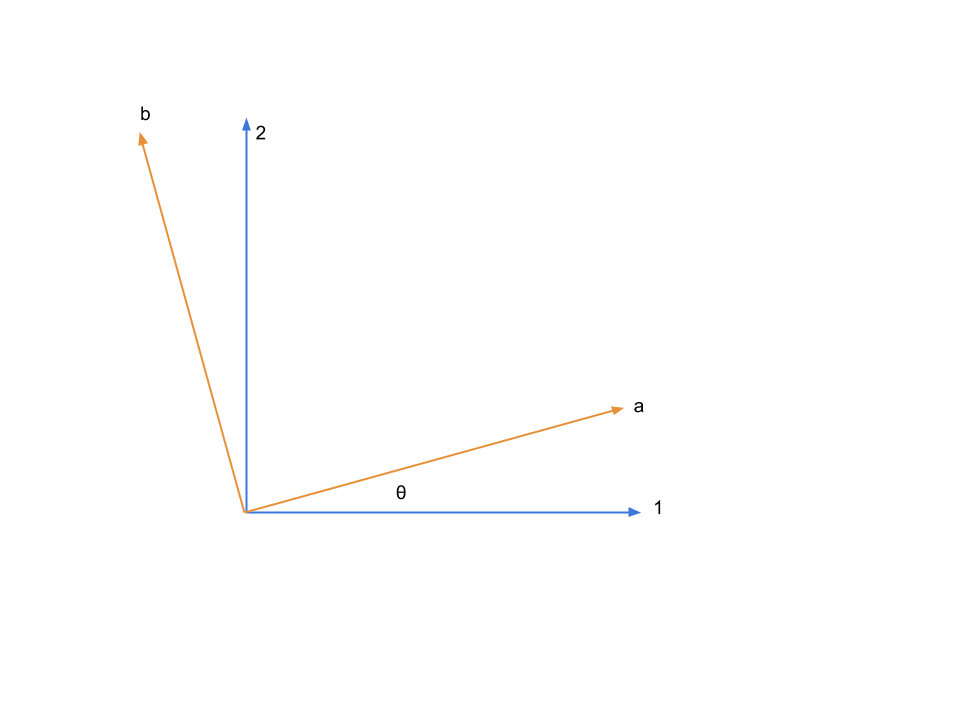
\includegraphics{nuetrinoMixingAngle.png}
\caption{Two flavour neutrino mixing diagram with \(\theta\) being the mixing angle}\end{figure}

The flavour states can be expressed in terms of mass eigenstates,
\begin{gather}
\begin{split}\begin{pmatrix}\nu_a \\ \nu_b\end{pmatrix} = \begin{pmatrix}  \cos\theta  & \sin\theta \\ -\sin\theta  & \cos\theta \end{pmatrix}   \begin{pmatrix}\nu_1 \\ \nu_2\end{pmatrix}\end{split}\notag
\end{gather}
where the matrix
\begin{gather}
\begin{split}\mathbf U = \begin{pmatrix}  \cos\theta  &  \sin\theta \\ -\sin\theta  & \cos\theta \end{pmatrix}\end{split}\notag
\end{gather}
is the mixing matrix which is a rotation of basis geometrically. In other words, this matrix is the representation of the rotation \(e^{i\hat\theta}\).


\subsubsection{Survival Probability}
\label{oscillations:survival-probability}
Neutrinos are usually produced in electron flavor, which we choose as the initial condition for this example,
\begin{gather}
\begin{split}\ket{\psi(t=0)} = \cos\theta \ket{\nu_1} + \sin \theta \ket{\nu_2}.\end{split}\notag
\end{gather}
With the mixing matrix, the propagation of an initial state of only flavour a is
\begin{gather}
\begin{split}\ket{\psi(t)} = \cos\theta \ket{\nu_1} e^{-i E_1 t} + \sin\theta \ket{\nu_2} e^{-i E_2 t} .\end{split}\notag
\end{gather}
To find out the amplitude of flavour a, we need to project the state \(\ket{\psi(t)}\) onto a flavour eigenstate, say, \(\ket{\nu_a}\),
\begin{gather}
\begin{split}\braket{\nu_a}{\psi(t)} & = \bra{\nu_a}\left( \cos\theta \ket{\nu_1} e^{-i E_1 t} + \sin\theta \ket{\nu_2} e^{-i E_2 t}\right) \\
&= \left( \cos\theta \ket{\nu_1}  + \sin\theta \ket{\nu_2} \right) \left( \cos\theta \ket{\nu_1} e^{-i E_1 t} + \sin\theta \ket{\nu_2} e^{-i E_2 t}\right) \\
& = \cos^2\theta e^{-iE_1t} + \sin^2\theta e^{-i E_2 t}\end{split}\notag
\end{gather}
The survival probability is the amplitude squared,
\begin{gather}
\begin{split}P_{aa} & = \lvert \braket{\nu_a}{\psi(t)} \rvert ^2 \\
& = \lvert \cos^2\theta e^{-iE_1t} + \sin^2\theta e^{-i E_2 t}  \rvert^2 \\
& = \left( \cos^2\theta e^{-iE_1t} + \sin^2\theta e^{-i E_2 t}  \right)^* \left( \cos^2\theta e^{-iE_1t} + \sin^2\theta e^{-i E_2 t}  \right) \\
& = \cos^4\theta + \sin^4\theta + \cos^2\theta\sin^2\theta e^{i(E_1-E_2)t}+ \sin^2\theta\cos^2\theta e^{-i(E_1-E_2)t} \\
& = \cos^4\theta + \sin^4\theta + \cos^2\theta\sin^2\theta e^{i\Delta E t}+ \sin^2\theta\cos^2\theta e^{-i\Delta E t} \\
& = \cos^4\theta + \sin^4\theta + 2 \cos^2\theta\sin^2\theta \cos(\Delta E t) \\
& = (\cos^2\theta +\sin^2\theta)^2 - 2\cos^2\theta \sin^2\theta  + 2 \cos^2\theta\sin^2\theta \cos(\Delta E t) \\
& = 1 - 2 \cos^2\theta \sin^2\theta (1 - \cos(\Delta E t)) \\
& = 1 - \sin^2(2\theta) \sin^2\left( \frac{\Delta E t}{2} \right)\end{split}\notag
\end{gather}
with the definition \(\Delta E =  E_1-E_2 \approx p_1 + \frac{1}{2}\frac{m_1^2}{p_1} - p_2 - \frac{1}{2}\frac{m_2^2}{p_2}\). We usually calculate the case \(p_1=p_2=p\) , which takes us to
\begin{gather}
\begin{split}\Delta E & \approx \frac{m_1^2 - m_2^2}{2p} \\
& = \frac{\delta^2 m}{2p} .\end{split}\notag
\end{gather}
with \(\delta^2 m=m_1^2 - m_2^2\). Most of the time we would like to know the oscillation with respect to distance. Using the approximation \(t = L\) and \(\Delta E \approx \frac{m_1^2 - m_2^2}{2p}\), we have
\begin{gather}
\begin{split}P_{aa} &= 1 - \sin^2(2\theta) \sin^2\left( \frac{\Delta E L}{2} \right) \\
& = 1 -  \sin^2(2\theta) \sin^2\left( \frac{ \delta m^2  L}{4p} \right) .\end{split}\notag
\end{gather}
This is the survival probability of flavour a neutrino with an initial state of flavour a.

There are several things to be noticed,
\begin{enumerate}
\item {} 
\(\theta=0\) leads to oscillation free neutrinos.

\item {} 
\(\Delta E=0\) or \(\delta ^2m =0\) (in the case of same momentum) also gives us no oscillation.

\item {} 
At \(L=0\) the survival probability is 1, which means no oscillation is done.

\end{enumerate}


\subsubsection{Hamiltonian}
\label{oscillations:hamiltonian}
It's easy to write down the Hamiltonian for the mass state stationary Schrodinger equation. As we have proven, to first order approximation,
\begin{gather}
\begin{split}E = p + \frac{1}{2}\frac{m^2}{p}\end{split}\notag
\end{gather}\begin{gather}
\begin{split}\mathbf H_j &= \begin{pmatrix} p + \frac{1}{2}\frac{m_1^2}{p} & 0 \\ 0 & p + \frac{1}{2}\frac{m_2^2}{p} \end{pmatrix} \\
& = p \mathbf I + \frac{1}{2p}\begin{pmatrix} m_1^2 & 0 \\ 0 & m_2^2 \end{pmatrix}\end{split}\notag
\end{gather}
However, the Hamiltonian we prefer is the one for flavour eigenstates. To achieve this, we only need to rotate this previous Hamiltonian using the mixing matrix \(\mathbf U\).
\begin{gather}
\begin{split}\mathbf H_{\alpha} & = \mathbf U \hat H_j  \mathbf U^T \\
& =  \begin{pmatrix}  \cos\theta & \sin\theta \\ -\sin\theta  & \cos\theta \end{pmatrix} \left( p \mathbf I + \frac{1}{2p}\begin{pmatrix} m_1^2 & 0 \\ 0 & m_2^2 \end{pmatrix} \right)   \begin{pmatrix}  \cos\theta & -\sin\theta \\ \sin\theta & \cos\theta \end{pmatrix} \\
& = p \mathbf I + \frac{1}{2p} \begin{pmatrix} \cos^2\theta m_1^2 + \sin^2\theta m_2^2 & -\sin\theta\cos\theta m_1^2 + \sin\theta\cos\theta m_2^2 \\ -\sin\theta\cos\theta m_1^2 + \sin\theta\cos\theta m_2^2 & \sin^2\theta m_1^2 + \cos^2\theta m_2^2 \end{pmatrix} \\
& = p \mathbf I + \frac{1}{2p} \begin{pmatrix} m_1^2 - \delta^2 m \sin^2\theta & -\frac{1}{2}\sin 2\theta  \delta m^2  \\ -\frac{1}{2}\sin 2\theta  \delta m^2  & m_2^2+ \delta m^2 \sin^2\theta \end{pmatrix} \\
& = p \mathbf I + \frac{1}{2p} \left( \frac{1}{2}(m_1^2+m_2^2) \mathbf I -   \frac{1}{2}\begin{pmatrix} - \delta m^2 \cos 2\theta & \delta^2 m \sin 2\theta \\  \delta m^2 \sin 2\theta & \delta^2 m\cos 2\theta \end{pmatrix} \right) \\
& = \left(p + \frac{m_1^2+m_2^2}{4p} \right)\mathbf I - \frac{1}{4p}\begin{pmatrix} - \delta m^2 \cos 2\theta & \delta^2 m \sin 2\theta \\  \delta m^2 \sin 2\theta & \delta^2 m\cos 2\theta \end{pmatrix}\end{split}\notag
\end{gather}
Again we see clearly, no oscillation will apear as long as mixing angle \(\theta=0\) or \(\delta m^2 =0\).

\begin{notice}{note}{Note:}
The reason we can do this is that this mixing matrix is time and space independent. To see this, we first write down the Schrodinger equation for mass eigenstates,
\begin{gather}
\begin{split}i d_t \ket{\Phi_j} = \hat H_j \ket{\Phi_j}.\end{split}\notag
\end{gather}
Applying the mixing matrix,
\begin{gather}
\begin{split}i d_t \mathbf U^{-1} \ket{\Phi_\alpha} = \hat H_j  \mathbf U^{-1} \ket{\Phi_\alpha}.\end{split}\notag
\end{gather}
Notice that the mixing matrix, which is a rotation, is orthonormal, \(\mathbf U \mathbf U^T=\mathbf I\). Then we have inverse of this matrix is the same as the transpose.
\begin{gather}
\begin{split}i d_t \mathbf U^T \ket{\Phi_\alpha} = \hat H_j  \mathbf U^T \ket{\Phi_\alpha}.\end{split}\notag
\end{gather}
Multiply on both sides \(\mathbf U\) and remember the fact that the mixing matrix is orthonormal, we have
\begin{gather}
\begin{split}i d_t \ket{\Phi_\alpha} = \mathbf U \hat H_j  \mathbf U^T \ket{\Phi_\alpha}.\end{split}\notag
\end{gather}
Now we can define the Hamiltonian for flavour states,
\begin{gather}
\begin{split}\mathbf H_{\alpha} = \mathbf U \mathbf H_j  \mathbf U^T .\end{split}\notag
\end{gather}\end{notice}

Since Pauli matrices plus identity forms a complete basis for all 2 by 2 matrices, it our Hamiltonian can be written as
\begin{gather}
\begin{split}\mathbf H  &= \frac{\delta^2 m}{4E}\begin{pmatrix} -\cos 2\theta & \sin 2\theta \\ \sin 2\theta & \cos 2\theta \end{pmatrix} \\
& = \frac{\delta^2 m}{4 E} \left( -\cos 2\theta \mathbf{\sigma_z} + \sin 2\theta \mathbf{\sigma_x} \right).\end{split}\notag
\end{gather}
\begin{notice}{note}{Note:}
Pauli matrices are
\begin{gather}
\begin{split}\sigma_x = \begin{pmatrix}0 & 1 \\ 1 & 0\end{pmatrix} \\
\sigma_y = \begin{pmatrix}0 & -i \\ i & 0\end{pmatrix} \\
\sigma_x = \begin{pmatrix}1 & 0 \\ 0 & -1\end{pmatrix}.\end{split}\notag
\end{gather}
In a more compact way,
\begin{gather}
\begin{split}\sigma_j = \begin{pmatrix} \delta_{j3}&\delta_{j1}-i\delta_{j2}\\ \delta_{j1}+i\delta_{j2}&-\delta_{j3}\end{pmatrix}  .\end{split}\notag
\end{gather}\end{notice}


\section{Equation of Motion in Matter}
\label{oscillations:equation-of-motion-in-matter}

\subsection{Hamiltonian}
\label{oscillations:id3}
We have already derived the Hamiltonian for vacuum oscillatioin,
\begin{gather}
\begin{split}H_v=\frac{ \delta m^2 }{2E}\frac{1}{2}\begin{pmatrix} -\cos 2\theta_v & \sin 2 \theta_v \\ \sin 2\theta_v & \cos 2\theta_v  \end{pmatrix},\end{split}\notag
\end{gather}
where we would like to define a new matrix,
\begin{gather}
\begin{split}\mathbf B = \frac{1}{2}\begin{pmatrix}  -\cos 2\theta_v & \sin 2 \theta_v \\ \sin 2\theta_v & \cos 2\theta_v  \end{pmatrix},\end{split}\notag
\end{gather}
so that the vacuum Hamiltonian can be written as
\begin{gather}
\begin{split}H_v = \frac{ \delta m^2 }{2E}\mathbf B\end{split}\notag
\end{gather}
The \textbf{effect of matter}, as we have already discussed before, adds an extra term
\begin{gather}
\begin{split}H_m = \sqrt{2}G_F n_e L.\end{split}\notag
\end{gather}
Here we have
\begin{gather}
\begin{split}L = \begin{pmatrix} 1 & 0 \\ 0 & 0 \end{pmatrix}.\end{split}\notag
\end{gather}
\begin{notice}{note}{Note:}
Previously in the MSW effect section, we have \(L=\frac{1}{2}\sigma_3\). The reason, as explained there, is that we can always write down a 2 by 2 matrix using Pauli matrices and indentity matrix and identity matrix only shifts the overall eigenvalue not the eigenvector so we can just drop the identity term.
\end{notice}

One other term is the self-interaction of neutrinos, i.e., neutral-current neutrino-neutrino forward exchange scattering,
\begin{gather}
\begin{split}H_\nu =\sqrt{2}G_F \int d^3\mathbf p' (1-\hat {\mathbf p}\cdot \hat{\mathbf p}')(\rho_{p'}-\bar \rho_{p'}).\end{split}\notag
\end{gather}
The overall Hamiltonian is
\begin{gather}
\begin{split}H = H_0 + H_m + H_\nu ,\end{split}\notag
\end{gather}
where the vacuum Hamiltonian is
\begin{gather}
\begin{split}H_0 &= \frac{\delta^2 m}{2E} \mathbf B \\
& = \frac{\delta^2 m}{2E} U \left(\frac{1}{2}\sigma_3 \right) U^\dagger .\end{split}\notag
\end{gather}

\subsection{Equation of Motion}
\label{oscillations:equation-of-motion}
From the Hamiltonian, Von Neumann equation is
\begin{gather}
\begin{split}i \frac{\partial}{\partial t}\rho = \left[ H , \rho\right]\end{split}\notag
\end{gather}
In Picture chapter we have seen the definition of a polarization matrix. The components of a polarization vector (\textbf{for neutrinos}) is given by
\begin{gather}
\begin{split}P_{\omega,i} &\propto \mathrm{Tr} (\rho_E \sigma_i) \\
& = \frac{1}{n_\nu} \frac{\lvert \delta^2 m \rvert}{2\omega^2} \times  \mathrm{Tr} (\rho_E \sigma_i) .\end{split}\notag
\end{gather}
For anitneutrinos, we have a negative \(\omega\) which is defined as \(\omega = \frac{ \delta m^2 }{2E}\) (neutrinos) and \(\omega_{\bar\nu}= - \frac{ \delta m^2 }{2E}\) (anitneutrinos). The polarization is defined as
\begin{gather}
\begin{split}P_{\omega,i} = - \frac{1}{n_\nu} \frac{\lvert \delta^2 m \rvert}{2\omega^2} \times  \mathrm{Tr} (\bar \rho_E \sigma_i) .\end{split}\notag
\end{gather}
With all these definitions, Von Neumann equation multiply by \(\vec{\sigma} = \sigma_1 \hat e_1 + \sigma_2 \hat e_2 + \sigma_3 \hat e_3\), we have
\begin{gather}
\begin{split}i \dot \rho \sum_i \sigma_i \hat e_i = \left[H, \rho\right] \sum_i\sigma_i \hat e_i.\end{split}\notag
\end{gather}
Notice that Pauli matrices are Hermitian and Unitary, we can alway insert the identity \(\mathbf I = \sigma_j \sigma_j^\dagger\).

\begin{notice}{note}{Commutator and Cross Product}

Commutator of two vectors,
\begin{gather}
\begin{split}\vec A \times \vec B & = (A_2 B_3 - A_3 B_2) \hat e_1 + (A_3 B_1 - A_1 B_2)\hat e_2 + (A_1 B_2 - A_2 B_3)\hat e_3\end{split}\notag
\end{gather}\end{notice}

\begin{notice}{note}{Trace of Pauli Matrices}

All Pauli matrices have vanishing trace. And what makes our calculation more convinient is that the trace of matrices is invariant under cyclic permutation, that is
\begin{gather}
\begin{split}\mathrm{Tr}(\sigma_i \mathbf H \sigma_j) = \mathrm{Tr}(\mathbf H \sigma_j\sigma_i)\end{split}\notag
\end{gather}
Notice that to have a non-vanishing trace we need \(i=j\). This property really saves our life.
\end{notice}

As the definition, we have
\begin{gather}
\begin{split}\mathbf H &= \vec H\cdot \vec\sigma \\
\rho & = \vec \rho \cdot \vec \sigma\end{split}\notag
\end{gather}
Using these we can rewrite the commutator
\begin{gather}
\begin{split}[H,\rho] & = [\vec H \cdot \vec\sigma, \vec \rho \cdot \vec \sigma] \\
& = \sum_{ik}(H_i \sigma_i \rho_k \sigma_k - \rho_k \sigma_k H_i \sigma_i )\\
& = \sum_{ik}(H_i\rho_k \sigma_i\sigma_k - \rho_k H_i \sigma_k \sigma_i) \\
& = \sum_{ik} H_i\rho_k (\sigma_i\sigma_k-\sigma_k\sigma_i) \\
& = \sum_{ik} H_i \rho_k [\sigma_i,\sigma_k] \\
& =  \sum_{ik} H_i \rho_k 2i \epsilon_{ikn}\sigma_n \\
& =  2i \sum_{ik}\epsilon_{ikn}\sigma_n H_i \rho_k\end{split}\notag
\end{gather}
Multiply by \(\sigma_j\) and take the trace, we get,
\begin{gather}
\begin{split}\mathrm{Tr}(\sigma_j [H,\rho]) & =  2i \mathrm{Tr}(\sum_{ik}\epsilon_{ikn}\sigma_j\sigma_n H_i \rho_k )\\
&= 2i \sum_{ik} \mathrm{Tr}(\epsilon_{ikj} \mathrm I  H_i \rho_k  ) \\
& = 2i \sum_{ik} \epsilon_{jik} H_i\rho_k  \mathrm{Tr}(\mathbf I) \\
& = 4i \epsilon_{jik}H_i\rho_k.\end{split}\notag
\end{gather}
The corresponding LHS after these work becomes
\begin{gather}
\begin{split}i\mathrm{Tr}(\sigma_j \dot \rho_i \sigma_i) & = i \partial_t \rho_j \mathrm{Tr}( I) \\
& = 2i\dot{P_j}\end{split}\notag
\end{gather}
The Von Neuman equation becomes
\begin{gather}
\begin{split}\dot{\vec P} = 2 \vec H \times \vec P.\end{split}\notag
\end{gather}
We know explicitly what polarization vector is
\begin{gather}
\begin{split}P_j = \mathrm{Constant} \mathrm {Tr} (\rho \sigma_j)\end{split}\notag
\end{gather}
for neutrinos while
\begin{gather}
\begin{split}\bar P_j = -\mathrm{Constant} \mathrm {Tr} (\bar \rho \sigma_j).\end{split}\notag
\end{gather}
The vectorized Hamiltonian is
\begin{gather}
\begin{split}H = H_i\sigma_i.\end{split}\notag
\end{gather}
Multiply by \(\sigma_j\) and take the trace,
\begin{gather}
\begin{split}\mathrm{Tr}(H\sigma_j) = H_j \mathrm{Tr}(\mathbf I),\end{split}\notag
\end{gather}
that is,
\begin{gather}
\begin{split}\mathrm{Tr}(H\sigma_j) = 2 H_j.\end{split}\notag
\end{gather}
\begin{notice}{note}{Hamiltonian}

The Hamiltonian for homogeneous isotropic environment is
\begin{gather}
\begin{split}H &= H_0 + H_m + H_\nu \\
& = \omega \mathbf B + \lambda \mathbf L + \sqrt{ G_F} \int_0^\infty dE' (\rho_E' - \bar \rho_E' ).\end{split}\notag
\end{gather}\end{notice}

Then the equation we need becomes
\begin{gather}
\begin{split}\dot{\vec P_\omega} = (\omega \vec B + \lambda \vec L + \mu \vec D) \times \vec P_{\omega}.\end{split}\notag
\end{gather}
where \(\vec B = \mathrm {Tr}(\mathbf B \vec \sigma)\), \(\vec L = \mathrm{Tr}(\mathbf L \vec \sigma)\), \(\vec D = \int_{-\infty}^{\infty}d\omega \vec P_\omega\).


\section{Q\&A}
\label{oscillations:q-a}
\begin{notice}{note}{Question}

What are some of the conventions used in liturature?
\end{notice}

\begin{notice}{note}{Answer}
\begin{enumerate}
\item {} 
\(\Delta m^2_{ij}=m_i^2-m_j^2\).

\item {} 
Flavours of left hand neutrinos are mixing of mass eigen states, \(\nu_{lL}=\sum_{j=1}^3 U_{lj}\nu_{jL}(x)\).

\end{enumerate}
\end{notice}

\begin{notice}{note}{Question}

Why can we use just quantum mechanics on relativistic neutrinos? In principle one should use quantum field theory or at least relativistic quantum mechanics?
\end{notice}

\begin{notice}{note}{Answer}

To be answered.
\end{notice}

\begin{notice}{note}{Question}

What does the mixing angle mean exactly both in vacuum and matter environment?
\end{notice}

\begin{notice}{note}{Answer}

There are several ways to illustrate this.
\begin{enumerate}
\item {} 
\textbf{Rotation angle} in flavour space. For simplicity I use a two component neutrino model.

\end{enumerate}
\begin{gather}
\begin{split}\ket{\nu_1} &= \cos\theta \ket{\nu_e} + \sin \theta \ket{\nu_\mu} \\
\ket{\nu_2} & = -\sin\theta \ket{\nu_e} + \cos\theta \ket{\nu_\mu}\end{split}\notag
\end{gather}
This is a rotation in a plane with a generator \(e^{-i\hat \theta}\). \textbf{(Make a figure for this.) + (Write down the 3 components model.)}
\begin{enumerate}
\setcounter{enumi}{1}
\item {} 
\textbf{Oscillation probability} involves this angle too. It is a suppression of the oscillation probability.

\item {} 
From the view of \textbf{quantum states}, this angle determines how the flavour states are composed with mass eigenstates, i.e., the fraction or probability of each mass eiginstates in a flavour state.

\end{enumerate}
\end{notice}

\begin{notice}{note}{Question}

What does wave packet in neutrino oscillation mean?
\end{notice}

\begin{notice}{note}{Answer}

To Be Answered.
\end{notice}

\begin{notice}{note}{Question}

How would a wave packet spread?
\end{notice}

\begin{notice}{note}{Answer}

A Gaussian wave packet would spread or shrink. The key of this spreading or shrinking is the dispersion relation.

For \textbf{non-relativistic} Gaussian wave packet \(\psi(x,t) = e^{-\alpha(k-k_0)^2}\) in momentum basis with dispersion relation \(\hbar\omega = \frac{\hbar^2 k^2}{2m}\), the expansion of packet is
\begin{gather}
\begin{split}\Delta x= \sqrt{\alpha^2+\left(\frac{\hbar t}{2m}\right)^2} .\end{split}\notag
\end{gather}
Obviously, the RMS width spreads according to group velocity \(v_g = \hbar _0/m\).

\textbf{However, the situation could be different for a relativistic neutrino.}
\end{notice}

\begin{notice}{note}{Question}

What will scattering do to a wave packet.
\end{notice}

\begin{notice}{note}{Answer}

\textbf{Momentum transfer} for a plan wave case in Born approximation is
\end{notice}


\section{Refs \& Notes}
\label{oscillations:refs-notes}

\chapter{Vacuum Oscillation}
\label{vacuum:vacuum-oscillation}\label{vacuum::doc}
Schrodinger equation is
\begin{gather}
\begin{split}i\partial_t \ket{\Psi} = \mathbf H \ket{\Psi},\end{split}\notag
\end{gather}
where for relativistic neutrinos, the energy is
\begin{gather}
\begin{split}\mathbf H^{vm} &= \begin{pmatrix}\sqrt{p^2 + m_1^2} & 0 & 0 \\ 0& \sqrt{p^2 + m_2^2} & 0 \\ 0 & 0 & \sqrt{p^2 + m_3^2}  \end{pmatrix},\end{split}\notag
\end{gather}
in which the energy terms are simplified using the relativistic condition
\begin{gather}
\begin{split}\sqrt{p^2+m_i^2} & = p\sqrt{1 + \frac{m_i^2}{p^2}} \\
&\approx  p(1 + \frac{1}{2} \frac{m_i^2}{p^2}).\end{split}\notag
\end{gather}
\begin{notice}{note}{So Called Decoherence}

Here we assume that they all have the same energy but different mass. The thing is we assume they have the same velocity since the mass is very small. To have an idea of the velocity difference, we can calculate the distance travelled by another neutrino in the frame of one neutrino.

Assuming the mass of a neutrino is 1eV with energy 10MeV, we will get a speed of \(1-10^{-14}\) c. This \(10^{-14}\) c will make a difference about \(3\mu\mathrm{ m}\) in 1s.

Will decoherence happen due to this? For high energy neutrinos this won't be a problem however for low energy neutrinos this will definitely cause a problem for the wave function approach.Because the different mass eigenstates will become decoherent gradually along the path.

A estimation of the decoherence length is
\begin{gather}
\begin{split}l_{\mathrm{coh}}=\frac{v_g}{\Delta v_g}\sigma.\end{split}\notag
\end{gather}
To obtain the relation,
\begin{gather}
\begin{split}\Delta x &= \lvert v_1 - v_2 \rvert t_{\mathrm{coh}}\\
\frac{\hbar c}{\Delta E} & = \lvert \frac{m_1^2}{2E_1^2} - \frac{m_2^2}{2E_2^2} \rvert t_{\mathrm{coh}} \\
\frac{\hbar c}{\Delta E} & = \frac{1}{2E}\lvert \Delta m_{12}^2 \rvert t_{\mathrm{coh}}\end{split}\notag
\end{gather}
\textbf{It should be made clear that this is not really decoherence but in the view of wave packet formalism different propagation eigenstates will be far away from each other. As long as we put them together again we can overlap and oscillate again. No quantum decoherence is happening at all.}
\end{notice}

In general the flavor eigenstates are the mixing of the mass eigenstates with a unitary matrix \(\mathbf U\), that is
\begin{gather}
\begin{split}\ket{\nu_{\alpha}} =  U_{\alpha i} \ket{\nu_i},\end{split}\notag
\end{gather}
where the \(\alpha\) s are indices for flavor states while the \emph{i} s are indices for mass eigenstates.

To find out the equation of motion for flavor states, plugin in the initary tranformation,
\begin{gather}
\begin{split}i  U_{\alpha i} \partial_t \ket{\nu_i} =  U_{\alpha i}  H^m_{ij} \ket{\nu_j}.\end{split}\notag
\end{gather}
We use index \({}^{vm}\) for representation of Hamiltonian in mass eigenstates in vacuum oscillations. Applying the unitary condition of the transformation,
\begin{gather}
\begin{split}\mathbf I = \mathbf {U^\dagger} \mathbf U,\end{split}\notag
\end{gather}
I get
\begin{gather}
\begin{split}i U_{\alpha i} \partial_t \ket{\nu_i} =  U_{\alpha i} H^m_{i j}  {U^\dagger_{j\beta}}  U_{\beta k} \ket{\nu_k},\end{split}\notag
\end{gather}
which is simplified to
\begin{gather}
\begin{split}i \partial_t \ket{\nu_\alpha} = H^f_{\alpha \beta} \ket{\nu_{\beta}},\end{split}\notag
\end{gather}
since the transformation is time independent.

The new Hamiltonian in the representations of flavor eigenstates reads
\begin{gather}
\begin{split}H^f_{\alpha\beta}  = U^\dagger_{\alpha i} H^m_{ij} U_{j\beta}.\end{split}\notag
\end{gather}

\section{Survival Problem}
\label{vacuum:survival-problem}
The neutrino states at any time can be written as
\begin{gather}
\begin{split}\ket{\Psi(t)}  = X_1 \ket{\nu_1 } e^{-i E_1 t}+ X_2 \ket{ \nu_2 } e^{-i E_2 t},\end{split}\notag
\end{gather}
where \(X_1\) and \(X_2\) are the initial conditions which are determined using the neutrino initial states.

Survival probalility is the squrare of the projection on an flavor eigenstate,
\begin{gather}
\begin{split}P_{\alpha}(t) = \lvert \braket{\nu_{\alpha}}{\Psi(t)} \rvert^2.\end{split}\notag
\end{gather}
The calculation of this expression requires our knowledge of the relation between mass eigenstates and flavor eigenstates which we have already found out.

Recall that the transformation between flavor and mass states is
\begin{gather}
\begin{split}\ket{\nu_i} = U^{-1}_{i\alpha} \ket{\nu_\alpha},\end{split}\notag
\end{gather}
which leads to the inner product of mass eigenstates and flavor eigenstates,
\begin{gather}
\begin{split}\braket{\nu_\alpha}{\nu_i} &= \bra{\nu_\alpha} U^{-1}_{i\beta} \ket{\nu_\beta} \\
& = U^{-1}_{i\beta}\delta_{\alpha\beta} \\
& = U^{-1}_{i\alpha}.\end{split}\notag
\end{gather}
The survival probability becomes
\begin{gather}
\begin{split}P_\alpha (t) &= \lvert \braket{\nu_\alpha}{ X_1 \ket{\nu_1 } e^{-i E_1 t} X_2 \ket{ \nu_2 } e^{-i E_2 t} }  \rvert^2 \\
& = \lvert  X_1 e^{-i E_1 t} \braket{\nu_\alpha}{\ket{\nu_1} } + X_2 e^{-i E_2 t} \braket{ \nu_\alpha }{ \nu_2 } \rvert^2 \\
& = \lvert \sum_i X_i e^{-i E_i t} U^{-1}_{i \alpha}  \rvert ^2 \\
& = \sum_i X_1^* e^{iE_i t} U^{\dagger *}_{i\alpha} \sum_i X_i e^{-i E_i t} U^\dagger_{i \alpha} \\
& = \lvert X_1 \rvert^2 U^{\dagger * } _ {1\alpha} U^\dagger_{1\alpha} + \lvert X_2 \rvert^2 U^{\dagger * } _ {2\alpha} U^\dagger_{2\alpha}  + X_1^* X_2 U^{\dagger * }_{1\alpha} U^\dagger_{2\alpha} e^{i E_1 t - i E_2 t} + X_2^* X_1 U^{\dagger * }_{2\alpha} U^\dagger_{1\alpha} e^{i E_2 t - i E_1 t}\end{split}\notag
\end{gather}
\(U^{\dagger *}_{i\alpha}\) stands for the \emph{i} th row and the \(\alpha\) th column of the matrix \(U^{\dagger *}\).


\section{Two Flavor States}
\label{vacuum:two-flavor-states}
Suppose the neutrinos are prepared in electron flavor initially, the survival probability of electron flavor neutrinos is calculated using the result I get previously.

Electron neutrinos are the lighter ones, then I have \({}_a = {}_e\) and denote \({}_b={}_x\).

\begin{notice}{note}{Meaning of Mixing}

In the small mixing angle limit,
\begin{gather}
\begin{split}\begin{pmatrix}\nu_e \\ \nu_x\end{pmatrix} \to \begin{pmatrix}  1 & \theta \\ -\theta  & 1 \end{pmatrix}   \begin{pmatrix}\nu_1 \\ \nu_2\end{pmatrix}\end{split}\notag
\end{gather}
which is very close to an identity matrix. This implies that electron neutrino is more like mass eigenstate  \(\nu_1\) . By \(\nu_1\) we mean the state with energy  \(\frac{ \delta m^2 }{4E}\) in vacuum.
\end{notice}

In fact the dynamics of the system is very easily solved without dive into the math. Suppose we have \(\ket{\nu_e}\) initially, which is
\begin{gather}
\begin{split}\Psi(x=0)=\ket{\nu_e} = \cos \theta_v \ket{\nu_1} - \sin \theta_v \ket{\nu_2},\end{split}\notag
\end{gather}
the state of the system at distance \(x\) is directly written down
\begin{gather}
\begin{split}\Psi(x) &=  \cos \theta_v \ket{\nu_1} e^{-i E_1 x} - \sin \theta_v \ket{\nu_2} e^{-i E_2 x} \\
&= e^{-i E_1 x}( \cos \theta_v \ket{\nu_1}  - \sin \theta_v \ket{\nu_2} e^{i(E_1 - E_2) x}).\end{split}\notag
\end{gather}
Since a global phase doesn't change the detection, we write the state as
\begin{gather}
\begin{split}\Psi(x) =  \cos \theta_v \ket{\nu_1}  - \sin \theta_v \ket{\nu_2} e^{i(E_1 - E_2) x} .\end{split}\notag
\end{gather}
Notice that the period of the expression is
\begin{gather}
\begin{split}l_v = \frac{2\pi}{E_1 - E_2} = - \frac{4\pi E}{\Delta m_{12}}.\end{split}\notag
\end{gather}
Recall the definition of angular frequency in vacuum \(\omega = \frac{\Delta m^2}{2E}\). The relation between period and angular frequency is indeed \(\omega = \frac{2\pi}{l_v}\) as we should have been defined them.

Then the state becomes
\begin{gather}
\begin{split}\Psi(x) =  \cos \theta_v \ket{\nu_1}  - \sin \theta_v \ket{\nu_2} e^{i2\pi x/l_v} .\end{split}\notag
\end{gather}
The survival probability for electron neutrinos is
\begin{gather}
\begin{split}P(\nu_e,L) &= 1-\sin^2(2\theta_v)\sin^2\left( \frac{\Delta m^2 L}{4E} \right) \\
&= 1- \frac{1}{2}\sin^2 2\theta_v \left(1- \cos\left( \frac{2\pi x}{l_v} \right) \right)\end{split}\notag
\end{gather}

\section{The Standard Math for 2 Flavor Neutrino}
\label{vacuum:the-standard-math-for-2-flavor-neutrino}
\textbf{This section is to demonstrate the standard math for differential equations we have learned in first year undergrad. In fact almost all the procedures are not necessary because we get this Hamiltonian in Flavor basis by transform the diagonalized Hamiltonian in mass eigenstates basis using the mixing matrix. Hence this section only works as a review of mathematics.}

To solve a set of first order differential equations, I need the determinant of coefficient matrix. For 2 flavor neutrino oscillations, the equation of motion is
\begin{gather}
\begin{split}\partial_x \begin{pmatrix}
\nu_e(x) \\ \nu_x(x)
\end{pmatrix} = i \frac{\omega}{2} \begin{pmatrix}
-\cos 2\theta_v &    \sin 2\theta_v \\   \sin 2\theta_v & \cos 2\theta_v
\end{pmatrix} \begin{pmatrix}
\nu_e(x) \\ \nu_x(t)
\end{pmatrix}.\end{split}\notag
\end{gather}
To find the solutions I need the eigenvalues \(\lambda\) . The determinant of the Hamiltonian is
\begin{gather}
\begin{split}&\det \left(  i\frac{\omega}{2} \begin{pmatrix}
-\cos 2\theta_v &    \sin 2\theta_v \\   \sin 2\theta_v &  \cos 2\theta_v
\end{pmatrix} - \lambda \mathbf{I} \right) \\
=& \begin{vmatrix}
-i \frac{\omega}{2} \cos 2\theta_v - \lambda & i \frac{\omega}{2} \sin 2\theta_v \\
i \frac{\omega}{2} \sin 2\theta_v & i \frac{\omega}{2} \cos 2\theta_v - \lambda
\end{vmatrix} .\end{split}\notag
\end{gather}
By defining \(\lambda' = \lambda/(-i \omega / 2)\), the determinant is
\begin{gather}
\begin{split}- \left( \frac{\omega}{2} \right)^2   ( (\cos 2\theta_v - \lambda')(-\cos 2\theta_v - \lambda') - \sin 2\theta_v \sin 2\theta_v ) .\end{split}\notag
\end{gather}
The eigenvalues are the solutions to
\begin{gather}
\begin{split}- \left( \frac{\omega}{2} \right)^2   ( (\cos 2\theta_v - \lambda')(-\cos 2\theta_v - \lambda') - \sin^2 2\theta_v  ) =0 ,\end{split}\notag
\end{gather}
whose solution is
\begin{gather}
\begin{split}\lambda' = \pm 1.\end{split}\notag
\end{gather}
With the solutions
\begin{gather}
\begin{split}\lambda = \pm i \frac{\omega}{2},\end{split}\notag
\end{gather}
the eigenvectors can also be solved.
\begin{gather}
\begin{split}\begin{pmatrix}
\cos 2\theta_v - 1 &  -  \sin 2\theta_v \\  - \sin 2\theta_v & - \cos 2\theta_v -1
\end{pmatrix} \begin{pmatrix}
\eta_1 \\ \eta_2
\end{pmatrix} = \begin{pmatrix}
0 \\ 0
\end{pmatrix}\end{split}\notag
\end{gather}
gives us \(\eta_2 = -\tan \theta_v \eta_1\), which means the eigenvectors are
\begin{gather}
\begin{split}\begin{pmatrix}
1  \\ -\tan\theta_v
\end{pmatrix} , \begin{pmatrix}
1 \\ \cot \theta_v
\end{pmatrix}.\end{split}\notag
\end{gather}
The general solution of the first order differential equations is
\begin{gather}
\begin{split}\begin{pmatrix}
1 \\ -\tan\theta_v
\end{pmatrix} e^{-i \omega x/ 2 } \\
\begin{pmatrix}
1 \\ \cot \theta_v
\end{pmatrix} e^{i  \omega x/ 2 }.\end{split}\notag
\end{gather}
Initial condition is
\begin{gather}
\begin{split}\begin{pmatrix}
1 \\ 0
\end{pmatrix},\end{split}\notag
\end{gather}
and it determines the final solution
\begin{gather}
\begin{split}& \cos^2\theta \begin{pmatrix}
1 \\ -\tan\theta_v
\end{pmatrix} e^{-i \omega x/ 2 } + \sin^2\theta_v
\begin{pmatrix}
1 \\ \cot \theta
\end{pmatrix} e^{i  \omega x/ 2 } \\
= & \begin{pmatrix}
\cos^2\theta_v \\ -\sin\theta_v \cos\theta_v
\end{pmatrix} e^{-i \omega x/ 2 } +
\begin{pmatrix}
\sin^2\theta_v \\ \sin\theta_v \cos \theta_v
\end{pmatrix} e^{i  \omega x/ 2 }\end{split}\notag
\end{gather}
The survival probability of electron neutrino is
\begin{gather}
\begin{split}P &= \lvert \cos^2\theta_v e^{-i \omega x/2} + \sin^2\theta_v e^{i\omega x/2} \rvert^2 \\
& = \lvert \cos^2 \theta_v e^{-i \omega x} + \sin^2 \theta_v \rvert ^2 ,\end{split}\notag
\end{gather}
which gets back to the result we had using the previous method.

This problem can also be solved using numerical methods. Here is a comparison between this analytical result and a numerical result.


\section{Numerical Results for 2 Flavor Neutrino Oscillations}
\label{vacuum:numerical-results-for-2-flavor-neutrino-oscillations}
For numerical calculation, the equations should be made dimensionless or seperate out the quantities that is not dimensionless before any calculations.

In 2 flavor neutrino case, the equation of motion to be solved is
\begin{gather}
\begin{split}\partial_x  \begin{pmatrix}
\nu_e(x) \\ \nu_x(x)
\end{pmatrix} = i \frac{\omega}{2} \begin{pmatrix}
-\cos 2\theta_v &    \sin 2\theta_v \\   \sin 2\theta_v & \cos 2\theta_v
\end{pmatrix} \begin{pmatrix}
\nu_e(x) \\ \nu_x(t)
\end{pmatrix}.\end{split}\notag
\end{gather}\begin{figure}[htbp]
\centering
\capstart

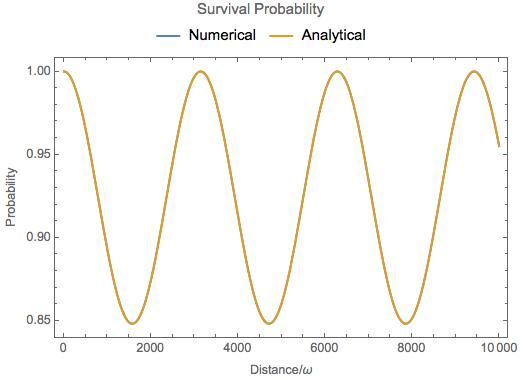
\includegraphics{vacuumOsc.jpg}
\caption{Theoretical and numerical results overlap on all the range completely.}\end{figure}


\section{3 Flavor Oscillations}
\label{vacuum:flavor-oscillations}
The vacuum Hamiltonian in mass eigenstate basis is
\begin{gather}
\begin{split}\frac{1}{2E}\begin{pmatrix}
m_1^2 & 0 & 0 \\
0 & m_2^2 &  0\\
0 & 0 & m_3^2
\end{pmatrix}.\end{split}\notag
\end{gather}
The trick to reduce the parameters is to subtract the \(\frac{m_1^2}{2E} \mathbf{I}\) from Hamiltonian in mass eigenbasis.
\begin{gather}
\begin{split}&\mathbf{H}- \frac{m_1^2}{2E}\mathbf{I} \\
=& \frac{1}{2E}\begin{pmatrix}
m_1^2 & 0 & 0 \\
0 & m_2^2 &  0\\
0 & 0 & m_3^2
\end{pmatrix} - \frac{m_1^2}{2E} \mathbf{I} \\
=& \frac{1}{2E} \begin{pmatrix}
0 & 0 & 0 \\
0 & \Delta m_{12}^2 & 0 \\
0 & 0 & \Delta m_{13}^2
\end{pmatrix},\end{split}\notag
\end{gather}
where
\begin{gather}
\begin{split}\Delta m_{12}^2 &= m_2^2 - m_1^2, \\
\Delta m_{13}^2 &= m_3^2 - m_1^2, \\
\Delta m_{23}^2 & = m_3^2 - m_2^2.\end{split}\notag
\end{gather}
Then we define the vacuum Hamiltonian in mass eigenstate basis as
\begin{gather}
\begin{split}\mathbf{H_{vm}} = \frac{1}{2E} \begin{pmatrix}
0 & 0 & 0 \\
0 & \Delta m_{12}^2 & 0 \\
0 & 0 & \Delta m_{13}^2
\end{pmatrix}\end{split}\notag
\end{gather}
To find out the representation of Hamiltonian in flavor basis, we need the PMNS matrix which transforms the mass eigenstates to flavor eigenstates,
\begin{gather}
\begin{split}\ket{\nu_\alpha}= \mathbf{U}\ket{\nu_i}.\end{split}\notag
\end{gather}
In general the matrix is
\begin{gather}
\begin{split}\mathbf U = \begin{pmatrix}
U_{11} & U_{12} & U_{13} \\
U_{21} & U_{22} & U_{23} \\
U_{31} & U_{32} & U_{33}
\end{pmatrix},\end{split}\notag
\end{gather}
with a constraint that it is unitary. To see the function of this matrix, we could use another set of indices,
\begin{gather}
\begin{split}\mathbf{U} = \begin{pmatrix}
U_{e1} & U_{e2} & U_{e3} \\
U_{\mu 1} & U_{\mu 2} & U_{\mu 3}\\
U_{\tau 1} & U_{\tau 2} & U_{\tau 3}
\end{pmatrix}.\end{split}\notag
\end{gather}
This PMNS matrix is written as
\begin{gather}
\begin{split}\mathbf{U} = \left(
\begin{array}{ccc}
 \cos \left(\theta _{12}\right) \cos \left(\theta _{13}\right) & \cos \left(\theta _{13}\right) \sin \left(\theta _{12}\right) & e^{-i \delta _{\text{CP}}} \sin \left(\theta _{13}\right) \\
 -\cos \left(\theta _{23}\right) \sin \left(\theta _{12}\right)-e^{i \delta _{\text{CP}}} \cos \left(\theta _{12}\right) \sin \left(\theta _{13}\right) \sin \left(\theta _{23}\right) & \cos \left(\theta _{12}\right) \cos \left(\theta _{23}\right)-e^{i \delta _{\text{CP}}} \sin \left(\theta _{12}\right) \sin \left(\theta _{13}\right) \sin \left(\theta _{23}\right) & \cos \left(\theta _{13}\right) \sin \left(\theta _{23}\right) \\
 \sin \left(\theta _{12}\right) \sin \left(\theta _{23}\right)-e^{i \delta _{\text{CP}}} \cos \left(\theta _{12}\right) \cos \left(\theta _{23}\right) \sin \left(\theta _{13}\right) & -e^{i \delta _{\text{CP}}} \cos \left(\theta _{23}\right) \sin \left(\theta _{12}\right) \sin \left(\theta _{13}\right)-\cos \left(\theta _{12}\right) \sin \left(\theta _{23}\right) & \cos \left(\theta _{13}\right) \cos \left(\theta _{23}\right) \\
\end{array}
\right).\end{split}\notag
\end{gather}
which is a rotation for 3D with a CP violation phase \(\delta\). For simplicity, we first assume tis phase is 0. Then the matrix becomes,
\begin{gather}
\begin{split}\mathbf{U} = \left(
\begin{array}{ccc}
 \cos \left(\theta _{12}\right) \cos \left(\theta _{13}\right) & \cos \left(\theta _{13}\right) \sin \left(\theta _{12}\right) & \sin \left(\theta _{13}\right) \\
 -\cos \left(\theta _{23}\right) \sin \left(\theta _{12}\right)-\cos \left(\theta _{12}\right) \sin \left(\theta _{13}\right) \sin \left(\theta _{23}\right) & \cos \left(\theta _{12}\right) \cos \left(\theta _{23}\right)-\sin \left(\theta _{12}\right) \sin \left(\theta _{13}\right) \sin \left(\theta _{23}\right) & \cos \left(\theta _{13}\right) \sin \left(\theta _{23}\right) \\
 \sin \left(\theta _{12}\right) \sin \left(\theta _{23}\right)-\cos \left(\theta _{12}\right) \cos \left(\theta _{23}\right) \sin \left(\theta _{13}\right) & -\cos \left(\theta _{23}\right) \sin \left(\theta _{12}\right) \sin \left(\theta _{13}\right)-\cos \left(\theta _{12}\right) \sin \left(\theta _{23}\right) & \cos \left(\theta _{13}\right) \cos \left(\theta _{23}\right) \\
\end{array}
\right).\end{split}\notag
\end{gather}
The Hamiltonian in flavor basis is found by applying the transformation that
\begin{gather}
\begin{split}\mathbf{H} &= \mathbf{U} \mathbf{H_{vm}} \mathbf{U^{-1}}.\end{split}\notag
\end{gather}\begin{figure}[htbp]
\centering
\capstart

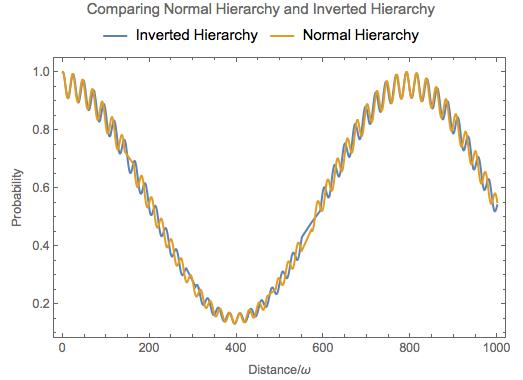
\includegraphics{vacOsc3Flavor.jpg}
\caption{Numerical results for vacuum oscillation 3 flavor case. The overall shapes are the same for NH and IH however they differ on small scales.}\end{figure}
\begin{figure}[htbp]
\centering
\capstart

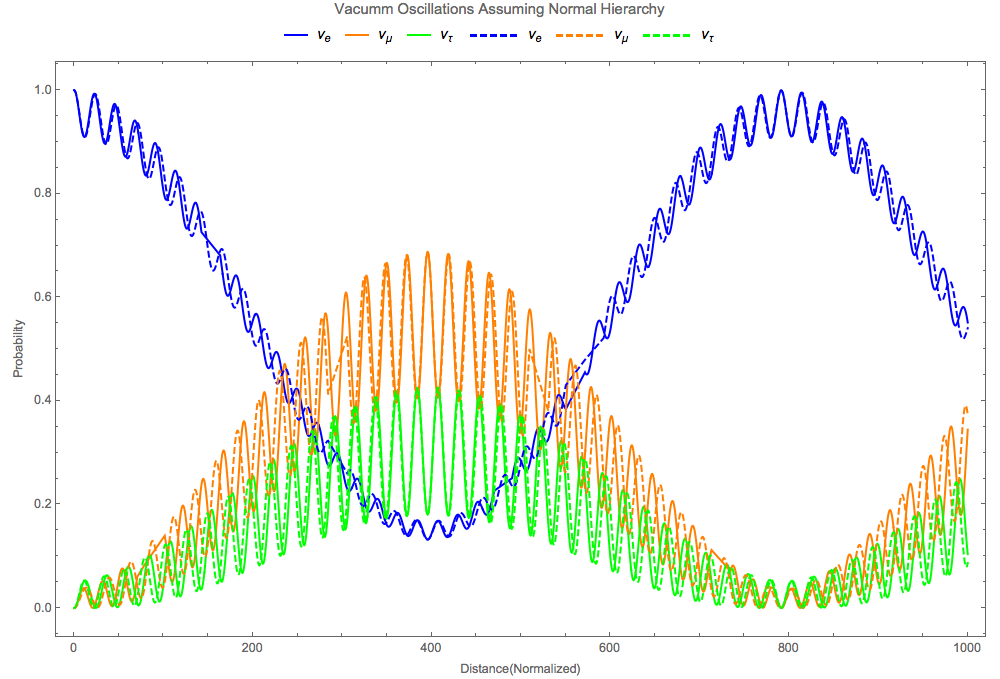
\includegraphics{vacOscNormInvComp.png}
\caption{Comparison of normal hierarchy and inverted hierarchy.The reason that they are almost the same is that the oscillation length for \(\Delta m_{13}^2\) is small thus it only changes the oscillation patterns for the small oscillations. Vacuum energy scales in normal hierarchy are}{\small \begin{gather}
\begin{split}\omega_{12} &= \frac{\Delta m_{12}^2}{2E} = 3.8\times 10^{-20}\mathrm{GeV} \\
\omega_{13} &= \frac{\Delta m_{13}^2}{2E} = 1.7\times 10^{-18}\mathrm{GeV} \\
\omega_{23} &= \frac{\Delta m_{23}^2}{2E} \approx \omega_{13}\end{split}\notag
\end{gather}
which shows that basically only two scales and the larger one determines the small oscillation.
}\end{figure}
\begin{figure}[htbp]
\centering
\capstart

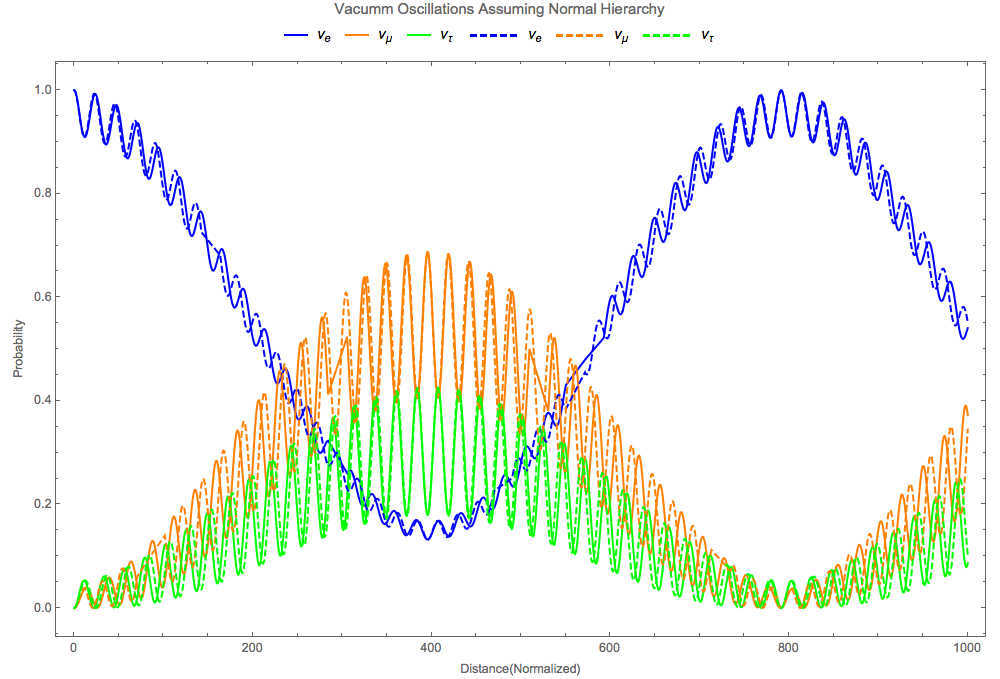
\includegraphics{vacOscNormInvComp-Invert12.png}
\caption{Comparison of normal hierarchy and inverted hierarchy but with inverted \(\Delta m_{12}^2\).}\end{figure}


\section{Ternary Diagram}
\label{vacuum:ternary-diagram}
Since the probability for differential flavors of neutrinos are summed to 1 and can be represented in barycentric coordinates, a ternary plot would be nice to understand what happens in the oscillations.
\begin{figure}[htbp]
\centering
\capstart

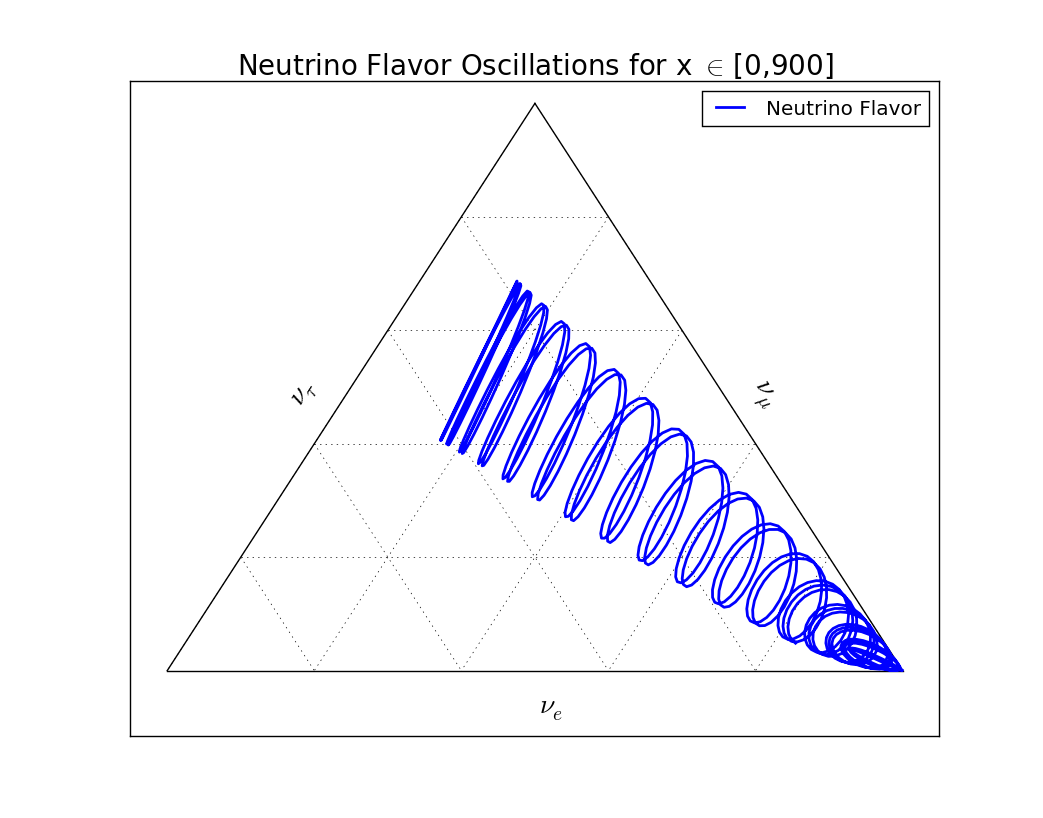
\includegraphics{vacOsc3FlavorTernary900.png}
\caption{Ternary diagram for vacuum oscillations. The state starts from bottom left, which means that the system has only electron neutrinos. As the neutrino travels, it oscillates in curves. After one period of the beat, it reaches the far end and then oscillates backwards.}\end{figure}
\begin{figure}[htbp]
\centering
\capstart

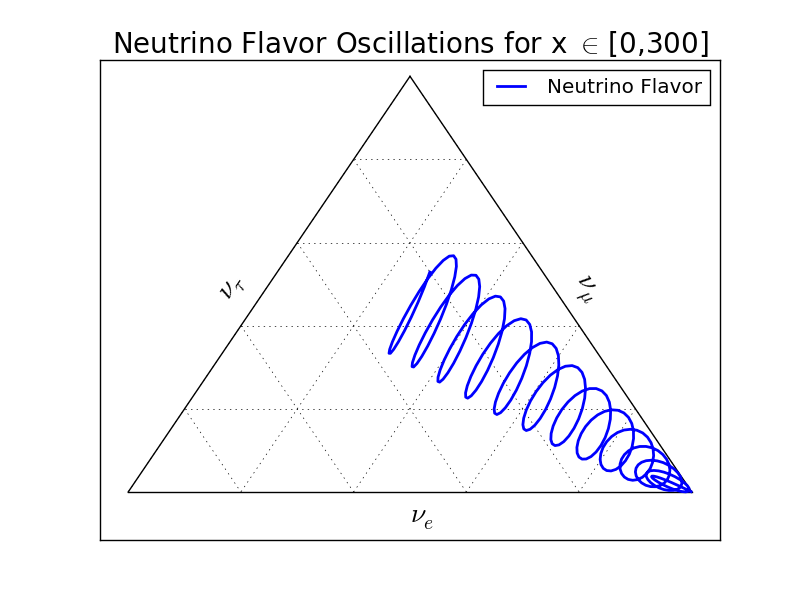
\includegraphics{vacOsc3FlavorTernary300.png}
\caption{Ternary diagram for less oscillation periods. The system starts from the right-bottom corner which is measured to be all electron neutrinos. The period of the spirals is from the energy scale that is related to a small length scale. The system spirals up then spirals back. This is a ``period'' that is governed by the energy scale that corresponds to a long length scale. Read qualitative method chapter for more about length scales.}\end{figure}
\begin{figure}[htbp]
\centering
\capstart

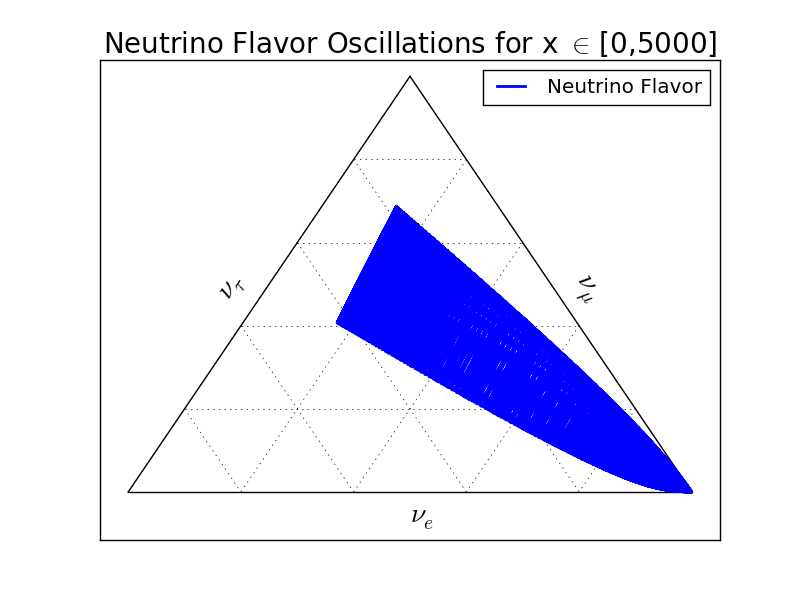
\includegraphics{vacOsc3FlavorTernary5000.png}
\caption{Ternary diagram for more oscillation periods. It shows that the system doesn't really go back to the initial state after a ``period''. This is a three body problem anyway.}\end{figure}
\begin{figure}[htbp]
\centering
\capstart

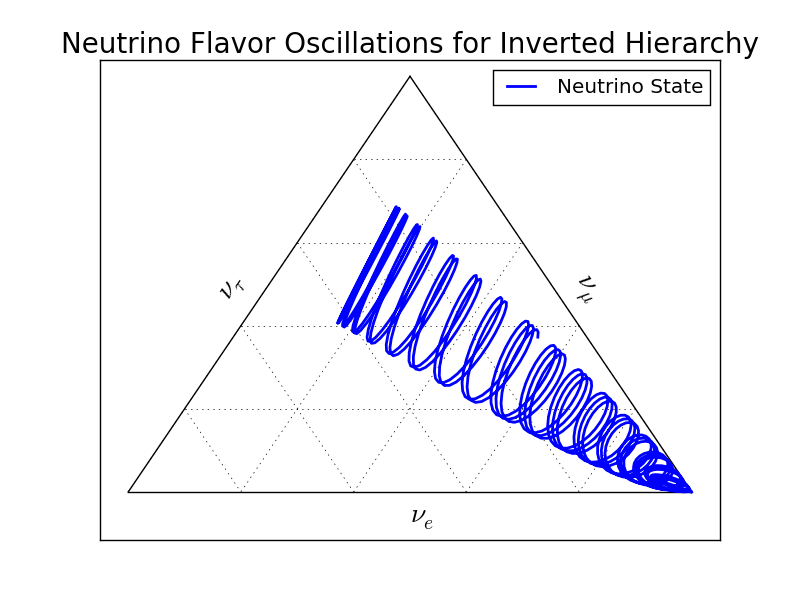
\includegraphics{Inv-1000-1.png}
\caption{Ternary diagram for inverted hierarchy. Inverted hierarchy means a period is inverted thus the spirals are in different directions.}\end{figure}


\section{Understanding the Mixing Angles}
\label{vacuum:understanding-the-mixing-angles}
The mixing angles play important roles in the amplitude of the oscillations while the energy scales play a role in the periods.
\begin{figure}[htbp]
\centering
\capstart

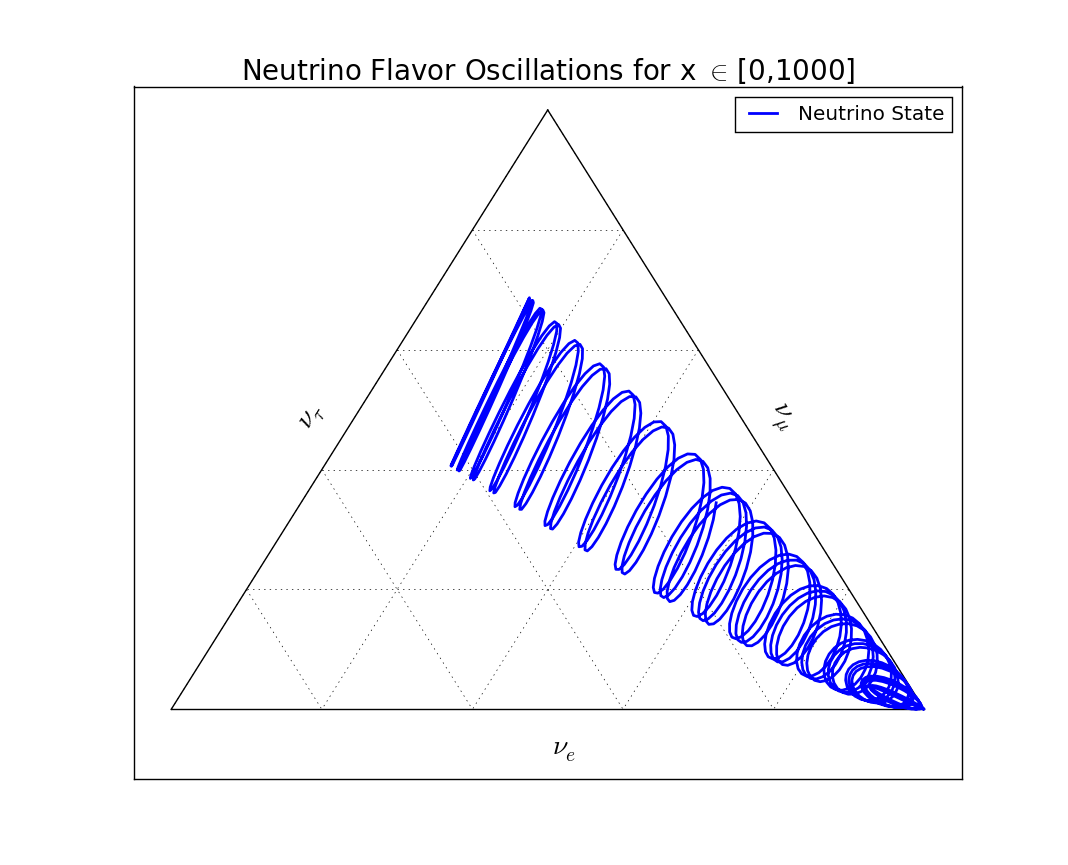
\includegraphics{1000-1.png}
\caption{Neutrino oscillations with the following parameters. This plot works as the base plot which will be compared with. The energy is scaled by a factor so that \(\frac{1}{4E}=100\mathrm{eV}\). (This scaling has no physical significance but rescales the period.)}{\small \begin{gather}
\begin{split}\theta_{12} &= 33.36/180*Pi; \\
\theta_{13} &= 8.66/180*Pi; \\
\theta_{23} &= 40/180*Pi;\\
\delta_{CP} &= 0;\\
m_1^2 &= 0.01;\\
m_2^2 &= m1sq + 0.000079.\end{split}\notag
\end{gather}}\end{figure}
\begin{figure}[htbp]
\centering
\capstart

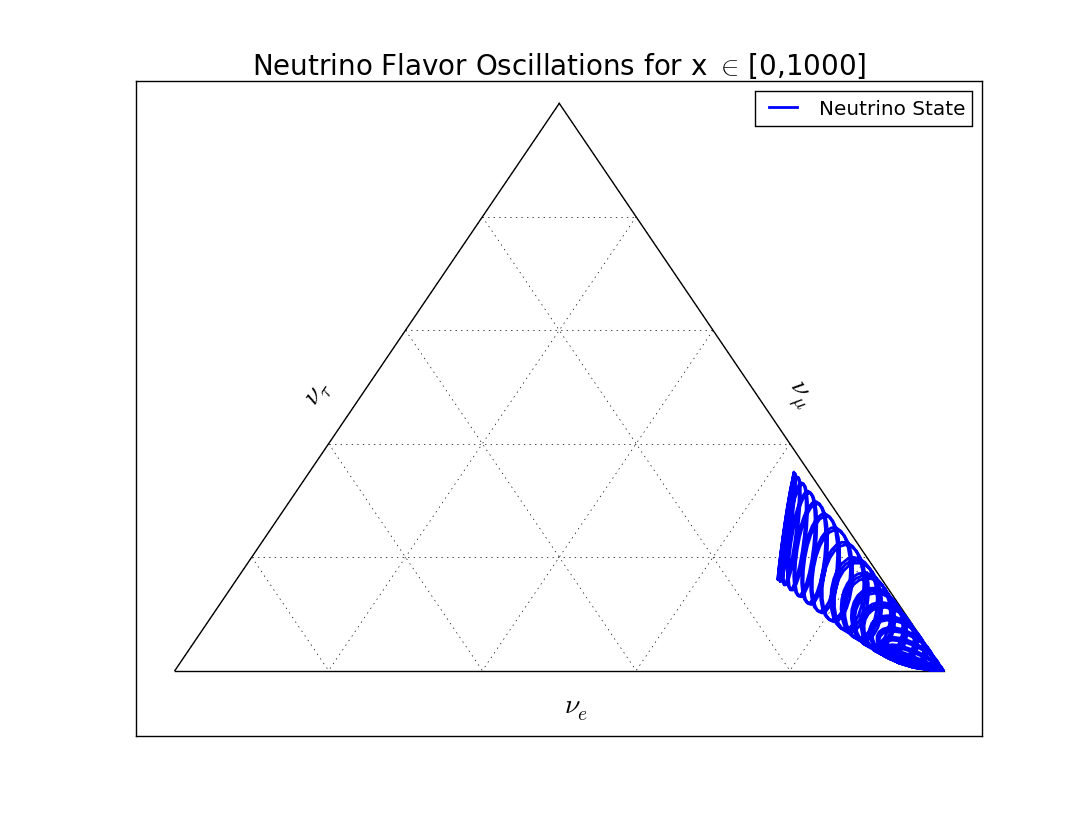
\includegraphics{1000-2.png}
\caption{Neutrino oscillations with \(\theta_{12}\) reduced to half of the value in the base plot. It is clear that \(\theta_{12}\) plays an imprtatn role in the long period of the oscillatioin. It also obvious that reducing \(\theta_{12}\) tilts the system to less \(\nu_\tau\) state.}{\small \begin{gather}
\begin{split}\theta_{12} &= 33.36/2* 180 * Pi; \\
\theta_{13} &= 8.66/180*Pi; \\
\theta_{23} &= 40/180*Pi;\\
\delta_{CP} &= 0;\\
m_1^2 &= 0.01;\\
m_2^2 &= m1sq + 0.000079.\end{split}\notag
\end{gather}}\end{figure}
\begin{figure}[htbp]
\centering
\capstart

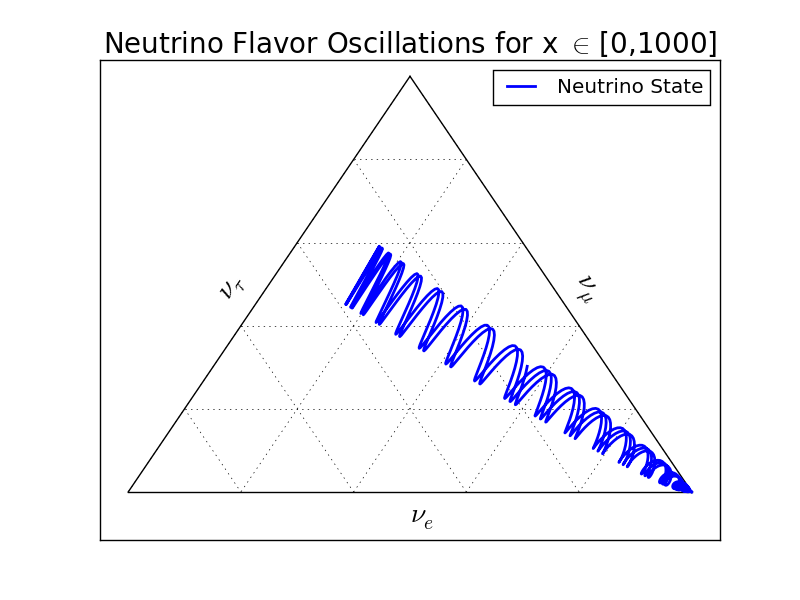
\includegraphics{1000-3.png}
\caption{Neutrino oscillations with \(\theta_{13}\) reduced to half of the value in the base plot. Reducing \(\theta_{13}\) shrinks the oscillation amplitude of the rapid oscillation.}{\small \begin{gather}
\begin{split}\theta_{12} &= 33.36/180*Pi; \\
\theta_{13} &= 8.66/ 2* 180 *Pi; \\
\theta_{23} &= 40/180*Pi;\\
\delta_{CP} &= 0;\\
m_1^2 &= 0.01;\\
m_2^2 &= m1sq + 0.000079.\end{split}\notag
\end{gather}}\end{figure}
\begin{figure}[htbp]
\centering
\capstart

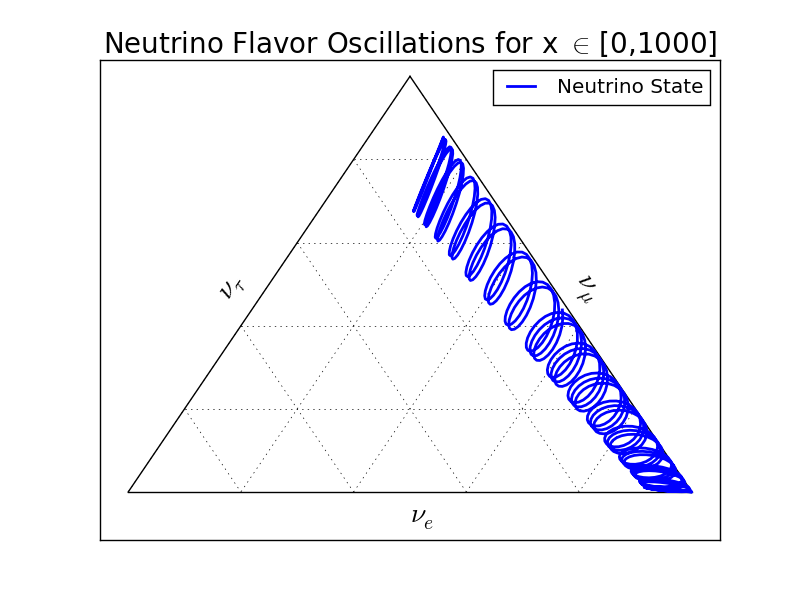
\includegraphics{1000-4.png}
\caption{Neutrino oscillations with \(\theta_{23}\) reduced to half of the value in the base plot. Reducing \(\theta_{23}\) has a complicated effect on the oscillations. But it definitely tilts the system to less \(\nu_\tau\) state. The suppression on the probability of \(\nu_\tau\) is dramatic.}{\small \begin{gather}
\begin{split}\theta_{12} &= 33.36/180*Pi; \\
\theta_{13} &= 8.66/ 180 *Pi; \\
\theta_{23} &= 40/ 2* 180*Pi;\\
\delta_{CP} &= 0;\\
m_1^2 &= 0.01;\\
m_2^2 &= m1sq + 0.000079.\end{split}\notag
\end{gather}}\end{figure}
\begin{figure}[htbp]
\centering
\capstart

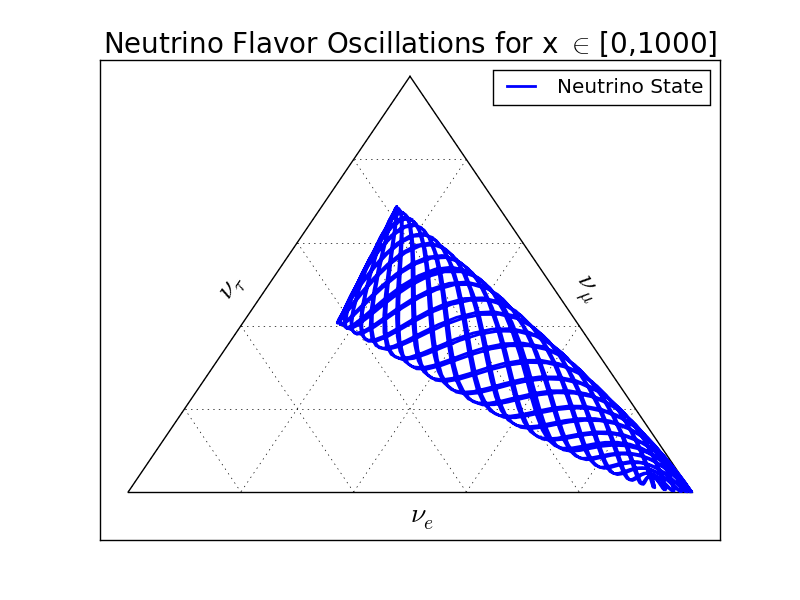
\includegraphics{1000-5.png}
\caption{Neutrino oscillations with \(\Delta m_{12}^2 = m_2^2- m_1^2\) increased compared to the value in base plot. This changes the period of the rapid oscillation.}{\small \begin{gather}
\begin{split}\theta_{12} &= 33.36/180*Pi; \\
\theta_{13} &= 8.66/180 *Pi; \\
\theta_{23} &= 40/180*Pi;\\
\delta_{CP} &= 0;\\
m_1^2 &= 0.01;\\
m_2^2 &= m1sq + 0.000079\times 10.\end{split}\notag
\end{gather}}\end{figure}
\begin{figure}[htbp]
\centering
\capstart

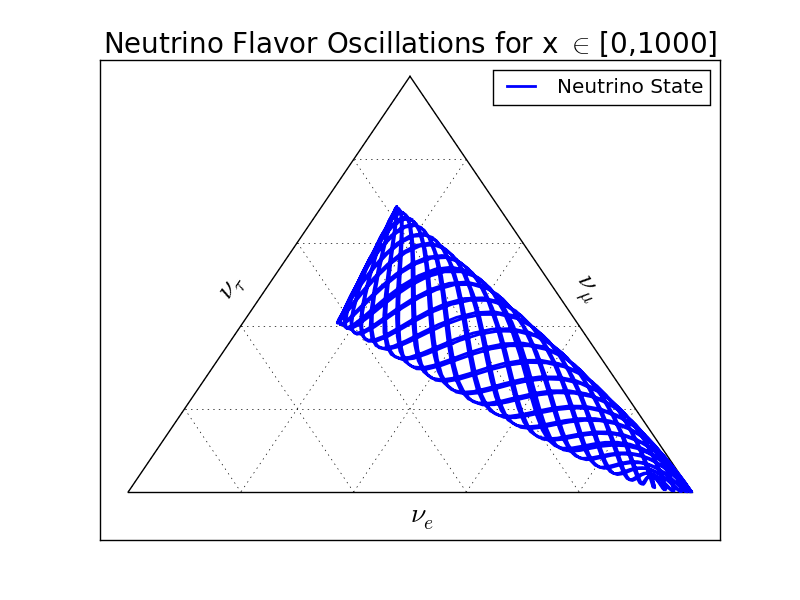
\includegraphics{1000-5.png}
\caption{Neutrino oscillation starts with initial state \(\Psi(x=0) = \nu_\mu\). The system starts from the top corner.}{\small \begin{gather}
\begin{split}\theta_{12} &= 33.36/180*Pi; \\
\theta_{13} &= 8.66/180 *Pi; \\
\theta_{23} &= 40/180*Pi;\\
\delta_{CP} &= 0;\\
m_1^2 &= 0.01;\\
m_2^2 &= m1sq + 0.000079.\end{split}\notag
\end{gather}}\end{figure}


\section{Refs and Notes}
\label{vacuum:refs-and-notes}

\chapter{Basis}
\label{basis::doc}\label{basis:basis}
Calculating neutrino oscillations requires a lot of rotations between different bases.


\section{Rotation of States}
\label{basis:rotation-of-states}
There are three most used bases, vacuum basis which diagonalizes the vacuum Hamiltonian, flavor basis where the flavor states stay, and instataneous matter basis which diagonializes the Hamiltonian with constant matter interaction or the instataneous matter interaction.
\begin{itemize}
\item {} 
The rotation from vacuum basis wavefunction \(\Psi_v\) to flavor basis \(\Psi_f\) is
\begin{gather}
\begin{split}\Psi_f = R_{v2f}(\theta_v) \Psi_v,\end{split}\notag
\end{gather}
where the rotation is
\begin{gather}
\begin{split}R_{v2f}(\theta_v) = \begin{pmatrix} \cos\theta_v & \sin \theta_v \\ -\sin \theta_v & \cos \theta_v \end{pmatrix}.\end{split}\notag
\end{gather}
\item {} 
The rotation from matter basis wavefunction \(\Psi_m\) to flavor basis wavefunction \(\Psi_f\) is
\begin{gather}
\begin{split}\Psi_f = R_{m2f}(\theta_m) \Psi_m,\end{split}\notag
\end{gather}
where the roation is
\begin{gather}
\begin{split}R_{m2f}(\theta_m) = \begin{pmatrix} \cos\theta_m & \sin \theta_m \\ -\sin \theta_m & \cos \theta_m \end{pmatrix}.\end{split}\notag
\end{gather}
The matter mixing angle is determined by the matter potential \(\lambda = \sqrt{2}G_F n_e\),
\begin{gather}
\begin{split}\tan\theta_m = \frac{\sin 2\theta_v}{\cos 2\theta_v - \lambda/\omega},\end{split}\notag
\end{gather}
where \(\omega = \delta m^2 /2E\) is the vacuum frequency of neutrinos.

\end{itemize}

\begin{notice}{note}{Rotate Twice}

A rotation from vacuum basis to flavor basis then to matter basis is simply the addition of the two rotation, i.e.,
\begin{gather}
\begin{split}R_{v2f2m}(\theta_v,\theta_m) = \begin{pmatrix} \cos(\theta_v - \theta_m) & \sin ( \theta_v - \theta_m ) \\ -\sin (\theta_v-\theta_m) & \cos (\theta_v - \theta_m) \end{pmatrix}.\end{split}\notag
\end{gather}\end{notice}


\section{Rotation of Pauli Matrices}
\label{basis:rotation-of-pauli-matrices}
Rotate \(\sigma_1\) from vacuum basis to flavor basis,
\begin{gather}
\begin{split}&R_{v2f}(\theta) \sigma_1 R_{v2f}^{\dagger} \\
=& \sin 2\theta \sigma_3 + \cos 2\theta \sigma_1.\end{split}\notag
\end{gather}
Rotate \(\sigma_3\) from vacuum basis to flavor basis,
\begin{gather}
\begin{split}&R_{v2f}(\theta) \sigma_3 R_{v2f}^{\dagger} \\
=&  \begin{pmatrix} \cos \theta & \sin \theta \\ -\sin \theta & \cos\theta \end{pmatrix} \begin{pmatrix} 1 & 0 \\ 0 & -1 \end{pmatrix} \begin{pmatrix} \cos \theta & -\sin \theta \\ \sin \theta & \cos\theta \end{pmatrix} \\
=& \cos 2\theta \sigma_3 - \sin 2\theta \sigma_1.\end{split}\notag
\end{gather}

\section{Rotation of Hamiltonian}
\label{basis:rotation-of-hamiltonian}
Given the vacuum basis Hamiltonian \(H_v\), we can rotation it to flavor basis by using the rotation \(R_{v2f}(\theta_v)\)
\begin{gather}
\begin{split}H_f = R_{v2f}(\theta_v) H_v R_{v2f}^{-1}(\theta_v).\end{split}\notag
\end{gather}
Similarly, the flavor basis Hamiltonian \(H_f\) can also be calculated from matter basis Hamiltonian \(H_m\) ,
\begin{gather}
\begin{split}H_f = R_{m2f}(\theta_m) H_m R_{v2f}^{-1}(\theta_m).\end{split}\notag
\end{gather}
\begin{notice}{note}{Vacuum Basis Hamiltonian}

The Hamiltonian in this basis is composed of vacuum Hamiltonian which is diagonalized and the matter potential rotated from flavor basis,
\begin{gather}
\begin{split}H_v &= -\frac{\omega}{2} \sigma_3 + \frac{\lambda}{2} \begin{pmatrix} \cos \theta & -\sin \theta \\ \sin \theta & \cos\theta \end{pmatrix}  \sigma_3 \begin{pmatrix} \cos \theta & \sin \theta \\ -\sin \theta & \cos\theta \end{pmatrix} \\
&= -\frac{\omega}{2} \sigma_3 + \frac{\lambda}{2}\cos 2\theta_v \sigma_3 + \frac{\lambda}{2} \sin 2\theta_v \sigma_1.\end{split}\notag
\end{gather}\end{notice}

\begin{notice}{note}{Flavor Basis Hamiltonian}
\begin{gather}
\begin{split}H_f = - \frac{\omega}{2} \cos 2\theta \sigma_3 +  \frac{\omega}{2} \sin 2\theta \sigma_1 +  \frac{\lambda}{2} \sigma_3.\end{split}\notag
\end{gather}\end{notice}

As a consistancy check, we now rotate Hamiltonian in vacuum basis to flavor basis.
\begin{gather}
\begin{split}H_f &= \begin{pmatrix} \cos \theta & \sin \theta \\ -\sin \theta & \cos\theta \end{pmatrix} H_v \begin{pmatrix} \cos \theta & -\sin \theta \\ \sin \theta & \cos\theta \end{pmatrix}\\
&= \left(-\frac{\omega}{2} + \frac{\lambda}{2} \cos 2\theta \right) \begin{pmatrix} \cos \theta & \sin \theta \\ -\sin \theta & \cos\theta \end{pmatrix} \sigma_3 \begin{pmatrix} \cos \theta & -\sin \theta \\ \sin \theta & \cos\theta \end{pmatrix} + \frac{\lambda}{2} \sin 2\theta \begin{pmatrix} \cos \theta & \sin \theta \\ -\sin \theta & \cos\theta \end{pmatrix} \sigma_1 \begin{pmatrix} \cos \theta & -\sin \theta \\ \sin \theta & \cos\theta \end{pmatrix} \\
& = \left(-\frac{\omega}{2} + \frac{\lambda}{2} \cos 2\theta \right) ( \cos 2\theta \sigma_3 - \sin 2\theta \sigma_1 ) + \frac{\lambda}{2}\sin 2\theta ( \sin 2\theta \sigma_3 + \cos 2\theta \sigma_1 ) \\
& = -\frac{\omega}{2} \cos 2\theta \sigma_3 + \frac{\omega}{2}\sin 2\theta \sigma_1 + \frac{\lambda}{2} ( \cos^2 2\theta + \sin ^2 2\theta ) \sigma_3 \\
& = -\frac{\omega}{2} \cos 2\theta \sigma_3 + \frac{\omega}{2}\sin 2\theta \sigma_1 + \frac{\lambda}{2}\sigma_3 .\end{split}\notag
\end{gather}
\begin{notice}{note}{Numerical Calculation of The Rotations}

To write clean code, it is better to define and test there rotations first.
\end{notice}


\section{Rotating Basis}
\label{basis:rotating-basis}
In vacuum basis, Hamiltonian is
\begin{gather}
\begin{split}H_v = -\frac{\omega}{2} \sigma_3 + \frac{\lambda}{2}\cos 2\theta_v \sigma_3 + \frac{\lambda}{2} \sin 2\theta_v \sigma_1,\end{split}\notag
\end{gather}
where we have got a contribution of \(\sigma_3\) from matter interaction. By carefully defining a transformation that removes this contribution, we can define a new basis in which the wavefunction is \(\Psi_b\), which is related to the vacuum basis wavefunction in the following way,
\begin{gather}
\begin{split}\begin{pmatrix}\psi_{v1} \\ \psi_{v2} \end{pmatrix}  = \begin{pmatrix}
e^{-i \eta(x) x} & 0 \\  0 & e^{i \eta(x) x}
\end{pmatrix} \begin{pmatrix}\psi_{b1} \\ \psi_{b2} \end{pmatrix},\end{split}\notag
\end{gather}
where \(\eta(x)\) is a function of position. We can find the requirement of it by plug the wavefunction into Schrodinger equation, which results in
\begin{gather}
\begin{split}\eta + x \frac{d\eta }{dx} = \frac{\lambda}{2} \cos 2\theta_v.\end{split}\notag
\end{gather}
The general solution is
\begin{gather}
\begin{split}\eta(x) = \frac{Constant}{x} + \frac{1}{x} \int_1^x \frac{\cos 2\theta_v}{2} \lambda(\tau) d\tau,\end{split}\notag
\end{gather}
where the constant can always be set to 0, which tells us that
\begin{gather}
\begin{split}\eta(x) = \frac{1}{x} \int_1^x \frac{\cos 2\theta_v}{2} \lambda(\tau) d\tau .\end{split}\notag
\end{gather}
\begin{notice}{note}{Constant Matter Density}

As a check, for constant \(\lambda\), we have
\begin{gather}
\begin{split}\eta(x) = \frac{\cos 2\theta_v }{2x} \lambda ( x-1 ).\end{split}\notag
\end{gather}\end{notice}

In this new basis, the Hamiltonian becomes
\begin{gather}
\begin{split}H_b &= - \frac{\omega}{2} \sigma_3 + \frac{\lambda}{2} \sin 2\theta_v \begin{pmatrix} 0 & e^{i 2\eta(x) x} \\ e^{ - i 2\eta(x) x} & 0  \end{pmatrix} \\
& =  - \frac{\omega}{2} \sigma_3 + \frac{\lambda}{2}\sin 2\theta_v \cos ( 2\eta(x) x )\sigma_1 - \frac{\lambda}{2} \sin 2\theta_v \sin (2\eta(x) x) \sigma_2.\end{split}\notag
\end{gather}

\section{Refs \& Notes}
\label{basis:refs-notes}

\chapter{Interaction With Matter}
\label{msw:interaction-with-matter}\label{msw::doc}
\index{MSW effect}

\section{MSW Effect}
\label{msw:index-0}\label{msw:msw-effect}
\begin{notice}{note}{Physics of MSW}

As neutrinos passing by matter, the effective mass coming from energy change becomes important thus changing it's eigenstates and propagation.
\end{notice}

Neutrinos do interact with matter, mostly electrons in most cases.
\begin{figure}[htbp]
\centering

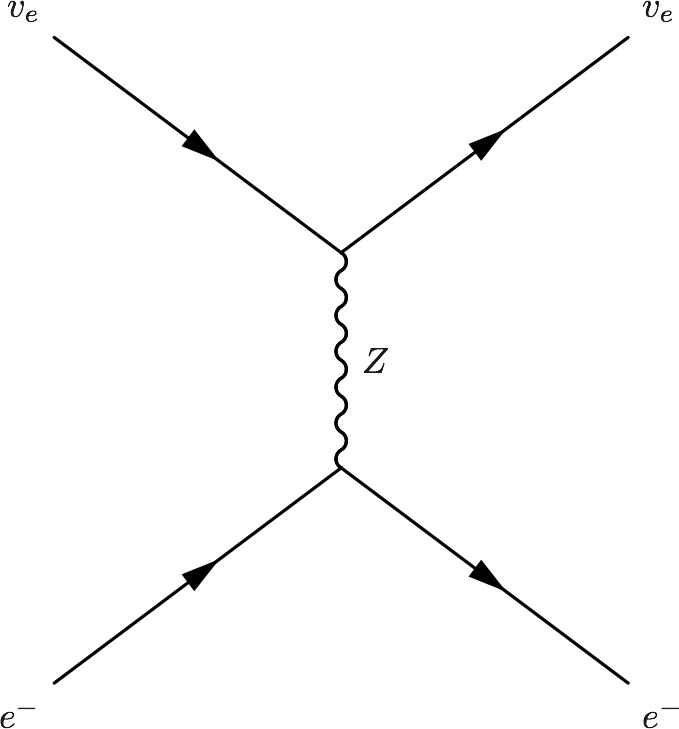
\includegraphics{nueNeutral.png}
\end{figure}

\begin{Verbatim}[commandchars=\\\{\}]
\PYGZbs{}begin\PYGZob{}fmfgraph*\PYGZcb{}(200,180)
  \PYGZbs{}fmfleft\PYGZob{}i1,i2\PYGZcb{}
  \PYGZbs{}fmfright\PYGZob{}o1,o2\PYGZcb{}
  \PYGZbs{}fmf\PYGZob{}fermion\PYGZcb{}\PYGZob{}i1,v1,o1\PYGZcb{}
  \PYGZbs{}fmf\PYGZob{}fermion\PYGZcb{}\PYGZob{}i2,v2,o2\PYGZcb{}
  \PYGZbs{}fmf\PYGZob{}photon\PYGZcb{}\PYGZob{}v1,v2\PYGZcb{}
  \PYGZbs{}fmflabel\PYGZob{}\PYGZdl{}v\PYGZus{}e\PYGZdl{}\PYGZcb{}\PYGZob{}i2\PYGZcb{}
  \PYGZbs{}fmflabel\PYGZob{}\PYGZdl{}e\PYGZca{}\PYGZhy{}\PYGZdl{}\PYGZcb{}\PYGZob{}i1\PYGZcb{}
  \PYGZbs{}fmflabel\PYGZob{}\PYGZdl{}v\PYGZus{}e\PYGZdl{}\PYGZcb{}\PYGZob{}o2\PYGZcb{}
  \PYGZbs{}fmflabel\PYGZob{}\PYGZdl{}e\PYGZca{}\PYGZhy{}\PYGZdl{}\PYGZcb{}\PYGZob{}o1\PYGZcb{}
  \PYGZbs{}fmf\PYGZob{}photon,label=\PYGZdl{}Z\PYGZdl{}\PYGZcb{}\PYGZob{}v1,v2\PYGZcb{}
\PYGZbs{}end\PYGZob{}fmfgraph*\PYGZcb{}
\end{Verbatim}
\begin{figure}[htbp]
\centering

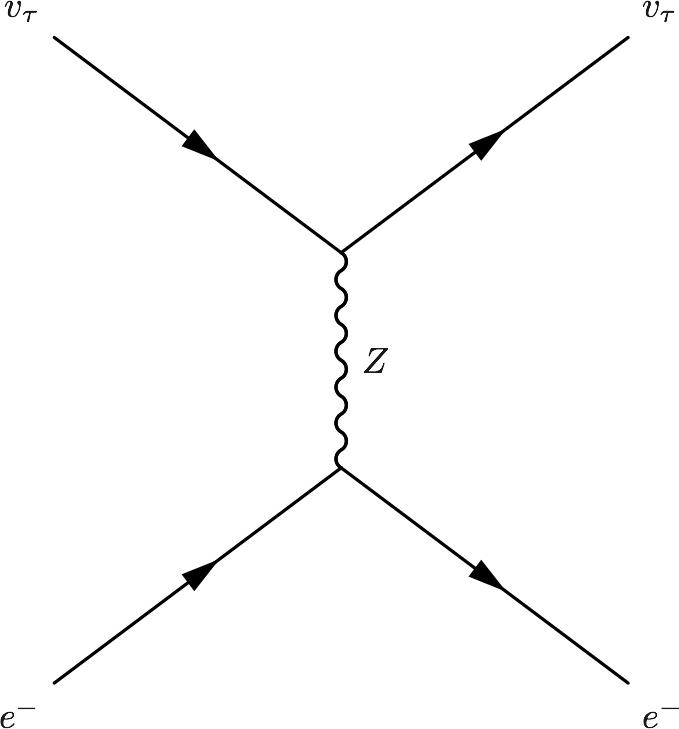
\includegraphics{nutaueNeutral.png}
\end{figure}

\begin{Verbatim}[commandchars=\\\{\}]
\PYGZbs{}begin\PYGZob{}fmfgraph*\PYGZcb{}(200,180)
 \PYGZbs{}fmfleft\PYGZob{}i1,i2\PYGZcb{}
 \PYGZbs{}fmfright\PYGZob{}o1,o2\PYGZcb{}
 \PYGZbs{}fmf\PYGZob{}fermion\PYGZcb{}\PYGZob{}i1,v1,o1\PYGZcb{}
 \PYGZbs{}fmf\PYGZob{}fermion\PYGZcb{}\PYGZob{}i2,v2,o2\PYGZcb{}
 \PYGZbs{}fmf\PYGZob{}photon\PYGZcb{}\PYGZob{}v1,v2\PYGZcb{}
 \PYGZbs{}fmflabel\PYGZob{}\PYGZdl{}v\PYGZus{}\PYGZbs{}tau\PYGZdl{}\PYGZcb{}\PYGZob{}i2\PYGZcb{}
 \PYGZbs{}fmflabel\PYGZob{}\PYGZdl{}e\PYGZca{}\PYGZhy{}\PYGZdl{}\PYGZcb{}\PYGZob{}i1\PYGZcb{}
 \PYGZbs{}fmflabel\PYGZob{}\PYGZdl{}v\PYGZus{}\PYGZbs{}tau\PYGZdl{}\PYGZcb{}\PYGZob{}o2\PYGZcb{}
 \PYGZbs{}fmflabel\PYGZob{}\PYGZdl{}e\PYGZca{}\PYGZhy{}\PYGZdl{}\PYGZcb{}\PYGZob{}o1\PYGZcb{}
 \PYGZbs{}fmf\PYGZob{}photon,label=\PYGZdl{}Z\PYGZdl{}\PYGZcb{}\PYGZob{}v1,v2\PYGZcb{}
\PYGZbs{}end\PYGZob{}fmfgraph*\PYGZcb{}
\end{Verbatim}
\begin{figure}[htbp]
\centering

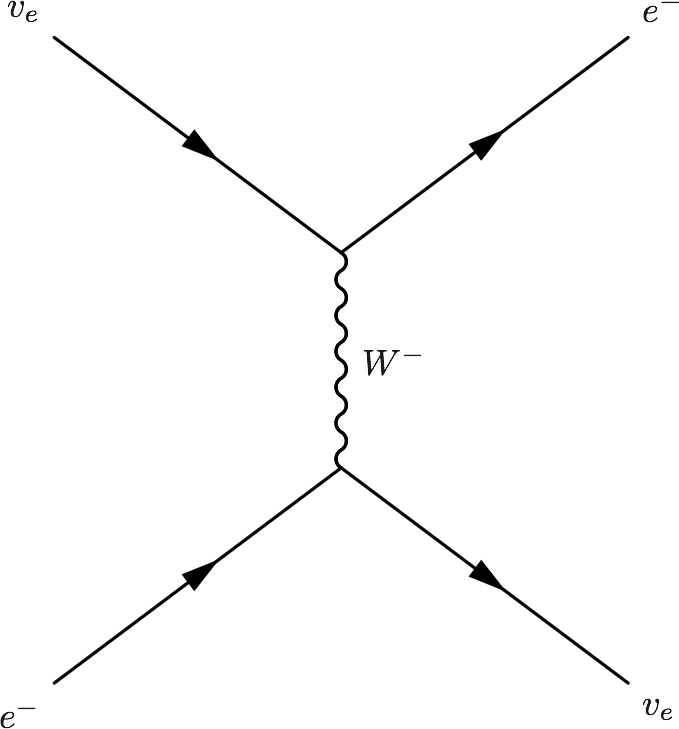
\includegraphics{nueCharged.png}
\end{figure}

\begin{Verbatim}[commandchars=\\\{\}]
\PYGZbs{}begin\PYGZob{}fmfgraph*\PYGZcb{}(200,180)
 \PYGZbs{}fmfleft\PYGZob{}i1,i2\PYGZcb{}
 \PYGZbs{}fmfright\PYGZob{}o1,o2\PYGZcb{}
 \PYGZbs{}fmf\PYGZob{}fermion\PYGZcb{}\PYGZob{}i1,v1,o1\PYGZcb{}
 \PYGZbs{}fmf\PYGZob{}fermion\PYGZcb{}\PYGZob{}i2,v2,o2\PYGZcb{}
 \PYGZbs{}fmf\PYGZob{}photon\PYGZcb{}\PYGZob{}v1,v2\PYGZcb{}
 \PYGZbs{}fmflabel\PYGZob{}\PYGZdl{}v\PYGZus{}e\PYGZdl{}\PYGZcb{}\PYGZob{}i2\PYGZcb{}
 \PYGZbs{}fmflabel\PYGZob{}\PYGZdl{}e\PYGZca{}\PYGZhy{}\PYGZdl{}\PYGZcb{}\PYGZob{}i1\PYGZcb{}
 \PYGZbs{}fmflabel\PYGZob{}\PYGZdl{}v\PYGZus{}e\PYGZdl{}\PYGZcb{}\PYGZob{}o1\PYGZcb{}
 \PYGZbs{}fmflabel\PYGZob{}\PYGZdl{}e\PYGZca{}\PYGZhy{}\PYGZdl{}\PYGZcb{}\PYGZob{}o2\PYGZcb{}
 \PYGZbs{}fmf\PYGZob{}photon,label=\PYGZdl{}W\PYGZca{}\PYGZob{}\PYGZhy{}\PYGZcb{}\PYGZdl{}\PYGZcb{}\PYGZob{}v1,v2\PYGZcb{}
\PYGZbs{}end\PYGZob{}fmfgraph*\PYGZcb{}
\end{Verbatim}

The one that is missing is the charged current for \(nu_\tau\) and \(e^{-}\) interaction because of lepton number conservation.

The first two diagrams will add two equal terms on the diagonal terms of Hamiltonian, which can be viewed as adding a number times identity matrix thus conserves the eigenstates while shifts the eigenvalues. However, the third diagram will only add a term to the first diagonal term of Hamiltonian, which is the weak coupling \(\Delta = \sqrt{2}G_F n(x)\) with \(n(x)\) being the number density of electrons.

\begin{notice}{note}{Identity Matrix and Survival Probability}

Identity matrix shifts the eigenvalues up and down homogeneously which changes the evolution of the state. However, since this is only a phase, the calculation of the survival probability will kill this phase.
\end{notice}

\begin{notice}{note}{Weak Interaction}

We can guess this interaction term using physics picture. This interaction should be proportional to density of electrons with a coupling constant \(G_F\). Then check the dimensions.
\begin{gather}
\begin{split}[G_F] &= [E]^{-2} \\
[n(x)] & = [E]^3\end{split}\notag
\end{gather}
So the dimension is right. The missing constant is \(\sqrt{2}\).
\end{notice}

This symmetry breaking will change the evolution and makes the states more electron neutrino.

This is the reason of MSW effect.

In other words, the first requirement of MSW effect is that the electrons interacts with neutrinos and makes it in a specific state that is heavy if the electron density is strong enough. Meanwhile, if the mixing angle is not that large, a level crossing could happen making the state a light state as the density becomes vacuum. The other requirement, which is obvious, is that the density change should be adiabatic, the meaning of which is the density profile of matter gently reduces to vacuum, leaving enough reaction time for the neutrinos.

The MSW effect itself can be made clear using the example of neutrino oscillations in our sun.

\begin{notice}{note}{Small Mixing Angle}

Take two flavour mixing as an example.
\begin{gather}
\begin{split}\begin{pmatrix}\nu_e \\ \nu_x\end{pmatrix} = \begin{pmatrix}  \cos\theta & \sin\theta \\ -\sin\theta  & \cos\theta \end{pmatrix}   \begin{pmatrix}\nu_1 \\ \nu_2\end{pmatrix}\end{split}\notag
\end{gather}
In the small mixing angle limit,
\begin{gather}
\begin{split}\begin{pmatrix}\nu_e \\ \nu_x\end{pmatrix} \to \begin{pmatrix}  1 & \theta \\ -\theta  & 1 \end{pmatrix}   \begin{pmatrix}\nu_1 \\ \nu_2\end{pmatrix}\end{split}\notag
\end{gather}
which is very close to an identity matrix. This implies that electron neutrino is more like mass eigenstate \(\nu_1\). By \(\nu_1\) we mean the state with energy \(\frac{ \Delta m^2 }{4E}\) in vacuum.

We need this intuitive picture to understand MSW effect. Electron neutrinos are almost identical to the low mass neutrino mass eigenstate. \textbf{However, as we will see, due to the matter interaction, the electron flavour neutrino is corresponding to the HEAVY mass eigenstate.} This is the key idea in physics of MSW effect.
\end{notice}

The Hamiltonian for neutinos with neutrino-matter interaction (in flavour basis) is
\begin{gather}
\begin{split}\mathbf H = \frac{ \Delta m^2 }{4E}\begin{pmatrix} -\cos 2\theta & \sin 2\theta \\ \sin 2\theta & \cos 2\theta \end{pmatrix}  {\color{red} + \frac{\Delta}{2} \mathbf {\sigma_3}}  {\color{green}+ \Delta \mathbf I},\end{split}\notag
\end{gather}
where the last term (green part) can be neglected because this term will only shift all the eigenvalues with the same amount without changing the eigenvectors.

Define a quantities like \(\omega=\frac{ \Delta m^2 }{2E}\) for neutrinos ( \(\bar\omega = \frac{ \Delta m^2 }{-2E}\) for antineutrinos) and \(\Delta = \sqrt{2} G_F n(x)\) (which might be denoted by \(\nu = \sqrt{2}G_F n_\nu\) in other lituratures).

Using Pauli matrices, I can decompose this to
\begin{gather}
\begin{split}\mathbf H = \frac{\omega}{2}( -\cos2\theta \sigma_3 + \sin 2\theta \sigma_1 )   {\color{red} + \frac{\Delta}{2} \mathbf {\sigma_3}}  {\color{green}+ \Delta \mathbf I}\end{split}\notag
\end{gather}
\begin{notice}{note}{Note:}
As a reminder, \(\Delta = \sqrt{2}G_F n(x)\).
\end{notice}

\begin{notice}{note}{Note:}
The red part is from the charged current Feynman diagram. We have a \(\mathbf\sigma_3\) matrix instead of an matrix like
\begin{gather}
\begin{split}\begin{pmatrix}1 & 0 \\ 0 & 0 \end{pmatrix}\end{split}\notag
\end{gather}
because we rewrite this matrix with Pauli matrices and identy. Then the identities are neglected.

This can be done properly because Pauli matrice and Identy matrix form a complete basis.
\end{notice}

In a more compact form, this Hamiltonian is
\begin{gather}
\begin{split}\mathbf H &= \frac{ \Delta m^2 }{4E} \left( -\cos 2\theta \mathbf {\sigma_3 } + \sin 2\theta \mathbf{\sigma_1} \right)  {\color{red} + \frac{\Delta}{2} \mathbf {\sigma_3}} \\
& = \left(\frac{\Delta}{2} -\frac{ \Delta m^2 }{4E} \cos 2\theta\right) \mathbf {\sigma_3 } + \frac{ \Delta m^2 }{4E} \sin 2\theta \mathbf{\sigma_1}\end{split}\notag
\end{gather}
\begin{notice}{note}{Note:}
Eigenvalues of \(\mathbf {\sigma_3}\) are 1 and -1 with corresponding eigenvectors
\begin{gather}
\begin{split}\begin{pmatrix}1\\ 0 \end{pmatrix}\end{split}\notag
\end{gather}
and
\begin{gather}
\begin{split}\begin{pmatrix}0\\ 1 \end{pmatrix}.\end{split}\notag
\end{gather}\end{notice}

As we have mentioned, this Hamiltonian is in flavour basis. When mixing angle \(\theta \to 0\), the eigenvectors are almost eigenvectors of \(\mathbf{\sigma_3}\) which are electron neutrinos and x type neutrinos.

\begin{notice}{note}{Interesting Limits}

Before we really solve the equation of motion, some interesting limits can be shown here.

\textbf{Interaction} \(\Delta\) \textbf{is much larger than cacuum mixing terms.} In this case, the Hamiltonian becomes diagonalized and the neutrinos will stay on it's flavour eigenstates in the propagation.

\textbf{Interaction} \(\Delta\) \textbf{is much smaller than vacuum mixing terms.} The propagation reduces to vacuum case.
\end{notice}

To see this effect quantitively, we need to diagonalize this Hamiltonian (\textbf{Can we actually diagonalize the equation of motion? NO!}). Equivalently, we can rewrite it in the basis of mass eigenstates \(\{\ket{\nu_L(x)}, \ket{\nu_H(x)}\}\),
\begin{gather}
\begin{split}\ket{\nu_L(x)} &= \cos\theta(x) \ket{\nu_e} - \sin\theta(x) \ket{\nu_\mu} \\
\ket{\nu_H(x)} & =  \sin\theta(x) \ket{\nu_e} - \cos\theta(x) \ket{\nu_\mu}.\end{split}\notag
\end{gather}
This new rotation in matrix form is
\begin{gather}
\begin{split}\begin{pmatrix} \ket{\nu_L(x)} \\ \ket{\nu_H(x)} \end{pmatrix} &= \begin{pmatrix} \cos \theta(x) & -\sin\theta(x) \\ \sin\theta(x) & \cos\theta(x) \end{pmatrix} \begin{pmatrix}\ket{\nu_e} \\ \ket{\nu_x} \end{pmatrix} \\
& = \mathbf{U^{-1}_x } \begin{pmatrix}\ket{\nu_e} \\ \ket{\nu_x} \end{pmatrix}\end{split}\notag
\end{gather}
\begin{notice}{note}{Diagonalize Hamiltonian}

To diagonilize it, we need to multiply on both sides the rotation matrix and its inverse,
\begin{gather}
\begin{split}\mathbf {H_{xd}} = \mathbf{U_x^{-1}} \mathbf H \mathbf {U_x}.\end{split}\notag
\end{gather}
The second step is to set the off diagonal elements to zero. By solving the equaions we can find the \(\sin 2\theta(x)\) and \(\cos 2\theta(x)\).
\begin{gather}
\begin{split}\mathbf{H_{xd}} &= \mathbf{U^{-1}_x} \left( A_1 \mathbf{\sigma_1} + A_3 \mathbf{\sigma_3} \right) \mathbf{ U_x } \\
& = \begin{pmatrix} A_3\cos 2\theta(x) - A_1 \sin 2\theta(x) & A_3 \sin 2\theta(x) + A_1 \cos 2\theta(x) \\ A_3 \sin 2\theta(x) + A_1\cos 2\theta(x) &  - A_3 \cos 2\theta(x) + A_1 \sin 2\theta(x) \end{pmatrix},\end{split}\notag
\end{gather}
where
\begin{gather}
\begin{split}A_3 &  = \frac{\Delta}{2} - \frac{\delta^2 m}{4E}\cos 2\theta \\
A_1 & =  \frac{\delta^2 m}{4E} \sin 2\theta.\end{split}\notag
\end{gather}
Set the off-diagonal elements to zero,
\begin{gather}
\begin{split}A_3 \sin 2\theta(x) + A_1 \cos 2\theta(x)  = 0\end{split}\notag
\end{gather}
So the solutions are
\begin{gather}
\begin{split}\sin 2\theta(x) & = \frac{A_1}{\sqrt{A_1^2 + A_3^2}} \\
\cos 2\theta(x) & = \frac{-A_3}{\sqrt{A_1^2+A_3^2}}.\end{split}\notag
\end{gather}
Plug in \(A_1\) and \(A_3\)
\begin{gather}
\begin{split}\sin 2\theta(x)  &= \frac{\sin 2\theta_v}{\sqrt{ \left(\frac{\Delta}{\omega} \right)^2+1 - 2 \frac{\Delta}{\omega}\cos 2\theta_v }} \\
\cos 2\theta(x)&= \frac{ \cos 2\theta_v - \frac{\Delta}{\omega} }{ \sqrt{ \left( \frac{\Delta}{\omega} \right)^2  +1 - 2 \frac{\Delta}{\omega}\cos 2\theta_v  }}.\end{split}\notag
\end{gather}
Define \(\hat\Delta = \frac{\Delta}{\omega}\) with \(\omega=\frac{\Delta m^2}{2E}\), which represents the matter interaction strength compared to the vacuum oscillation.
\begin{gather}
\begin{split}\sin 2\theta(x)  &= \frac{\sin 2\theta_v}{\sqrt{ \hat\Delta ^2+1 - 2 \hat\Delta \cos 2\theta_v }} \\
\cos 2\theta(x)&= \frac{ \cos 2\theta_v - \hat\Delta  }{ \sqrt{\hat\Delta ^2  +1 - 2 \hat\Delta \cos 2\theta_v } }.\end{split}\notag
\end{gather}
We also have
\begin{gather}
\begin{split}A_3\cos 2\theta(x) - A_1 \sin 2\theta(x) = -\frac{\omega}{2}\sqrt{\hat \Delta^2 +1 - 2\hat\Delta \cos 2\theta_v},\end{split}\notag
\end{gather}
which leads to the result of the diagonalized Hamiltonian
\begin{gather}
\begin{split}\mathbf{H_{xd}} = \frac{\omega}{2}\sqrt{\Delta^2 +1 - 2\hat\Delta \cos 2\theta_v} \begin{pmatrix}
-1 & 0 \\
0 & 1
\end{pmatrix}.\end{split}\notag
\end{gather}
\textbf{This diagonalize the Hamiltonian LOCALLY. It's not possible to diagonalize the Hamiltonian globally if the electron number density is not a constant.}

\textbf{The point is, for equation of motion, we have a differentiation with respect to position} \(x\)! \textbf{So even we diagonalize the Hamiltonian, the equation of motion won't be diagonalized. An extra matrix will occur on the LHS and de-diagonalize the Hamiltonian on RHS.}
\end{notice}

\begin{notice}{note}{Note:}
As \(\Delta \to \infty\), \(A_3\to \infty\) and \(\sin 2\theta(x)\) vanishes. Thus the neutrino will stay on flavour eigenstates.
\end{notice}

With the newly defined heavy-light mass eigenstates, we can calculate the propagatioin of neutrinos,
\begin{gather}
\begin{split}i \hbar \partial_t \ket{\psi_x(t)} = \mathbf{Extra Matrix From LHS}\cdot \mathbf H_{xd} \ket{\psi_x(t)},\end{split}\notag
\end{gather}
where the \(\mathbf{Extra Matrix From LHS}\) comes from the fact that changing from flavor basis \(\Psi(x)\) to heavy-light basis \(\Psi_m(x)\) using \(\mathbf {U_m}\),
\begin{gather}
\begin{split}i\partial_x (\mathbf{U_m} \Psi_m(x)) = H ( \mathbf{U_m} \Psi_m(x) )\end{split}\notag
\end{gather}
only returns
\begin{gather}
\begin{split}i\partial_x \Psi_m(x) = \mathbf{H_{md} } \Psi_m(x) - i \mathbf{U_m^{-1}} ( \partial_x \mathbf{U_m} ) \Psi_m(x).\end{split}\notag
\end{gather}
We imediately know the propagation is on the heavy-light mass eigenstates under adiabatic condition WITHOUT solving the equation. The eigenvalue of these states are \(-\sqrt{A_3^2+A_1^2}\) and \(\sqrt{A_3^2+A_1^2}\). The absolute value of these solutions grow as \(\Delta\) becomes large.

Combining the two terms on RHS,
\begin{gather}
\begin{split}i\partial_x \Psi_m(x) = \mathbf{H_m} \Psi_m(x),\end{split}\notag
\end{gather}
where
\begin{gather}
\begin{split}\mathbf{H_m} = \mathbf{H_{md}} - i \mathbf{U_m^{-1}} ( \partial_x \mathbf{ U_m } ).\end{split}\notag
\end{gather}
The only part inside \(\mathbf{U_m(x)}\) that is space dependent is the number density of the electrons \(n(x)\). \textbf{Thus we know immediately that the Hamiltonian is diagonalized if the number density is constant.}

\begin{notice}{note}{Is Adabatic Condition Valid Here?}

Haxton's paper.

Before going into the system, here is a discussion of adiabatic in thermodynamics.
\end{notice}

From the two solutions we know there is a gap between the two trajectories. We draw a figure with electron number density as the horizontal axis and energy as the vertical axis.
\begin{figure}[htbp]
\centering
\capstart

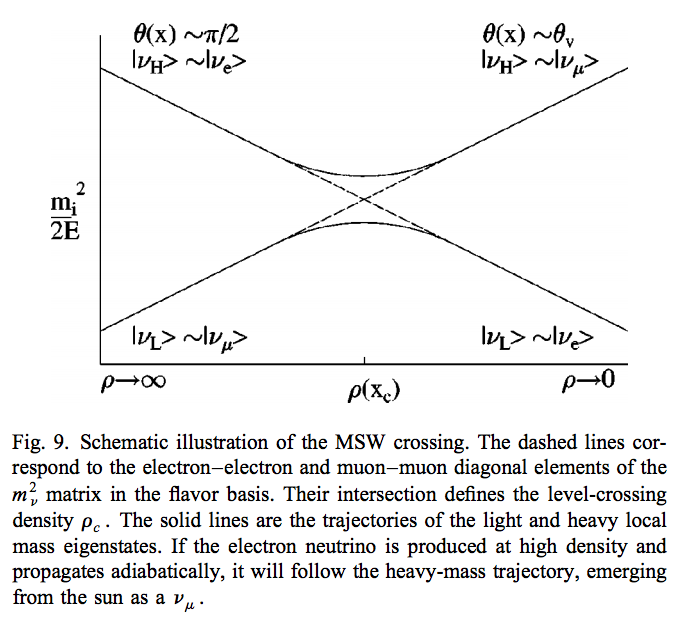
\includegraphics{msw.png}
\caption{\href{http://scitation.aip.org/content/aapt/journal/ajp/68/1/10.1119/1.19368}{Neutrino physics} by Wick C. Haxton and Barry R. Holstein.}\end{figure}

\index{MSW effect}

\section{MSW Refraction, Resonance and More}
\label{msw:msw-refraction-resonance-and-more}\label{msw:index-1}
\begin{notice}{note}{Hysteresis Loops of Neutrino Oscillations Due to MSW Effect}

Due to MSW effect, a system that is close to adiabaticity but not exactly adiabaticity could exhibit hysteresis effect, i.e., neutrinos going from high density region to low density region then coming back could form a hysteresis loop.
\end{notice}

TODO
\begin{enumerate}
\item {} 
Write down the effective potential \(V(x)\) which depends on the position. Refractive index is defined as \(n_{ref} - 1 = \frac{V}{p}\).

\item {} 
Two characteristic length: \(l_v = \frac{4\pi E}{ \Delta m^2 }\) as the vacuum oscillation length and \(l_0=\frac{2\pi}{V}\) as the refraction length. As the becomes comparable resonance occurs. For small mixing angle cases, resonance happens when vacuum length is about the length of refraction.

\end{enumerate}

There are three different matrix representatioins that is useful to the calculations.
\begin{enumerate}
\item {} 
Flavor basis;

\item {} 
Vacuum mass eigenstate basis;

\item {} 
Instataneous mass eigenstate basis.

\end{enumerate}

\begin{notice}{note}{Basis of Hamiltonian}

In vacuum mass eigenstate basis, the Hamiltonian without matter and self-interaction is easy and straightforward,
\begin{gather}
\begin{split}\mathbf{H_{vmv}} = \mathbf{H_{vp}} = \frac{1}{2E}\begin{pmatrix} m_1^2 & 0 & 0 \\ 0 & m_2^2 & 0  \\ 0 & 0 & m_3^2
\end{pmatrix}.\end{split}\notag
\end{gather}
To remove the trace, we can subtract a identity matrix
\begin{gather}
\begin{split}&\mathbf{H}- \frac{m_1^2}{2E}\mathbf{I} \\
=& \frac{1}{2E}\begin{pmatrix}
m_1^2 & 0 & 0 \\
0 & m_2^2 &  0\\
0 & 0 & m_3^2
\end{pmatrix} - \frac{m_1^2}{2E} \mathbf{I} \\
=& \frac{1}{2E} \begin{pmatrix}
0 & 0 & 0 \\
0 & \Delta m_{12}^2 & 0 \\
0 & 0 & \Delta m_{13}^2
\end{pmatrix}\end{split}\notag
\end{gather}
The interaction in flavor basis is
\begin{gather}
\begin{split}\mathbf{V_f} = \begin{pmatrix} \sqrt{2}G_F n & 0 & 0 \\ 0 & 0 & 0\\ 0 & 0 & 0 \end{pmatrix}.\end{split}\notag
\end{gather}
\textbf{To write down the Hamiltonian in vacuum mass eigenstates}, we transform the interaction term to vacuum mass eigenstates by
\begin{gather}
\begin{split}\mathbf{V_{vm}} = \mathbf{U^{-1}} \mathbf{V} \mathbf{U},\end{split}\notag
\end{gather}
where \(U\) is the PMNS matrix.

\textbf{To write down the Hamiltonian in flavor basis}, we transform the vacuum Hamiltonian to flavor basis \textbf{after remove the trace}, which is
\begin{gather}
\begin{split}\mathbf{H_{fv}} = \mathbf{U} \mathbf{H_{vmv}} \mathbf{U^{-1}}.\end{split}\notag
\end{gather}
\textbf{We could also write down the Hamiltonian matrix in instantaneous mass eigenstates}, which requires a instantaneous diagonalization.
\end{notice}

\index{solar neutrinos}

\subsection{2 Flavor Neutrino Oscillations and Matter Effect}
\label{msw:flavor-neutrino-oscillations-and-matter-effect}\label{msw:index-2}
\begin{notice}{note}{Solar Neutrinos}

Electron neutrinos are produced in the core of the sun then the neutrinos would propagate out to the surface of the sun without much difficulty. What is the predicted neutrino survival probability?
\end{notice}

Interaction with matter plays a big role in neutrino oscillation. As shown previously, the interaction only affects (anti) electron neutrinos. In other words, the interaction term in flavor basis is
\begin{gather}
\begin{split}V_f = \begin{pmatrix} \Delta & 0 \\ 0 & 0  \end{pmatrix}.\end{split}\notag
\end{gather}
where \(\Delta = \sqrt{2} G_F n\) and \(n\) is the number density of the electrons. However, to do calculations, since identity matrix doesn't change the survival probability, we can always make the hamiltonian traceless, which becomes
\begin{gather}
\begin{split}H_i=\frac{\Delta}{2} \boldsymbol{\sigma_3}.\end{split}\notag
\end{gather}

\subsection{Constant Electron Number Density}
\label{msw:constant-electron-number-density}
Suppose we have an environment with constant electron number density, the term \(- i \mathbf{U_m^{-1}} ( \partial_x \mathbf{U_m} )\) goes away. All we have is the diagonalized new Hamiltonian \(\mathbf{H_{md}}\) and the eigenvalues are easily obtained which are
\begin{gather}
\begin{split}E_1 &= A_3\cos 2\theta(x) - A_1 \sin 2\theta(x) \\
E_2 & = - A_3 \cos 2\theta(x) + A_1 \sin 2\theta(x) .\end{split}\notag
\end{gather}
The final result for these two eigenvalues are
\begin{gather}
\begin{split}E_1 &= -\sqrt{ \frac{\Delta^2 + \omega^2 }{4} - \frac{\Delta \omega }{2} \cos 2\theta_v. } \\
E_2 &= \sqrt{ \frac{\Delta^2 + \omega^2 }{4} - \frac{\Delta \omega }{2} \cos 2\theta_v. }.\end{split}\notag
\end{gather}
Meanwhile the eigenstates are denoted as \(\ket{\nu_{c1}}\) and \(\ket{\nu_{c2}}\).

\begin{notice}{note}{Two Special Cases}

Two special cases,
\begin{enumerate}
\item {} 
\(\cos 2\theta_v \to 0\);

\item {} 
\(\cos 2\theta_v \to 1\).

\end{enumerate}
\end{notice}

As for the survival probability for the initial condition that \(\Psi(x=0)=\ket{\nu_{c1}}\), the result has the same form as the vacuum case, which is
\begin{gather}
\begin{split}P_x(\nu_e,L) = 1 - \sin^2(2\theta_m)\sin^2\left( \frac{\omega_m L}{2} \right) ,\end{split}\notag
\end{gather}
where
\begin{gather}
\begin{split}\sin 2\theta(x)  = \frac{\omega\sin 2\theta_v}{\sqrt{ \omega^2+\Delta^2 - 2 \omega \Delta\cos 2\theta_v }}.\end{split}\notag
\end{gather}
\(\theta_m = \theta(x)\) is the effective mixing angle which in fact doesn't depend on \(x\) if the matter profile is constant.

\begin{notice}{note}{Vacuum Survival Probability}

As an comparison, the vacuum result is
\begin{gather}
\begin{split}P_x(\nu_e,L) = 1 - \sin^2(2\theta)\sin^2\left( \frac{\omega L}{2} \right) ,\end{split}\notag
\end{gather}
for all electron flavor initial condition.
\end{notice}


\subsection{Adiabatic Limit}
\label{msw:adiabatic-limit}
In some astrophysical environments the electron number density changes very slowly which means the term \(\mathbf{U_m^{-1}} \partial_x \mathbf{U_m}\) is much smaller than \(\mathbf{H_{md}}\). By intuition we would expect that this term could be dropped to the lowest order.

The eigen energies are slowing changing with the position of neutrinos,
\begin{gather}
\begin{split}E_1 & = -\frac{\omega}{2}\sqrt{\hat\Delta^2 + 1 - 2 \hat\Delta  \cos 2\theta_v} \\
E_2 & = \frac{\omega}{2}\sqrt{\hat\Delta^2 + 1 - 2 \hat\Delta  \cos 2\theta_v}.\end{split}\notag
\end{gather}
When the term \(\hat\Delta\) is very small \(1-2\hat\Delta\cos 2\theta_v\) will dominate and the whole term decreases. On the other hand as \(\hat\Delta\) becomes large, \(\hat\Delta^2\) will dominate and the whole term grows. Mathematically we could find the region when the part \(\sqrt{\hat\Delta^2 + 1 - 2 \hat\Delta  \cos 2\theta_v}\) decreases and increases.
\begin{figure}[htbp]
\centering
\capstart

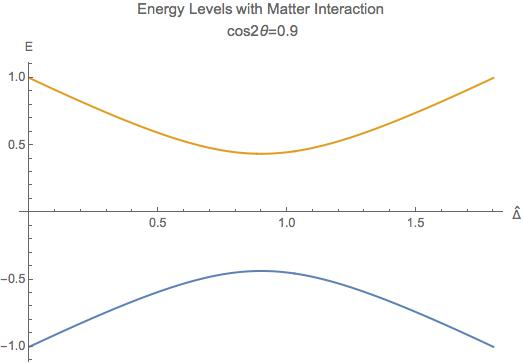
\includegraphics{mswEnergyLevels.jpg}
\caption{Energy Levels for MSW effect. We have the up-down symmetry since we shifted the energy by a constant to remove the identity matrix in the Hamiltonian.}\end{figure}

The survival probability for the light neutrinos would be
\begin{gather}
\begin{split}P_x(\nu_L,L) = 1 - \sin^2(2\theta (x))\sin^2\left( \frac{\omega L}{2} \right) .\end{split}\notag
\end{gather}
The survival probability for electron flavor neutrino is
\begin{gather}
\begin{split}P_x(\nu_e,L) = \frac{1}{2} + \frac{1}{2}\cos 2\theta(x_0) \cos 2\theta_v,\end{split}\notag
\end{gather}
if the neutrinos are produced in dense region and the detection happens in vacuum.

\begin{notice}{note}{Adiabatic Limit of Nuetrino Oscillations in Matter}

Before we move on to higher order corrections, it would be nice to understand this phenomenon.
\begin{enumerate}
\item {} 
The vacuum oscillation length can be extracted from vacuum oscillation survival probability. It is \(L_v = \frac{2\pi}{\omega}\).

\item {} 
In this problem we have another energy scale which is the interaction, \(\Delta\). Here we can define another characteristic length \(l_m = \frac{2\pi}{\Delta}\).

\item {} 
MSW resonance happens when the two character lengths are matching with each other. Another way to put it is that the term \(\sin 2\theta(x)\) is minimized so that we have the smallest energy gap which leads to \(\hat\Delta = \cos 2\theta_v\). Equivalently this is the relation

\end{enumerate}
\begin{gather}
\begin{split}l_0 = l_m\cos 2\theta_v.\end{split}\notag
\end{gather}\begin{enumerate}
\setcounter{enumi}{3}
\item {} 
At resonance, we have
\begin{gather}
\begin{split}\cos 2\theta(x) &= 1 \\
\sin 2\theta(x) &= 0.\end{split}\notag
\end{gather}
This is max mixing of the states which means that at the resonance point
\begin{gather}
\begin{split}\begin{pmatrix} \nu_L(x_{r}) \\ \nu_H(x_{r}) \end{pmatrix} = \frac{\sqrt{2}}{2}\begin{pmatrix} 1 & -1 \\ 1 & 1 \end{pmatrix} \begin{pmatrix}\nu_e \\ \nu_x \end{pmatrix}\end{split}\notag
\end{gather}
\item {} 
Resonance conditions corresponds to a resonance density which is given by
\begin{gather}
\begin{split}n_e(x) = \frac{\omega}{\sqrt{2}G_F } \cos 2\theta_v \equiv n_0(E,\Delta m^2) \cos 2\theta_v,\end{split}\notag
\end{gather}
where \(n_0(E,\Delta m^2)=\frac{\omega}{\sqrt{2}G_F }\) is a characteristic number density which depends on the energy mixing angles and \(\Delta m^2\) of the neutrinos.

\item {} 
One should notice that if the condition \(\sin^2 2\theta(x) = \sin^2 2\theta_v\) is satisfied, the survival probability for \(\ket{\nu_1}\) has the same \textbf{the form of} vacuum oscillation survival probability for electron neutrinos. The condition is solved,
\begin{gather}
\begin{split}\hat\Delta^2 + 1 - 2\hat\Delta \cos 2\theta_v = 1,\end{split}\notag
\end{gather}
which leads to
\begin{gather}
\begin{split}\hat\Delta = 0 \quad\text{or}\quad 2\cos 2\theta_v .\end{split}\notag
\end{gather}
The first condition is trivial which corresponds to vacuum however the second condition \(\Delta = 2\cos 2\theta_v \omega\) means the interaction oscillation length is doubled compared to resonance point.

\textbf{Nevertheless, we should always remember to check what survival probability the expression is describing. Here we have survival probability for} \(\nu_L(x)\). At \(n(x)\to 0\) the oscillation becomes vacuum oscillation.

\end{enumerate}
\end{notice}

\begin{notice}{note}{In The Basis of Vacuum Energy Eigenstates}

We could also using the basis of vacuum energy eigenstates, in which the vacuum part of the Hamiltonian is
\begin{gather}
\begin{split}\mathbf{H_{vmv}} = \frac{1}{2} \begin{pmatrix}
E_2 - E_1 & 0 \\
0 & E_2 - E_1
\end{pmatrix} \equiv  \frac{1}{2} \begin{pmatrix}
\Delta E & 0 \\
0 & \Delta E
\end{pmatrix} .\end{split}\notag
\end{gather}
The matter interaction in flavor basis is
\begin{gather}
\begin{split}\begin{pmatrix}
\Delta & 0 \\
0 & 0
\end{pmatrix}.\end{split}\notag
\end{gather}
It is more convinient to use the traceless potential
\begin{gather}
\begin{split}\mathbf{V_{f}} = \frac{\Delta}{2}\begin{pmatrix}
1 & 0 \\
0 & -1
\end{pmatrix}.\end{split}\notag
\end{gather}
Transform it to vacuum energy eigenstate basis, we have
\begin{gather}
\begin{split}\mathbf{V_{vm}} &= \mathbf{U^{-1}}\mathbf{V_{f}} \mathbf{U} \\
& = \Delta \begin{pmatrix}
\cos 2\theta_v & \sin 2\theta_v \\
\sin 2\theta_v  & - \cos 2\theta_v
\end{pmatrix}.\end{split}\notag
\end{gather}
The Hamiltonian in this problem becomes
\begin{gather}
\begin{split}\mathbf{H_{vm}} = \begin{pmatrix}
- \frac{\Delta m^2}{4E}+\cos 2\theta_v & \frac{\Delta}{2} \sin 2\theta_v \\
\frac{\Delta}{2} \sin 2\theta_v & \frac{\Delta m^2}{4E} -  \frac{\Delta}{2} \cos 2\theta_v
\end{pmatrix}.\end{split}\notag
\end{gather}\end{notice}


\subsection{General Discussion of Matter Effect}
\label{msw:general-discussion-of-matter-effect}
This part is a very general discussion of the matter effect \phantomsection\label{msw:id1}{\hyperref[msw:parke1986]{\emph{{[}Parke1986{]}}}}.

To work in flavor basis, we use the subscript \({}_{mf}\) to denote the flavor basis representation with mass effect. The equation of motion in flavor basis can be written down as
\begin{gather}
\begin{split}i\partial_x \Psi_{mf}(x) = \mathbf{H_{mf}} \Psi_{mf}(x)\end{split}\notag
\end{gather}
where
\begin{gather}
\begin{split}\mathbf{H_{mf}} =  \left(  \frac{\Delta}{2} -  \frac{\omega}{2} \cos 2\theta_v  \right) \boldsymbol{\sigma_3} + \frac{\omega}{2} \sin 2\theta_v \boldsymbol{\sigma_1}.\end{split}\notag
\end{gather}
There are three stages for neutrinos to travel from the core of the sun to vacuum.
\begin{enumerate}
\item {} 
At the core, electron neutrinos are produced. The electron flavor state should be projected onto heavy and light instantaneous mass eigenstates. What fallows is the that the propagation is adiabatic until the transition happens.
As we have seen in adiabatic situation, the states will stay in heavy and light states all along the evolution if the system starts from heavy or light state,
\begin{gather}
\begin{split}\ket{\nu_{a1}(x)} &= \exp(-i \int_0^x \frac{\omega_m(x)}{2} dx )  \ket{\nu_L(x)} \\
\ket{\nu_{a2}(x)} &= \exp(i\int_0^x \frac{\omega_m(x)}{2} dx) \ket{\nu_H(x)},\end{split}\notag
\end{gather}
where the heavy and light states are defined in the adiabatic situation previously. \textbf{This is what happens before the passing through of the resonance.}

\item {} 
At the resonance point, light instantaneous mass eigenstate has a probability to jump to the heavy state and vice versa.
When it comes to the resonance point which is non-adiabatic propagation, the transition between the states \(\ket{\nu_L}\to a_L \ket{\nu_L(x)} + a_H \ket{\nu_H(x)} \ket{\nu_1(x)}\) and \(\ket{\nu_H}\to b_L \ket{\nu_L(x)} + b_H \ket{\nu_H(x)}\) will mix the heavy and light state up.
\begin{gather}
\begin{split}\ket{\nu_1(x)} &= a_L \exp(-i \int_{x_r}^x \omega_m(x')/2 dx' )  \ket{\nu_L(x)} + a_H \exp(i\int_{x_r}^x \omega_m(x')/2 dx') \ket{\nu_H(x)}  \\
\ket{\nu_2(x)} &= b_L \exp(-i \int_{x_r}^x \omega_m(x')/2 dx' )  \ket{\nu_L(x)} + b_H \exp(i\int_{x_r}^x \omega_m(x')/2 dx') \ket{\nu_H(x)},\end{split}\notag
\end{gather}
where the relations between the constants are determined using the condition that \(\ket{\nu_1(x)}\) and \(\ket{\nu_2(x)}\) are orthonormal, which leads to the conclusion that
\begin{gather}
\begin{split}b_L &= -a_H^* \\
b_H &= a_L^* \\
\lvert a_L \rvert^2 &=  - \lvert a_H \rvert^2 .\end{split}\notag
\end{gather}
\item {} 
After the resonance point, the heavy and light states will continue on their adiabatic propagation.

\end{enumerate}

\begin{notice}{note}{Helpful Notes}

The relation between \(\theta_m\) and \(\theta_v\) is given by
\begin{gather}
\begin{split}\omega_m\sin 2\theta_m =  \omega \sin 2\theta_v.\end{split}\notag
\end{gather}\end{notice}

Electron neutrinos are produced in a dense region as \(\ket{\nu_e}\), which are partially transformed to other the other neutrinos due to matter and the resonance then it propagates as if it satisfies the adiabatic condition again. The initial state in terms of light and heavy state is
\begin{gather}
\begin{split}\ket{\Psi_{m}(x_0)} = \ket{\nu_e}= \cos \theta_m(x_0) \ket{\nu_L(x_0)} + \sin \theta_m(x_0) \ket{\nu_H(x_0)}.\end{split}\notag
\end{gather}
The final state right before the resonance is
\begin{gather}
\begin{split}\ket{\Psi_{m}(x_{r-})} = \cos\theta_m(x_{0}) \exp\left( -i \int_{x_0}^{x_{r-}} \frac{\omega_m(x)}{2} dx   \right) \ket{\nu_L(x_{r-})} + \sin\theta_m(x_{0}) \exp\left( i \int_{x_0}^{x_{r-}} \frac{\omega_m(x)}{2} dx \right) \ket{\nu_H(x_{r-})}\end{split}\notag
\end{gather}
After the resonance the state is described by the general jumping
\begin{gather}
\begin{split}\ket{\Psi_{m}(x)}= &  \cos\theta_m(x_0) \exp\left( -i \int_{x_0}^{x_{r-}} \frac{\omega_m(x)}{2} dx   \right)  \left(  a_L \exp( -i \int_{x_r}^x \frac{\omega_m(x')}{2}dx' ) \ket{\nu_L(x)}  + a_H \exp( i\int_{x_r}^x \frac{\omega_m(x')}{2}dx' ) \ket{\nu_H(x)}  \right)  \\
& + \sin\theta_m(x_{0}) \exp\left( i \int_{x_0}^{x_{r-}} \frac{\omega_m(x)}{2} dx \right)  \left(  -a_H^* \exp( -i \int_{x_r}^x \frac{\omega_m(x')}{2}dx' ) \ket{\nu_L(x)}  + a_L^* \exp( i\int_{x_r}^x \frac{\omega_m(x')}{2}dx' ) \ket{\nu_H(x)}  \right)\end{split}\notag
\end{gather}
in which the \(x_{r-}\) is actually \(x_r\) thus
\begin{gather}
\begin{split}\ket{\Psi_{m}(x)}= &  \cos\theta_m(x_0) \exp\left( -i \int_{x_0}^{x_{r}} \frac{\omega_m(x)}{2} dx   \right)  \left(  a_L \exp( -i \int_{x_r}^x \frac{\omega_m(x')}{2}dx' ) \ket{\nu_L(x)}  + a_H \exp( i\int_{x_r}^x \frac{\omega_m(x')}{2}dx' ) \ket{\nu_H(x)}  \right)  \\
& + \sin\theta_m(x_{0}) \exp\left( i \int_{x_0}^{x_{r-}} \frac{\omega_m(x)}{2} dx \right)  \left(  -a_H^* \exp( -i \int_{x_r}^x \frac{\omega_m(x')}{2}dx' ) \ket{\nu_L(x)}  + a_L^* \exp( i\int_{x_r}^x \frac{\omega_m(x')}{2}dx' ) \ket{\nu_H(x)}  \right)\end{split}\notag
\end{gather}
To calculate the survival probability it is easier to use flavor basis, hence we have another form of \(\ket{\Psi_m(x)}\) which is
\begin{gather}
\begin{split}\ket{\Psi_{m}(x)}= &  \left[ \cos\theta_m(x_0) \exp\left( -i \int_{x_0}^{x_{r}} \frac{\omega_m(x')}{2} dx'   \right)   a_L \exp( -i \int_{x_r}^x \frac{\omega_m(x')}{2}dx' ) \right. \\
&  \left. - \sin\theta_m(x_{0}) \exp\left( i \int_{x_0}^{x_{r-}} \frac{\omega_m(x')}{2} dx' \right)    a_H^* \exp( -i \int_{x_r}^x \frac{\omega_m(x')}{2}dx' )  \right] \ket{\nu_L(x)}\\
& + \left[  \cos\theta_m(x_0) \exp\left( -i \int_{x_0}^{x_{r}} \frac{\omega_m(x)}{2} dx   \right) a_H \exp( i\int_{x_r}^x \frac{\omega_m(x')}{2}dx' ) \right. \\
& \left. + \sin\theta_m(x_{0}) \exp\left( i \int_{x_0}^{x_{r-}} \frac{\omega_m(x)}{2} dx \right)   a_L^* \exp( i\int_{x_r}^x \frac{\omega_m(x')}{2}dx' ) \right]  \ket{\nu_H(x)} \\
=&  \left[ \cos\theta_m(x_0) \exp\left( -i \int_{x_0}^{x_{r}} \frac{\omega_m(x)}{2} dx   \right)   a_L \exp( -i \int_{x_r}^x \frac{\omega_m(x')}{2}dx' ) \right. \\
&  \left. - \sin\theta_m(x_{0}) \exp\left( i \int_{x_0}^{x_{r-}} \frac{\omega_m(x)}{2} dx \right)    a_H^* \exp( -i \int_{x_r}^x \frac{\omega_m(x')}{2}dx' )  \right] ( \cos\theta_m(x)\ket{\nu_e} - \sin\theta_m(x)\ket{\nu_x} )\\
& + \left[  \cos\theta_m(x_0) \exp\left( -i \int_{x_0}^{x_{r}} \frac{\omega_m(x)}{2} dx   \right) a_H \exp( i\int_{x_r}^x \frac{\omega_m(x')}{2}dx' ) \right. \\
& \left. + \sin\theta_m(x_{0}) \exp\left( i \int_{x_0}^{x_{r-}} \frac{\omega_m(x)}{2} dx \right)   a_L^* \exp( i\int_{x_r}^x \frac{\omega_m(x')}{2}dx' ) \right] ( \sin\theta_m(x)\ket{\nu_e} + \cos\theta_m(x)\ket{\nu_x})\end{split}\notag
\end{gather}
Since \(\cos\theta_m\), \(\sin\theta_m\) and \(\omega_m\) are real while \(a_L\) and \(a_H\) are complex, survival amplitude of electron neutrinos is given by
\begin{gather}
\begin{split}&\braket{\Psi_m(0)}{\Psi_m(x)} \\
= & \braket{\nu_e}{\Psi_m(x)} \\
= &  \left[ \cos\theta_m(x_0) \exp\left( -i \int_{x_0}^{x_{r}} \frac{\omega_m(x')}{2} dx'   \right)   a_L \exp( -i \int_{x_r}^x \frac{\omega_m(x')}{2}dx' ) \right. \\
&  \left. - \sin\theta_m(x_{0}) \exp\left( i \int_{x_0}^{x_{r}} \frac{\omega_m(x')}{2} dx' \right)    a_H^* \exp( -i \int_{x_r}^x \frac{\omega_m(x')}{2}dx' )  \right]  \cos\theta_m(x) \\
& + \left[  \cos\theta_m(x_0) \exp\left( -i \int_{x_0}^{x_{r}} \frac{\omega_m(x')}{2} dx'   \right) a_H \exp( i\int_{x_r}^x \frac{\omega_m(x')}{2}dx' ) \right. \\
& \left. + \sin\theta_m(x_{0}) \exp\left( i \int_{x_0}^{x_{r}} \frac{\omega_m(x')}{2} dx' \right)   a_L^* \exp( i\int_{x_r}^x \frac{\omega_m(x')}{2}dx' ) \right]  \sin\theta_m(x) \\
=& A_L \exp\left( -i \int_{x_r}^{x} \frac{\omega_m(x')}{2} dx'   \right) + A_H \exp\left( i\int_{x_r}^x \frac{\omega_m(x')}{2}dx' \right),\end{split}\notag
\end{gather}
where the coefficients are
\begin{gather}
\begin{split}A_L(x) & = \cos\theta_m(x) \left[ a_L\cos\theta_m(x_0) \exp\left(  -i\int_{x_0}^{x_r} \frac{\omega_m(x')}{2} dx' \right) - a_H^*\sin\theta_m(x_0) \exp\left( i \int_{x_0}^{x_r} \frac{\omega_m(x')}{2}dx' \right)  \right] \\
A_H(x) & = \sin\theta_m(x)  \left[ a_H \cos\theta_m(x_0) \exp\left( -i \int_{x_0}^{x_{r}} \frac{\omega_m(x')}{2} dx'   \right)   + a_L^*\sin\theta_m(x_{0}) \exp\left( i \int_{x_0}^{x_{r}} \frac{\omega_m(x')}{2} dx' \right)    \right]  .\end{split}\notag
\end{gather}
The detection is in a region where matter density is very small, thus we use \(x\to\infty\) which means the effective mixing angle becomes vacuum mixing angle. The probability is the square of the amplitude,
\begin{gather}
\begin{split}P(\nu_e,x) &= \lvert \braket{\Psi_m(0)}{\Psi_m(x)}  \rvert^2 \\
& = \lvert A_L(x) \exp\left( -i \int_{x_r}^{x} \frac{\omega_m(x')}{2} dx'   \right) + A_H(x) \exp\left( i\int_{x_r}^x \frac{\omega_m(x')}{2}dx' \right)  \rvert^2 \\
& = \lvert A_L(x) \rvert^2 + \lvert A_H(x) \rvert^2 + A_L^*(x) A_H(x) \exp(2i\phi) + A_H^*(x) A_L(x) \exp(-2i\phi) \\
& = \lvert A_L(x) \rvert^2 + \lvert A_H(x) \rvert^2 + 2 \mathbf{Re}( A_L^*(x) A_H(x) \exp(2i\phi) ),\end{split}\notag
\end{gather}
where \(\phi\) is defined as
\begin{gather}
\begin{split}\phi = \int_{x_r}^{x} \frac{\omega_m(x')}{2}dx'.\end{split}\notag
\end{gather}
Note that for any complex number \((a+ib)e^{i\phi} \equiv \rho e^{i\psi}\),
\begin{gather}
\begin{split}(a+ib)e^{i\phi} + c.c.=2 \rho \cos(\psi+\phi),\end{split}\notag
\end{gather}
which means that the previous result can be simplified to
\begin{gather}
\begin{split}P(\nu_e,x) &=  \lvert A_L(x) \rvert^2 + \lvert A_H(x) \rvert^2 + 2 \mathbf{Re}( A_L^*(x) A_H(x) \exp(2i\phi) ) \\
& =  \lvert A_L(x) \rvert^2 + \lvert A_H(x) \rvert^2 + 2 \lvert A_L^*(x) A_H(x) \rvert \cos\left( 2\phi + \psi_{LH} \right),\end{split}\notag
\end{gather}
with the definition that \(\psi_{LH}(x)\) is the argument of \(A_L^*(x)A_H(x)\).

However the coefficients \(a_L\) and \(a_H\) are still not known yet. The trick is to average over the detection and production position. The average over \(x\) removes the \(\cos\) term due to the dependent of \(x\) for \(\phi\) and averages \(\cos^2\theta_m(x)\) to \(\frac{1}{2}\), which results in
\begin{gather}
\begin{split}\langle P(\nu_e,x)\rangle_{x} =& \cos^2\theta_m(x) (\lvert a_H\rvert^2 \cos^2\theta_m(x_0) + \lvert a_L\rvert^2 \sin^2\theta_m(x_0) ) \\
& + \sin^2\theta_m(x) ( \lvert a_H\rvert^2 \cos^2\theta_m(x_0) + \lvert a_L \rvert^2 \sin^2\theta_m(x_0) ) \\
& + ( - \cos^2\theta_m(x) + \sin^2\theta_m(x) ) \cos\theta_m(x_0)\sin\theta_m(x_0) ( a_H a_L e^{-2i\phi'} + \mathrm{c.c}) .\end{split}\notag
\end{gather}
Applying the condition that \(\lvert a_L \rvert^2 + \lvert a_H \rvert^2 = 1\), the probability becomes
\begin{gather}
\begin{split}\langle P(\nu_e,x)\rangle_{x} =& \frac{1}{2} + \frac{1}{2} (1 - 2 \lvert a_H \rvert^2) \cos 2\theta_m(x_0) \cos 2\theta_v - \lvert a_H a_L \rvert \sin 2\theta_m(x_0)\cos 2\theta_v \cos ( 2 \phi' + \psi_{LH} ),\end{split}\notag
\end{gather}
where \(\psi_{LH}\) is the argument of \(a_H a_L\) and \(\phi\) is \(\int_{x_0}^{x_r} \frac{\omega_m(x')}{2}dx'\) .

\textbf{The average over production removes the last part.}

Notice that in fact the detection happens in vacuum, which means \(\theta_m(x)=\theta_v\).
\begin{gather}
\begin{split}\langle \langle P(\nu_e,x)\rangle_{x} \rangle_{x_0}= \frac{1}{2} + \frac{1}{2}(1- 2\lvert a_H \rvert^2) \cos 2\theta_m(x_0) \cos 2\theta_v .\end{split}\notag
\end{gather}
\textbf{This means that the adiabatic result is of the form}
\begin{gather}
\begin{split}P(\nu_e,x)_{\mathrm{adiabatic}} = \frac{1}{2} ( 1+ \cos 2\theta_m \cos 2\theta_v ).\end{split}\notag
\end{gather}
Define a transition probability at resonance
\begin{gather}
\begin{split}P_r(\nu_L \to \nu_H) = \lvert a_2 \rvert^2,\end{split}\notag
\end{gather}
which can be determined by the Landau-Zener transition analytically (first order) to the first order.

\index{Landau-Zener Transition}

\subsection{Landau-Zener Transition of Neutrinos}
\label{msw:landau-zener-transition-of-neutrinos}\label{msw:index-3}
As discussed in the previous subsection, a transition probability between the two states \(\ket{\nu_L(x)}\) and \(\ket{\nu_H(x)}\) would change the final survival probabilty. Thus calculating this transition probability will be done in this subsection.

Recall that the effective potential is
\begin{gather}
\begin{split}\mathbf{V_m} & = -i\mathbf{U_m^{-1}} ( \partial_x \mathbf{U_m} ) ,\end{split}\notag
\end{gather}
where
\begin{gather}
\begin{split}\mathbf{U_m} = \begin{pmatrix} \cos \theta(x) & \sin\theta(x) \\ -\sin\theta(x) & \cos\theta(x) \end{pmatrix} .\end{split}\notag
\end{gather}
\(\sin\theta(x)\) and \(\cos\theta(x)\) can be found by solving the equations. Plug in the results and applying the trick that
\begin{gather}
\begin{split}\partial_x \mathbf{U_m} & = \frac{d \hat\Delta(x)}{dx} \partial_{ \hat\Delta(x)} \mathbf{U_m} ,\end{split}\notag
\end{gather}
we have
\begin{gather}
\begin{split}\mathbf{V_m} & = -i\mathbf{U_m^{-1}} ( \partial_x \mathbf{U_m} ) \\
& = - i \frac{\hat\Delta'(x_r) \sin 2\theta_v}{ 1 + 2 (\hat\Delta(x)-\cos 2\theta_v)^2 - \cos 4\theta_v }   \begin{pmatrix}
0 & 1 \\
-1 & 0
\end{pmatrix} .\end{split}\notag
\end{gather}
Since we are dealing with resonance which is located at \(\hat\Delta =\cos 2\theta_v\), the quantities can be expanded around \(\hat\Delta - \cos 2\theta = 0\).

To keep only first order of in the effective potential, we have to expand around \(\hat\Delta = \cos 2\theta_v\)
\begin{gather}
\begin{split}\mathbf{V_m(x)} & = - i \hat\Delta'(x_r) \frac{\sin 2\theta_v}{4(\cos 2\theta_v -1)} \left( -1 + (\hat\Delta(x) - 1)  \right)  \begin{pmatrix}
0 & 1 \\
-1 & 0
\end{pmatrix}.\end{split}\notag
\end{gather}
\begin{notice}{note}{Pauli Matrices}

The effective potential can be written in terms of \(\sigma_2\),
\begin{gather}
\begin{split}\sigma_2 = - i  \begin{pmatrix}
0 & 1 \\
-1 & 0
\end{pmatrix}.\end{split}\notag
\end{gather}\end{notice}

The equation of motion up to first order of \(\hat\Delta\) becomes
\begin{gather}
\begin{split}i\partial_x\ket{\Psi_m} = (\mathbf{H_{md}} + \mathbf{V_m})\ket{\Psi_m}.\end{split}\notag
\end{gather}
We have already solved
\begin{gather}
\begin{split}i\partial_x\ket{\Psi_m} = \mathbf{H_{md}} \ket{\Psi_m},\end{split}\notag
\end{gather}
where the eigenstates are \(\ket{\nu_L}\) and \(\ket{\nu_H}\) with eigenvalues \(\omega_{m1}\) and \(\omega_{m2}\) respectively.

To save typing we define
\begin{gather}
\begin{split}v &= -  \hat\Delta'(x_r) \frac{1}{2\sin 2\theta}\end{split}\notag
\end{gather}
so that the effective potential reduces to a simple form
\begin{gather}
\begin{split}\mathbf{V_m} = \begin{pmatrix}
0 & i v \\
-i v & 0
\end{pmatrix}.\end{split}\notag
\end{gather}
The general solution to the equation we need to solve can be written as
\begin{gather}
\begin{split}\ket{\Psi_m} = C_L(x) e^{-i\int \omega_{m1} dx} \ket{\nu_L} + C_H(x) e^{-i\int \omega_{m2} dx} \ket{\nu_H},\end{split}\notag
\end{gather}
where
\begin{gather}
\begin{split}\omega_{m1} &=-\sqrt{ \frac{\Delta^2 + \omega^2}{4}-\frac{\Delta \omega}{2} \cos 2\theta_v } \\
& = -\omega \sqrt{\left( \frac{\hat\Delta^2 + 1}{4} - \frac{\hat\Delta}{2}\cos 2\theta_v \right)} , \\
\omega_{m2} & = - \omega_{m1} \equiv \frac{\omega_m}{2}.\end{split}\notag
\end{gather}
Hamiltonian applied to this state results in
\begin{gather}
\begin{split}\mathbf{H_m} \ket{\Psi_m} =& \omega_{m1} C_L(x) e^{-i\int \omega_{m1}dx} \ket{\nu_L} -ivC_L(x) e^{-i\int \omega_{m1}dx}\ket{\nu_H} \\ &+\omega_{m2}C_H(x) e^{-i\int \omega_{m2}dx}\ket{\nu_H} + iv C_H(x) e^{-i\int \omega_{m2}dx}\ket{\nu_L}.\end{split}\notag
\end{gather}
Plug the state \(\ket{\Psi_m}\) into the Schrodinger equation, we have
\begin{gather}
\begin{split}\dot C_L(x) &= v C_H(x) e^{  i\int  \omega_m dx} \\
\dot C_H(x) & = -v C_L(x) e^{ - i\int \omega_m dx} ,\end{split}\notag
\end{gather}
in which \(omega_m\) is
\begin{gather}
\begin{split}\omega_m =  \omega_{m2} - \omega_{m1} = 2\omega_{m2} = \omega\sqrt{ \hat\Delta^2 + 1 - 2 \hat\Delta \cos 2\theta_v } .\end{split}\notag
\end{gather}
The boundary condition for such a problem \textbf{in general} is
\begin{gather}
\begin{split}\ket{\Psi_m(0)} = C_L(0)\ket{\nu_L} + C_H(0) \ket{\nu_H}.\end{split}\notag
\end{gather}
\textbf{It should be made clear that the problem we will be discussing is the transition from one state} \(\ket{\nu_L(x)}\) \textbf{to another} \(\ket{\nu_H(x)}\) \textbf{in first order approximation. That means we will confine this system so that the initial condition is} \(\ket{\Psi_m(-\infty)} = \ket{\nu_L}\). In terms of \(C_L\) and \(C_H\),
\begin{gather}
\begin{split}C_L(-\infty) &= 0, \\
\lvert C_H(-\infty) \rvert^2 & = 1.\end{split}\notag
\end{gather}
The first order differential equations of \(C_L(x)\) and \(C_H(x)\) can be combined and produce a second order differential equation.
\begin{gather}
\begin{split}\ddot C_L - \left(   \frac{\dot v}{v} + i\omega_m \right) \dot C_L + v^2 C_L = 0.\end{split}\notag
\end{gather}
\textbf{If we use the approximation that} \(\frac{d \hat\Delta }{dx}\) \textbf{is a constant, where in fact we are assuming that} \(n(x)\) \textbf{is linearly depending on} \(x\) \textbf{which means} \(\hat\Delta\) \textbf{is a linear function of} \(x\). \textbf{Thus} \(v\propto\frac{d\hat\Delta}{dx}\) \textbf{is a constant.} The equation simplifies to
\begin{gather}
\begin{split}\ddot C_L - i\omega_m \dot C_L + v^2 C_L = 0,\end{split}\notag
\end{gather}
where \(v=-\frac{\cot\theta_v}{4} \frac{d\hat\Delta}{dx}\) is constant.

\textbf{In the paper by Zener,} \phantomsection\label{msw:id2}{\hyperref[msw:zener1932]{\emph{{[}Zener1932{]}}}} we need to do substitution of the function \(C_L\) so that the equation reduces to Weber equation.

The eigenvalues are not varying very fast and satisfies the condition that
\begin{gather}
\begin{split}\omega_m(x) =  \omega_m(x_r) +  \alpha (x-x_r),\end{split}\notag
\end{gather}
where \(\alpha = \delta \omega_m'(x_r)\) is a constant and comes from the first order of the expression.

Define a new variable \(W\) which is determined by

\begin{notice}{note}{The Trick}

This is done by assuming \(C_L=f(x)W\) and plugging it back to the equation then set the coefficient of \(\dot C_L\) to \(0\).\}
\end{notice}
\begin{gather}
\begin{split}C_L = e^{ \frac{i}{2}\int \delta \omega_m dx' } W.\end{split}\notag
\end{gather}
Then we get a simple equation about \(W\),
\begin{gather}
\begin{split}\ddot W + \left( v^2 + \frac{i \alpha}{2} + \frac{\alpha^2 }{4} (x - x_r + \frac{2\sin\theta_v}{\alpha})^2  \right) W = 0,\end{split}\notag
\end{gather}
which can be reduced to the standard form of Weber equation with the new parameters which are are found by using a single assumption that \(z=g(x- x_r + \frac{2\sin\theta_v}{\alpha})\),
\begin{gather}
\begin{split}z &= g \left(x - x_r + \frac{2\sin\theta_v}{ \alpha'} \right) \\
\nu &= i \frac{v^2}{\alpha'},\end{split}\notag
\end{gather}
where \(g^2\equiv -i\alpha'\) ( \(g=(1-i)\sqrt{\left\vert \alpha' \right\vert } /\sqrt{2}=\sqrt{\left\vert \alpha' \right\vert }e^{-i\pi/4}\) ) and \(\alpha' = -\alpha\). The equation we need to solve becomes
\begin{gather}
\begin{split}\frac{d^2 W(z)}{dz^2} + \left( \nu +\frac{1}{2} - \frac{1}{4}z^2 \right) W(z) = 0 .\end{split}\notag
\end{gather}
\begin{notice}{note}{Parabolic Cylinder Function}
\begin{figure}[htbp]
\centering
\capstart

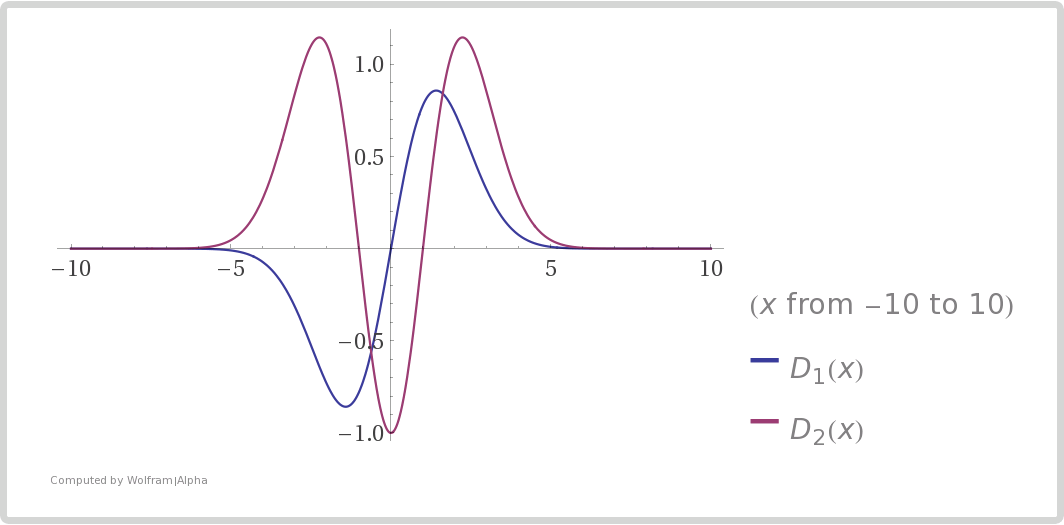
\includegraphics{weber1.png}
\caption{The parabolic cylinder function \(D_\nu(z)\) for \(\nu=1\) (blue) and \(\nu=2\) (red). But for imaginary \(z\) the function blows up.}\end{figure}

The Weber equation has two independent solutions \(D_\nu(z)\) and \(D_{-\nu-1}(iz)\). They are also called Parabolic Cylinder Function on \href{http://mathworld.wolfram.com/ParabolicCylinderFunction.html}{wolfram mathworld}.

Since \(D_{\nu}(z)\) blows up for the line on complex plane \(z\propto e^{-\pi i/4}\), the solution that works is \(D_{-\nu-1}(iz)\). Then the solution to \(U_L\) is
\begin{gather}
\begin{split}U_L(x) = u_{+} D_{-iv^2/\alpha -1} (\frac{1-i}{\sqrt{2}} x) ,\end{split}\notag
\end{gather}
or
\begin{gather}
\begin{split}U_L(x) = u_- D_{-iv^2/\alpha -1} ( - \frac{1-i}{\sqrt{2}} x) .\end{split}\notag
\end{gather}
The asymptotic expression for \(D_{-\nu-1}\) on the line of \(e^{-i\pi/4}\) and \(e^{-3i\pi/4}\) at infinite contour radius on complex plane are
\begin{gather}
\begin{split}D_{-\nu-1}(i x e^{-3i\pi/4}) &\to e^{i(\nu+1)\pi/4} e^{i x^2/4} x^{-\nu-1} \\
D_{-\nu-1}(i x e^{-i\pi/4}) &\to e^{-i(\nu+1)\pi/4} e^{-i x^2/4} x^{-\nu-1}.\end{split}\notag
\end{gather}
So the real part of these asymptotic expressions are
\begin{gather}
\begin{split}e^{i\nu\pi/4} x^{-\nu-1} &= e^{-v^2\pi/4\alpha'} x^{-\nu-1} \\
e^{-i\nu\pi/4} x^{-\nu-1} &=e^{v^2\pi/4\alpha'} x^{-\nu-1}\end{split}\notag
\end{gather}
Apply the boundary condition we have the results of the coefficients.
\begin{gather}
\begin{split}\lvert u_+ \rvert = \lvert u_- \rvert = e^{-\gamma \pi/4}\sqrt{\gamma} ,\end{split}\notag
\end{gather}
where \(\gamma = \frac{v^2}{\lvert \alpha \rvert}\).

What we need to find out is the state at \(x\to \infty\), which depends on the asymptotic values of \(D_{-\nu-1}\),
\begin{gather}
\begin{split}C_L(x) &\to \sqrt{\gamma} e^{-\gamma \pi/4} \left(  e^{3\pi (\nu+1)i/4} e^{-ix'^2/4} x'^{-\nu-1} + \frac{\sqrt{2\pi}}{ \Gamma (\nu+1) } e^{i \pi\nu/4} e^{i x'^2 /4} x'^\nu  \right) ,\end{split}\notag
\end{gather}
or
\begin{gather}
\begin{split}C_L & \to \sqrt{\gamma} e^{-\gamma \pi/4} \left(   e^{-3\pi (\nu+1)i/4} e^{ix'^2/4} x'^{-\nu-1} + \frac{\sqrt{2\pi}}{ \Gamma (\nu+1) } e^{i \pi\nu/4} e^{ - i x'^2 /4} x'^\nu   \right).\end{split}\notag
\end{gather}
The transition rate is determined by \(\lvert C_L \rvert^2\)
\begin{gather}
\begin{split}\lvert C_L(\infty) \rvert^2 = \gamma e^{-\pi\gamma} \frac{2\pi}{\Gamma(i\gamma +1) \Gamma(-i\gamma +1)} = 2e^{-\pi\gamma}\sinh \pi\gamma = 1-e^{-2\pi\gamma}.\end{split}\notag
\end{gather}
Now we understand the transition probability is given by
\begin{gather}
\begin{split}P_{tran} = e^{-2\pi\gamma}.\end{split}\notag
\end{gather}\end{notice}

Suppose we have the initial condition as \(\ket{\Psi_m(x=-\infty)} = \ket{\nu_L}\), the system can jump to \(\ket{\nu_H}\) since the state at arbitrary position \(x\) is a mixing of the two states. The probability of jumping is given by \phantomsection\label{msw:id3}{\hyperref[msw:sjparke1986]{\emph{{[}SJParke1986{]}}}} \phantomsection\label{msw:id4}{\hyperref[msw:petcov1987]{\emph{{[}Petcov1987{]}}}}
\begin{gather}
\begin{split}P(x\to \infty, \ket{\nu_L}\to\ket{\nu_H}) = \exp \left( -\frac{\pi}{2}\frac{\sin^2 2\theta_v}{\cos 2\theta_v} \frac{\omega}{\left\vert  \frac{d\hat\Delta}{dx} \right\vert_{x_r} } \right)\end{split}\notag
\end{gather}
The survival probability can be calculated by applying this transition probability to the result we had previously.

\textbf{To be clear, if electron neutrinos are produced inside core of our sun, it will be almost the heavy state.} Since the interaction with matter is very strong, it transfers to \(\ket{\nu_L}\) with probability \(P(x\to \infty, \ket{\nu_L}\to\ket{\nu_H})\) due to the gradient of the matter profile which works as the perturbation. Thus the final state will be a mixing of \(\ket{\nu_L}\) and \(\ket{\nu_H}\).


\section{Numerical Results}
\label{msw:numerical-results}

\subsection{2 Flavor Oscillation}
\label{msw:flavor-oscillation}
The equation of motion in flavor basis is
\begin{gather}
\begin{split}i\partial_x \Psi_{mf}(x) = \mathbf{H_{mf}} \Psi_{mf}(x)\end{split}\notag
\end{gather}
where
\begin{gather}
\begin{split}\mathbf{H_{mf}} =  \left(  \frac{\Delta}{2} -  \frac{\omega}{2} \cos 2\theta_v  \right) \boldsymbol{\sigma_3} + \frac{\omega}{2} \sin 2\theta_v \boldsymbol{\sigma_1}.\end{split}\notag
\end{gather}
Writing down the dimensionless equation, we have
\begin{gather}
\begin{split}i \partial_{\hat x} \Psi_{mf} = \frac{R_S \omega}{2} ( (\hat\Delta - \cos 2\theta_v ) \boldsymbol{\sigma_3} + \sin 2\theta_v \boldsymbol{\sigma_1} )  \Psi_{mf} .\end{split}\notag
\end{gather}
As for the data of the sun I use a simple exponential distribution. The data is also from the paper by Bahcall. The model using just exponential is not accurate however it is enough to make the point in MSW resonance. So I choose a solar model in which the core density is \(n(0) = 10^{-13}\mathrm{GeV}^{3}\). The distribution is
\begin{gather}
\begin{split}n =  10^{-13 - 4.3\hat x} \mathrm{GeV}^{3}.\end{split}\notag
\end{gather}
The numerical results can be obtains by plugging this density profile into the differential equation solver.
\begin{figure}[htbp]
\centering
\capstart

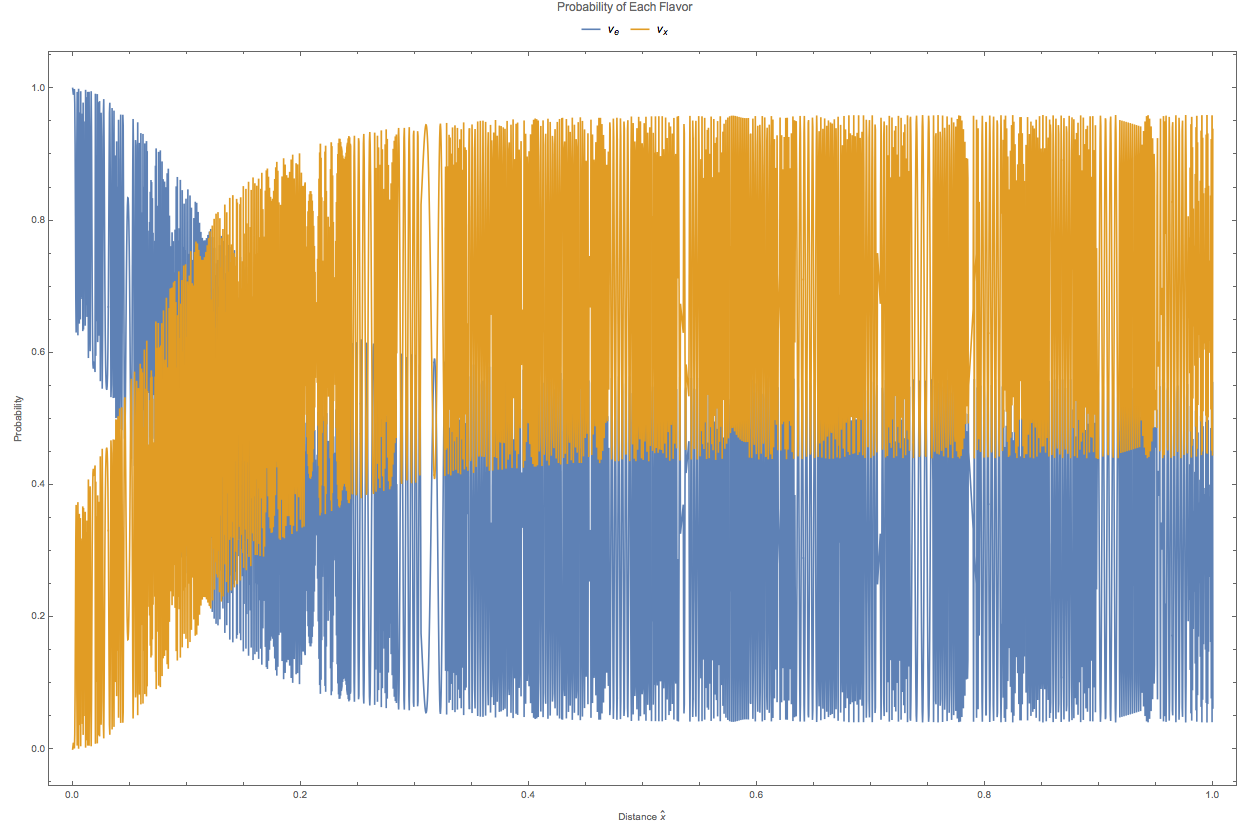
\includegraphics{numericalMSW-model-3.png}
\caption{Numerical results for electron flavor neutrino probability and the other flavor neutrino probability when the electron density profile is \(10^{-14 - 4.3\hat x} \mathrm{GeV}^{3}\).}\end{figure}
\begin{figure}[htbp]
\centering
\capstart

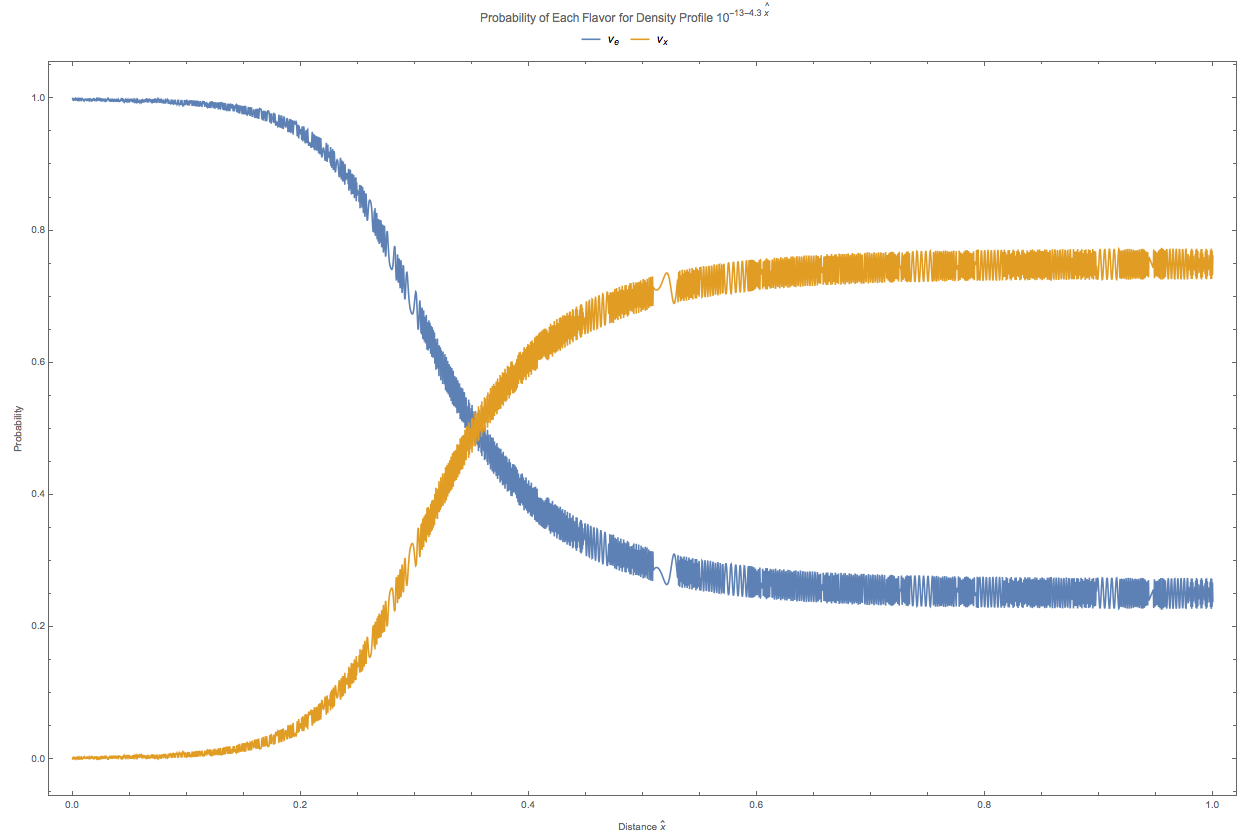
\includegraphics{numericalMSW-model-2flavor-minus13-1.png}
\caption{Number density profile \(n(\hat x) =  10^{-13 - 4.3\hat x}\mathrm{GeV^{3}}\).}\end{figure}

Since we can easily predict the survival probability using simple theory. Here are some comparision. The following figures are for matter profile \(10^{-13-4.3\hat x}\mathrm{GeV^3}\) and vacuum oscillation frequency \(\omega = 10^{-20} \mathrm{GeV}, 10^{-19} \mathrm{GeV},10^{-18} \mathrm{GeV},10^{-17} \mathrm{GeV}\) respectively. As we can see that in this two flavor special case, the problem doesn't dependent on energy and mass difference independently but depends only on \(\omega=\frac{\Delta m^2}{2E}\). If we choose \(\Delta m^2=7.5\times 10^{-5}\mathrm{eV^2}\), the four figures are corresponding to energies \(7.5\mathrm{MeV},0.75\mathrm{MeV},7.5\times 10^{-2}\mathrm{MeV},7.5\times 10^{-3}\mathrm{MeV}\).
\begin{figure}[htbp]
\centering
\capstart

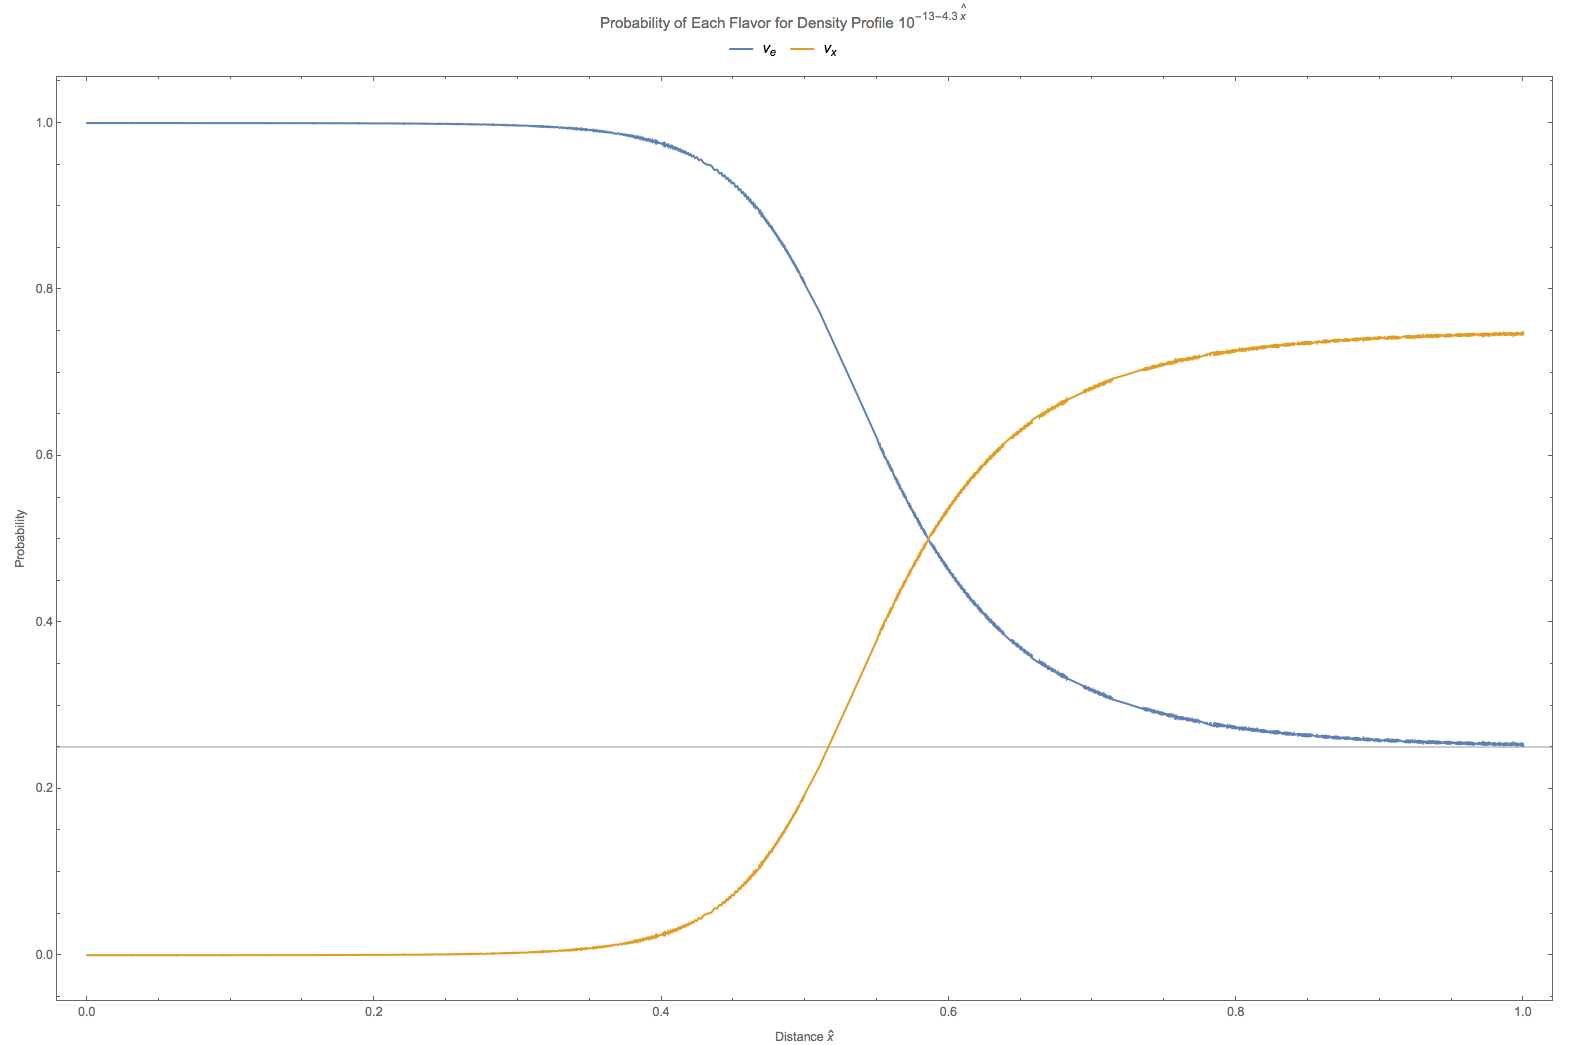
\includegraphics{compThNu13-1.png}
\caption{The grey line is theoretical survival probability at \(\hat x = 1\). In this calculation the vacuum oscillation frequency is set to \(\omega = 10^{-20} \mathrm{GeV}\).}\end{figure}
\begin{figure}[htbp]
\centering
\capstart

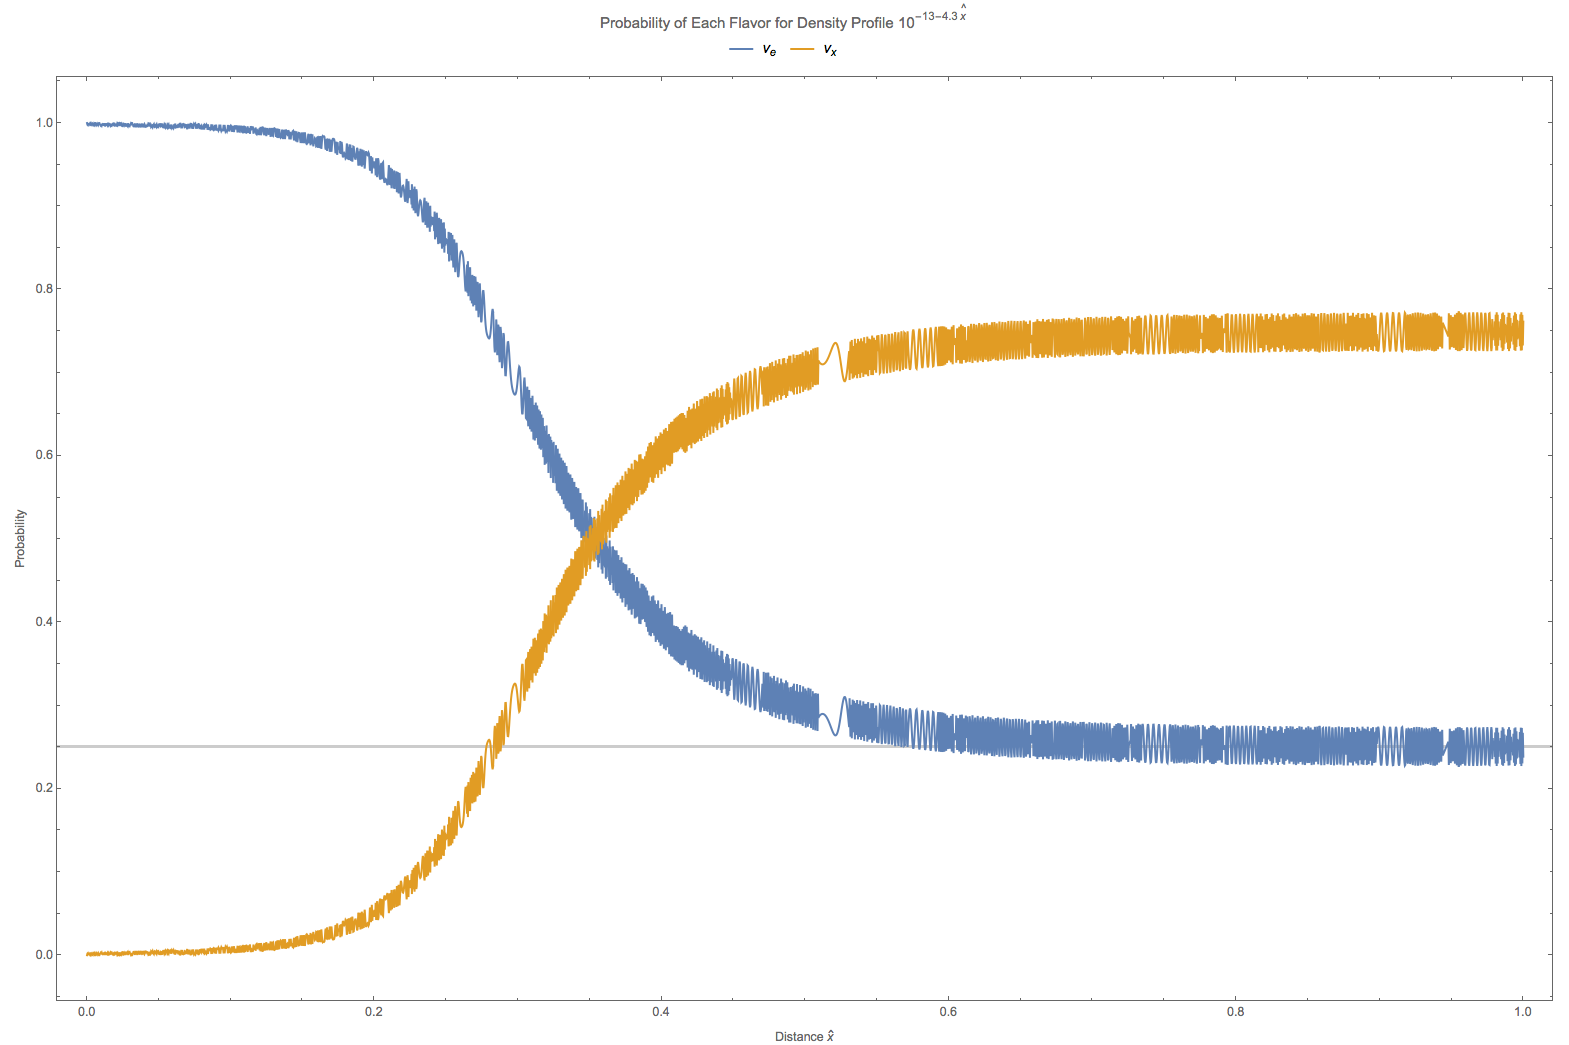
\includegraphics{compThNu13-2.png}
\caption{The grey line is theoretical survival probability at \(\hat x = 1\). In this calculation the vacuum oscillation frequency is set to \(\omega = 10^{-19} \mathrm{GeV}\).}\end{figure}
\begin{figure}[htbp]
\centering
\capstart

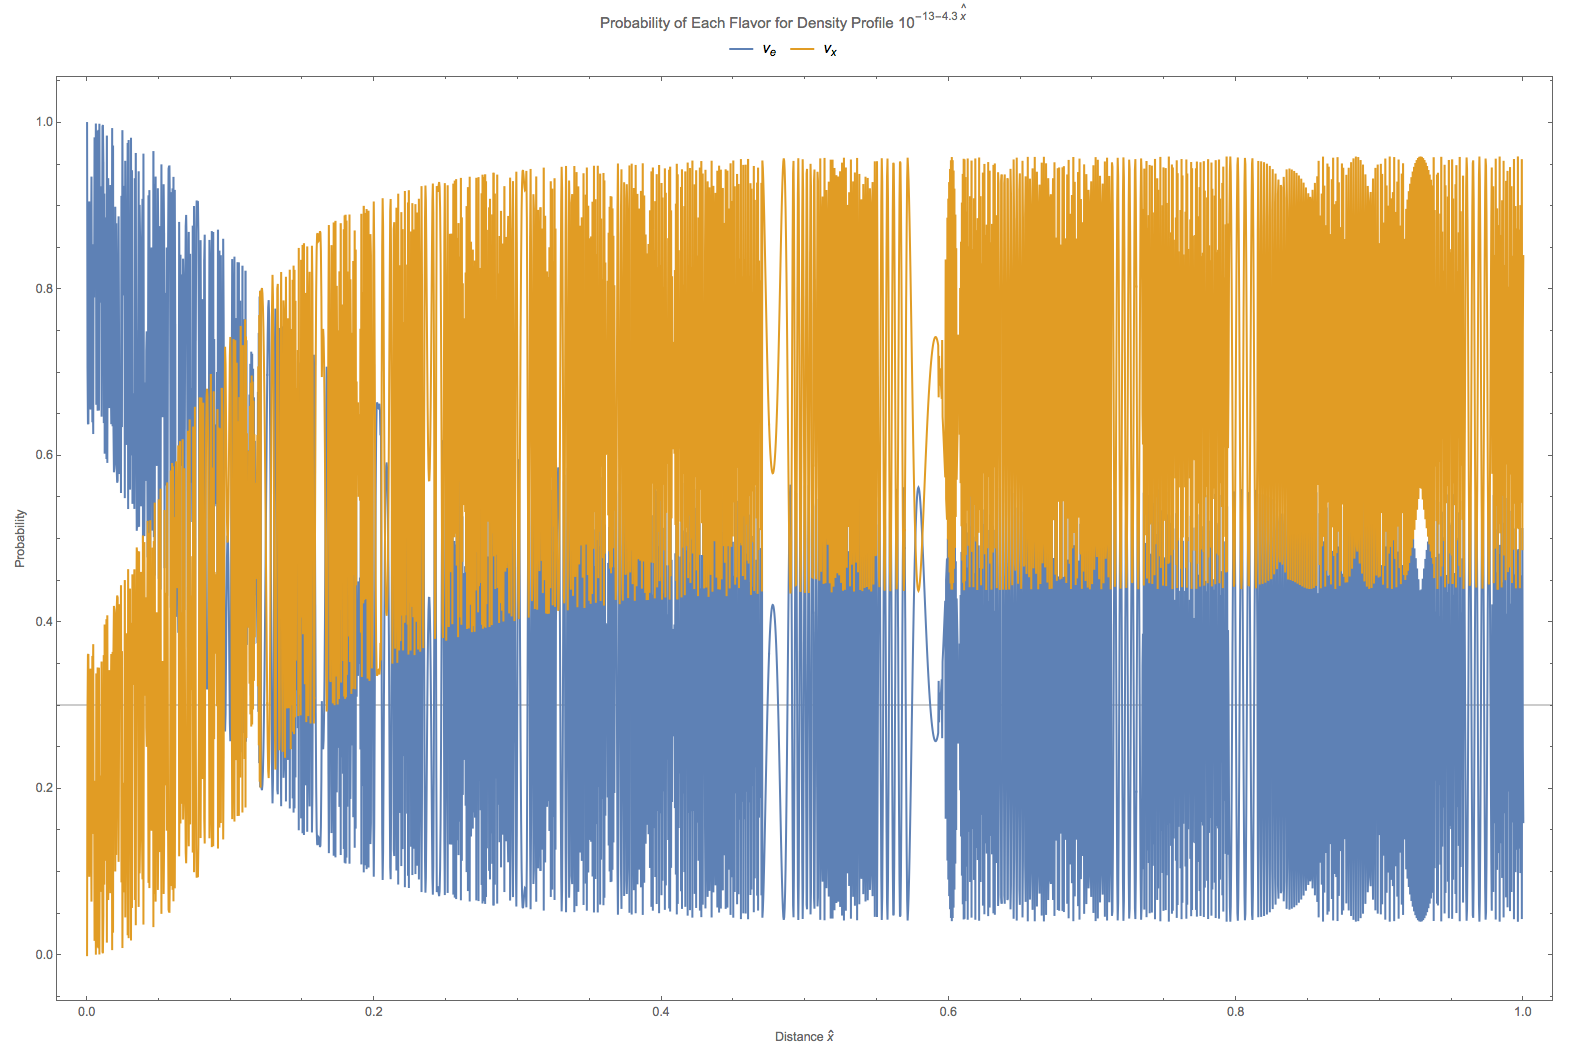
\includegraphics{compThNu13-3.png}
\caption{The grey line is theoretical survival probability at \(\hat x = 1\). In this calculation the vacuum oscillation frequency is set to \(\omega = 10^{-18} \mathrm{GeV}\).}\end{figure}
\begin{figure}[htbp]
\centering
\capstart

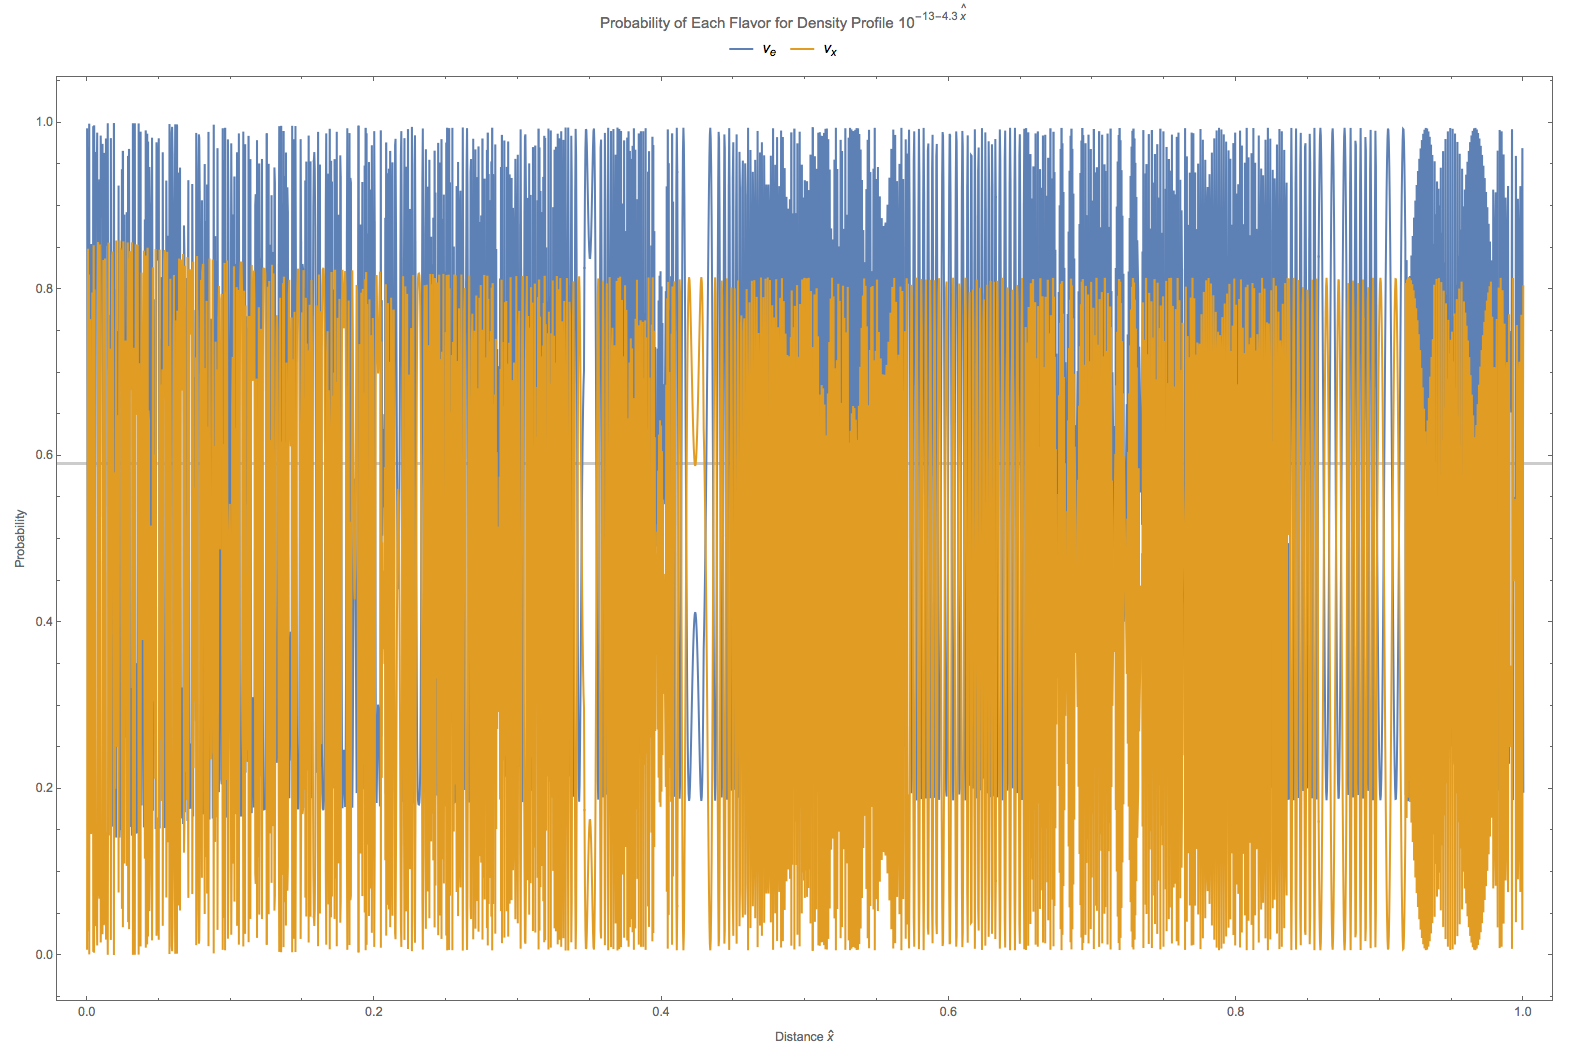
\includegraphics{compThNu13-4.png}
\caption{The grey line is theoretical survival probability at \(\hat x = 1\). In this calculation the vacuum oscillation frequency is set to \(\omega = 10^{-17} \mathrm{GeV}\).}\end{figure}


\subsection{Three flavor Oscillations}
\label{msw:three-flavor-oscillations}
Vacuum part of the Hamiltonian is
\begin{gather}
\begin{split}\mathbf{H_{mvv}} = \frac{1}{2E} \begin{pmatrix}
m_1^2 & 0 & 0 \\
0 & m_2^2 & 0 \\
0 & 0 & m_3^2
\end{pmatrix}.\end{split}\notag
\end{gather}
The matter interaction in flavor basis is
\begin{gather}
\begin{split}\mathbf{V_{mf}} = \sqrt{2}G_F n \mathrm{diag}{1,0,0}.\end{split}\notag
\end{gather}
Thus to work in vacuum mass eigenstates, we need a transformation
\begin{gather}
\begin{split}\mathbf{V_{mv}} = \mathbf{U^{-1}}\mathbf{V_{mf}} \mathbf{U}.\end{split}\notag
\end{gather}
Then the Hamiltonian becomes
\begin{gather}
\begin{split}\mathbf{H_{m}} = \begin{pmatrix}
\frac{m_1^2}{2E} + \Delta U_{e1}^2 & \Delta U_{e1} U_{e2} & \Delta U_{e1} U_{e3} \\
\Delta U_{e2} U_{e1} & \frac{m_2^2}{2E} + \Delta U_{e2}^2 & \Delta U_{e2} U_{e3} \\
\Delta U_{e3} U_{e1} & \Delta U_{e3} U_{e2} & \frac{m_3^2}{2E} + \Delta U_{e3}^2
\end{pmatrix}\end{split}\notag
\end{gather}
Trace of this Hamiltonian is \(\mathrm{Tr}(\mathbf{H_m}) = \frac{m_1^2+m_2^2+m_3^2}{2E}+\Delta\). To find the traceless part, we can use the relation \phantomsection\label{msw:id5}{\hyperref[msw:ohlsson2000]{\emph{{[}ohlsson2000{]}}}}
\begin{gather}
\begin{split}M = M_{traceless}+ \frac{1}{N} \mathrm{Tr}(M) I,\end{split}\notag
\end{gather}
where \(N\) is the rank.

The traceless part of Hamiltonian becomes
\begin{gather}
\begin{split}\mathbf{H_{m}} = \begin{pmatrix}
\Delta U_{e1}^2 - \frac{1}{3}\Delta + \frac{1}{3}(\frac{m_1^2-m_2^2 + m_1^2-m_3^2}{2E}) & \Delta U_{e1}U_{e2} & \Delta U_{e1} U_{e3} \\
\Delta U_{e2} U_{e1} & \Delta U_{e2}^2 -\frac{1}{3}\Delta + \frac{1}{3}\frac{m_2^2 - m_1^2+m_2^2-m_3^2}{2E} & \Delta U_{e2}U_{e3} \\
\Delta U_{e1} U_{e3} & \Delta U_{e2} U_{e3} & \Delta U_{e3}^2 -\frac{1}{3} \Delta + \frac{1}{3} \frac{m_3^2 - m_1^2 + m_3^2-m_2^2 }{2E}
\end{pmatrix}.\end{split}\notag
\end{gather}
Define the following quantities where only two of them are linearly independent
\begin{gather}
\begin{split}\Delta m_{12}^2 & = m_2^2 - m_1^2 \\
\Delta m_{23}^2 & = m_3^2 - m_2^2 \\
\Delta m_{13}^2 & = m_3^2 - m_1^2.\end{split}\notag
\end{gather}
We define an energy scale related to the radius of the sun
\begin{gather}
\begin{split}\epsilon_S = \frac{1}{R_S}.\end{split}\notag
\end{gather}
The EoM can be written in a dimensionless manner,
\begin{gather}
\begin{split}i\partial_{\hat x} \Psi_{m} =  \begin{pmatrix}
\tilde\Delta U_{e1}^2 - \frac{1}{3}\tilde\Delta + \frac{1}{3}(\frac{\Delta m_{12}^2 + \Delta m_{13}^2}{2E\epsilon_S}) & \tilde\Delta U_{e1}U_{e2} & \tilde\Delta U_{e1} U_{e3} \\
\tilde\Delta U_{e2} U_{e1} & \tilde\Delta U_{e2}^2 -\frac{1}{3}\tilde\Delta + \frac{1}{3}\frac{\Delta m_{12}^2 + \Delta m_{23}^2}{2E\epsilon_S} & \tilde\Delta U_{e2}U_{e3} \\
\tilde\Delta U_{e1} U_{e3} & \tilde\Delta U_{e2} U_{e3} & \tilde\Delta U_{e3}^2 -\frac{1}{3} \tilde\Delta + \frac{1}{3} \frac{\Delta m_{13}^2 + \Delta m_{23}^2 }{2E\epsilon_S}
\end{pmatrix}\Psi_m ,\end{split}\notag
\end{gather}
where \(\tilde\Delta = \Delta/\epsilon_S\).

The parameters for this calculation in units of \(GeV^{\mathrm{some power}}\) are
\begin{gather}
\begin{split}n(x) &= 10^{-12 - 4.3 x} \\
\epsilon_S &= 10^{-24}\\
\tilde\Delta(x) &= \sqrt{2} G_F n(x)/\epsilon_S\\
\Delta m _ {12}^2 &= 7.6\times 10^{-5}\times 10^{-18}\\
\Delta m _ {13}^2 &= 2.3\times 10^{-3}\times 10^{-18}\\
\Delta m _ {23}^2 &= \Delta m _ {13}^2 - \Delta m _ {12}^2\\
E &= 10^{-3}\end{split}\notag
\end{gather}
For these parameters there is only resonance for \(\Delta m_{13}^2+\Delta m_{23}^2\).

A quick check over the different energy scales.
\begin{enumerate}
\item {} 
Vacuum energy scales in normal hierarchy
\begin{gather}
\begin{split}\omega_{12}&= \frac{\Delta m_{12}^2}{2E} = 3.8\times 10^{-20}\mathrm{GeV}\\
\omega_{13}&= \frac{\Delta m_{13}^2}{2E} = 1.7\times 10^{-18}\mathrm{GeV}\\
\omega_{23}&= \frac{\Delta m_{23}^2}{2E} \approx \omega_{13}\end{split}\notag
\end{gather}
\item {} 
Matter related scale for density profile \(10^{-14-4.3\hat x}\)
\begin{gather}
\begin{split}\Delta_1 = 1.6\times 10^{-19-4.3\hat x}\in [1.6\times 10^{-23.3},1.6\times 10^{-19}]\end{split}\notag
\end{gather}
\item {} 
Matter related scale for density profile \(10^{-13-4.3\hat x}\)
\begin{gather}
\begin{split}\Delta_1 = 1.6\times 10^{-18-4.3\hat x}\in [1.6\times 10^{-22.3},1.6\times 10^{-18}]\end{split}\notag
\end{gather}
\end{enumerate}
\begin{figure}[htbp]
\centering
\capstart

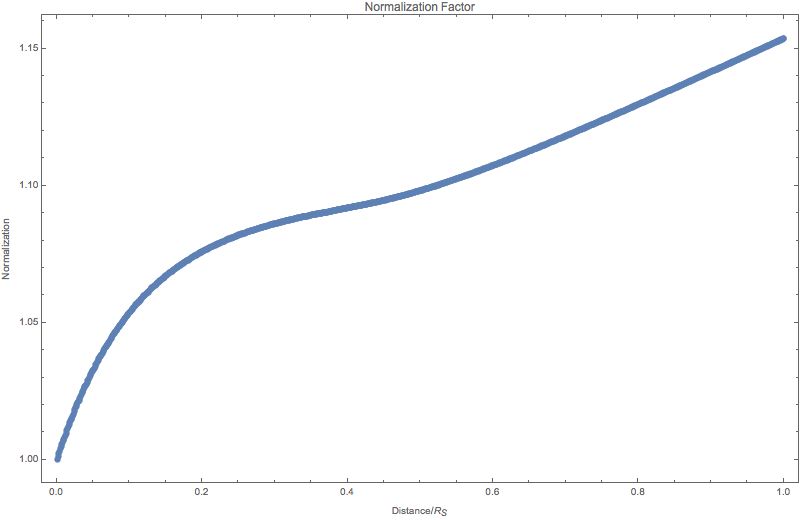
\includegraphics{numericalMSW3Flavor-normalization.png}
\caption{Normalization factor as a function of distance.}\end{figure}
\begin{figure}[htbp]
\centering
\capstart

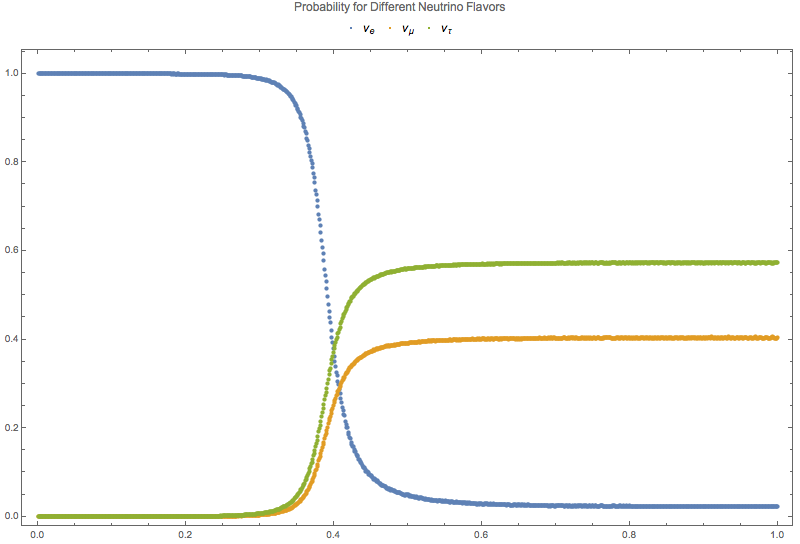
\includegraphics{numericalMSW3Flavor-probabilities.png}
\caption{Probability for each flavor of neutrinos.}\end{figure}

Applying a number density function \(n(x) = 10^{-13 - 4.3 x}\) to the system, the small scale oscillations are revived,
\begin{figure}[htbp]
\centering
\capstart

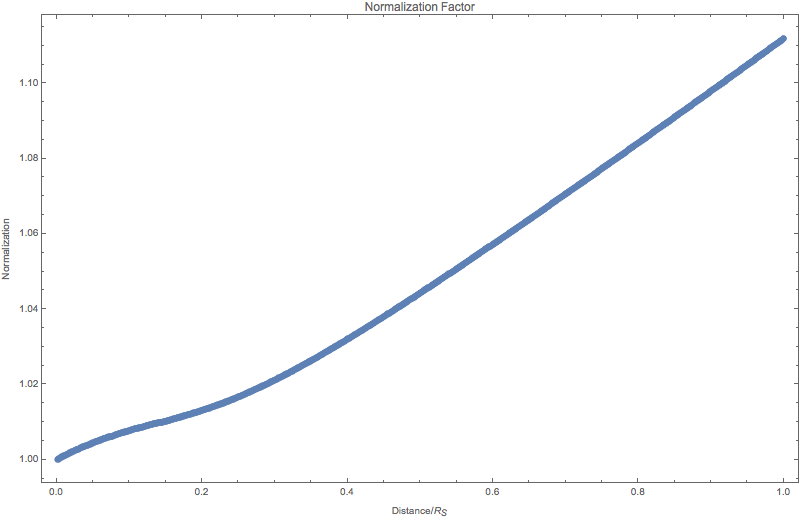
\includegraphics{numericalMSW3Flavor-2-norm.png}
\caption{Normalization of the states for numerical 3 flavor oscillation in the sun with density profile \(10^{-13 - 4.3 x}\).}\end{figure}
\begin{figure}[htbp]
\centering
\capstart

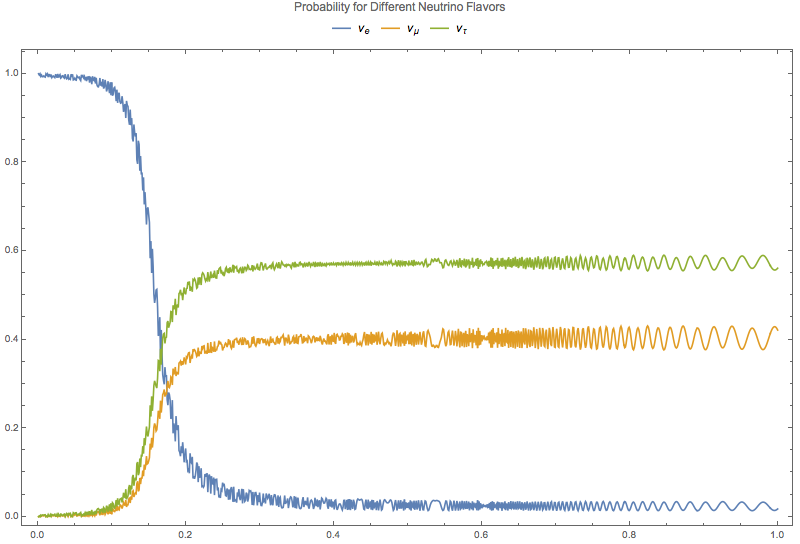
\includegraphics{numericalMSW3Flavor-2-probability.png}
\caption{Numerical results for 3 flavor oscillation in the sun with density profile \(10^{-13 - 4.3 x}\).}\end{figure}
\begin{figure}[htbp]
\centering
\capstart

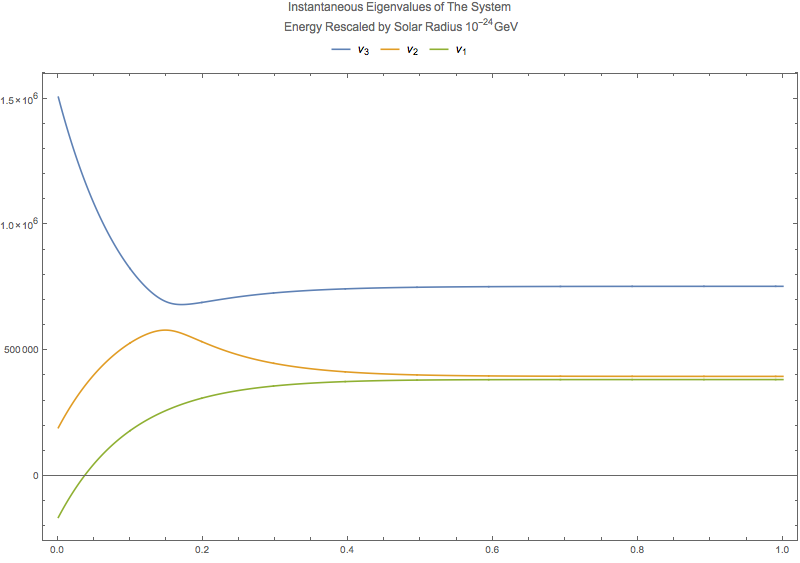
\includegraphics{numericalMSW3Flavor-minus13-Inst-Eigen-Energies.png}
\caption{Eigenenergies for density profile \(10^{-13 - 4.3 x}\).}\end{figure}
\begin{figure}[htbp]
\centering
\capstart

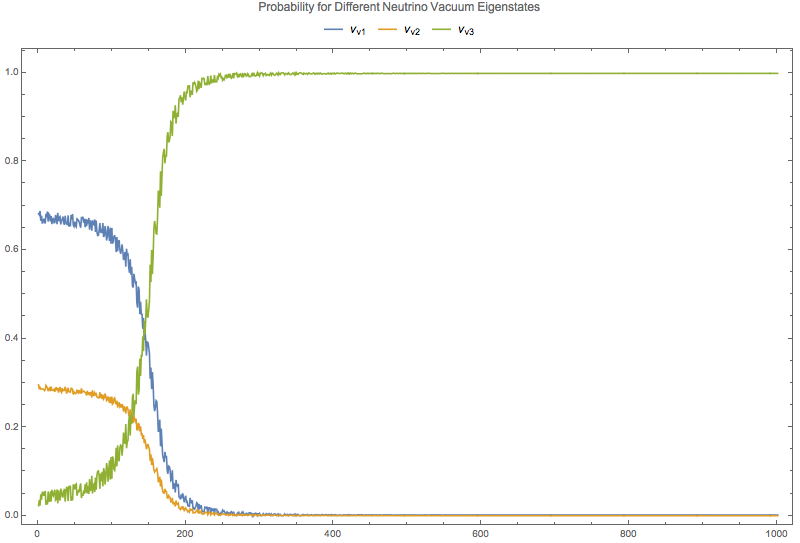
\includegraphics{numericalMSW3Flavor-vac-eigen-prob.png}
\caption{Survival probabilities for different vacuum mass eigenstates for 3 flavor oscillation in the sun with density profile \(10^{-13 - 4.3 x}\).}\end{figure}

An interesting notion is the survival probability for the instantaneous eigenstates.
\begin{figure}[htbp]
\centering
\capstart

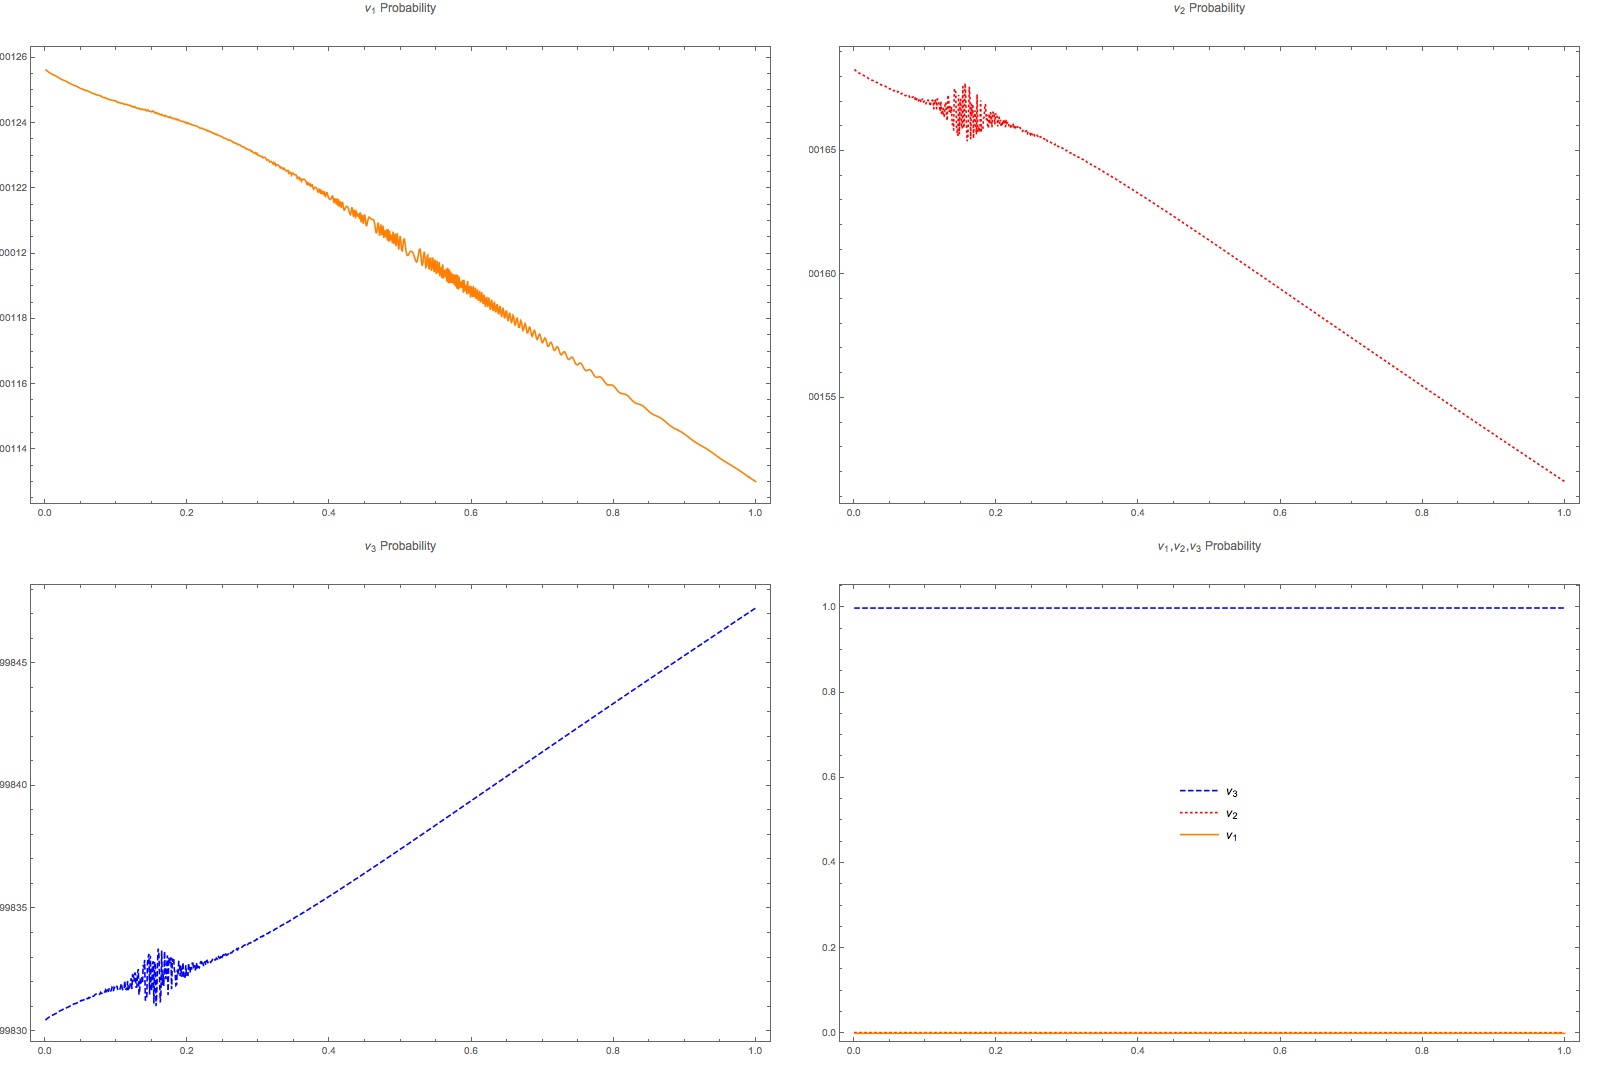
\includegraphics{instanEigenstetes-minus13-Grid.png}
\caption{Probability for the instantaneous eigenstates for matter profile \(10^{-13 - 4.3 x}\).}\end{figure}

Lower matter density will have less suppression on vacuum oscillations.
\begin{figure}[htbp]
\centering
\capstart

\includegraphics{numericalMSW3Flavor-minus14matter.png}
\caption{Numerical results for 3 flavor oscillation in the sun with density profile \(10^{-14 - 4.3 x}\).}\end{figure}


\subsection{Ternary Diagram}
\label{msw:ternary-diagram}
High matter density suppresses the vacuum oscillations which is clearly shown on a ternary diagram.
\begin{figure}[htbp]
\centering
\capstart

\includegraphics{mass-1.png}
\caption{Ternary diagram for MSW effect shows that the vacuum oscillations in this case is suppressed. Comparing this with the survival probability, the survival probability for electron neutrino drops to a value and the rapid oscillations start to show up. The drop is the movement in the ternary diagram from the right-bottom cornor to the tau neutrino axis. These rapid oscillations corresponds to the T-shaped tip at the other end of the line.}\end{figure}
\begin{figure}[htbp]
\centering
\capstart

\includegraphics{mass-1-scatter.png}
\caption{Ternary diagram for MSW effect with homogeneously descretized position \(x\) with matter profile \(10^{-13-4.3x}\mathrm{GeV^3}\). We can see clearly that the system stays on the two ends to the line for a longer time that in the middle where the transition happens very quickly. This can also be seen in the survival probability plot.}\end{figure}
\begin{figure}[htbp]
\centering
\capstart

\includegraphics{matter-inst-eigen-e-1.png}
\caption{Ternary diagram for instantaneous eigenstates with matter profile \(10^{-13-4.3x}\mathrm{GeV^3}\). The system starts from almost the second instantaneous state then moves along the state that \(\nu_1=0\).}\end{figure}
\begin{figure}[htbp]
\centering
\capstart

\includegraphics{matter-inverted-1.png}
\caption{Ternary diagram for MSW effect with inverted hierarchy \(\Delta m_{23} = m_3^2 - m_2^2<0\). The shape changes a lot since the frequencies changes a lot.}\end{figure}


\section{Refs and Notes}
\label{msw:refs-and-notes}\begin{enumerate}
\item {} 
Wolfenstein, L. (1978). Neutrino oscillations in matter. Physical Review D, 17(9), 2369–2374. doi:10.1103/PhysRevD.17.2369

\item {} 
Wolfenstein, L. (1979). Neutrino oscillations and stellar collapse. Physical Review D, 20(10), 2634–2635. doi:10.1103/PhysRevD.20.2634

\item {} 
Parke, S. J. (1986). Nonadiabatic Level Crossing in Resonant Neutrino Oscillations. Physical Review Letters, 57(10), 1275–1278. doi:10.1103/PhysRevLett.57.1275

\item {} 
Bethe, H. A. (1986). Possible Explanation of the Solar-Neutrino Puzzle. Physical Review Letters, 56(12), 1305–1308. doi:10.1103/PhysRevLett.56.1305

\end{enumerate}


\chapter{Parametric Resonance}
\label{parametric:parametric-resonance}\label{parametric::doc}
\index{Parametric Resonance}

\section{Parametric Resonance}
\label{parametric:index-0}\label{parametric:id1}

\subsection{Evolution Operator}
\label{parametric:evolution-operator}
For constant matter density, the state after a propagation of distance \(X\) is given by the evolution operator,
\begin{gather}
\begin{split}\Psi^{f}(x_0+X) = \mathscr{U}^{m} (X) \Psi^f(x_0),\end{split}\notag
\end{gather}
where \(\mathscr{U}^{m}\) is the evolution operator in flavor basis, which is obtained directly using
\begin{gather}
\begin{split}\mathscr{U}^m (x) = \exp\left(  -i H^f x \right),\end{split}\notag
\end{gather}
or from a rotation of evolution operator in matter basis.

The Hamiltonian in flavor basis is simply written in terms of Pauli matrices,
\begin{gather}
\begin{split}H^f = \frac{\omega}{2} \left( \sin 2\theta \sigma_1 + (\hat\lambda - \cos 2\theta) \sigma_3 \right),\end{split}\notag
\end{gather}
which, fortunately, can be simplified to a vector product of the Pauli matrices vector and another vector. To find out the other vector, we define
\begin{gather}
\begin{split}\vec \sigma = \left( \sigma_1, \sigma_2,\sigma_3 \right).\end{split}\notag
\end{gather}
Then we require
\begin{gather}
\begin{split}H^f \equiv \frac{\omega_m}{2} \vec n\cdot \vec \sigma .\end{split}\notag
\end{gather}
Compare this expression with the previous result for \(H^f\), we solve
\begin{gather}
\begin{split}\vec n = \frac{\omega}{\omega_m } \left( \sin 2\theta ,  0 , \hat\lambda  - \cos 2\theta  \right),\end{split}\notag
\end{gather}
where \(\vec n\) is indeed a unit vector.

Using this new simplified expression for Hamiltonian, we have
\begin{gather}
\begin{split}\mathscr{U}^m (x) &= \exp\left( -i H^f x \right) \\
& = \exp \left( - i \frac{\omega_m}{2} x \vec n\cdot \vec \sigma \right).\end{split}\notag
\end{gather}
\begin{notice}{note}{Euler's Formula for Pauli Matrices}
\begin{gather}
\begin{split}e^{i \phi \vec n \cdot \vec \sigma} = I \cos \phi + i \vec n \cdot \vec \sigma \sin \phi.\end{split}\notag
\end{gather}
To prove it, Taylor expansion of the exponential and anticommutation relations are needed.
\end{notice}

Using Euler's formula, we obtain the expanded form of the evolution operator,
\begin{gather}
\begin{split}\mathscr{U}^m (x) = I \cos \left( \frac{\omega_m}{2} x \right) - i \vec n \cdot \vec \sigma \sin \left( \frac{\omega_m}{2} x \right),\end{split}\notag
\end{gather}
where we can define a phase function for simplicity, :math:{\color{red}\bfseries{}{}`}phi(x) =  frac\{omega\_m\}\{2\} x {\color{red}\bfseries{}{}`}. The evolution becomes
\begin{gather}
\begin{split}\mathscr{U}^m (x) = I \cos \phi(x) - i \vec n \cdot \vec \sigma \sin \phi(x).\end{split}\notag
\end{gather}

\subsection{Two Slabs}
\label{parametric:two-slabs}
For two slabs with different matter potential right next to each other, the evolution operator for the two slabs is simply the multiplication of the two evolution operator for each slab,
\begin{gather}
\begin{split}\mathscr{U}^f (X_1+X_2) = \mathscr{U}^f(X_2)\mathscr{U}^f(X_1),\end{split}\notag
\end{gather}
where \(X_1\) and \(X_2\) are the thickness of the slabs.

Apply the formalism of Pauli matrices, we have
\begin{gather}
\begin{split}\mathscr{U}^f (X_1+X_2) &= \left( I \cos \phi(X_2) - i \vec n_2 \cdot \vec \sigma \sin \phi(X_2) \right)  \left( I \cos \phi(X_1) - i \vec n_1 \cdot \vec \sigma \sin \phi(X_1) \right) \\
& = \cos \phi(X_2)\cos \phi(X_1) - i\vec n _1 \cdot \vec \sigma \cos\phi(X_2) \sin \phi(X_1) - i \vec n_2 \cdot \vec \sigma \sin \phi(X_2) \cos \phi(X_1) - (\vec n_2 \cdot \vec \sigma)(\vec n_1 \cdot \vec \sigma) \sin \phi (X_2) \sin \phi(X_1).\end{split}\notag
\end{gather}
Notice that
\begin{gather}
\begin{split}&(\vec n_2 \cdot \vec \sigma)(\vec n_1 \cdot \vec \sigma)  \\
=& \frac{\omega}{\omega_{m1}}\frac{\omega}{\omega_{m2}}( \sin 2\theta \sigma_1 + ( \hat\lambda_{m2} - \cos 2\theta ) \sigma_3 )( \sin 2\theta \sigma_1 + (\hat\lambda_{m1} -\cos 2\theta ) \sigma_3 ) \\
=& \frac{\omega}{\omega_{m1}}\frac{\omega}{\omega_{m2}} ( \sin 2\theta \sin 2\theta + \cos 2\theta \cos 2\theta + \hat \lambda_{m1}\hat\lambda_{m2} - \hat\lambda_{m1} \cos 2\theta - \hat\lambda_{m2}\cos 2\theta - \sin 2\theta \sigma_1 (\hat\lambda_{m1}- \cos 2\theta) \sigma_3  -  (\hat\lambda_{m2}- \cos 2\theta) \sigma_3 \sin 2\theta \sigma_1 ) \\
=& \vec n_1 \cdot \vec n_2 + i \vec n_1 \times \vec n_2 \sigma_2.\end{split}\notag
\end{gather}
Thus the result for the evolution operator is
\begin{gather}
\begin{split}\mathscr{U}^f (X_1+X_2) & = \cos \phi(X_2)\cos \phi(X_1) - i\vec n _1 \cdot \vec \sigma \cos\phi(X_2) \sin \phi(X_1) - i \vec n_2 \cdot \vec \sigma \sin \phi(X_2) \cos \phi(X_1) - (\vec n_1 \cdot \vec n_2 + \vec n_1 \times \vec n_2) \sin \phi (X_2) \sin \phi(X_1) \\
& = \cos \phi(X_1) \cos \phi(X_2) - \sin \phi(X_1)\sin \phi(X_2) \vec n_1\cdot \vec n_2  - i \vec \sigma\cdot ( \sin \phi(X_1) \cos \phi(X_2) \vec n_1 + \cos \phi(X_1) \sin \phi(X_2) \vec n_2 -  \sin \phi (X_1) \sin \phi(X_2) \vec n_1 \times \vec n_2 )\\
& \equiv R - i \vec \sigma \cdot \vec I,\end{split}\notag
\end{gather}
where
\begin{gather}
\begin{split}R &= \cos \phi(X_1) \cos \phi(X_2) - \sin \phi(X_1)\sin \phi(X_2) \vec n_1\cdot \vec n_2 \\
\vec I & = \sin \phi(X_1) \cos \phi(X_2) \vec n_1 + \cos \phi(X_1) \sin \phi(X_2) \vec n_2 -  \sin \phi (X_1) \sin \phi(X_2) \vec n_1 \times \vec n_2.\end{split}\notag
\end{gather}
To carry out the calculation of multiple periods of such, it is easier to rewrite the evolution operator into exponential form. To do so we need to define
\begin{gather}
\begin{split}R & = \cos \Phi ,\\
\vec N & = \frac{\vec I}{\lvert \vec I \rvert},\\
\lvert \vec I \rvert & = \sin \Phi.\end{split}\notag
\end{gather}
Using these representations, we can easily apply Euler's formula backwards,
\begin{gather}
\begin{split}\mathscr{U}^f(X_1+X_2) = \exp \left( -i (\vec N \cdot  \vec \sigma) \Phi \right).\end{split}\notag
\end{gather}
For a lot of such potentials right next to each other, we have
\begin{gather}
\begin{split}\mathscr{U}^f(k(X_1+X_2)) = \exp \left( -i k (\vec N \cdot  \vec \sigma) \Phi \right).\end{split}\notag
\end{gather}
This is verified in Giunti's book.

Then we can calculate the transition probability, which is given in Giunti's book,
\begin{gather}
\begin{split}P_{\nu_e\to\nu_\mu} (k(X_1+X_2) ) = \left( 1 - \frac{I_3^2}{\lvert \vec I \rvert^2}  \right) \sin^2 k\Phi ,\end{split}\notag
\end{gather}
which gives us the resonance condition \(I_3=0\), i.e.,
\begin{gather}
\begin{split}\frac{\tan \phi(X_1)}{\tan \phi(X_2)} = -\frac{\cos 2\theta_{m2}}{\cos 2\theta_{m1}},\end{split}\notag
\end{gather}
with \(\phi(X_i)=\frac{\omega_{mi}}{2}X_i\).


\section{Refs and Notes}
\label{parametric:refs-and-notes}
I did some calculations based on Giunti's book so that I can really understand each step of the derivations.
\begin{enumerate}
\item {} 
Giunti, C., \& Kim, C. W. (2007). Fundamentals of Neutrino Physics and Astrophysics. Oxford University Press. doi:10.1093/acprof:oso/9780198508717.001.0001

\end{enumerate}


\chapter{Collective Behavior}
\label{collective:collective-behavior}\label{collective::doc}
In a dense neutrino environment, neutrino oscillations could exhibit collective behaviors or synchronized behaviors.

The key of such a behavior is the self interaction between neutrinos.

\begin{notice}{note}{Phonon}

In solid state physics, phonons are the collective behavior of atom or molecule oscillations. The necessary condition for such a behavior is the interaction between atoms or molecules.
\end{notice}

Backgrounds of collective effect:
\begin{enumerate}
\item {} 
Matter background

\item {} 
Neutrino background
a) sychronized oscillations: neutrino neutrino interaction potential is large compared toordinary oscillation frequencies in vacuum/medium + large asymmetry between neutrino and antineutrino distributions
b) bipolar oscillations: neutrino and antineutrino oscillate in opposite directions; non-zero vacuum mixing angle + some conditions of mass hierarchy. neutrino-neutrino interaction ( \(\mu=\sqrt{2}G_F n_\nu\) ) is larger than vacuum oscillatioin frequency \(\omega=\Delta m\) . like a torque applys to a top where instabilities happpen as the torque force is too big (top wobbles and flips).

\end{enumerate}

\begin{notice}{note}{Ref}
\begin{enumerate}
\item {} 
Raffelt, G. \& Smirnov, A. \href{http://journals.aps.org/prd/abstract/10.1103/PhysRevD.74.105010}{Self-induced spectral splits in supernova neutrino fluxes.} \emph{Phys. Rev. D} \textbf{76}, (2007). (This paper includes a very brief summary of sychronized and bipolar.)

\end{enumerate}
\end{notice}


\section{Collective Phenomenon}
\label{collective:collective-phenomenon}
Neutrino-neutrino interaction can be described by the following Feymann diagram.
\begin{figure}[htbp]
\centering
\capstart

\includegraphics{refractiveFey.png}
\caption{They just exchange their momenta.}\end{figure}

Electron neutrinos can exchange momentum with other neutrinos including itself. Suppose we have a muon neutrino moving forward, and vacuum oscillations,
\begin{figure}[htbp]
\centering
\capstart

\includegraphics{collectiveToyModel.png}
\caption{Toy model to illustrate the basics of collective behavior.}\end{figure}

At site 1, electron neutrino becomes muon neutrino after 1 oscillation length and moving top, while the muon neutrino coming from the left becomes electron neutrino. If they interact, their momenta will be exchanged, leaving a muon neutrino moving to the right and carrying the momentum of the neutrino moving up.

After the interaction at site 1, a electron neutrino is moving up and transforms to a muon neutrino at site 2. The interaction at site 1 will be repeated all the way along the trajectory. And we have all muon neutrinos coming out right of the sites which should be electron neutrinos if we only have vacuum oscillation.

This is a toy model of collective oscillation.

\index{Spectral Split}

\subsection{Spectral Split}
\label{collective:spectral-split}\label{collective:index-0}
A spectral split phenomenon has been observed in calculations. \footnote{
Duan, H., Fuller, G., Carlson, J. \& Qian, Y.-Z. \href{http://journals.aps.org/prd/abstract/10.1103/PhysRevD.74.105014}{Simulation of coherent nonlinear neutrino flavor transformation in the supernova environment: Correlated neutrino trajectories.} \emph{Phys. Rev. D} \textbf{74}, (2006).
}
\begin{figure}[htbp]
\centering
\capstart

\includegraphics{spectralSplit.png}
\caption{Spectral split due to neutrino self interaction. Total flavour content is not changed however the flavour exchange momentum which is refered to spectral split.}\end{figure}

\index{Bipolar Model}

\section{Bipolar Model}
\label{collective:bipolar-model}\label{collective:index-1}\begin{figure}[htbp]
\centering
\capstart

\includegraphics{bipolar.png}
\caption{Biplar}\end{figure}

The neutrinos are generated in two classes with the same number density thus making up two total flavour isospins. Neutrino-neutrino interaction could make the oscillation unstable if it is too large. \footnote{
Raffelt, G. \& Smirnov, A. \href{http://journals.aps.org/prd/abstract/10.1103/PhysRevD.74.105010}{Self-induced spectral splits in supernova neutrino fluxes.} \emph{Phys. Rev. D} \textbf{76}, (2007).
}

\index{Isotropic Neutrino Gas}

\section{Dense Homogeneous Isotropic Neutrino Gas}
\label{collective:dense-homogeneous-isotropic-neutrino-gas}\label{collective:index-2}
The total flavour isospin could precess around effective hamiltonian like the precession of gyroscope with all the indvidual flavour isospin precess around the total flavour isospin.


\section{Refs \& Notes}
\label{collective:refs-notes}
Some papers:
\begin{enumerate}
\item {} 
\href{http://link.aps.org/pdf/10.1103/PhysRevD.74.123004}{Collective neutrino flavor transformation in supernovae}

\end{enumerate}


\chapter{Qualitative Analysis}
\label{qualitative:qualitative-analysis}\label{qualitative::doc}

\section{Oscillation Period, Frequency and Energy}
\label{qualitative:oscillation-period-frequency-and-energy}
\textbf{The mixing angles plays an important role in the amplitude of the oscillations while the energy scales play a role in the periods.}

In vacuum, 2 flavor oscillations, only one energy scale that is important enough which gives us the oscillation period (oscillation length) and frequency,
\begin{gather}
\begin{split}\omega &= \frac{\Delta m^2}{2E},\\
l_v &= \frac{2\pi}{\omega} = \frac{4\pi E}{\Delta m^2}.\end{split}\notag
\end{gather}
\begin{notice}{note}{3 Flavor Energy Scales}

As long as we approach the 3 flavor oscillations, two mass square differences show up in the system thus giving us two energy scales, two periods and two frequencies. They are
\begin{gather}
\begin{split}\omega_{12} &= \frac{\Delta m_{12}^2}{2E} \\       l_{v12} & = \frac{2\pi}{\omega_{12}},\end{split}\notag
\end{gather}
and
\begin{gather}
\begin{split}\omega_{23} &= \frac{\Delta m_{23}^2}{2E} \\
l_{v23} & = \frac{2\pi}{\omega_{23}}.\end{split}\notag
\end{gather}\end{notice}

In matter, the interaction with matter \(\Delta \equiv \sqrt{2} G_F n\) in related to another oscillation length, which is
\begin{gather}
\begin{split}l_m = \frac{2\pi}{\Delta} = \frac{2\pi}{\sqrt{2}G_F n} .\end{split}\notag
\end{gather}
\begin{notice}{note}{Importance of Oscillation Period}

The oscillation length and frequency in fact is related to the energy scales. As the energy scales match each other, interesting things could happen. In the case of neutrinos, MSW resonance can happen.
\end{notice}

\begin{notice}{note}{Fermi Constant}

Fermi constant is \(G_F=1.17\times 10^{-5}\mathrm{GeV^{-2}}\). The conversion between distance and energy is given by \(1\mathrm{fm}\cdot 197\mathrm{MeV}=1\).
\end{notice}

With the definition of these oscillation lengths, a comparison between them can be made. Choose \(\Delta m_{21}^2=10^{-4}\times 10^{-18}\mathrm{GeV^{2}}\), we have
\begin{gather}
\begin{split}l_v &= 4\times 10^{19}\pi \left( \frac{E}{1 \mathrm{MeV} } \right) \mathrm{GeV^{-1}} = 7.9\times 10^3 \pi   \left( \frac{E}{1 \mathrm{MeV} } \right)\mathrm{m}  \\
l_m &=  1.2\times 10^{19}\pi \left( \frac{10^{-14}}{n} \right) \mathrm{GeV^{-1}} = 1.2\times 10^4\pi \left( \frac{10^{-24}\mathrm{cm^{-3}}}{n} \right) .\end{split}\notag
\end{gather}
There are relations between energy of neutrinos and the number density of electrons when the two lengths are equal.
\begin{figure}[htbp]
\centering
\capstart

\includegraphics{comparisonVacOscLengthMatterLength.png}
\caption{Comparison of the lengths. The two length are equal if}{\small \begin{gather}
\begin{split}\left(\frac{10^{-14}}{n} \right) = 3.3 \left( \frac{E}{10^{-3}}\right),\end{split}\notag
\end{gather}
in which \(n\) is in \(\mathrm{GeV^3}\) while \(E\) is in unit of \(\mathrm{GeV}\).
}\end{figure}

On the other hand, the overall oscillation length in matter is
\begin{gather}
\begin{split}l &= \frac{2\pi}{\omega_m} \\
& = \frac{2\pi}{\omega \sqrt{ \hat\Delta^2 + 1 - 2 \hat\Delta \cos 2\theta_v }} \\
& = \frac{l_v}{ \sqrt{\left(\frac{l_v}{l_m} \right)^2 +1 - 2\frac{l_v}{l_m}\cos 2\theta_v  }} .\end{split}\notag
\end{gather}
This expression shows exactly why the different length scales are important.
\begin{enumerate}
\item {} 
\(\lvert \frac{l_v}{l_m} \rvert \ll 1 \Rightarrow l\to l_v\), matter effect is minimal.

\item {} 
\(\lvert \frac{l_v}{l_m} \rvert \gg 1 \Rightarrow l\to 0\), matter effect kills the oscillations.

\item {} 
\(\lvert \frac{l_v}{l_m}\rvert \sim 1 \Rightarrow l\to \frac{l_v}{2\sin\theta_v}\), more interesting region, assuming \(\sin\theta_v>0\). To linear approximation,
\begin{gather}
\begin{split}l \approx \frac{l_v}{2\sin\theta_v} \left( 1 -  \frac{l_v/l_m - 1}{2} \right) = \frac{l_v}{4\sin\theta_v} \left( 1 -  \frac{l_v}{l_m } \right) .\end{split}\notag
\end{gather}
notice that at resonance
\begin{gather}
\begin{split}l = \frac{l_v}{2\sin \theta_v}.\end{split}\notag
\end{gather}
\end{enumerate}

Another important thing about these lengths is that \(l_v\) is a function of energy which is that higher energy means longer oscillation length as shown in figure on comparison of vacuum oscillation length with matter length. This is important because we can always find the a energy that is at resonance with the matter density, as long as the energy still makes sure the neutrinos are relativistic. So a spectral swap is possible.


\section{Refs and Notes}
\label{qualitative:refs-and-notes}\begin{enumerate}
\item {} 
Wolfenstein, L. (1979). Neutrino oscillations and stellar collapse. Physical Review D, 20(10), 2634–2635. doi:10.1103/PhysRevD.20.2634

\end{enumerate}


\chapter{Instability}
\label{instability:instability}\label{instability::doc}
Instability of neutrino oscillation means the rapid growth of the oscillations.

\begin{notice}{note}{Question}

Where do we get the perturbations?
\end{notice}

\begin{notice}{note}{Answer}

TBD.
\end{notice}

\index{Linear Stability Analysis}

\section{Linear Stability Analysis}
\label{instability:index-0}\label{instability:linear-stability-analysis}
\index{Bimodal Instability}

\section{Bimodal Instability}
\label{instability:bimodal-instability}\label{instability:index-1}
An example of such intability happens in a system composed of equal amounts of neutrinos and antineutrinos. Flavour transform occurs due to
\begin{gather}
\begin{split}\nu_e + \bar{\nu_e} \leftrightarrow \nu_x + \bar{\nu_x}.\end{split}\notag
\end{gather}
Vacuum mixing angle triggers the flavour instability.

Neutrino oscillatioins are synchronized but with a small amplitude inside a SN core (suppressed by matter effects), \footnote{
Wolfenstein, L. \href{http://journals.aps.org/prd/abstract/10.1103/PhysRevD.17.2369}{Neutrino oscillations in matter.} \emph{Phys. Rev. D} \textbf{17}, 23692374 (1978). Or check papers of MSW effect such as Wick Haxton's excellent review.
} which basically pin down the flavour transformation. As the flux reaches

\index{Multi-angle Instability}

\section{Multi-angle Instability}
\label{instability:index-2}\label{instability:multi-angle-instability}
Non-isotropic neutrino gas would have velocity (or momentum) related interactions, \(1-\vec v_p\cdot\vec v_q\), which is in fact a \(1 -\frac{2\sqrt{\pi}}{\sqrt{3}} Y_1^0(\theta,\phi)\) term.

A small anisotropy leads to a runaway flavor equipartition. \footnote{
Raffelt, G. \& Smirnov, A. \href{http://journals.aps.org/prd/abstract/10.1103/PhysRevD.75.083002}{Self-induced spectral splits in supernova neutrino fluxes.} \emph{Phys. Rev. D} \textbf{76}, (2007). In this paper the author adds a small perturbation to a perfectly isotropic neutrino antineutrino gas. The results show multi-angle instability.
}
\begin{figure}[htbp]
\centering
\capstart

\includegraphics{multiangleInstability.png}
\caption{A figure from Raffelt \& Simirnov (2007) shows the instability from anisotropic small perturbations. Potential energy grows expotentially, where \(-E_1 = \mu/4 \vec{D_1}^2\) .}\end{figure}


\section{MAA}
\label{instability:maa}\begin{figure}[htbp]
\centering
\capstart

\includegraphics{sphericalAngles.png}
\caption{A sphere on wikipedia \href{https://commons.wikimedia.org/wiki/File:Azimuth-Altitude\_schematic.svg}{File:Azimuth-Altitude schematic.svg}}\end{figure}

Multi-azimuth angle (MAA) instability, first discovered by Georg Raffelt et al, in the work \href{http://journals.aps.org/prl/abstract/10.1103/PhysRevLett.111.091101}{Axial Symmetry Breaking in Self-Induced Flavor Conversion of Supernova Neutrino Fluxes} , \footnote{
Raffelt, G., Sarikas, S. \& Seixas, D. \emph{Axial Symmetry Breaking in Self-Induced Flavor Conversionof Supernova Neutrino Fluxes. \textless{}http://journals.aps.org/prl/abstract/10.1103/PhysRevLett.111.091101\textgreater{}} \emph{Phys. Rev. Lett.} \textbf{111}, (2013).
} is an intrinsic symmetry breaking. The point is to allow angle modes to evolve independently.

This instability may come from the term that is related to the velocity of neutrinos in the Hamiltonian.

This could happen even for a perfectly symmetric emission.


\section{Neutrino Self Interaction and Instability}
\label{instability:neutrino-self-interaction-and-instability}

\section{Refs \& Notes}
\label{instability:refs-notes}
.


\chapter{Pictures}
\label{picture:pictures}\label{picture::doc}
There are several pictures to visualize the oscillations of neutrinos.


\section{Magnetic Spin}
\label{picture:magnetic-spin}\begin{figure}[htbp]
\centering
\capstart

\includegraphics{larmor.png}
\caption{Image source: \href{http://hyperphysics.phy-astr.gsu.edu/hbase/magnetic/larmor.html}{Larmor Precession} .}\end{figure}

Recall that torque of a magnetic spin in a magnetic field is calculated as
\begin{gather}
\begin{split}\vec \tau = \vec \mu \times \vec B,\end{split}\notag
\end{gather}
while torque is by definition \(\vec \tau = \frac{d}{dt}\vec L\). So we have, for such a system, the equation of motion is
\begin{gather}
\begin{split}\frac{d}{dt}\vec L = \vec \mu \times \vec B.\end{split}\notag
\end{gather}
In the case of electron quantum magnetic spin, \(\vec \mu\) is proportional to the angular momentum \(\vec L\), i.e., \(\vec \mu = \frac{-e}{2m_e}\vec L\propto \vec L\).

So the equation of motion becomes
\begin{gather}
\begin{split}\frac{d}{dt}\vec L \propto \vec L \times \vec B.\end{split}\notag
\end{gather}
\begin{notice}{note}{Equation of Motion for Neutrino Flavor Polarization Vector}

That EoM is
\begin{gather}
\begin{split}\frac{d}{dt} \vec P_\omega = (\omega \vec B + \lambda \vec L + \mu \vec D)\times \vec P_\omega ,\end{split}\notag
\end{gather}
where the quantities can be found in Duan, H., Fuller, G. \& Qian, Y.-Z. Collective Neutrino Oscillations. \emph{Annu. Rev. Nucl. Part. Sci.} \textbf{60}, 569–594 (2010).

Now it is clear that the two system has very similar EoM.
\end{notice}


\section{Neutrino Flavour Isospin}
\label{picture:neutrino-flavour-isospin}
Neutrino flavour isospin \footnote{
\href{http://journals.aps.org/prd/abstract/10.1103/PhysRevD.74.123004}{Collective neutrino flavor transformation in supernovae}
}
\begin{gather}
\begin{split}\mathbf s = \psi^{f\dagger} \frac{\mathbf\sigma}{2} \psi^f,\end{split}\notag
\end{gather}
where
\begin{gather}
\begin{split}\psi^f_\nu & = \begin{pmatrix} a_{\nu_e} \\ a_{\nu_x} \end{pmatrix} \\
\psi^f_{\bar \nu} & = \begin{pmatrix} - a_{\bar\nu_x} \\ a_{\bar\nu_e} \end{pmatrix}\end{split}\notag
\end{gather}
The equation of motion for isospin is
\begin{gather}
\begin{split}\frac{d}{dt}\mathbf s = \mathbf s \times \mathbf {H^{eff}}.\end{split}\notag
\end{gather}
Previously we have already seen the equations for a spinning top,
\begin{gather}
\begin{split}\frac{d}{dt}\vec S  =  \frac{\partial}{\partial t} \vec S  - \vec S \times \vec \Omega,\end{split}\notag
\end{gather}
where \(\vec\Omega = \vec n \dot\phi\). Consider conservation of momentum, we have
\begin{gather}
\begin{split}\frac{\partial}{\partial t} \vec S  = \vec S \times \vec \Omega,\end{split}\notag
\end{gather}
which is similar to the neutrino isospin equation of motion. \(\vec \Omega\) corresponds to \(\mathbf {H^{eff}}\).


\section{Coupled Pendulum}
\label{picture:coupled-pendulum}\begin{figure}[htbp]
\centering

\includegraphics{coupledPendulum.png}
\end{figure}

The equation of motion is
\begin{gather}
\begin{split}\begin{pmatrix}-\frac{d^2}{dt^2} - \left(\frac{g}{l}+\frac{k}{m}\right) & \frac{k}{m} \\ \frac{k}{m} & -\frac{d^2}{dt^2} - \left(\frac{g}{l}+\frac{k}{m}\right)\end{pmatrix} \begin{pmatrix} x \\ y \end{pmatrix} = \begin{pmatrix} 0 \\ 0 \end{pmatrix}\end{split}\notag
\end{gather}
Using Fourier transform, we will get the solutions,
\begin{gather}
\begin{split}\begin{pmatrix} x \\ y \end{pmatrix} = \begin{pmatrix}1 \\ 1 \end{pmatrix}A_1 \cos(\omega_1 t + \phi_1) + \begin{pmatrix}1 \\ -1\end{pmatrix} A_2 \cos (\omega_2 t + \phi_2)\end{split}\notag
\end{gather}
Recall that the state of neutrino after time \(t\) is
\begin{gather}
\begin{split}\ket{\psi(t)} = A_1 \ket{\nu_1} e^{-i E_1 t} + A_2 \ket{\nu_2} e^{- i E_2 t},\end{split}\notag
\end{gather}
where \(A_1\) and \(A_2\) are determined by initial condition. The real part of this, is exactly the same as the solution to coupled pendulum, where the physics is the transfer from one eigenstate to another.


\section{Gyroscope or Spinning Top Picture}
\label{picture:gyroscope-or-spinning-top-picture}

\subsection{A Classical Top}
\label{picture:a-classical-top}
The key concept of a classical gyroscope is the balance between gravity and angular momentum conservation, i.e., angular conservation in specific directions.

Angular momentum for a 3D rigid body with a axial symmetry in a \(\dot {\vec I}=0\) frame is
\begin{gather}
\begin{split}\vec S \to \begin{pmatrix} I_0 \omega_x \\ I_0 \omega_y \\ I\omega_z \end{pmatrix}\end{split}\notag
\end{gather}
The gyroscope should obey Euler's equations with extra Coriolis terms since we have decided to work in a rotation frame (\(\dot{\vec I}=0\)), \footnote{
Read Carl's lecture notes of \emph{Classical Mechanics} for this derivation.
}
\begin{gather}
\begin{split}M_x &= I_0 (\ddot \theta - \dot \phi^2\sin\theta \cos\theta) + I \dot \phi \sin\theta (\dot\phi\cos\theta + \dot \psi) \\
M_y & =  I_0 (\ddot \phi \sin\theta + 2 \dot \phi \dot\theta \cos\theta) - I \dot \theta (\dot \phi \cos\theta + \dot \psi) \\
M_z & = I (\ddot \psi + \ddot \phi \cos\theta - \dot\phi \dot \theta \sin\theta)\end{split}\notag
\end{gather}
with the torque for a top being
\begin{gather}
\begin{split}M_x & = m g z_G \sin\theta \\
M_y & = 0 \\
M_z & = 0 .\end{split}\notag
\end{gather}
\begin{notice}{note}{Note:}
\(\dot \psi\) is the spin of the top itself. More generally, the Euler equation is
\begin{gather}
\begin{split}\mathbf{I} \cdot \dot{\boldsymbol\omega} + \boldsymbol\omega \times \left( \mathbf{I} \cdot \boldsymbol\omega \right) = \mathbf{M}.\end{split}\notag
\end{gather}\end{notice}


\subsubsection{Steady Precession}
\label{picture:steady-precession}
A steady precession maintains the angle \(\theta\).
\begin{figure}[htbp]
\centering

\includegraphics{gyroscopeSteadyPrecession.png}
\end{figure}

Now we have \(\dot \theta =0\) so the Euler's equations reduces to,
\begin{gather}
\begin{split}\dot \phi  (I (\dot \phi \cos\theta +\dot \psi) - I_0\dot\phi \cos\theta) = M_x \equiv mg z_G\end{split}\notag
\end{gather}
For a steady state usually we can use this approximation \(\dot \psi \gg \dot\phi\).
\begin{gather}
\begin{split}\dot\phi = \frac{m g z_G }{I\dot\psi} .\end{split}\notag
\end{gather}
Now define \(\Omega  = \dot \phi\) and \(\omega = \dot \psi\). Our approximation becomes \(\omega \gg \Omega\).


\subsubsection{Unsteady Precession}
\label{picture:unsteady-precession}\begin{figure}[htbp]
\centering

\includegraphics{spinningTop.png}
\end{figure}


\section{Polarization Vector}
\label{picture:polarization-vector}
Polarization (for a two state system) is the difference of the probabilities of finding the system in the two difference normal states (spin up and spin down for example).


\subsection{Density Matrix}
\label{picture:density-matrix}
For a two-state system, an example of density matrix is
\begin{gather}
\begin{split}\hat \rho = W_1 \ket{\psi_a}\bra{\psi_a} + W_2 \ket{\psi_b}\bra{\psi_b}.\end{split}\notag
\end{gather}
When \(\{ \ket{\psi_a}, \ket{\psi_b} \}\) basis is chosen, density matrix can be written as a matrix,
\begin{gather}
\begin{split}\mathbf \rho = \begin{pmatrix} W_1 & 0 \\ 0 & W_2 \end{pmatrix},\end{split}\notag
\end{gather}
in which the two constants are the probability to find the system in each states respectively and they are called the population.

Rewrite the density matrix with Pauli matrices and identity,
\begin{gather}
\begin{split}\mathbf \rho = \frac{1}{2} ( \mathbf I + \vec{\mathbf \sigma} \vec P ).\end{split}\notag
\end{gather}
\begin{notice}{note}{Note:}
The reason we have a \(\frac{1}{2}\) is that by definition polarization vector is
\begin{gather}
\begin{split}\mathbf \rho &= a_0 \mathbf I + \mathbf {\sigma_x} a_x +  \mathbf {\sigma_y} a_y +  \mathbf {\sigma_z} a_z \\
& = a_0 \mathbf I + \vec a \vec{\mathbf \sigma}.\end{split}\notag
\end{gather}
However, trace of density matrix should be 1, which means \(\mathrm{Tr} \mathbf \rho = a_0 2 =1\) and we can find \(a_0=\frac{1}{2}\) noting that \(\mathrm {Tr}\mathbf \sigma_i = 0\).
\end{notice}

The important fact is that the values of polarization depends on the choice of basis.

More physical meanings can be obtained by chosing a good basis so that the density matrix is diagonalised by expressing it with components of polarization. \footnote{
Read quantum statistics book if more is needed.
}

Polarization, as the name indicates, should equal to
\begin{gather}
\begin{split}P = W_1 - W_2\end{split}\notag
\end{gather}
when it is aligned with z direction of Pauli matrices. Polarization vector is not a vector in real space but a vector of an imagined space.

\begin{notice}{note}{Take Out The Components}

How to project out the components of polarization vector? By multiplying on both sides the Pauli matrices.

Note that for Pauli matrices
\begin{gather}
\begin{split}\sigma_i \sigma_j = \epsilon_{ijk}\sigma_k + \delta_{ij}\mathbf I.\end{split}\notag
\end{gather}
Multiplying by \(\sigma_j\) on both sides of \(\rho =  \frac 1 2(\mathbf I+\vec P \cdot\vec \sigma)\), we get
\begin{gather}
\begin{split}\rho \sigma_j  = \frac 1 2(\mathbf I+\vec P \cdot\vec \sigma)\sigma_k.\end{split}\notag
\end{gather}
Apply the sigma algebra we discussed there, the result of this is
\begin{gather}
\begin{split}\rho \sigma_j = \frac{1}{2}(\sigma_k + P_i \sigma_i \sigma_j) \\
2 \rho \sigma_j - \sigma_k &= P_i (\epsilon_{ijk}\sigma_k + \delta_{ij}\mathbf I)\end{split}\notag
\end{gather}
We know that the trace of any Pauli matrix is zero. Take the trace of the equation,
\begin{gather}
\begin{split}\mathrm{Tr}\sigma_j =  P_j.\end{split}\notag
\end{gather}
All done.
\end{notice}


\section{Neutrino-neutrino Interaction and BCS Theory}
\label{picture:neutrino-neutrino-interaction-and-bcs-theory}
\begin{notice}{note}{BCS}

BCS Hamiltonian is
\begin{gather}
\begin{split}\hat H_{BCS} = \sum_k 2 \epsilon_k \hat t_k^0- \lvert G\rvert \hat T^\dagger \hat T\end{split}\notag
\end{gather}\end{notice}

Neutrino self interaction Hamiltonian is
\begin{gather}
\begin{split}\hat H = \sum_p \frac{\delta^2m}{2p}\hat B\cdot \vec J_\rho | \frac{\sqrt{2}G_F}{V}\vec J\cdot \vec J.\end{split}\notag
\end{gather}

\chapter{Models}
\label{models:models}\label{models::doc}

\section{Homogeneous and Isotropic Neutrino Gas}
\label{models:homogeneous-and-isotropic-neutrino-gas}
\(\vec P_\omega\) can be time-independent.

Regarding the discussion in Pictures, we know immediately that \(\vec H\) is aligned or anti-aligned with \(\vec P_\omega\) since
\begin{gather}
\begin{split}\vec H \times \vec P_\omega = 0,\end{split}\notag
\end{gather}
as \(\vec P_\omega\) is time-independent.

Anyway the equation we need to solve is then
\begin{gather}
\begin{split}\vec a\end{split}\notag
\end{gather}

\subsection{What to expect?}
\label{models:what-to-expect}
Without solving the equation, we know that


\subsection{Solving Eqns}
\label{models:solving-eqns}
\begin{notice}{note}{What is special in this model?}

To be added.
\end{notice}


\chapter{Neutrino Oscillation And Master Equation}
\label{mastereqn:neutrino-oscillation-and-master-equation}\label{mastereqn::doc}
\begin{notice}{note}{Question}

Why do we think about master equation?
\end{notice}

\begin{notice}{note}{Answer}

The terms we care the most are the populations of the states. One of the treatment of quantum master equation is to write down the closed equations for population terms only. A very beautiful example is the projection method invented by Zwawzig and Nakajiwa.
\end{notice}

\begin{notice}{note}{WHY}

Why do you need a master equation approach? IDK.
\end{notice}

\index{Quantum Master Equation}

\section{Quantum Master Equation}
\label{mastereqn:quantum-master-equation}\label{mastereqn:index-0}
\begin{notice}{note}{Projection Technique}

First of all define a diagonalizing operator \(\hat D\) which just keeps the diagonal elements and simply drops the off diagonal elements. We see that \(1-\hat D\) will eliminate all diagonal elements.

We can define the diagonalized density matrix as \(\hat \rho_d = \hat D \hat \rho\) and off-diagonalized density matrix as \(\hat \rho_{od} = (1-\hat D)\hat \rho\). As an application,
\begin{gather}
\begin{split}\hat \rho = \hat \rho_d + \hat \rho_{od} .\end{split}\notag
\end{gather}
Starting from the von Neumann equation,
\begin{gather}
\begin{split}i\hbar \partial_t \hat \rho = \left[\hat H, \hat \rho \right] .\end{split}\notag
\end{gather}
By using the Liouville operator,
\begin{gather}
\begin{split}\partial_t \hat \rho = -i \hat L \hat \rho .\end{split}\notag
\end{gather}
Apply \(\hat D\) and \(1-\hat D\) to the von Neumann equation,
\begin{gather}
\begin{split}\partial_t \hat \rho_d & = -i \hat D  \hat L \hat \rho \\
\partial_t \hat \rho _{od} & = -i (1 - \hat D)  \hat L \hat \rho .\end{split}\notag
\end{gather}
Use the relation that \(\hat \rho = \hat \rho_d + \hat \rho_{od}\), we have
\begin{gather}
\begin{split}\partial_t \hat \rho_d & = -i \hat D  \hat L \hat \rho_d - i \hat D  \hat L \hat \rho _ {od} \\
\partial_t \hat \rho _{od} & = - i (1 - \hat D)  \hat L \hat \rho _ d - i (1 - \hat D)  \hat L \hat \rho_{od}  .\end{split}\notag
\end{gather}
Solve the second equation using Green function technique,
\begin{gather}
\begin{split}\hat \rho_{od} = e^{-i(1-\hat D)\hat L t} + \int_0^t dt' e^{-i(1-\hat D) \hat L (t-t')}(-i(1-\hat D)\hat L \hat \rho_d(t')) .\end{split}\notag
\end{gather}
\begin{notice}{hint}{Hint:}
Recall that the solution for
\begin{gather}
\begin{split}\dot y + \alpha y = f\end{split}\notag
\end{gather}
is
\begin{gather}
\begin{split}y = e^{-\alpha t} y(0) + \int_0^t dt' e^{-\alpha (t-t')} f(t') .\end{split}\notag
\end{gather}\end{notice}

Insert this solution to the equation of \(\hat \rho_d\),
\begin{gather}
\begin{split}{\color{red}\partial_t \hat \rho_d = - i\hat D\hat L \hat \rho_d -  \hat D\hat L \int_0^t dt' e^{-i(1-\hat D) \hat L (t-t')}(1-\hat D)\hat L \hat \rho_d(t')} {\color{blue} - i \hat D \hat L e^{-i(1-\hat D)\hat L t} \rho_{od}(0) }.\end{split}\notag
\end{gather}
What happened to the blue term? It disapears when we apply the initial random phase condition.

When it happens we get our closed master equation for \(\hat \rho_d\), which is an equation for the probability.
\end{notice}

In our case of neutrinos, random phase condition is not really needed since we usually deal with the situation that electron neutrinos are appearant only.

In details, we have such a density matrix,
\begin{gather}
\begin{split}\mathbf\rho = \begin{pmatrix}\rho_{aa} &\rho_{ab} \\ \rho_{ba} & \rho_{bb}\end{pmatrix} .\end{split}\notag
\end{gather}
The quantum master equation we would like to use is
\begin{gather}
\begin{split}\partial_t \hat \rho_d = - i\hat D\hat L \hat \rho_d -  \hat D\hat L \int_0^t dt' e^{-i(1-\hat D) \hat L (t-t')}(1-\hat D)\hat L \hat \rho_d(t') .\end{split}\notag
\end{gather}

\section{Vacuum Oscillation Master Equation}
\label{mastereqn:vacuum-oscillation-master-equation}
Using this projection method, one can find out the master equation for vacuum oscillations.

\begin{notice}{note}{Pauli Matrices}

We will use Pauli matrices in the following part. Here is a review of them.
\begin{enumerate}
\item {} 
Pauli Matrices,
\begin{quote}
\begin{gather}
\begin{split}\sigma_1 &= \begin{pmatrix} 0 & 1 \\ 1 & 0 \end{pmatrix} \\
\sigma_2 & = \begin{pmatrix} 0 & -i \\ i & 0 \end{pmatrix} \\
\sigma_3 & = \begin{pmatrix} 1 & 0 \\ 0 & -1 \end{pmatrix}.\end{split}\notag
\end{gather}\end{quote}

\end{enumerate}
\begin{enumerate}
\setcounter{enumi}{1}
\item {} 
Commutation Relations,
\begin{quote}
\begin{gather}
\begin{split}[\sigma_1,\sigma_2] &= 2i \sigma_3 \\
[\sigma_2,\sigma_3] &= 2i \sigma_1 \\
[\sigma_3,\sigma_1] &= 2i \sigma_2.\end{split}\notag
\end{gather}
The general form is
\begin{gather}
\begin{split}[\sigma_i,\sigma_j] &= 2i \epsilon_{ijk} \sigma_k.\end{split}\notag
\end{gather}\end{quote}

\end{enumerate}
\end{notice}

All the Pauli matrices plus identity form a complate basis for 2 by 2 matrices. Vacuum oscillation Hamiltonian is
\begin{gather}
\begin{split}\mathbf H &\to \frac{\delta^2m}{4E} \begin{pmatrix} -\cos 2\theta & \sin 2 \theta \\ \sin 2\theta & \cos 2\theta \end{pmatrix} \\
& \equiv \begin{pmatrix} -c & s \\ s & c \end{pmatrix}\\
& = -c \begin{pmatrix} 1 & 0 \\ 0 & -1 \end{pmatrix} + s\begin{pmatrix} 0 & 1 \\ 1 & 0 \end{pmatrix} \\
& = -c \mathbf{\sigma_3} + s \mathbf{ \sigma_1},\end{split}\notag
\end{gather}
where \(c\equiv \frac{\delta^2 m}{4E}\cos 2 \theta\) and similarly for s.

\begin{notice}{note}{Liouville Operator}

Liouville operator in quantum mechanics is
\begin{gather}
\begin{split}\hat L  =  [H, *],\end{split}\notag
\end{gather}
where the asterisk is the slot for an operator.

In the case of vacuum oscillation, we can calculate the following results,
\begin{gather}
\begin{split}\hat L \sigma_1 &= [H, \sigma_1] = -2ic\sigma_2 \\
\hat L \sigma_2 &= [H, \sigma_2] = 2ic\sigma_1 + 2is\sigma_3.\end{split}\notag
\end{gather}
Notice that \(\sigma_3\) has diagonal terms only. It will dispear when we apply \(1-\mathscr D\) which removes the diagonal elements, i.e.,
\begin{gather}
\begin{split}(1-\mathscr D)\hat L \sigma_1 &= -2ic\sigma_2 \\
(1-\mathscr D)\hat L \sigma_2 &= 2ic\sigma_1.\end{split}\notag
\end{gather}
\textbf{Diagonalized density matrix} \(\rho_d=\mathrm {diag}(\rho_1,\rho_2)\) is
\begin{gather}
\begin{split}\mathrm {\rho_d} &= \begin{pmatrix} \rho_1 & 0 \\ 0 & \rho_2 \end{pmatrix} \\
& = \frac{1}{2} \left(\begin{pmatrix} \rho_1 -\rho_2 & 0 \\ 0 & \rho_2 -\rho_1 \end{pmatrix} + \begin{pmatrix} \rho_1+\rho_2 & 0 \\ 0 & \rho_1 + \rho_2 \end{pmatrix} \right) \\
& = \frac{1}{2}\left( (\rho_1-\rho_2)\sigma_3 + (\rho_1+\rho_2)\mathbf I \right)\end{split}\notag
\end{gather}
\begin{notice}{note}{Note:}
Actually \(\rho_1+\rho_2=1\) for such a system. We'll see the proof of this later.
\end{notice}

Apply \((1-\mathscr D)\hat L\) we get
\begin{gather}
\begin{split}(1-\mathscr D)\hat L \rho_d &= i s (\rho_2-\rho_1) \sigma_2,\\
\mathscr D \hat L \rho_d & = -\frac{1}{2}c (\rho_1+\rho_2)\sigma_3.\end{split}\notag
\end{gather}\end{notice}

\begin{notice}{note}{Exponential Operator}

Exponential operator is understood when series expansion is done,
\begin{gather}
\begin{split}e^{\hat A} = \hat I + \hat A + \frac{1}{2!}{\hat A}^2 + \frac{1}{3!} {\hat A}^3 +\cdots\end{split}\notag
\end{gather}\end{notice}

Recall that the master equation is
\begin{gather}
\begin{split}\partial_t \rho_d(t) &= - i \mathscr D \hat L \rho_d - \mathscr D\hat L \int_0^t dt' e^{-i(1-\mathscr D)\hat L (t-t')} (1-\mathscr D) \hat L \hat \rho_d(t') \\
& = \frac{1}{2}ic(\rho_1+\rho_2)\sigma_3 - \mathscr D\hat L \int_0^t dt' \left( i s (\rho_2-\rho_1) e^{-i(1-\mathscr D)\hat L (t-t')} \sigma_2  \right) \\\end{split}\notag
\end{gather}
So we need to calculate
\begin{gather}
\begin{split}e^{-i(1-\mathscr D)\hat L (t-t')} \sigma_2 &= \left[1 -i(1-\mathscr D)\hat L (t-t')  + \frac{1}{2} (-i(1-\mathscr D)\hat L (t-t') )^2 + \frac{1}{3!}(-i(1-\mathscr D)\hat L (t-t') )^3 + \cdots \right]\sigma_2\\
&\equiv T_0 + T_1 + \frac{1}{2} T_2 +  \frac{1}{3!}T_3 + \cdots .\end{split}\notag
\end{gather}
We will calculate it term by term and find the pattern.
\begin{gather}
\begin{split}T_0 = \sigma_2\end{split}\notag
\end{gather}\begin{gather}
\begin{split}T_1 &= -i(1-\mathscr D)\hat L (t-t') \sigma_2 \\
& = 2c\sigma_1 (t-t')\end{split}\notag
\end{gather}\begin{gather}
\begin{split}T_2 & = -i(1-\mathscr D)\hat L (t-t') (2c\sigma_1 (t-t')) \\
& = -i(t-t')^2 2c(-2ic\sigma_2) \\
& = - 2^2 c^2 (t-t')^2 \sigma_2\end{split}\notag
\end{gather}\begin{gather}
\begin{split}T_3 & = -i(1-\mathscr D)\hat L (t-t') (- 4c^2 (t-t')^2 \sigma_2) \\
& = -2^3c^3(t-t')^3\sigma_1\end{split}\notag
\end{gather}\begin{gather}
\begin{split}T_4 & = -i(1-\mathscr D)\hat L (t-t') (-2^3c^3(t-t')^3\sigma_1) \\
& = -i (t-t') (-2^3 c^3(t-t')^3) (-2ic\sigma_2) \\
& = 2^4 c^4 (t-t')^4 \sigma_2\end{split}\notag
\end{gather}\begin{gather}
\begin{split}T_5 & = -i(1-\mathscr D)\hat L (t-t') 2^4 c^4 (t-t')^4 \sigma_2 \\
& = -i(t-t')2^4 c^4 (t-t')^4 2ic\sigma_1 \\
& = 2^5c^5 (t-t')^5 \sigma_1\end{split}\notag
\end{gather}
Carry on this calculation we can infer that
\begin{gather}
\begin{split}e^{-i(1-\mathscr D)\hat L (t-t')} \sigma_2 &= \sigma_2 + 2c\sigma_1 (t-t') + \frac{1}{2}(- 2^2 c^2 (t-t')^2 \sigma_2) +  \frac{1}{3!}(-2^3c^3(t-t')^3\sigma_1) + \frac{1}{4!} 2^4 c^4 (t-t')^4 \sigma_2  + \frac{1}{5!} 2^5c^5 (t-t')^5 \sigma_1 +  \cdots\end{split}\notag
\end{gather}
\begin{notice}{note}{Taylor Series}

Taylor series of \(\sin x\) and \(\cos x\) around \(x=0\) are
\begin{gather}
\begin{split}\sin x &= x - \frac{1}{3!} x^3 + \frac{1}{5!}x^5 + \cdots \\
\cos x & = 1 -\frac{1}{2!} x^2 + \frac{1}{4!} x^4 + \cdots .\end{split}\notag
\end{gather}\end{notice}

Now we see that
\begin{gather}
\begin{split}e^{-i(1-\mathscr D)\hat L (t-t')} \sigma_2 &= \sigma_1 \sin(M) + \sigma_2 \cos(M),\end{split}\notag
\end{gather}
where \(M\equiv 2 c (t-t')\).

The master equation we need is
\begin{gather}
\begin{split}\partial_t \rho_d(t) &= \frac{1}{2}ic(\rho_1+\rho_2)\sigma_3 - \mathscr D \hat L \int_0^t  dt' i s (\rho_2-\rho_1) \left(\sigma_1 \sin(2c(t-t')) + \sigma_2 \cos(2c(t-t'))\right) \\
& = \frac{1}{2}ic(\rho_1+\rho_2)\sigma_3 - \mathscr D \hat L  i s \int_0^t  dt' (\rho_2-\rho_1) \left(\sigma_2 \cos(2c(t-t'))\right)   \\
& = \frac{1}{2}ic(\rho_1+\rho_2)\sigma_3 -  i s G(t) \mathscr D \hat L  \sigma_2   \\
& = \frac{1}{2}ic(\rho_1+\rho_2)\sigma_3 + 2 s^2 G(t) \sigma_3 \\
& = \frac{1}{2}ic(\rho_1+\rho_2)\sigma_3 + 2 s^2 \int_0^t dt' (\rho_2-\rho_1)  \sigma_3 \cos(2c(t-t')) \\
& = \frac{1}{2}ic(\rho_1+\rho_2)\sigma_3 + 2 s^2 \int_0^t dt' \left( -2\rho_d(t') + (\rho_1+\rho_2) \mathbf I \right) \cos(2c(t-t')) \\
& = \frac{1}{2}ic\sigma_3 + 2 s^2 \int_0^t dt' \left( -2\rho_d(t') + \mathbf I \right) \cos(2c(t-t'))\end{split}\notag
\end{gather}
In the calculation, \(G=\int_0^t dt'(\rho_2-\rho_1)\cos(2c(t-t'))\).

Plug in the definitions of c and s, we have
\begin{gather}
\begin{split}\partial_t\rho_d(t) = \frac{\omega}{4} i \cos 2\theta_v \sigma_3 +  \frac{\omega^2 \sin^2 2\theta_v }{2} \int_0^t dt' (\mathbf I - 2 \rho_d(t'))\cos \left( 2 \cos 2\theta_v (t - t') \right).\end{split}\notag
\end{gather}
This result shows that the equations of different elements are decoupled. This is very important.

\begin{notice}{note}{What to Do?}

I don't see anything good about this method. What to do next? I can predict that it's also won't cost a lot to solve the MSW effect. But what's the point? These problems are not very hard to solve even using wave function method.

I am just leaving this result here and move on to other topics.
\end{notice}


\section{Neutrino Oscillation in Matter - A Possible Master Equation Approach}
\label{mastereqn:neutrino-oscillation-in-matter-a-possible-master-equation-approach}

\section{Self Interaction Between Neutrinos}
\label{mastereqn:self-interaction-between-neutrinos}
The neutrino-neutrino interaction Hamiltonian involves the density matrix, which makes it very hard to find a closed equation.


\section{Refs \& Notes}
\label{mastereqn:refs-notes}
Some papers actually use mater equation for its simplicity in physical meanings.
\begin{enumerate}
\item {} 
Burgess, C. P., \& Michaud, D. (1997). Neutrino Propagation in a Fluctuating Sun. Annals of Physics, 256(1), 1–38. doi:10.1006/aphy.1996.5660

\item {} 
Bamert, P., Burgess, C. P., \& Michaud, D. (1997). Neutrino Propagation Through Helioseismic Waves, 27. doi:10.1016/S0550-3213(97)00672-X

\end{enumerate}


\chapter{Effect of Gravitation}
\label{gravity::doc}\label{gravity:effect-of-gravitation}
The effect of gravitation on neutrino oscillation could be great around a neutron star.

The spacetime are distorted around the neutron star.
\begin{itemize}
\item {} 
Time gradient/delay; Shapiro delay;

\item {} 
Space geometry/trajectory; self-interaction \(\vec v\cdot \vec v'\);

\item {} 
Redshift;

\item {} 
Tidal effect;

\item {} 
Coupling of space and time due to cross terms (might need quantum field theory in curved spacetime);

\item {} 
Lense-Thirring effect.

\end{itemize}


\section{Evaluation}
\label{gravity:evaluation}
The equation of motion in a linear approximation (with respect to  \(\kappa\)) is
\begin{gather}
\begin{split}\frac{d}{d\tau}u_\mu + \left( \kappa h_{\mu\alpha,\beta} u^\alpha u^\beta - \frac{\kappa}{2}h_{\alpha\beta,\mu}u^\alpha u^\beta \right) = 0,\end{split}\notag
\end{gather}
where \(\kappa=8\pi G\), \(h_{\alpha\beta}\) is the metric tensor of the gravitational field, that is,
\begin{gather}
\begin{split}g_{\alpha\beta} = \eta_{\alpha\beta} + \kappa h_{\alpha}.\end{split}\notag
\end{gather}
Another useful form is to multiply on both side \(m d\tau\) and substitute mass terms with 4-momentum \(p_\mu = m u_\mu\).
\begin{gather}
\begin{split}d p_\mu + \left( \kappa h_{\mu\alpha,\beta} p^\alpha - \frac{\kappa}{2} h_{\alpha\beta,\mu} p^\alpha \right) dx^{\beta} = 0\end{split}\notag
\end{gather}

\subsection{Deflection in The Trajectory}
\label{gravity:deflection-in-the-trajectory}
For the trajectory of photons, we only need to find out the geodesic. Neutrinos are massive particles which are different from photons. However, the neutrinos we are considering have energy as high as several MeVs or even more while their mass are less than 1eV. In this case, they are relativistic so their trajectory are close to photons'.

The deflection of photons near a star is,
\begin{gather}
\begin{split}\delta \approx - \frac{4G M_\odot}{bc^2}.\end{split}\notag
\end{gather}
\begin{notice}{note}{Derivation}

Suppose we have a photon coming along z axis from infinite, the deflected angle at infinite is, by first order approximation \(\tan\delta \approx \delta\), the change of momentum in x direction over the momentum in z direction,
\begin{gather}
\begin{split}\delta \approx \frac{\Delta p_x}{p_z}.\end{split}\notag
\end{gather}
Momentum in this coordinate system is
\begin{gather}
\begin{split}p^\alpha = (c p^3, 0, 0, p^3).\end{split}\notag
\end{gather}
Displacement is
\begin{gather}
\begin{split}dx^\beta = (dz/c,0,0,dz).\end{split}\notag
\end{gather}
Then the change in momentum can be calculated using the equation of motion,
\begin{gather}
\begin{split}\Delta p_1 = - \kappa p^\alpha \int_{-\infty}^{\infty} \left( h_{1\alpha,\beta} - \frac{1}{2} h_{\alpha\beta,1} \right) dx^\beta.\end{split}\notag
\end{gather}\end{notice}

This is the deflection angle of a photon coming from infinite. However, the angle deflected for a photon emitted at tangent is different.

{\hfill\includegraphics{tangentNeutrinoGravitation.png}\hfill}

A detailed calculation shows, \footnote{
The MMA file is \href{https://github.com/emptymalei/neutrino/blob/master/MMA/gravitation.nb}{here} .
}
\begin{figure}[htbp]
\centering
\capstart

\includegraphics{gravitationDeflection.png}
\caption{The deflection angle of a photon starting from a tangent position at \(z=rz\) with tangent momentum and impact parameter \(b\).}\end{figure}

With an impact parameter of \(b=10\text{km}\), the angle will eventually become larger than \(0.4\), which is very significant.
\begin{figure}[htbp]
\centering
\capstart

\includegraphics{deflectionAngle.png}
\caption{As we can see the angle becomes very big at about 10km.}\end{figure}


\section{Refs \& Notes}
\label{gravity:refs-notes}
Here is a list of papers on the gravitational effects of neutrino oscillations,
\begin{enumerate}
\item {} 
\href{http://arxiv.org/abs/hep-ph/9611231}{Gravitational Effects on the Neutrino Oscillation}

\item {} 
\href{http://arxiv.org/abs/hep-ph/9610494}{Neutrino oscillations in curved spacetime: an heuristic treatment}

\item {} 
\href{http://arxiv.org/abs/0906.5556}{Neutrino Oscillations in Gravitational Field}

\item {} 
\href{http://arxiv.org/abs/1002.0648}{Neutrino oscillations in Kerr-Newman space-time}

\item {} 
\href{http://journals.aps.org/prd/abstract/10.1103/PhysRevD.54.1587}{Neutrino oscillations in strong gravitational fields} by Dardo Píriz, Mou Roy, and José Wudka

\item {} 
\href{http://arxiv.org/abs/gr-qc/0605153}{Can Gravity Distinguish Between Dirac and Majorana Neutrinos?} (on \href{http://journals.aps.org/prl/abstract/10.1103/PhysRevLett.97.041101}{PRL} )

\end{enumerate}

And related topics
\begin{enumerate}
\item {} 
\href{http://arxiv.org/abs/gr-qc/0609075}{A comparison between matter wave and light wave interferometers for the detection of gravitational waves}

\item {} 
\href{http://arxiv.org/abs/gr-qc/0107063}{Matter waves in a gravitational field: An index of refraction for massive particles in general relativity}

\end{enumerate}


\chapter{Neutrinos and Cosmology}
\label{cosmology:neutrinos-and-cosmology}\label{cosmology::doc}
Neutrinos, or rather weak interactions, play a very important role in cosmology.


\section{Baryon Asymmetry in the Univserse}
\label{cosmology:baryon-asymmetry-in-the-univserse}
\index{Cosmic Neutrino Background}
\index{CNB}

\section{Cosmic Neutrino Background}
\label{cosmology:cosmic-neutrino-background}\label{cosmology:index-1}
In big bang cosmology, neutrinos became independent when the expansion rate which is characterized by \(\Gamma_H=G_N (kT)^2\) exceeds the rate of weak interaction \(\Gamma_W=G_F (kT)^5\).

\begin{notice}{note}{Rates}

The weak interaction cross section is approximately \(\sigma\sim G_F^2 (kT)^2\) and neutrino density drops according to \(n_\nu \sim (kT)^3\). As we can imagine, the weak interaction time scale for neutrinos is given by \(t_\nu \sim \frac{1}{n_\nu \sigma} \sim \frac{1}{G_F^2(kT)^5}\). \footnote{
Vogel, P. (2015). How difficult it would be to detect cosmic neutrino background? (Vol. 025001, p. 140003). \href{http://dx.doi.org/10.1063/1.4915587}{doi:10.1063/1.4915587} .
}
\end{notice}

The neutrinos decouple when we have the rates comparable, which is
\begin{gather}
\begin{split}\Gamma_H = \Gamma_W.\end{split}\notag
\end{gather}
We find the energy scale is MeV while time scale is second. Also notice the decoupling for different flavors should be different.

As a result of expansion, those cosmic background neutrinos should be very cold.
\begin{itemize}
\item {} 
Number density: 112 neutrinos per cc for each flavor. This 112 includes both neutrinos and antineutrinos.

\item {} 
Temperature: 1.94K which corresponds to \(1.67\times 10^{-4}\mathrm{eV}\).

\item {} 
de Broglie wavelength: \(\lambda_\nu = \frac{h}{p_v}\sim 2.4 \mathrm{mm}\) when we assume that \(p_v\sim 3T_\nu\).

\end{itemize}


\subsection{Interactions}
\label{cosmology:interactions}
Those neutrinos are not really relativistic. Thus we should be careful when dealing with the interactions.

All we need to do is to calculate the scattering and use the fact that refractive index is given by \footnotemark[1]
\begin{gather}
\begin{split}n = 1 + \frac{N \lambda_v^2 M(0)}{2\pi},\end{split}\notag
\end{gather}
where \(M(0)\) is the forward scattering amplitude.

As an example, the refractive index for \(\nu_e\) and \(\bar\nu_e\) are given by \footnote{
Lewis, R. R. (1980). Coherent detector for low-energy neutrinos. Physical Review D, 21(3), 663–668. doi:10.1103/PhysRevD.21.663.
}
\begin{gather}
\begin{split}n = 1 \pm \frac{G_F N (3Z - A)}{\sqrt[2] E_\nu},\end{split}\notag
\end{gather}
where \(\pm\) is for neutrino and antineutrino respectively, \(N\) is for target number density, \(Z\) is the charge (atomic number) of target and \(A\) is the mass, \(E_\nu\) is the neutrino energy. \footnotemark[5] I have an exrtra \(2\pi\).

Here is a table of the refractive index for all neutrinos on matter for nonrelativistic neutrinos where I used \(T_\nu\) as the kinetic energy of neutrinos.

\begin{tabulary}{\linewidth}{|L|L|L|}
\hline

Flavor
 & 
Refractive Index n
 & 
Comment
\\
\hline
\(\nu_e\)
 & 
\(1+\frac{G_F N (3Z-A)}{2\sqrt{2}T_\nu}\)
 & \\
\hline
\(\bar\nu_e\)
 & 
\(1-\frac{G_F N (3Z-A)}{2\sqrt{2}T_\nu}\)
 & \\
\hline
\(\nu_\mu\) and \(\nu_\tau\)
 & 
\(1+\frac{G_F N (Z-A)}{2\sqrt{2}T_\nu}\)
 & 
No charged current
\\
\hline
\(\bar\nu_\mu\) and \(\bar\nu_\tau\)
 & 
\(1-\frac{G_F N (Z-A)}{2\sqrt{2}T_\nu}\)
 & 
No charged current
\\
\hline\end{tabulary}



\subsection{Detection}
\label{cosmology:detection}
Since the Earth is moving in the CNB, it has been suggested that we detect the dipole moment of CNB. Neutrinos ahead of the moving velocity will go cross an object on the Earth then generate a tiny force on the object. We might try to detect the force and compare it with the theoretical prediction, even though it is very hard.

Direct detection experiments using this principle have been proposed to detect CNB \footnote{\begin{enumerate}
\setcounter{enumi}{13}
\item {} 
Cabibbo and L. Maiani, \href{http://www.sciencedirect.com/science/article/pii/0370269382901277}{The vanishing of order-G mechanical effects of cosmic massive neutrinos on bulk matter} Phys.Lett. B114, 115 (1982).

\end{enumerate}
} \footnote{\begin{enumerate}
\setcounter{enumi}{15}
\item {} 
Langacker, J. P. Leveille and J. Sheiman, \href{http://journals.aps.org/prd/abstract/10.1103/PhysRevD.27.1228}{On the detection of cosmological neutrinos by coherent scattering} Phys. Rev. D 27, 1228 (1983)

\end{enumerate}
} \footnote{\begin{enumerate}
\setcounter{enumi}{11}
\item {} 
Stodolsky, \href{http://journals.aps.org/prl/abstract/10.1103/PhysRevLett.34.110}{Speculations on Detection of the ``Neutrino Sea''} Phys. Rev. Lett. 34, 110 (1975); (erratum) Phys. Rev. Lett. 34, 508 (1975).

\end{enumerate}
}. However these proposals are without the reach of current technology. \footnotemark[1]

\begin{notice}{note}{How Hard to Detect}

The number density of CNB neutrinos is about \(10^2\mathrm{cm}^{-3}\), which is comparable to the number density of CMB photons. CMB photons are so hard to detect, even though it is electromagnetic interaction. Now we are talking about weak interaction.
\end{notice}


\subsection{Resonant Absorption of Cosmic-Ray}
\label{cosmology:resonant-absorption-of-cosmic-ray}
This method was proposed by T. Weiler \footnote{
Weiler, T. (1982). Resonant Absorption of Cosmic-Ray Neutrinos by the Relic-Neutrino Background. Physical Review Letters, 49(3), 234–237. doi:10.1103/PhysRevLett.49.234
} . \textbf{This section works as the note of his paper.}

The basic idea is to look at the \(\nu \bar\nu\) annihilation on the Z resonance.

\begin{notice}{note}{Background}

\textbf{Estimation of neutrino chemical potential} is done using the limit that neutrino energy density should be less than the total energy density of the universe.

To calculate the energy density of the neutrinos we need the phase space density which requires the distribution. In this paper, Weiler used the Fermi-Dirac distribution assuming \(m\ll T\). (The reason is that we are looking at a distribution generated at early universe. This approximation is explained in J. Bernstein and G. Feinberg, Phys. Lett. 101B, 39 (1981).)
\begin{gather}
\begin{split}f_{\nu_i}(p) = \frac{1}{ \exp\left( p/T_d - \bar \mu_i \right) +1 },\end{split}\notag
\end{gather}
where \(\nu_i\) as the subscript means the flavor of the neutrinos, \(T_d\) is the temperature at decoupling of neutrinos, \(\bar\mu_i\) is the chemical potential, antineutrinos have chemical potential \(-\bar\nu_i\).

The next step is to implement cosmic expansion into this distribution. Comsic expansion will affect the momentum of the neutrinos,
\begin{gather}
\begin{split}\frac{p(a_d)}{p(a)} = \frac{a}{a_d},\end{split}\notag
\end{gather}
where \(a\) is the scale factor and subscript \({}_d\) means the value at decoupling.

Define a new quantity \(\beta = \frac{a}{a_d}\), we can rewrite the distribution at any moment,
\begin{gather}
\begin{split}f_{\nu_i}(p(a)) = \frac{1}{ \exp\left( \beta p(a) - \bar \mu_i \right) +1 }.\end{split}\notag
\end{gather}
Using this distribution we can calculate the number density of neutrinos as well as the energy density of neutrinos or any statistical quantities,
\begin{gather}
\begin{split}n_{\nu_i} (\bar \mu_i) &= \frac{1}{(2\pi)^3} \int d^3p f_{\nu_i}(p(a)) \\
u_{\nu_i} & = \frac{1}{(2\pi)^3} \int d^3p \sqrt{p^2+m_i^2} \left( f_{\nu_i}(p(a)) + f_{\bar\nu_i}(p(a)) \right).\end{split}\notag
\end{gather}
Cosmic background neutrinos are nonrelativistic. To see this we need to compare the temperature of neutrinos and their mass. The masses are less than 1eV while the temperature from estimation using scale factor is actually \(1/\beta = \frac{T_{\gamma_0}}{2.7K}\times 1.66\times 10^{-4} \mathrm{eV}\), which is much smaller than eV scale. \footnotemark[6]
\end{notice}

\begin{notice}{note}{A Simple Estimation of Neutrino Mass Constraint}

Using the fact that neutrino energy density should be less than the total energy density of the universe, we could have a very simple upper limit constraint for neutrino mass. \footnotemark[6]

As we have seen the neutrino energy density can be written as a function of chemical potential \(\bar\mu_i\) and mass \(m_i\). To do the esitmation, we set chemical potential to 0 and use \textbf{degenerate neutrino gas},
\begin{gather}
\begin{split}\sum_i m_i \leq \frac{\rho_0}{2 n_\nu(0)} \sim 200 eV,\end{split}\notag
\end{gather}
where we considered the antineutrinos which brings the factor 2.

We also have
\begin{gather}
\begin{split}n_\nu(0) = \frac{3\xi(3) }{4\pi^2 \beta_0^3} = 53 \mathrm{cm}^{-3},\end{split}\notag
\end{gather}
which differs from the modern results but the order of magnitude is correct. This is a good estimation.
\end{notice}

\begin{notice}{note}{Distribution and Temperature}

One thing to notice is that temperature works similar as scale factor. The way to map temperature is to use the temperature of radiation. Temperature of radiation is given by \footnotemark[6]
\begin{gather}
\begin{split}T_\gamma = \eta \left( \frac{a_d}{a} T_d \right),\end{split}\notag
\end{gather}
where \(\eta = \left( \frac{11}{4} \right)^{1/3}\), from which we can solve out the factor \(\beta\),
\begin{gather}
\begin{split}\beta = \frac{\eta}{T_\gamma}.\end{split}\notag
\end{gather}
Put in the numbers, we have \(\beta = \frac{2.7K}{T_{\gamma_0}} 6.25\times 10^{3} eV^{-1}\).

Now we have a distribution that is related to the temperature of radiation.
\end{notice}

\begin{notice}{note}{Mean-Free-Path}

As an estimation, the mean-free-path is given by
\begin{gather}
\begin{split}\lambda \sim \frac{1}{n \sigma},\end{split}\notag
\end{gather}
where \(n\) is the number density of background particles and \(\sigma\) is the cross section of the interaction.

The mean-free-path of cosmic ray among CNB is related to the cross section of weak interaction \(\sigma_W\) which in turn is related to the mass of the weak interaction boson \(M_W\) ,
\begin{gather}
\begin{split}\lambda &\sim \frac{1}{n_{\nu}\sigma_W} \\
& \sim \frac{1}{n_{\nu} \frac{G_F^2}{\pi} \frac{s}{1+\frac{s}{M_W^2}} }\\
& \sim \frac{1}{n_{\nu} \frac{G_F^2}{\pi} s }.\end{split}\notag
\end{gather}
In center of mass frame, \(s\) is calculated to be \(E\left\langle \epsilon \right\rangle\), where \(E\) is the energy of the cosmic ray and \(\left\langle \epsilon \right\rangle\) is the average energy of CNB. Notice that \(n_{\nu} \left\langle \epsilon \right\rangle = \rho_{\nu}\) where \(\rho_{\nu}\) is the energy density of CNB \footnotemark[6] ,
\begin{gather}
\begin{split}\lambda &\sim \frac{1}{n_{\nu} \frac{G_F^2}{\pi} E\left\langle \epsilon \right\rangle }\\
& \sim &\sim \frac{1}{\rho_{\nu} \frac{G_F^2}{\pi} E }\\
& > \frac{\pi}{ 2G_F^2 E\rho_0},\end{split}\notag
\end{gather}
in which we use the fact that \(\rho_{\nu} < \rho_0\).
\end{notice}

\textbf{Can we find signature of CNB in cosmic rays?} One way to think about this question, as stated in Weiler's paper, is to think about what is the requirement for us to detect the scattering of cosmic rays by CNB. The most general constraint is that the mean-free-path should be smaller than the Hubble radius, otherwise the effect would have a scale larger than the Hubble radius which can not be detected now.

To apply this constraint, Weiler found that
\begin{gather}
\begin{split}E > \frac{\pi}{2 G_F^2 \rho_0 H_0^{-1}} \gtrsim 10^{14} GeV.\end{split}\notag
\end{gather}
But we do not see cosmic rays from far away at such energies because the universe is opaque to such particles, unless we have much higher density of CNB. In fact Weiler shows that we need at least \(10^4\) times of the current number density to see the effect.

\begin{notice}{note}{Why Opaque}

For electrons, inverse Compton scattering with electromagnetic background in the unvierse is efficient enough to decrease the energy of them. \footnotemark[6]

Photomeson production is responsible for the elimination of protons.

Due to the magnetic field of the galaxies, stars, or even planets, charged cosmic rays will produce synchrotron radiation and lose energy.
\end{notice}

\textbf{Resonant absorption of cosmic ray lepton by CNB} can produce a effect in opacity. \footnotemark[6]

\begin{notice}{note}{Resonant Absorption}

Suppose the background particle is not in a certain energy state but rather in a distribution of states, the scattering integration would be different. In a simple case as Breit-Wigner form, the cross section is related to the resoant width of the background particles.
\end{notice}

Using Breit-Wigner form, \footnotemark[6]
\begin{gather}
\begin{split}\bar\sigma = \int ds \frac{\sigma(s)}{M_R^2} = \frac{16\pi^2 S \Gamma(R\to l\nu)}{M_R^3},\end{split}\notag
\end{gather}
where \(S\) is the spin average factor, i.e., the number of outgoing spin states divided by the number of incoming spin states, \(R\to l\nu\) means this is about a process for a resonant state to leptons and neutrinos, \(\Gamma\) represents the width of the resonant states.

Weiler shows in his paper that
\begin{gather}
\begin{split}\frac{\Gamma(R\to l\nu)}{ M_R } \gtrsim \frac{ G_F M_R^2 }{ S n_\nu/ 50 \mathrm{cm}^{-3} }.\end{split}\notag
\end{gather}
\begin{notice}{note}{More Explainations}

More here.
\end{notice}

\(W^{\pm}\) and \(Z\) are the candidates for such resonant states.

Then we calculate the opacity and the transmission probability of cosmic rays for different energys.

Suppose we have a source of antineutrinos at redshift \(z\), the antineutrino energy we recieved is \(E\), then the source energy must be \(E(z+1)\). The resonant scattering, should, if any, happen between the energy range \(E\sim E(z+1)\).
\begin{figure}[htbp]
\centering
\capstart

\includegraphics{weiler-resonat-absorption-of-cosmic-rays-cnb.png}
\caption{From Weiler paper. The bottom horizontal axis is the recieved energy of the antineutrinos, the vertical axis is the transmission probability. The energy is in units of \(M_Z^2/2m\) where \(M_Z\) is the mass of the Z boson and \(m\) is the mass of neutrinos. The top horizontal axis is the nearest possible source of antineutrinos. If we detect antineutrino energy just at the resonance, the nearest possible source for such a resonant scattering is just in front of us.}\end{figure}


\subsection{Spectulations on Detection of the ``Neutrino Sea''}
\label{cosmology:spectulations-on-detection-of-the-neutrino-sea}\begin{enumerate}
\setcounter{enumi}{11}
\item {} 
Stodolsky wrote a paper back in 1974 where he investigated several ideas of detecting CNB.

\end{enumerate}

The interaction between neutrinos and electrons is spin dependent. Different spin states experience different interaction. This feature could possibly be used to detect CNB.
\begin{figure}[htbp]
\centering
\capstart

\includegraphics{neutrino-electron-feynman.png}
\caption{Neutrino electron interaction. The left is charged current while the right is neutral current.}\end{figure}

The Lagrangian for such interactions is
\begin{gather}
\begin{split}\mathscr{L}_{eff} =& -\frac{G_F}{\sqrt{2}} \{ {\color{red} [ \bar \nu_e \gamma^\rho (1-\gamma^5) e ] [\bar e \gamma_\rho (1-\gamma^5) \nu_e]  } \\
&+ {\color{blue} [ \bar \nu_e \gamma^\rho (1-\gamma^5) \nu_e ] [\bar e \gamma_\rho (g_V^l-g_A^l\gamma^5) e ]  } \}\end{split}\notag
\end{gather}
Red term is for charged current which exchanges the charge and blue term is for neutral current processes.

\begin{notice}{note}{Fierz Transformation}

In the context of weak interaction, for a Lagrangian,
\begin{gather}
\begin{split}\mathscr{L}(\Psi_1,\Psi_2,\Psi_3,\Psi_4) = [ \bar\Psi_1 \gamma^\mu ( 1 - \gamma^5 ) \Psi_2  ] [ \bar \Psi_3 \gamma_\mu ( 1-\gamma^5 ) \Psi_4 ],\end{split}\notag
\end{gather}
exchange the field \(\Psi_2\) and \(\Psi_4\) doesn't change the result.

The Lagrangian is called V-A theory because people define
\begin{gather}
\begin{split}\mathscr{L}^V(\Psi_1, \Psi_2,\Psi_3,\Psi_4) &= [ \bar\Psi_1 \gamma^\mu \Psi_2 ] [ \bar\Psi_3 \gamma_\mu \Psi_4 ] ,\\
\mathscr{L}^A (\Psi_1, \Psi_2,\Psi_3,\Psi_4) &= [ \bar\Psi_1 \gamma^\mu \gamma^5 \Psi_2 ]  [ \bar\Psi_3 \gamma_\mu \gamma^5 \Psi_4 ] .\end{split}\notag
\end{gather}
The questionis how big the difference between neutral current only processes (such as muon or tau neutrinos and electrons interactions), and charged current plus neutral current processees (such as electron neutrino and electron interactions). To see this, we can apply Fierz transformation to the Lagrangian,
\begin{gather}
\begin{split}\mathscr{L}_{eff} = -\frac{G_F}{\sqrt{2}} [ \bar \nu_e \gamma^\rho (1-\gamma^5) \nu_e ] [ \bar e \gamma_\rho ( (1+g_V^l) - (1+g_A^l) \gamma^5 ) e ]  .\end{split}\notag
\end{gather}
As we can see the difference is not so big. We can do estimations for electron neutrino and electron interaction only which is also a good approximation for other interactions.
\end{notice}

To calculate the spin dependent energy, we should first estimate the current density of CNB neutrinos,
\begin{gather}
\begin{split}\vec J = 2\rho \frac{\vec v }{ \sqrt{1-v^2} },\end{split}\notag
\end{gather}
where \(v\) is the velocity of electrons with respect to the CNB.

Using this current density, we calculate the energy related to the two different helicity states of electrons,

The interaction energies for two different helicity states are,
\begin{gather}
\begin{split}\frac{G_F}{\sqrt{2}} \vec \sigma\cdot \vec J = \pm \sqrt{2}G_F \rho \frac{ v}{\sqrt{1-v^2}}.\end{split}\notag
\end{gather}
which is similar to magnetic monent and B field interaction.

The next question, down this derivation, is the number density of CNB neutrinos \(\rho\), which is estimated as
\begin{gather}
\begin{split}\rho \propto p_F^3.\end{split}\notag
\end{gather}
Thus the energy split due to different helicity is
\begin{gather}
\begin{split}\Delta E = 2\sqrt{2}G_F \rho \frac{\vec v }{\sqrt{1-v^2}} = 0.6\times 10^{-24} \left( \frac{p_F}{eV}\right)^3 \frac{v}{\sqrt{1-v^2}} eV.\end{split}\notag
\end{gather}
The Fermi momentum is gained from
\begin{itemize}
\item {} 
Beta decay: \(p_F\leq 60 eV\);

\item {} 
Cosmological: \(p_F\leq 0.75\times 10^{-2} eV\),

\end{itemize}

which leads to
\begin{gather}
\begin{split}\Delta E \sim 10^{-19}  eV ~ to ~ 10^{-30}   eV.\end{split}\notag
\end{gather}
Is this small? Can we detect it? There are three different ideas given by Stodolsky,
\begin{itemize}
\item {} 
electrons with mixed helicity states which develop different phases due to propagation,

\item {} 
ferromagnetic material of 1 ton has \(10^{27}\) polarized spins which can experience a torque,

\item {} 
He3 mixed to low temperature He4 can retain spin polarization for a long time which can be used to detect the phase difference.

\end{itemize}

The idea behind electron as detector is
\begin{itemize}
\item {} 
electron Beams with equally \(\pm\) helicity states,

\item {} \begin{itemize}
\item {} 
and - states have different energies = two different frequencies,

\end{itemize}

\item {} 
phase difference between the two states to be detected.

\end{itemize}

The phase difference is calculated as
\begin{gather}
\begin{split}\phi &\sim \Delta E t  \sim 2\sqrt{2}G_F \rho z \\
& \sim 3\times 10^{-20} \left( \frac{p_F}{eV} \right)^3 rad/cm,\end{split}\notag
\end{gather}
which is roughly \(\left( \frac{p_F}{eV} \right)^3 rad\) for a light year travel.

This means we need to build very rapid electrons and maintain the spin polarization for a long time or we can use the fact that the Earth is moving with a velocity of \(250 km/s\) around the center of the galaxy. For the second choice we need to build a box of electrons which can retain the spin for a long time. Since the estimation also works for neutral current, the idea of He3 comes in.

The second method is to use a big chunk of ferromagnetic material, which contains a lot of palorized electrons thus is going to experience a torque due to the CNB.

The torque for 1 ton ferromagnetic material is
\begin{gather}
\begin{split}\left( \frac{p_F}{eV}\right)^3 eV,\end{split}\notag
\end{gather}
which is such small. Besides, we need to consider external magnetic field since this is a big block of ferromagnetic material. The author did propose to devise a method to measure this small torque using gravitational wave detectors, in our current view, LIGO.


\subsection{A Possible Application of LIGO}
\label{cosmology:a-possible-application-of-ligo}
\begin{notice}{note}{Speed with respect to the CMB}

The earth is moving through the CMB background at a speed of \(583,333\mathrm{m/s}\).
\end{notice}

In the paper by Vogel \footnotemark[1], the force by these CNB on a sphere of radius
\begin{gather}
\begin{split}a_t \approx 2\times 10^{-38} \left( \frac{n_\nu}{\bar n_\nu} \right) \left( \frac{10^{-3}c}{\nu_{\mathrm{relative}}}  \right) \left( \frac{\rho_t}{1\mathrm{g/cm^3}} \right)  \left( \frac{r_t}{\bar\lambda} \right) \mathrm{cm/s^2}.\end{split}\notag
\end{gather}
For an approximation, I use \(\nu_{relative}=10^{-3}c\), a proper set up of the experiment would be about the order of \(a_t\sim 10^{-38}\mathrm{cm/s^2}\).

A simple back-of-the-envelope estimation by assuming an constant acceleceration due to the CNB on the mirrors shows it is not possible to detect the effect of CNB modulation of the shift of the mirrors under current technology.

But we could alway use other approach like the one proposed by L. Stodolsky. \footnotemark[4]


\subsection{Neutrino Capture on Unstable Nuclei}
\label{cosmology:neutrino-capture-on-unstable-nuclei}
This is from the paper by Vogel. \footnotemark[1]
\begin{figure}[htbp]
\centering
\capstart

\includegraphics{bdecay.jpg}
\caption{Beta decay. From \href{https://www.katrin.kit.edu/79.php}{KATRIN}}\end{figure}

A nulei \(A_Z\) that captures a electron neutrino will become \(A_{Z+1}\),
\begin{gather}
\begin{split}A_Z + \nu_e \to A_{Z+1} + e^-.\end{split}\notag
\end{gather}
Since a nutron is transformed into a proton through \(\nu_e + n\to e^- + p^+\), releasing energy \(Q\) which is called the \(Q\) value,
\begin{gather}
\begin{split}Q = m(A_Z) + m_{\nu_e} - m(A_{Z+1}) - m_e .\end{split}\notag
\end{gather}
By definition, \(Q\) is the sumation of the kinetic energy difference of electrons and neutrinos,
\begin{gather}
\begin{split}K_{e^-} - K_{\nu_e} = Q,\end{split}\notag
\end{gather}
since we have the conservation of energy
\begin{gather}
\begin{split}m(A_Z) + m_{\nu_e} + K_{\nu_e} - m(A_{Z+1}) - m_e -K_{e^-} =0 .\end{split}\notag
\end{gather}
The beta decay \(Q\) value of \(A_Z \to A_{Z+1} + e^- + \bar \nu_e\) is given by
\begin{gather}
\begin{split}Q_\beta &= m(A_Z) - m(A_{Z+1}) - m_{e^-} - m_{\nu_e} \\
& = Q - m_{\nu_e} - m_{\nu_e}\\
&= Q - 2 m_{\nu_e} .\end{split}\notag
\end{gather}
The kinetic energy of electrons is
\begin{gather}
\begin{split}K_{e^-} &= Q + K_{\nu_e} \\
&= Q_\beta + 2 m_{\nu_e} + K_{\nu_e}.\end{split}\notag
\end{gather}\begin{figure}[htbp]
\centering
\capstart

\includegraphics{beta_spectrum_of_RaE.jpg}
\caption{Beta dacay spectrum. From \href{https://commons.wikimedia.org/wiki/File:Beta\_spectrum\_of\_RaE.jpg}{File:Beta spectrum of RaE.jpg@Wikipedia}}\end{figure}

The key point comes next. In beta decay, the maximum electron kinetic energy is given by \(Q_\beta\), which means that even in a beta decay beckground, the electrons that is responsible for the neutrino capture is still distinguishable because their energy is larger than the the beta decay electrons' energy. The difference is as large as \(2 m_{\nu_e} + K_{\nu_e}\) or \(2 m_{\nu_e}\) as we are talking about CNB neutrino with \(K_{\nu_e}\to 0\).

Even though it sounds feasible at this level, here are several questions to ask.
\begin{itemize}
\item {} 
What nuclei should we use?

\item {} 
How many of such nuclei is needed? Can we produce them? Is is feasible to build a detector with so many such nuclei?

\end{itemize}

The first question is related to cross section and life time. Large cross section and a suitable life time of the unstable nuclei \(A_Z\) are needed. We also need to make sure that the signal we want can be seperated from the background beta decay signal.

Anyway, what do we choose to use as the detector? Tritium.
\begin{figure}[htbp]
\centering

\includegraphics{spectrum_rdax_1200x678.jpg}
\end{figure}

Tritum decay has a very clean and small tail. Since it is relatively light, the decay is more sensitive to neutrino mass. The life time is 12.3 years which is not too long nor too short.

\textbf{We can estimate the material needed for such a detector using cross section of beta decay.} The meaning of cross section is almost the reaction rate divided by the initial flux, in more accurate language,
\begin{gather}
\begin{split}\sigma = \frac{\text{Reaction Rate} R }{ \text{Initla Flux} } \times \text{# of Final States}.\end{split}\notag
\end{gather}
Reaction rate means number of reactions per unit time, which is what we need to calculate the required mass of detector. The reaction rate of capture on tritium is calculated using \footnotemark[1]
\begin{gather}
\begin{split}R &= \sigma\times n_\nu \times v_\nu \\
&= 1.8 \times 10^{-32} \frac{n_\nu}{\langle n_\nu \rangle} \mathrm{s}^{-1},\end{split}\notag
\end{gather}
where \(\frac{n_\nu}{\langle n_\nu \rangle}\) accounts for the fact that the number density of CNB neutrinos at the detector (Earth) might be larger than the average in the whole universe due to gravity of our galaxy or some other effects. We also used the cross section of neutrino capture on tritium \(\sigma=1.5\times 10^{-41}\frac{m_\nu}{1\mathrm{eV}} \mathrm{cm}^2\).
\begin{figure}[htbp]
\centering
\capstart

\includegraphics{localEnhencementOfNeutrinoNumberDensity.png}
\caption{Local enhencement of neutrino number density. From \href{http://www.int.washington.edu/talks/WorkShops/int\_10\_44W/People/Formaggio\_J/Formaggio.pdf}{Formaggio's talk at int}}\end{figure}

We estimate the reactions for tritium \(\mathrm{{}^3H}\) mass \(m_t\) during time \(t\),
\begin{gather}
\begin{split}N_R &= \frac{m_t}{\mu m_p} R t \\
& = \frac{1\mathrm{kg}}{3 m_p} R \times 1\mathrm{year} \frac{m_t}{1\mathrm{kg}} \frac{t}{1\mathrm{year}}\\
& = 6\times 10^{26} \times 1.8 \times 10^{-32} \frac{n_\nu}{\langle n_\nu \rangle} \mathrm{s}^{-1} \times 3\times 10^7 \mathrm{s} \frac{m_t}{1\mathrm{kg}} \frac{t}{1\mathrm{year}}\end{split}\notag
\end{gather}
For tritium, the result is that \(100\mathrm{g}\) will result in about 83 events per year if we use \(n_\nu/\langle n_\nu \rangle =10\).

So we need a detector of tritium mass of the order 100 gram or more.

\textbf{The problems, though, are also significant.}
\begin{enumerate}
\item {} 
Separate the CNB neutrino capture from the beta decay background requires a hell good of precision in energy detection. If the energy resolution is not enough to resolve a \(2m_\nu\) energy difference, then the signal is hardly seperable.

\item {} 
Tritium molecules capture a neutrino and become a \(t He^3\) which has rotational and vibrational energy about \(0.36\mathrm{eV}\). This will cause a restriction on the energy resolution.

\item {} 
Emitted electrons can be scattered by the tritium thus causing a energy redistribution.

\end{enumerate}

\begin{notice}{note}{Other Background}

Solar neutrino of pp reaction is not a issue because the energy range 0eV to 10eV only has a neutrino number density \(10^6\mathrm{cm}^{-2} \mathrm{s}^{-1}\). This is less than 1 percent of the effective flux of CNB. \footnote{\begin{enumerate}
\setcounter{enumi}{17}
\item {} 
Lazauskas, P. Vogel and C. Volpe, J. Phys. G 35, 025001 (2008).

\end{enumerate}
}
\end{notice}

As for the resolution problem, we can estimate the requirement. \footnote{\begin{enumerate}
\item {} \begin{enumerate}
\setcounter{enumi}{6}
\item {} 
Cocco, G. Magnano and M. Mesina, JCAP 0706, 015 (2007). 22.

\end{enumerate}

\end{enumerate}
}

To calculate number the events in a energy interval, we only need to integrate the rate over the F-D distribution. The ratio of the events from captured CNB neutrino and events of beta decay is
\begin{gather}
\begin{split}\frac{N_\nu}{N_\beta} \sim \frac{n_\nu}{\Delta^3},\end{split}\notag
\end{gather}
where \(\Delta\) is the width of the resolution. The actual result is \footnotemark[1]
\begin{gather}
\begin{split}\frac{N_\nu}{N_\beta} \sim 2.5\times 10^{-11} \times \frac{n_\nu}{\langle n_\nu \rangle} \times \frac{1}{ (\Delta/1\mathrm{eV})^3 }.\end{split}\notag
\end{gather}
A more precise numerical calculation assuming mass of neutrino \(m_\nu=1\mathrm{eV}\) and resolution \(\Delta = 0.5\mathrm{eV}\) shows that we need at least a resolution that satisfies \(m_\nu/\Delta > 2\) where \(n_\nu/\langle n_\nu \rangle = 50\) is used. \footnotemark[9]
\begin{figure}[htbp]
\centering
\capstart

\includegraphics{energyResolutionAndSignal.png}
\caption{Seperation of signals for \(n_\nu/\langle n_\nu \rangle = 50\). From R. Lazauskas, P. Vogel and C. Volpe, J. Phys. G 35, 025001 (2008).}\end{figure}
\begin{figure}[htbp]
\centering
\capstart

\includegraphics{resolutionRequirement4DifferentMass.png}
\caption{For the signal strength \(N_\nu/N_\beta\) to be 1, the relation of mass and resolution. From R. Lazauskas, P. Vogel and C. Volpe, J. Phys. G 35, 025001 (2008).}\end{figure}


\section{Refs \& Notes}
\label{cosmology:refs-notes}

\chapter{MISC}
\label{misc:misc}\label{misc::doc}

\section{Neutrino \& Transport}
\label{misc:neutrino-transport}

\chapter{References}
\label{ref:references}\label{ref::doc}
Wick C. Haxton \& Barry R. Holstein wrote two good reviews of neutrino physics,
\begin{itemize}
\item {} 
\href{http://arxiv.org/abs/hep-ph/9905257v1}{Neutrino Physics}

\item {} 
\href{http://arxiv.org/abs/hep-ph/0306282v1}{Neutrino Physics: an Update}

\end{itemize}

A RMP review by S. M. Bilenky and S. T. Petcov
\begin{itemize}
\item {} 
\href{http://journals.aps.org/rmp/abstract/10.1103/RevModPhys.59.671}{Massive neutrinos and neutrino oscillations}

\end{itemize}

PDG has a complex review of neutrino mass problems
\begin{enumerate}
\item {} 
\href{http://pdg.lbl.gov/2012/reviews/rpp2012-rev-neutrino-mixing.pdf}{NEUTRINO MASS, MIXING, AND OSCILLATIONS}

\end{enumerate}

About coherence:
\begin{enumerate}
\item {} 
\href{http://journals.aps.org/prd/abstract/10.1103/PhysRevD.58.017301}{Coherence of Nuetrino Oscillations in The Wave Packet Approach} by Giunti \& Kim. They gave a simple but elegent way to calculate the decohrence.

\end{enumerate}

Review of Collective Oscillations
\begin{itemize}
\item {} 
\href{http://arxiv.org/abs/1001.2799}{Duan, H., Fuller, G. M., \& Qian, Y.-Z. (2010). Collective Neutrino Oscillations. doi:10.1146/annurev.nucl.012809.104524}

\end{itemize}

Raffelt has a paper about axial symmetry breaking here.
\begin{itemize}
\item {} 
\href{http://arxiv.org/abs/1305.7140}{Raffelt, G., Sarikas, S., \& Seixas, D. D. S. (2013). Axial Symmetry Breaking in Self-Induced Flavor Conversion of Supernova Neutrino Fluxes, 091101(August), 1–5. doi:10.1103/PhysRevLett.111.091101}

\end{itemize}

Boris Kayser wrote a bad typesetted paper explaining the fundamental question of neutrinos.
\begin{itemize}
\item {} 
\href{http://arxiv.org/abs/0903.0899}{Kayser, B. (2009). Are Neutrinos Their Own Antiparticles?, 012013, 8. doi:10.1088/1742-6596/173/1/012013}

\end{itemize}


\chapter{Acknowledgement}
\label{acknowledgement::doc}\label{acknowledgement:acknowledgement}
I would like to thank my advisor Professor Huaiyu Duan for the support on my research. I would also like to thank Shashank Shalgar, Sajad Abbar for the many useful discussions and tutorials.

\begin{thebibliography}{SJParke1986}
\bibitem[Parke1986]{Parke1986}{\phantomsection\label{msw:parke1986} 
Parke, S. J. (1986). Nonadiabatic Level Crossing in Resonant Neutrino Oscillations. Physical Review Letters, 57(10), 1275–1278. doi:10.1103/PhysRevLett.57.1275
}
\bibitem[Zener1932]{Zener1932}{\phantomsection\label{msw:zener1932} 
Zener, C. (1932). Non-Adiabatic Crossing of Energy Levels. Proceedings of the Royal Society A: Mathematical, Physical and Engineering Sciences, 137(833), 696–702. doi:10.1098/rspa.1932.0165
}
\bibitem[SJParke1986]{SJParke1986}{\phantomsection\label{msw:sjparke1986} 
Parke, S. J. (1986). Nonadiabatic Level Crossing in Resonant Neutrino Oscillations. Physical Review Letters, 57(10), 1275–1278. doi:10.1103/PhysRevLett.57.1275
}
\bibitem[Petcov1987]{Petcov1987}{\phantomsection\label{msw:petcov1987} 
Petcov, S. T. (1987). On the non-adiabatic neutrino oscillations in matter. Physics Letters B, 191(3), 299–303. doi:10.1016/0370-2693(87)90259-0
}
\bibitem[ohlsson2000]{ohlsson2000}{\phantomsection\label{msw:ohlsson2000} 
Ohlsson, T., \& Snellman, H. (1999). Three flavor neutrino oscillations in matter, 2768(2000), 25. doi:10.1063/1.533270
}
\end{thebibliography}



\renewcommand{\indexname}{Index}
\printindex
\end{document}
